%%
%% memoria.tex
%% 
\documentclass[a4paper,12pt,titlepage,halfparskip,cleardoubleempty]{scrbook}
\pagestyle{headings}
\usepackage{xr-hyper}
%\usepackage[pdftex, breaklinks=false]{hyperref}
\usepackage[pdftex, breaklinks=false, colorlinks=true, linkcolor=black, anchorcolor=black, urlcolor=blue, citecolor=red]{hyperref}

%\usepackage[T1]{fontenc}
\usepackage[spanish]{babel}
\usepackage[utf8]{inputenc}

\usepackage[printonlyused]{acronym-custom}

\usepackage{charter}
\usepackage[scaled=0.92]{helvet}
\usepackage{courier}
\usepackage{hyphenat}
\usepackage{makeidx}
\usepackage{tocbibind}
\usepackage{graphicx}
\usepackage{enumerate}
\usepackage{hyphenat}
\usepackage{rotating}
\usepackage{amstext}
\usepackage{alltt}
\usepackage{listings}
\usepackage{dcolumn}
\usepackage{array}
\usepackage{tabularx}
\usepackage{wrapfig}
\usepackage{array}
\usepackage{xspace}
\usepackage{subfigure}
\makeindex
\begin{document}


\input{ordenes.tex}


% Portada.
\begin{titlepage}
  \centering
  \includegraphics[width=.3\textwidth]{logo_uca}

  \bigskip
  \bigskip
  \bigskip
  
  \begin{changemargin}{3em}{3em}
    \centering

    {\Huge \textsc{\nohyphens{Escuela Superior de Ingeniería}}}
    
    \bigskip
    \bigskip
    \bigskip

    {\huge \nohyphens{Ingeniería Técnica en Informática de Sistemas}}

    \bigskip
    \bigskip
    \bigskip
    \bigskip
    \bigskip
    \bigskip

    {\LARGE \nohyphens{oFlute}}

    \bigskip
    \bigskip
    \bigskip
    \bigskip

    {\large Curso 2009-2010}

    \bigskip
    \bigskip
    \bigskip
    \bigskip
    \bigskip
    \bigskip
    \bigskip
      
    \end{changemargin}

    {\Large José Tomás Tocino García \\}
    {\large Cádiz, \today}

\end{titlepage}

{
  \thispagestyle{empty}
  \centering
  \includegraphics[width=.2\textwidth]{logo_uca}

  \bigskip
  \bigskip
  \bigskip
  
  \begin{changemargin}{3em}{3em}

    \begin{center}
      {\Huge \textsc{\nohyphens{Escuela Superior de Ingeniería}}}
      
      \bigskip
      \bigskip
      
      {\huge \nohyphens{Ingeniería Técnica en Informática de Sistemas}}
      
      \bigskip
      \bigskip
      \bigskip
      \bigskip
      
      {\LARGE \nohyphens{oFlute}}
      
      \bigskip
      \bigskip
      \bigskip
      \bigskip
      
    \end{center}
  \end{changemargin}

  \begin{flushleft}
    \Large

    \textsc{Departamento}: \nohyphens{Lenguajes y Sistemas Informáticos.} \\
    \textsc{Director del proyecto}: \nohyphens{Manuel Palomo Duarte.} \\
    \textsc{Autor del Proyecto}: \nohyphens{José Tomás Tocino García}. \\
  \end{flushleft}
  
  \bigskip
  \bigskip
  \bigskip
  
  \begin{flushright}
    \large
    Cádiz, \today
    
    Fdo.: José Tomás Tocino García
    
  \end{flushright}

}

\bigskip
\bigskip
\bigskip
\bigskip

Este documento se halla bajo la licencia \ac{FDL}. Según estipula la
licencia, se muestra aquí el aviso de copyright. Se ha usado la
versión inglesa de la licencia, al ser la única reconocida
oficialmente por la \ac{FSF}.

\begin{quote}
  Copyright \copyright  2010 José Tomás Tocino García.
  
  Permission is granted to copy, distribute and/or modify this document
  under the terms of the GNU Free Documentation License, Version 1.2
  or any later version published by the Free Software Foundation;
  with no Invariant Sections, no Front-Cover Texts, and no Back-Cover Texts.
  A copy of the license is included in the section entitled "GNU
  Free Documentation License".
\end{quote}

\clearpage


\tableofcontents
\listoffigures
\listoftables

\chapter{Introducción}
\section{nosequé nosécuanto}
blablabla introducción teórica mínima

\section{Objetivos}

Este proyecto blablabla

Los objetivos a cumplir son los siguientes

\section{Alcance}

El proyecto se compone de tres productos blablabla

\subsection{Limitaciones del proyecto}

Por limitaciones de tiempo blablabla

\subsection{Licencia}

El proyecto tiene licencia tal. Los componentes tienen las siguientes licencias:

\section{Glosario}

\subsection{Acrónimos}

\input{1.introduc/acronimos.tex}

\subsection{Definiciones}

\begin{description}
\item[Elemento definido] 
  \index{elemento}
  Definición
\end{description}

\chapter{Desarrollo del calendario}
El proyecto no se ha desarrollado siguiendo un calendario estricto,
dado que era imposible cuantificar el tiempo que tomaría el adquirir
las bases teóricas necesarias para poder afrontarlo con garantías. Su
desarrollo se ha compaginado con los estudios del último curso de
Ingeniería Técnica en Informática de Sistemas y las labores como
becario en la Oficina de Software Libre y Conocimiento Abierto de la
Universidad de Cádiz~\cite{osluca}.

\section{Iteraciones}

Para la realización del presente proyecto se ha utilizado un modelo de
desarrollo iterativo incremental. A continuación se detallan cada una
de las etapas por las que ha ido pasando el software, y se observará
como conforme se iba avanzando se añadían nuevas funcionalidades y se
pulían las existentes.

\section{Diagrama de Gantt}

\section{Porcentajes de esfuerzo}


 
\chapter{Descripción general del proyecto}

\section{Perspectiva del producto}

\section{Funciones}

Lista de funciones

\section{Características de los usuarios}

\section{Restricciones generales}

\section{Suposiciones y dependencias}


\section{Requisitos para futuras versiones}








 
\chapter{Desarrollo del proyecto}
%
% Desarrollo del proyecto
% $Id: desarrollo.tex 623 2008-07-02 14:50:26Z antonio $
%

Procederemos a describir el an�lisis, dise�o, implementaci�n y
realizaci�n de pruebas del proyecto como un todo, considerando la
separaci�n de \yaxml{} y \postprocesador{} respecto de \visor{} como
un detalle de dise�o, motivado por el deseo de aprovechar los puntos
fuertes de cada lenguaje y hacer tanto al visor como a los conversores
reutilizables.

En particular, las secciones de dise�o y an�lisis describir�n la
�ltima iteraci�n de cada producto, al contener �stas la arquitectura y
dise�o definitivos, que tambi�n han ido cambiando y han ido siendo
refinados a lo largo de las iteraciones.

\section{Proceso}
\label{sec:proceso}
%%
%% proceso.tex
%% 
%% Made by Antonio García
%% Login   <antonio@localhost>
%% 
%% $Id: proceso.tex 605 2008-06-21 17:57:21Z antonio $
%%

Se ha seguido la metodolog�a \ac{XP} en el desarrollo de este
proyecto. Fue creada por Kent Beck, Ward Cunningham y Ron Jeffries durante
el desarrollo del \ac{C3}, un sistema unificado de gesti�n de n�minas.

La parte ``Extreme'' de \ac{XP} consiste en llevar pr�cticas conocidas
y recomendadas de la ingenier�a de software a su m�xima expresi�n. Por
ejemplo, si las pruebas son buenas, entonces todo el c�digo deber�a
tener pruebas, y adem�s �stas deber�an estar automatizadas y
ejecutarse continuamente.

\subsection{Origen}

Su popularizaci�n se dio a trav�s de la participaci�n conjunta de
estos tres autores, con intervenciones del resto de la comunidad, en
la web~\cite{xpwiki}, fundada en 1995. 

En 1999 su popularidad se vio aumentada en gran medida tras la
publicaci�n de la primera edici�n de ``Extreme Programming
Explained''. 

Para este proyecto, se sigui� la segunda edici�n~\cite{xpexplained},
publicada en 2004, que en respuesta a las cr�ticas recibidas introdujo
importantes cambios y reorganizaciones, como la sustituci�n de las 12
pr�cticas por un n�cleo de pr�cticas obligatorias apoyado por una
serie de pr�cticas opcionales.

Ya se mencion� anteriormente en \S\ref{sec:porcentajes} otra obra
relacionada con \ac{XP} (\cite{planxp}).

\subsection{Caracter�sticas}
\label{sec:xp_caract}
\index{m�todos �giles}
\index{XP|see{Extreme Programming}}
\index{Extreme Programming}

\ac{XP} es una metodolog�a �gil de desarrollo de software, aplicable
por lo general a proyectos de peque�o y medio tama�o, en un equipo de
hasta 12 personas.

En los m�todos �giles, se descarta todo documento o procedimiento
innecesario para el proyecto, permitiendo al equipo avanzar
r�pidamente concentr�ndose en lo importante y sin perder tiempo en
formalismos.

En \ac{XP}, los detalles se comunican en conversaciones directas entre
las partes implicadas (incluyendo al cliente), aclarando confusiones y
dudas en el momento.  As�, \ac{XP} se dirige m�s a las personas que al
proceso, y m�s a la obtenci�n de software �til que al seguimiento de
un proceso r�gido y burocr�tico.

En cada iteraci�n, se entrega una versi�n funcional del software que
el cliente puede probar para ampliar la informaci�n disponible en la
siguiente iteraci�n.

Una idea que se suele tener respecto a \ac{XP} (por aquello de que es
``Extreme'') es que no se realiza documentaci�n en absoluto, sea lo
que sea. El requisito de documentaci�n externa al proyecto es muy
com�n, por ejemplo, y debe ser atendido. Ron Jeffries trata de
corregir �ste y otros malentendidos en~\cite{xpmisconceptions}.

A diferencia de otras metodolog�as, donde el cliente es una entidad
externa al proyecto con el que se s�lo se comunica el analista, en
\ac{XP} es una parte integral del equipo. Se ocupa de formular los
requisitos a nivel conceptual, darles su prioridad, y resolver dudas
que pueda tener el resto del equipo.

\ac{XP} nos recuerda as� que el software existe para dar un valor
a�adido al cliente, y no por s� mismo. As�, las decisiones acerca de
la funcionalidad deseada son del cliente, y las decisiones t�cnicas y
el calendario lo establecen los desarrolladores.

\subsubsection{Valores}
\label{sec:xp_valores}

Aqu� se describen algunos de los valores que todo proyecto basado en
\ac{XP} debe tener en mente:

\begin{description}
\item[Simplicidad] 
  \index{valor XP!simplicidad}
  \index{simplicidad|see{valor XP!simplicidad}}

  La soluci�n m�s sencilla suele ser la mejor. Esto no quiere decir
  que se use la primera soluci�n que se nos ocurra. La soluci�n
  escogida debe:
  \begin{itemize}
  \item Hacer todo lo esperado.
  \item No contener ninguna duplicaci�n.
  \item Pasar todas las pruebas.
  \item Tener el m�nimo n�mero de elementos.
  \end{itemize}

  Lo que este valor intenta evitar es el dise�o excesivo al tratar de
  resolver problemas a�n no planteados. Dicho trabajo podr�a ser
  in�til o incluso contraproducente si el cliente cambiara de opini�n
  acerca del resto de los requisitos a�n no implementados. No se trata
  de anticipar el cambio, sino de adaptarse a �l.

\item[Comunicaci�n] 
  \index{valor XP!comunicaci�n}
  \index{comunicaci�n|see{valor XP!comunicaci�n}}

  Consiste en la comunicaci�n transparente y sin obst�culos entre
  todas las partes del equipo, incluido el cliente. La falta de
  comunicaci�n induce a problemas o malentendidos que podr�an haberse
  resuelto f�cilmente de lo contrario.

\item[Aprendizaje] 
  \index{valor XP!aprendizaje}
  \index{aprendizaje|see{valor XP!aprendizaje}}

  M�s que intentar capturar toda la informaci�n de una vez, un
  proyecto basado en \ac{XP} debe de concentrarse en el d�a a d�a,
  aprendiendo paso a paso qu� es lo que se espera exactamente del
  programa, dado que ni siquiera el cliente lo sabe con seguridad.

  Dicha informaci�n puede venir de muchas fuentes: del cliente, de la
  experiencia propia, de las pruebas automatizadas, etc.  Otras veces,
  cuando no se sabe c�mo atacar un problema, se puede aprender
  realizando experimentos y evaluando varias alternativas, para as�
  poder elegir la mejor y evitar discusiones improductivas.

\end{description}


\subsubsection{Principios}
\label{sec:xp_principios}

Para seguir esos valores, se proponen una serie de principios, que se
concretan a trav�s de una serie de pr�cticas recomendadas. Dichos
principios incluyen por ejemplo:
\begin{description}
\item[Flujo] 
  \index{principio XP!flujo}
  \index{flujo|see{principio XP!flujo}}

  Se deben de realizar constantemente todas las actividades del
  desarrollo de software: an�lisis, dise�o, implementaci�n,
  integraci�n y pruebas.

  Esto evita la acumulaci�n de riesgos a la hora de integrar y
  validar, realizando entregas frecuentes con peque�os riesgos e
  incrementos de funcionalidad, m�s que una �nica entrega con alto
  riesgo y toda la funcionalidad.

\item[Margen] 
  \index{principio XP!margen}
  \index{margen|see{principio XP!margen}}

  En todo plan, se debe de tener margen para en el caso de no tener
  suficiente tiempo poder dejar algunas historias para posteriores
  versiones.

  �ste ha sido el caso de sobre todo \postprocesador{}, que s�lo
  procesa un subconjunto limitado de la salida de \ac{ACL2}, pero es
  completamente funcional dentro de dicho subconjunto, y mantiene un
  dise�o que facilitar� futuras ampliaciones.

\item[Calidad] 
  \index{principio XP!calidad}
  \index{calidad|see{principio XP!calidad}}

  La calidad no es algo opcional, y disminuir el nivel aceptado de
  calidad no garantiza una reducci�n del tiempo de desarrollo. De
  hecho, suele aumentarlo.

  El control del tiempo de un proyecto no debe ser as� basado en su
  calidad, sino sobre todo en su alcance. Es mejor hacer una sola cosa
  bien que varias mal.

\item[Centrado en las personas] 
  \index{principio XP!centrado en las personas}
  \index{centrado en las personas|see{principio XP!centrado en las personas}}

  Son las personas las que realizan el software, no la metodolog�a de
  desarrollo.

  Una metodolog�a de desarrollo de software ha de tener en cuenta las
  necesidades y limitaciones de las personas. En una labor
  fundamentalmente creativa como es el desarrollo de software, se
  necesita que el equipo trabaje a su m�ximo rendimiento de forma
  sostenible.  

\end{description}

\subsubsection{Pr�cticas}
\label{sec:xp_practicas}

Las pr�cticas de \ac{XP} se dividen en dos partes: un n�cleo de reglas
que todo proyecto \ac{XP} debe cumplir, y otras pr�cticas recomendadas
pero no obligatorias, que suelen tener como requisito el cumplimiento
de todas las reglas principales.

En el caso de este Proyecto, hay tareas que sencillamente no se han
podido seguir, como ``Programaci�n en Parejas'', o ``Trabajar Juntos''
(reunir al equipo de desarrollo en un lugar), por razones obvias.

Algunas de las pr�cticas seguidas son:
\begin{description}
\item[Historias] 
  \index{pr�ctica XP!historia de usuario}
  \index{historia de usuario|see{pr�cticas XP!historia de usuario}}

  Las historias de usuario son algo completamente distinto de los
  casos de uso. Describen una funcionalidad o propiedad deseada del
  sistema, en palabras del usuario y no del desarrollador. Mediante
  ellos se pueden expresar todo tipo de requisitos, no s�lo los
  funcionales, y en ellos se basan las pruebas de aceptaci�n.

  Por otro lado, un caso de uso representa de forma abstracta la
  interacci�n entre el sistema y los dem�s entes externos, incluyendo
  el actor principal y los secundarios.

  \ac{XP} no proh�be el empleo de los casos de uso. De hecho, se
  pueden usar en combinaci�n, sirviendo el caso de uso como una
  generalizaci�n de una o varias historias de usuario particulares.

  As�, puede verse que una historia de usuario es algo mucho m�s
  concreto, generalmente peque�o y f�cilmente estimable, mientras que
  un caso de uso se podr�a ver como una clase de interacciones
  concretas que el sistema ha de posibilitar. Ambos describen el
  \emph{qu�}, pero lo hacen bajo distintos enfoques.

  El equipo de desarrollo puede realizar estimaciones del esfuerzo que
  requerir�a una historia y present�rselas al cliente, d�ndole m�s
  informaci�n para decidir qu� historias quiere implementadas en cada
  iteraci�n. Puede que se decida posponer una historia, o dividirla en
  varias.

  En mi caso, los ``clientes'' han sido mis directores de proyecto,
  especialistas en \ac{ACL2}, y por lo tanto usuarios potenciales del
  proyecto.

\item[Integraci�n Continua] 
  \index{pr�ctica XP!integraci�n continua}
  \index{integraci�n continua|see{pr�ctica XP!integraci�n continua}}

  La prueba e integraci�n de los cambios se realiza de forma continua
  y a peque�os pasos. Esto se sigue del hecho de que corregir los
  fallos introducidos en el software es tanto m�s complicado cuanto
  m�s amplios sean los cambios.

\item[Ciclo Semanal] 
  \index{pr�ctica XP!ciclo semanal}
  \index{ciclo semanal|see{pr�ctica XP!ciclo semanal}}

  La planificaci�n se ha realizado en ciclos cortos, de duraci�n
  aproximada de una semana, y se ha mantenido una comunicaci�n semana
  a semana con los ``clientes'', en este caso los directores del
  proyecto.

\item[Compilaci�n en 10 Minutos] 
  \index{pr�ctica XP!compilaci�n en 10 minutos}
  \index{compilaci�n en 10 minutos|see{pr�ctica XP!compilaci�n en 10 minutos}}

  Aunque para un proyecto de este tama�o no sea una tarea dif�cil de
  realizar, se puede considerar un requisito para ``Integraci�n
  Continua''.

  La idea consiste en mantener siempre el tiempo de compilaci�n y
  ejecuci�n de todas las pruebas autom�ticas pertinentes por debajo de
  10 minutos, para poder realizar integraci�n continua del c�digo de
  todo el equipo y evitar tanto problemas de integraci�n de �ltima
  hora como esperas innecesarias.

\item[Programaci�n Basada en Pruebas] 
  \index{pr�ctica XP!programaci�n basada en pruebas}
  \index{programaci�n basada en pruebas|see{pr�ctica XP!programaci�n basada en pruebas}}

  Los componentes m�s importantes de \visor{} han sido desarrollados
  de esta forma usando JUnit, en cuyo desarrollo particip� el propio
  Kent Beck. Existen otras herramientas para realizar pruebas de
  unidad: la obra~\cite{javaxpcookbook} describe las m�s conocidas en
  Java.

  En este m�todo de programaci�n, se escribe primero una prueba que
  demuestra que la funcionalidad deseada est� implementada. Una vez
  est� escrita la prueba, se comprueba que �sta falle, tras a�adir el
  c�digo estrictamente necesario para que todo compile.

  Es entonces cuando se a�ade el c�digo necesario a la implementaci�n
  para hacer que se superen dicha prueba y las anteriores.

  Adem�s de garantizar mayor correcci�n, el uso de este estilo obliga
  al desarrollador a estructurar su c�digo para que sea f�cil de
  probar, haci�ndolo modular y cohesivo. Refactorizaciones posteriores
  en el dise�o pueden garantizar inmediatamente la misma funcionalidad
  que la versi�n anterior.

  En el caso de \postprocesador{}, se ha seguido un proceso similar:
  \begin{enumerate}
  \item Se decide el enunciado Lisp a tratar junto con su salida de
    \ac{ACL2}.
  \item Se define a grandes rasgos el resultado \ac{XML} deseado a
    partir de la salida de \ac{ACL2}.
  \item Se lanza el post-procesador sobre el enunciado y la salida.
    \label{item:lanzar_pproc}

    \begin{enumerate}[\ref{item:lanzar_pproc}a.]
    \item Se obtiene el resultado deseado: se contin�a con el proceso.
    \item No se obtiene el resultado deseado: se refina el
      post-procesador y se vuelve al paso \ref{item:lanzar_pproc}.
    \end{enumerate}

  \item Se marca el resultado \ac{XML} como v�lido.

  \item Se lanzan las pruebas de regresi�n, comparando autom�ticamente
    cada resultado \ac{XML} obtenido por la versi�n actual del
    post-procesador con las �ltimas versiones validadas:
    \label{item:lanzar_regresion}

    \begin{enumerate}[\ref{item:lanzar_regresion}a.]
    \item No hay diferencias: se escoge otro enunciado y su salida y
      se repite el proceso.
    \item Hay diferencias: si constituyen regresiones, se corrigen y
      se vuelve al paso \ref{item:lanzar_regresion}. En caso de falso
      positivo, se refina la comparaci�n lo estrictamente necesario
      para evitarlo si se puede, o de lo contrario se marca la salida
      \ac{XML} como v�lida y se reemplaza a la anterior.
    \end{enumerate}
  \end{enumerate}

  El proceso no difiere mucho de la programaci�n basada en pruebas
  usual: se definen los resultados deseados y entonces se a�ade la
  funcionalidad necesaria. La diferencia radica en que la prueba es de
  todo el post-procesador, y no de una clase o m�todo, como las
  usuales pruebas de unidad.

  El proceso completo se halla dirigido a trav�s de los mecanismos
  usuales de pruebas de unidad empleados para cualquier m�dulo del
  \ac{CPAN}, como \modulo{Test::More} o \modulo{Test::Simple}.

  \yaxml{} hace algo muy parecido a \postprocesador{}: toda mejora se
  realiza tras a�adir un nuevo documento \ac{YAML} 1.1 o \ac{JSON} al
  conjunto de casos de prueba. Cada caso de prueba es ejecutado de la
  siguiente forma:

  \begin{enumerate}
  \item El documento origen se convierte a \ac{XML} mediante \yaxml{}.
  \item El documento \ac{XML} resultante se convierte de nuevo a
    \ac{YAML} mediante una versi�n mejorada de la hoja \ac{XSLT} de
    \ac{YAXML}.
  \item Se deserializa el documento original y el documento final y se
    comprueban que las dos estructuras de datos resultantes son
    iguales elemento a elemento.
  \end{enumerate}

\item[Dise�o incremental] 
  \index{pr�ctica XP!dise�o incremental}
  \index{dise�o incremental|see{pr�ctica XP!dise�o incremental}}

  Las metodolog�as tradicionales, siguiendo el modelo de ciclo de vida
  de cascada, intentaban realizar el an�lisis y dise�o de antemano,
  siguiendo el modelo de la ingenier�a tradicional.

  Se realizaba la analog�a entre la construcci�n de una casa y la de
  un proyecto software: una vez estaban implantados los cimientos,
  cambiar la estructura del edificio era varios �rdenes de magnitud
  m�s caro.

  \ac{XP} afirma lo contrario: el dise�o del programa no es algo que
  se haga una sola vez y quede fijo por el resto de la vida del
  programa.  Se debe refinar continuamente en funci�n de las
  necesidades del momento.

  Para evitar el aumento del coste de las modificaciones, se dispone
  de otras pr�cticas adem�s de �sta, como el uso de pruebas
  autom�ticas, la compartici�n de c�digo, la programaci�n en parejas y
  la comunicaci�n fluida con el resto del equipo.

  As� evitamos tanto el dise�o excesivo, que supone una p�rdida de
  tiempo, como la falta de dise�o (conocida como el anti-patr�n \emph{Bola
  de Barro}~\cite{perloowiki}), que dificulta la introducci�n de
  cambios.

\end{description}

%%% Local Variables: 
%%% mode: latex
%%% TeX-master: "../memoria"
%%% End: 


\section{Herramientas de modelado usadas}

\subsection{BOUML}
\label{sec:herr_bouml}

Genera c�digo Java/\CPP/Python/Perl a partir de diagramas \ac{UML},
realiza ingenier�a inversa de Java/\CPP, y permite dibujar diversos
diagramas \ac{UML} 2.0, como los diagramas de clases, despliegue,
componentes o casos de uso, entre otros.

Est� disponible para Windows, \ac{GNU}/Linux y Mac OS X en la web
\url{http://bouml.free.fr}. Se trata de un programa escrito en \CPP
usando la versi�n 3.3.8 de la biblioteca Qt de la compa��a Trolltech,
conocida por ser la biblioteca sobre la cual se halla implementado el
gestor de escritorio KDE.

\subsection{UMLet}
\label{sec:herr_umlet}

Esta otra herramienta, a diferencia de BOUML, no trata de ser un
\acs{CASE}, sino una simple herramienta para dibujar diagramas.

Est� dise�ada para ser flexible y muy f�cil de aprender y usar.
Dibujar un diagrama consiste en utilizar componentes de una serie de
paletas personalizables, pudiendo modificar propiedades editando un
peque�o bloque de texto asociado a cada elemento.

Se ha usado para cubrir algunas carencias de BOUML, como por ejemplo
en el diagrama de arquitectura del sistema.

El programa se halla disponible como una aplicaci�n Java independiente
o como un plug-in para Eclipse en \url{http://www.umlet.com}.

\section{Requisitos}
\label{sec:requisitos}
%%
%% requisitos.tex
%% 
%% Made by Antonio Garc�a
%% $Id: requisitos.tex 607 2008-06-21 22:51:12Z antonio $
%%

\subsection{Interfaces externas}
\label{sec:req_externas}

\index{requisitos!interfaces}

En este apartado se describen los requisitos que deben cumplir las
interfaces con el hardware, el software y el usuario.

\begin{itemize}
\item La visualizaci�n permitir� a un usuario acceder directamente a
  nodos relacionados del �rbol del documento.

\item La visualizaci�n debe de usar texto con formato, para
  proporcionar mayor informaci�n visual que el texto puro.

\item Las operaciones de larga duraci�n no deben de afectar al tiempo
  de respuesta de la interfaz gr�fica.

\item El estado de la interfaz mostrado al usuario debe de ser siempre
  coherente con el estado interno de la aplicaci�n.

\item El sistema operativo ha de posibilitar el lanzamiento y
  monitorizaci�n de otros procesos en segundo plano.

\item \visor{} ha de ser capaz de adaptarse a los distintos esquemas
  de nombrado de ficheros disponibles en cada sistema operativo.

\item El formato de salida de \postprocesador{} debe estar bien
  definido.
\end{itemize}

\index{prototipos!interfaz}

Se adjunta un prototipo de la ventana principal en la
figura~\ref{fig:proto_vntprincipal} de la
p�gina~\pageref{fig:proto_vntprincipal}. Puede verse c�mo, en esta
nueva versi�n de \visor{}, se integrar� el soporte para visualizaci�n
simult�nea de varios documentos en pesta�as.

Tambi�n hay prototipos para los di�logos:
\begin{itemize}
\item B�squeda: figura~\ref{fig:proto_dlgbusqueda},
  p�gina~\pageref{fig:proto_dlgbusqueda}.
\item Gesti�n de descriptores de formatos de documentos:
  figura~\ref{fig:proto_dlgdfd}, p�gina~\pageref{fig:proto_dlgdfd}.
\item Informaci�n del producto: figura~\ref{fig:proto_dlgacercade},
  p�gina~\pageref{fig:proto_dlgacercade}.
\end{itemize}

\begin{figure}
  \centering
  \includegraphics[height=.5\textheight]{desarrollo/prototiposInterfaz/ventanaprincipal}
  \caption{Prototipo de la ventana principal}
  \label{fig:proto_vntprincipal}
\end{figure}

\begin{figure}
  \centering
  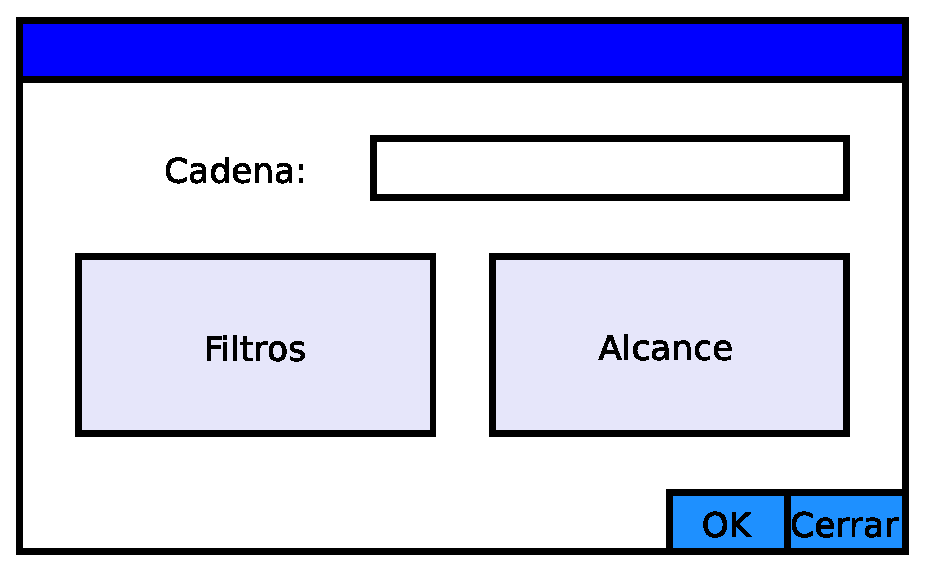
\includegraphics[height=.35\textheight]{desarrollo/prototiposInterfaz/dialogobusqueda}
  \caption{Prototipo del di�logo de b�squeda}
  \label{fig:proto_dlgbusqueda}
\end{figure}

\begin{figure}
  \centering
  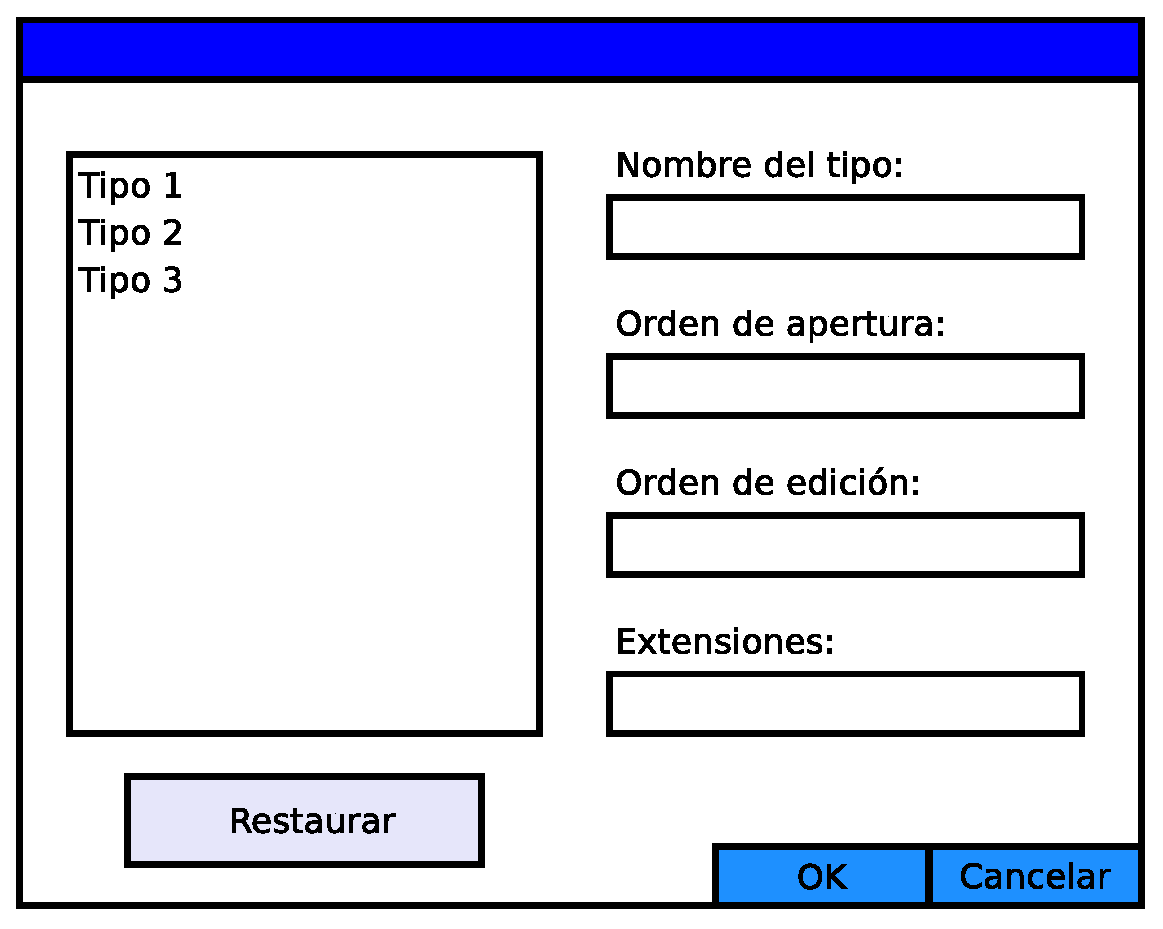
\includegraphics[width=.8\textwidth]{desarrollo/prototiposInterfaz/dialogotipos}
  \caption{Prototipo del di�logo de gesti�n de descriptores de formatos de documentos}
  \label{fig:proto_dlgdfd}
\end{figure}

\begin{figure}
  \centering
  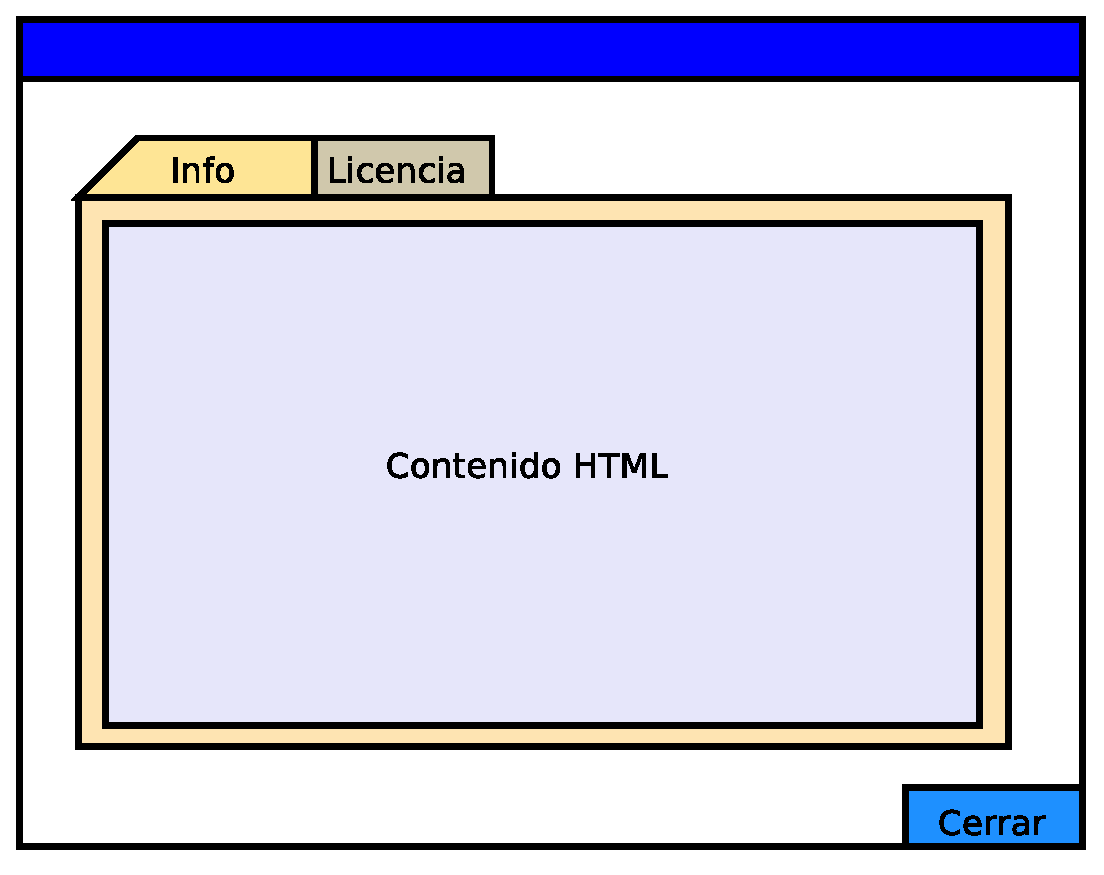
\includegraphics[height=.4\textheight]{desarrollo/prototiposInterfaz/dialogoacercade}
  \caption{Prototipo del di�logo de informaci�n del programa}
  \label{fig:proto_dlgacercade}
\end{figure}

\subsection{Funcionales}
\label{sec:req_func}

\index{requisitos!funcionales}

\begin{itemize}
\item Generar ficheros \ac{XML} que engloben la informaci�n de una
  fuente Lisp, su demostraci�n por \ac{ACL2} asociada y referencias a
  todas las otras fuentes Lisp (libros de \ac{ACL2}) de que dependa.

\item Permitir la visualizaci�n de documentos pertenecientes a
  lenguajes basados en \ac{YAML} 1.1, y la posterior creaci�n de hojas
  espec�ficas a �stos.

\item Navegar por m�ltiples documentos a la vez, abstrayendo al
  usuario si �ste lo desea de los detalles de la estructura de sus
  versiones \ac{XML}.

\item Mantener un historial de documentos recientes, f�cilmente
  accesible por el usuario.

\item Permitir editar los documentos visualizados con el editor
  favorito del usuario para el formato correspondiente, si est�n
  presentes en el sistema. Puede que en ciertos casos s�lo dispongamos
  del \ac{XML} final.

\item Regenerar cualquier documento abierto si se producen cambios en
  �l en alg�n momento, pudiendo mantener el editor y el visor abiertos
  a la vez.

\item Relacionar los elementos del documento entre s�, y con elementos
  espec�ficos de otros documentos.

\item Generar autom�ticamente informaci�n adicional que pueda ser de
  inter�s para el usuario.

\item Realizar b�squedas por el documento, sin p�rdidas de informaci�n
  respecto del texto original, usando diversos filtros y pudiendo
  limitar su alcance.

\item Repetir la �ltima b�squeda realizada.

\item Personalizar las �rdenes usadas para lanzar el editor o el
  conversor de cualquiera de los formatos aceptados, y volver a los
  ajustes por defecto en cualquier momento.

\item Cambiar el tipo y/o formato de la informaci�n mostrada durante
  la ejecuci�n del programa.
\end{itemize}

\subsection{Atributos del sistema software}
\label{sec:req_attr}

\index{requisitos!atributos}

En este proyecto, la mantenibilidad es fundamental para que
posteriores ampliaciones y correcciones se hagan de forma r�pida y
sencilla, dada la complejidad de la herramienta cuyo uso se pretende
facilitar.

Tambi�n ser�a deseable la separaci�n entre la l�gica de visualizaci�n
y el resto del sistema por la posibilidad de que los usuarios (v�ase
\S\ref{sec:desc_usuarios}) extiendan sus capacidades de visualizaci�n
sin tener que modificar el c�digo fuente del proyecto, s�lo
modificando o a�adiendo ficheros de datos. Separar la l�gica de
conversi�n de \visor{} de cuestiones espec�ficas a \postprocesador{}
posibilitar� su uso para formatos distintos a demostraciones de
\ac{ACL2}, y que tampoco tengan por qu� ser basados en \ac{XML}.

La transportabilidad, aunque no imprescindible, se corresponde con el
deseo de permitir un libre uso de este proyecto como una herramienta
m�s para los usuarios de \ac{ACL2} que limite en lo m�nimo posible su
elecci�n de sistema operativo.

Con vistas a ampliar la base de usuarios potencial de \visor{} y sus
extensiones, cobrar� importancia no solo la facilidad de uso, sino
tambi�n la facilidad de instalaci�n, controlando el n�mero de
dependencias externas y, cuando esto no sea posible, reduciendo su
impacto en la complejidad de la instalaci�n.

%%% Local Variables: 
%%% mode: latex
%%% TeX-master: "../memoria"
%%% End: 


\section{An�lisis del sistema}
\label{sec:analisis}
%%
%% analisis.tex
%% Copyright (C) 2008 Antonio Garc�a Dom�nguez
%% $Id: analisis.tex 612 2008-06-25 10:04:09Z antonio $
%%

\subsection{Historias de usuario}
\label{sec:historiasusuario}
%%
%% husuario.tex
%% Copyright (C) 2008 Antonio Garc�a Dom�nguez
%% $Id: husuario.tex 624 2008-07-02 21:40:46Z antonio $
%%

\index{historia de usuario|see{pr�ctica XP!historia de usuario}}

Como ya se coment� en \S\ref{sec:xp_practicas}
(p�gina~\pageref{sec:xp_practicas}), los proyectos basados en \ac{XP}
se estructuran en torno a las historias de los usuarios, que describen
un comportamiento o propiedad deseada del sistema en sus propias
palabras.

Mientras se redactan, el equipo de desarrolladores, tras realizar un
an�lisis superficial del trabajo implicado con ayuda del cliente,
asigna a cada historia un tiempo estimado de finalizaci�n en d�as
ideales y un riesgo. El cliente puede, en funci�n de esos factores y
de sus intereses, marcar la prioridad de una historia.

Una historia de usuario puede ser de muy alto nivel o de muy bajo
nivel, pudiendo unirse varias historias de bajo nivel en una sola, o
dividirse una de alto nivel en varias m�s sencillas.

Pasaremos a listar las historias de usuario que se han ido acumulando
a lo largo de la comunicaci�n con los clientes durante el desarrollo
del PFC, es decir, mis directores de proyecto, usuarios de \ac{ACL2} y
por lo tanto partes interesadas.

En los casos de \postprocesador{} y \yaxml{}, hay varias historias
pospuestas para futuras iteraciones, sin que ello impida entregar una
versi�n funcional (recordemos el principio ``Margen'' de \ac{XP}).

Dividiremos la mayor�a de las historias en tareas, dando estimaciones
iniciales del tiempo necesario para cada una. Otras ser�n lo bastante
concretas como para no necesitar ninguna subdivisi�n.

En esta lista de historias de usuario no se incluyen aquellas que se
completaron durante el Proyecto Fin de Carrera ``Post-procesador y
Visor de Demostraciones del Sistema ACL2''.

\subsubsection{\nombrevisor{}}
\label{sec:husuario_visor}

\begin{enumerate}
\item \label{item:multidoc}
  \begin{quote}
    ``A�adir soporte para visualizar varios ficheros a la vez y
    enlazarlos entre s�.''
  \end{quote}

  Esta historia de usuario es muy corta para todo el trabajo que
  implica:

  \begin{enumerate}
  \item Concentrar el estado de visualizaci�n del documento actual en
    un modelo de presentaci�n, para as� poder cambiar entre los
    estados de cada documento: 3 d�as ideales. Completada.

  \item Integrar de nuevo y depurar toda la funcionalidad de la
    aplicaci�n con este nuevo dise�o: 3 d�as ideales. Completada.

  \item A�adir una interfaz \ac{TDI} a XMLEye, y asegurar su
    integraci�n con el \emph{Look and Feel} instalado: 4 d�as
    ideales. Completada.

  \item A�adir la posibilidad de establecer hiperv�nculos entre varios
    documentos: 2 d�as ideales. Completada.
  \end{enumerate}

\item 
  \begin{quote}
    ``El visor no deber�a saber absolutamente nada de \ac{ACL2}. Nada
    en su interfaz gr�fica ni en su implementaci�n nos debe recordar
    que podemos trabajar con \ac{ACL2}. Pero s� podr�a saber algo de
    un procesador externo que tradujera ficheros de un formato, del
    que el visor tampoco sabe nada, a \ac{XML}. Tambi�n podr�a conocer
    la existencia de hojas de estilo \ac{XSLT} y de herramientas
    externas, como un editor, como de hecho ocurre ahora.''
  \end{quote}

  \begin{enumerate}
  \item Mover toda la l�gica propia de \ac{ACL2} a \postprocesador{},
    y retirarla de \visor{}: 0,5 d�a ideal para retirarla. V�ase la
    historia~\ref{item:integrar-pproc-acl2} de \postprocesador{} para
    la estimaci�n de su recreaci�n. Completada.

  \item Definir la estructura y contenidos de un descriptor de formato
    de documento: 0,5 d�a ideal. Completada.

  \item Implementar y depurar la estructura en 2 niveles del
    repositorio de descriptores, empleando ciertas variables del
    entorno si se hallan definidas: 2 d�as ideales. Completada.

  \item Internacionalizar las cadenas contenidas en los descriptores:
    0,5 d�a ideal. Completada.

  \item Integrar la informaci�n de los descriptores con los controles
    de apertura y edici�n de documentos: 2 d�as ideales. Completada.

  \item Crear un di�logo de gesti�n de los descriptores instalados: 1
    d�a ideal. Completada.
  \end{enumerate}

\item 
  \begin{quote}
    ``Vigilar directamente el fichero fuente en caso de cambios, en vez de
    solamente cuando se cierra el editor. As�, si uno abre el editor, hace
    un par de cambios y guarda (sin cerrar el editor), tambi�n se
    actualizar�. En caso de que se desactive temporalmente la
    reimportaci�n autom�tica, tambi�n deber�a funcionar correctamente si
    en ese intervalo se hicieron cambios.''
  \end{quote}

  Esta historia implica:

  \begin{itemize}
  \item Resolver unas condiciones de carrera conocidas que produc�an
    fallos intermitentes en la reimportaci�n autom�tica. Tiempo
    estimado: 1 d�a ideal. Completada.

  \item Refinar el dise�o del momento para evitar que al reabrir el
    documento, apareciera como una nueva pesta�a. Tiempo estimado: 1
    d�a ideal. Completada.

  \item Implementar la detecci�n y notificaci�n con un hilo pausable
    de baja prioridad en segundo plano, activado de forma
    intermitente. Tiempo estimado: 1 d�a ideal. Completada.
  \end{itemize}

\end{enumerate}

\subsubsection{\nombrepostprocesador{}}
\label{sec:husuario_pproc}

\begin{enumerate}
\item 
  \begin{quote}
    ``Normalizar la estructura de \postprocesador{} para que siga la de
    un m�dulo del CPAN y se porte mejor a la hora de en el futuro
    hacer un paquete Debian.''
  \end{quote}

  Tiempo estimado: 2 d�as ideales. Completada.

\item 
  \begin{quote}
    ``Llevar la cuenta de en qu� paquete (espacio de nombres) estamos
    trabajando. Puede saberse por el indicador (prompt).''
  \end{quote}

  Se requerir�a a�adir el filtrado de la orden \orden{in-package} y
  del indicador de \ac{ACL2}, modificando en consecuencia la salida
  \ac{XML}.

  Tiempo estimado: 1 d�a ideal. Completada.

\item \label{item:hanoi}

  \begin{quote}
    ``Tratar el ejemplo de las Torres de Hanoi de~\cite{Hanoi},
    dividi�ndolo en tres partes: \fichero{books/hanoi.lisp}, libro que
    define el algoritmo para resolver el problema y todo lo necesario
    excepto el propio teorema del n�mero de intercambios;
    \fichero{books/hanoi.acl2}, que se encarga de definir el paquete y
    certificar el libro; y \fichero{hanoi-use.lisp}, que incluye el
    libro y contiene el teorema con el n�mero de intercambios.''
  \end{quote}

  Una vez la capacidad de visualizar y enlazar entre s� varios
  documentos est� a�adida en \visor{} (v�ase su
  historia~\ref{item:multidoc}), habr�a que:

  \begin{itemize}
  \item Crear un m�dulo de detecci�n de dependencias que utilice un
    simple an�lisis superficial de sus �rdenes, de forma recursiva, y
    genere un �ndice de cada libro con los identificadores de los
    eventos que define y los libros de que depende a su vez. Tiempo
    estimado: 3 d�as ideales. Completada.

  \item Implementar el procesamiento de la salida de los eventos
    \orden{include-book}, \orden{certify-book}, \orden{defpkg} e
    \orden{in-package}. Tiempo estimado: 2 d�as ideales. Completada.
  \end{itemize}

\item 

  \begin{quote}
    ``Mejorar los informes de errores de las pruebas de regresi�n,
    evitando que fallen con diferencias insignificantes.''
  \end{quote}

  Requiere:

  \begin{itemize}
  \item Volver a implementar las pruebas de regresi�n, esta vez
    calculando la diferencia entre los documentos no a partir de las
    l�neas de texto que lo componen, sino usando el �rbol DOM
    resultado de analizar los dos documentos \ac{XML}. Tiempo
    estimado: 2 d�as ideales. Completado.

  \item Implementar el c�digo necesario para ignorar aquellas
    diferencias que no sean de inter�s. Tiempo estimado: 1 d�a
    ideal. Completado.
  \end{itemize}

\item \label{item:integrar-pproc-acl2}

  \begin{quote}
    ``Integrar \postprocesador{} con ACL2, haciendo que
    autom�ticamente genere las salidas y las sit�e en ficheros
    \fichero{.out} y \fichero{.xml} en el mismo directorio, realizando
    una gesti�n de dependencias al estilo GNU Make entre ellos y la
    fuente Lisp. As� evitar�amos importar varias veces el mismo
    fichero, y se podr�a simplificar el visor.''
  \end{quote}

  Una vez est� terminada la tarea~\ref{item:hanoi}, habr�a que
  modificar el c�digo que recibe el texto de la demostraci�n de
  \ac{ACL2} y lanza el proceso de an�lisis para que invoque �l mismo a
  \ac{ACL2} en caso de que el fichero \fichero{.xml} no exista o se
  halle desactualizado respecto a la fuente Lisp.

  Tiempo estimado: 1 d�a ideal. Completada.

\item 

  \begin{quote}
    ``Manejar los eventos definidos por el usuario con
    \orden{make-event} y las expansiones de macros creadas con
    \orden{defmacro}.''
  \end{quote}

  No est� del todo clara la forma de resolver esta historia de
  usuario. Un an�lisis superficial sugiere esta divisi�n en tareas:

  \begin{itemize}
  \item Instrumentar el c�digo Lisp con llamadas previas a
    \verb#:trans1# sobre la orden desconocida, sin que se produzcan
    modificaciones en el espaciado de cualquiera del resto de las
    l�neas del documento. Tiempo estimado: 2 d�as ideales. Pospuesta.

  \item Usar la orden resultante de \verb#:trans1# como el enunciado
    de la orden para la siguiente salida. Tiempo estimado: 2 d�as
    ideales, por posibles cambios importantes a realizar en el
    dise�o. Pospuesta.

  \item Registrar de alguna forma la expansi�n producida por
    \orden{make-event}, tomando como base el fichero fuente
    \fichero{basic.lisp} del libro \fichero{make-event} incluido en la
    distribuci�n de \ac{ACL2}. Tiempo estimado: 3 d�as
    ideales. Pospuesta.
  \end{itemize}

\item 

  \begin{quote}
    ``Tratar el caso en que un \orden{include-book} aparezca dentro de un
    \orden{local} (y entonces lo que se incluye es local al libro, no se ve
    fuera). Y esto puede aparecer dentro de un \orden{encapsulate}''.
  \end{quote}

  Hay que refinar la sintaxis de los grafos de dependencias para
  incluir menciones al �mbito de validez de cada entrada: puede que
  dentro de un \orden{encapsulate} se haga referencia a un evento
  \evento{P::F}, y en el nivel global u otro \orden{local} o
  \orden{encapsulate}, se dependa de otro evento distinto con el mismo
  nombre. Limitando el alcance de las definiciones se podr�a tratar
  este problema.

  Tiempo estimado: 3 d�as ideales. Pospuesta.

\item 

  \begin{quote}
    ``Tratar las \emph{forcing rounds}, demostraciones realizadas tras
    la demostraci�n principal sobre cualquier hip�tesis cuya
    aplicaci�n se hubiera forzado durante la demostraci�n anterior (la
    demostraci�n inicial, u otra \emph{forcing round}).''
  \end{quote}
  
  Hay que refinar la divisi�n jer�rquica de las metas y procesar la
  salida espec�fica a las \emph{forcing rounds} estableciendo los
  enlaces correspondientes.

  Tiempo estimado: 3 d�as ideales. Pospuesta.

\item
  \begin{quote}
    ``Tratar todas las opciones que pueden acompa�ar a un \orden{defthm} y a
    un \orden{defun}.''
  \end{quote}

  En el caso de \orden{defthm}, se han de tratar \orden{:rule-classes},
  \orden{:instructions}, \orden{:hints}, \orden{:otf-flg} y
  \orden{:doc}.

  Para \orden{defun}, se han de tratar las declaraciones y la cadena
  de documentaci�n (del estilo del argumento de \orden{:doc}).

  Esta historia se habr�a de dividir entonces en varias tareas
  independientes:
  \begin{enumerate}
  \item Soporte para cadenas de documentaci�n, \orden{:rule-classes} y
    \orden{:otf-flg}: 2 d�as ideales. Completada parcialmente.
  \item Soporte de \orden{:instructions}: 2 d�as ideales. Pospuesta.
  \item Soporte de \orden{:hints}: 2 d�as ideales. Pospuesta.
  \item Soporte de declaraciones (incluye \orden{:hints} e
    \orden{:instructions}): 2 d�as ideales. Pospuesta.
  \end{enumerate}

\item
  \begin{quote}
    ``Marcar las salidas de los nuevos apuntes de
    Moore~\cite{recindacl2}, \emph{Recursion and Induction}.''
  \end{quote}

  El trabajo necesario para implementar esta historia de usuario es
  extensivo, requiriendo implementar todas las historias anteriormente
  propuestas, y a�adir la capacidad a \postprocesador{} de tratar
  macros Lisp.  

  Tiempo estimado: 6 d�as ideales. Pospuesta.

\end{enumerate}

\subsubsection{\nombreyaxml{}}
\label{sec:husuario_yaxml}

\begin{enumerate}
\item 
  \begin{quote}
    ``Abrir documentos \ac{YAML} en \nombrevisor{} sin que suponga una
    p�rdida o alteraci�n de la informaci�n disponible.''
  \end{quote}

  \begin{itemize}
  \item Seleccionar un m�dulo Perl que permita cargar documentos
    \ac{YAML}. Idealmente, deber�a ser Perl puro, pero la velocidad de
    carga y la fiabilidad son m�s importantes. Tiempo estimado: 0,5 d�a
    ideal. Completada.

  \item Definir un primer prototipo del m�dulo que verifique la
    viabilidad del enfoque usado con algunos ejemplos sencillos: 0,5
    d�a ideal. Completada.

  \item Convertir el prototipo en un m�dulo completo al estilo del
    \ac{CPAN}, con pruebas de unidad basadas en Perl que verifiquen la
    conservaci�n de la informaci�n: 1 d�a ideal. Completada.
  \end{itemize}

\item 
  \begin{quote}
    ``Procesar el ejemplo de la factura de la web~\cite{YAXML} de \ac{YAXML}.''
  \end{quote}

  Hay que establecer un mecanismo para detectar la existencia de
  anclas y alias en la estructura de datos generada en memoria,
  evitando tener que volver a analizar el c�digo fuente
  \ac{YAML}. Podr�an buscarse referencias duplicadas, por
  ejemplo. Tiempo estimado: 1 d�a ideal. Completada.

\item 
  \begin{quote}
    ``Preparar hojas de estilos para los marcadores de Firefox y
    volcados del entorno de desarrollo web Django.''
  \end{quote}

  \begin{itemize}
  \item Comprobar que la biblioteca usada analiza correctamente
    documentos del subconjunto \ac{JSON} de \ac{YAML} 1.1 que emplean
    los volcados de Django y los marcadores de Firefox, y en caso
    contrario reemplazar la existente. Tiempo estimado: 1 d�a ideal. Completada.

  \item Comprobar que se procesan debidamente documentos codificados
    en \acs{UTF}-8 con caracteres fuera del conjunto \acs{ASCII} de 7
    bits. Tiempo estimado: 1 d�a ideal. Completada.

  \item Implementar hojas de estilos especializadas para los
    marcadores de Firefox y volcados de Django. Tiempo estimado: 2
    d�as ideales. Pospuesta.
  \end{itemize}

\end{enumerate}

%%% Local Variables: 
%%% mode: latex
%%% TeX-master: "../../memoria"
%%% End: 


\subsection{Casos de uso}
\label{sec:casosuso}
%%
%% Casos de uso de XMLEye
%% Copyright (C) 2008 Antonio Garc�a Dom�nguez
%% $Id: casosuso.tex 629 2008-07-06 13:47:58Z antonio $
%%
\index{meta de usuario|see{casos de uso!meta de usuario}}
\index{subfunci�n|see{casos de uso!subfunci�n}}
\index{casos de uso!meta de usuario}
\index{casos de uso!subfunci�n}

Estos casos de uso nos permiten analizar de manera general y abstracta
qu� es lo que se requiere en conjunto de las historias de usuario de
\visor{} de este Proyecto y la versi�n del Proyecto Fin de Carrera
sobre el que se basa. El diagrama que ilustra las relaciones entre los
distintos casos de uso que cumplen las metas del usuario se puede
hallar en la figura~\ref{fig:diag_casosdeuso}.

El l�mite del sistema establecido engloba �nicamente a \visor{}. Los
conversores externos, entre los cuales se hallan \postprocesador{} y
\visor{}, participan �nicamente como un agente externo. El m�todo de
comunicaci�n con \visor{} se aclarar� m�s tarde, en la fase de
dise�o. A menos que se indique lo contrario, los casos de uso aqu�
mostrados son en general de nivel de meta de usuario.

\begin{figure}
  \centering
  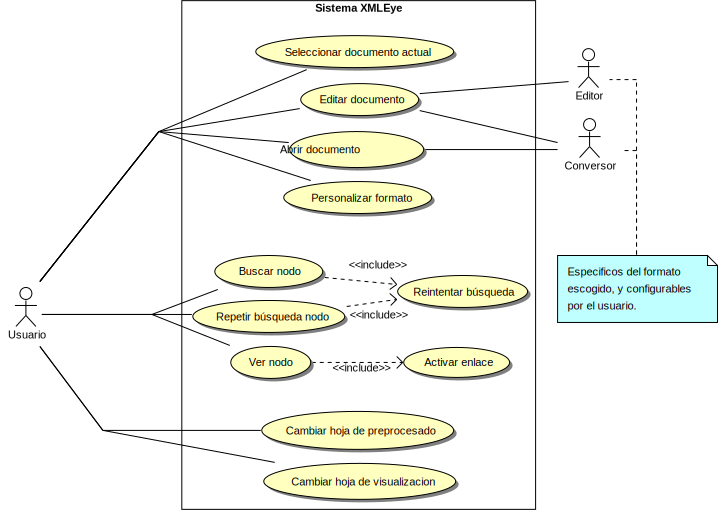
\includegraphics[width=\textwidth]{desarrollo/analisis/casosuso}
  \caption{Diagrama de casos de uso}
  \label{fig:diag_casosdeuso}
\end{figure}

\subsubsection{Seleccionar documento actual}
\label{sec:seleccionar_doc_actual}

\begin{description}
\item[Actor principal] Usuario: desea seleccionar el documento sobre
  el que actuar en el resto de casos de prueba de entre los documentos
  abiertos.
\item[Precondiciones] Existe al menos un documento abierto.
\item[Postcondiciones] Se muestra el documento seleccionado.

\item[Escenario principal] \mbox{}
  \begin{enumerate}
  \item El usuario indica su intenci�n de cambiar de documento.
  \item El sistema proporciona una lista de los documentos disponibles.
  \item El usuario selecciona el documento de la lista. \label{item:select_doc}
  \item El sistema registra la selecci�n, guarda el estado actual de
    la visualizaci�n actual y restaura el estado de la visualizaci�n
    del documento seleccionado, mostr�ndolo tal y como estaba antes de
    haber seleccionado otro documento.
  \end{enumerate}

\item[Variaciones] \mbox{}

  \begin{enumerate}[{\ref{item:select_doc}}a.]
  \item El documento es el mismo que el actual:
    \begin{enumerate}[1.]
    \item El sistema cancela el cambio de uso.      
    \end{enumerate}
  \end{enumerate}

\end{description}

\subsubsection{Editar documento}
\label{sec:casouso_editar}

\begin{description}
\item[Actor principal] Usuario: desea editar en paralelo a la
  visualizaci�n el enunciado fuente del documento actual de forma r�pida
  y sencilla usando su editor preferido.
\item[Actores secundarios] \mbox{}
  \begin{description}
  \item[Editor] Editor preferido del usuario para el formato del
    documento actual.
  \item[Conversor] Sistema externo ocupado de convertir el documento a
    \ac{XML}, si es necesario.
  \end{description}
\item[Precondiciones] Existe un documento abierto.
\item[Postcondiciones] Se ha abierto el documento con el editor
  especificado en el descriptor de formato correspondiente.
\item[Escenario principal] \mbox{}
  \begin{enumerate}
  \item El usuario indica su intenci�n de editar el enunciado del
    documento abierto.
  \item El sistema lanza el editor, y contin�a con su funcionamiento
    normal, esperando en segundo plano a que se realicen cambios.
    \label{item:edit_espera}
  \item El usuario guarda algunos cambios en el documento.
  \item El sistema detecta los cambios: se regenera la visualizaci�n
    completa del documento.
  \item El sistema pasa de nuevo a la espera de m�s cambios en segundo
    plano.
  \end{enumerate}

\item[Variaciones] \mbox{}

  \begin{enumerate}[{\ref{item:edit_espera}}a.]
  \item La invocaci�n del editor ha fallado:
    \begin{enumerate}[1.]
    \item El sistema indica el error y cancela el caso de uso.
    \end{enumerate}

  \item Se ha cerrado el documento:
    \begin{enumerate}[1.]
    \item El sistema deja de monitorizar el documento.
    \end{enumerate}
  \end{enumerate}

\end{description}

\subsubsection{Abrir documento}
\label{sec:casouso_abrir}

\begin{description}
\item[Actor principal] Usuario: desea examinar la versi�n m�s reciente
  del documento en general, para despu�s centrarse en los nodos de su
  inter�s.
\item[Actores secundarios] Conversor: sistema externo que se ocupa de
  convertir el documento proporcionado a \ac{XML}.
\item[Precondiciones] Ninguna.
\item[Postcondiciones] Se carga la versi�n m�s reciente del documento
  elegido por el usuario.
\item[Escenario principal]\mbox{}
  \begin{enumerate}
  \item El usuario indica su intenci�n de abrir un documento ya
    existente.
  \item El sistema muestra los documentos disponibles.
  \item El usuario selecciona un
    documento. \label{item:abrir_cancelar}
  \item El sistema comprueba que el documento
    existe. \label{item:abrir_docexiste}
  \item El sistema le asocia el primer formato con una extensi�n
    coincidente, y aplica su conversor, si tiene uno asociado, al
    documento. \label{item:abrir_asociar_formato}.
  \item El sistema muestra el documento elegido, tras a�adirlo a la
    lista de documentos abiertos.
  \end{enumerate}
\item[Variaciones]\mbox{}

  \begin{enumerate}[{\ref{item:abrir_cancelar}}a.]
  \item El usuario cancela la selecci�n de documento:
    \begin{enumerate}[1.]
    \item El sistema cancela el caso de uso.
    \end{enumerate}
  \end{enumerate}

  \begin{enumerate}[{\ref{item:abrir_docexiste}}a.]
  \item El documento no existe:
    \begin{enumerate}[1.]
    \item El sistema muestra el error y cancela el caso de uso.
    \end{enumerate}
  \end{enumerate}

  \begin{enumerate}[{\ref{item:abrir_asociar_formato}}a.]
  \item No existe un formato con una extensi�n coincidente:
    \begin{enumerate}[1.]
    \item El sistema utiliza el formato por defecto, \ac{XML}, que no
      tiene un conversor asociado.
    \end{enumerate}
  \end{enumerate}
\end{description}

\subsubsection{Personalizar formato}
\label{sec:personalizar_formato}

\begin{description}
\item[Actor principal] Usuario: desea cambiar las opciones de alguno
  de los formatos instalados.

\item[Precondiciones] Existe al menos un formato instalado en el
  sistema.

\item[Postcondiciones] Se cambian los ajustes locales del usuario para
  el formato indicado, sin cambiar los ajustes globales.

\item[Escenario principal] \mbox{}
  \begin{enumerate}
  \item El usuario indica su intenci�n de cambiar las opciones de alguno de
    los formatos.

  \item El sistema muestra la lista de los formatos disponibles. \label{item:pers_primero}

  \item El usuario selecciona un formato de la lista.

  \item El sistema muestra los campos modificables del formato:

    \begin{itemize}
    \item La traducci�n del nombre del formato que se ajuste mejor a
      la localizaci�n activa por defecto en el entorno del usuario.
    \item La orden usada para invocar al editor preferido del usuario
      para dicho formato.
    \item La orden usada para invocar al conversor a \ac{XML}
      preferido del usuario para dicho formato.
    \item La lista de extensiones, separadas por comas, con las que se
      asociar� a este formato.
    \end{itemize}
    
  \item El usuario modifica el valor de los campos. 

  \item El sistema solicita confirmaci�n al usuario.

  \item El usuario proporciona la confirmaci�n. \label{item:pers_conf}

  \item El sistema registra los cambios a nivel del usuario actual,
    sin modificar los ajustes globales, y los hace efectivos a partir
    del mismo momento.
  \end{enumerate}

\item[Variaciones] \mbox{}

  \begin{enumerate}[{\ref{item:pers_primero}-\ref{item:pers_conf}}a.]
  \item El usuario cancela la personalizaci�n:
    \begin{enumerate}[1.]
    \item El sistema cancela el caso de uso, sin que se hagan
      efectivos los campos.
    \end{enumerate}
  \end{enumerate}

  \begin{enumerate}[{\ref{item:pers_conf}}a.]
  \item Los campos de nombre del formato, orden de edici�n o
    extensiones se hallan vac�os o s�lo contienen espacios en blanco,
    alguna de las extensiones pasadas contiene espacios o est� vac�a,
    o la orden de importaci�n contiene solamente uno o m�s espacios en
    blanco:
    \begin{enumerate}[1.]
    \item El sistema informa de la situaci�n y solicita corregir dicha
      situaci�n.
    \end{enumerate}
  \end{enumerate}

\end{description}

\subsubsection{Buscar nodo}
\label{sec:casouso_buscarnodo}

\begin{description}
\item[Actor principal] Usuario: desea localizar r�pidamente los nodos
  que cumplan una serie de condiciones.
\item[Precondiciones] Hay un documento abierto.
\item[Postcondiciones] Se muestra el resultado de la b�squeda.
\item[Escenario principal] \mbox{}
  \begin{enumerate}
  \item El usuario indica su intenci�n de iniciar una nueva b�squeda.
    \label{item:buscar_inicio}
  \item El sistema solicita la clave de b�squeda.
  \item El usuario introduce la clave de b�squeda.
  \item El sistema comprueba que la clave de b�squeda es v�lida.
    \label{item:buscar_chkclave}
  \item El sistema presenta al usuario las opciones de filtrado.
  \item El usuario elige las opciones de filtrado.
    \label{item:buscar_filtro}
  \item El sistema realiza la b�squeda a partir del nodo actual y
    muestra el primer resultado. \label{item:buscar_res}
  \end{enumerate}
\item[Variaciones] \mbox{}
  
  \begin{enumerate}[{\ref{item:buscar_inicio}-\ref{item:buscar_filtro}}a.]
  \item El usuario cancela la b�squeda:
    \begin{enumerate}[1.]
    \item El sistema cancela el caso de uso.
    \end{enumerate}
  \end{enumerate}
  
  \begin{enumerate}[{\ref{item:buscar_chkclave}}a.]
  \item La clave no es v�lida:
    \begin{enumerate}[1.]
    \item El sistema indica el error y pide una nueva clave.
    \end{enumerate}
  \end{enumerate}
  
  \begin{enumerate}[{\ref{item:buscar_res}}a.]
  \item No hay resultados:
    \begin{enumerate}[1.]
    \item \emph{include(Reintentar b�squeda)}
    \end{enumerate}
  \end{enumerate}
\end{description}

\subsubsection{Repetir b�squeda}
\label{sec:casouso_repbusqueda}

\begin{description}
\item[Actor principal] Usuario: desea encontrar otro nodo que cumpla
  las mismas condiciones que el anterior, sin tener que volver a
  especificar las opciones de filtrado.
\item[Precondiciones] Hay un documento abierto.
\item[Postcondiciones] Se muestra el siguiente nodo que cumple las
  condiciones de la �ltima b�squeda.
\item[Escenario principal] \mbox{}

  \begin{enumerate}
  \item El usuario desea repetir la b�squeda anterior:
  \item El sistema comprueba que existe una b�squeda anterior.
    \label{item:chk_busqanterior}
  \item El sistema realiza de nuevo la b�squeda a partir del nodo
    actual y muestra el primer resultado.
    \label{item:repetirbusq_buscar_res}
  \end{enumerate}

\item[Variaciones] \mbox{}

  \begin{enumerate}[{\ref{item:chk_busqanterior}}a.]
  \item No existen b�squedas anteriores:
    \begin{enumerate}[1.]
    \item El sistema indica el error y cancela el caso de uso.
    \end{enumerate}
  \end{enumerate}
  
  \begin{enumerate}[{\ref{item:repetirbusq_buscar_res}}a.]
  \item No hay resultados:
    \begin{enumerate}[1.]
    \item \emph{include(Reintentar b�squeda)}
    \end{enumerate}
  \end{enumerate}
\end{description}

\subsubsection{Reintentar b�squeda}
\label{sec:casouso_reintentar_busq}

\begin{description}
\item[Actor principal] Usuario: desea visualizar un nodo que cumpla
  las condiciones, aunque tenga que relajar el alcance de la b�squeda.
\item[Nivel de caso de uso] Subfunci�n.
\item[Precondiciones] Hay un documento abierto.
\item[Postcondiciones] Se muestra el primer nodo que cumple las nuevas
  condiciones relajadas.
\item[Escenario principal] \mbox{}
  \begin{enumerate}
  \item El sistema indica la situaci�n y ofrece repetir la b�squeda
    con par�metros m�s generales.
  \item El usuario acepta. \label{item:buscar_res_aceptar}
  \item El sistema relanza la b�squeda y muestra el primer
    resultado. \label{item:buscar_res_repetir}
  \end{enumerate}

\item[Variaciones] \mbox{}
  \begin{enumerate}[{\ref{item:buscar_res_aceptar}}a.]
  \item El usuario rechaza la oferta: 
    \begin{enumerate}[1.]
    \item El sistema cancela el caso de uso.
    \end{enumerate}
  \end{enumerate}

  \begin{enumerate}[{\ref{item:buscar_res_repetir}}a.]
  \item No hay resultados:
    \begin{enumerate}[1.]
    \item El sistema indica la situaci�n y cancela el caso de uso.
    \end{enumerate}
  \end{enumerate}
\end{description}

\subsubsection{Ver nodo}
\label{sec:casouso_selnodo}

\begin{description}
\item[Actor principal] Usuario: desea visualizar la informaci�n acerca
  de un nodo del documento.
\item[Precondiciones] Hay un documento abierto.
\item[Postcondiciones] Se muestra la informaci�n del nodo seleccionado.
\item[Escenario principal] \mbox{}
  \begin{enumerate}
  \item El usuario indica el nodo del documento que desea ver.
  \item El sistema comprueba que existe. \label{item:selnode_chknode}
  \item El sistema muestra la informaci�n del nodo al usuario, dejando
    que interact�e con �l. \label{item:selnode_interact}
  \end{enumerate}
\item[Variaciones] \mbox{}

  \begin{enumerate}[{\ref{item:selnode_chknode}}a.]
  \item El nodo no existe:
    \begin{enumerate}[1.]
    \item El sistema muestra una visualizaci�n vac�a.
    \end{enumerate}
  \end{enumerate}

  \begin{enumerate}[{\ref{item:selnode_interact}}a.]
  \item El usuario activa uno de los hiperv�nculos disponibles:
    \begin{enumerate}[1.]
    \item \emph{include(Activar enlace)}
    \end{enumerate}
  \end{enumerate}

\end{description}

\subsubsection{Activar enlace}
\label{sec:casouso_activar_enlace}

\begin{description}
\item[Actor principal] Usuario: desea visualizar el recurso al que
  se�ala el enlace activado.
\item[Nivel de caso de uso] Subfunci�n.
\item[Precondiciones] Hay un documento abierto, y se est� visualizando
  un nodo.
\item[Postcondiciones] Se muestra el destino del enlace pulsado, si
  tiene uno definido.
\item[Escenario principal] \mbox{}
  \begin{enumerate}
  \item El usuario activa el enlace en cuesti�n de la visualizaci�n
    del nodo actual.

  \item Si el enlace se�ala a otro nodo, se ejecuta el caso de uso
    ``Ver nodo'' sobre �l, y se termina el caso de uso.

  \item Si el enlace se�ala a una \ac{URL}, se muestra el documento en
    uno de los navegadores Web disponibles, y se termina el caso de uso.

  \item Si el enlace se�ala a un ancla de la visualizaci�n \ac{HTML}
    del nodo actual, se desplaza la posici�n actual a la del ancla, y
    se termina el caso de uso.

  \item Si el enlace se�ala a un nodo de otro documento, se visualiza
    dicho documento mediante ``Visualizar documento'', posteriormente
    se ejecuta ``Ver nodo'' sobre el nodo especificado, y se termina
    el caso de uso.

  \item El sistema cancela el caso de uso.
  \end{enumerate}

\end{description}

\subsubsection{Cambiar hoja de preprocesado}
\label{sec:casouso_hoja_preproc}

\begin{description}
\item[Actor principal] Usuario: desea cambiar la forma en
  que se muestra la estructura del documento.

\item[Precondiciones] Existe al menos un documento abierto y
  seleccionado.

\item[Postcondiciones] Se le muestra al usuario la nueva estructura
  del documento, procesada desde el texto \ac{XML} original a trav�s
  de la hoja seleccionada. Se usar� esta hoja para todos los ficheros
  que se abran a continuaci�n.

\item[Escenario principal] \mbox{}
  \begin{enumerate}
  \item El usuario indica su intenci�n de cambiar la hoja
    de preprocesado en uso. \label{item:cambio_hoja_inicio}
  \item El sistema muestra una lista de las hojas de preprocesado
    disponibles.
  \item El usuario selecciona una hoja de la
    lista. \label{item:cambio_hoja_selecc}
  \item El sistema recupera el texto \ac{XML} original del documento y
    lo procesa mediante la nueva hoja seleccionada.
  \item El sistema muestra la nueva estructura del documento, y vac�a
    la visualizaci�n del nodo actual, al no haber ninguno
    seleccionado.
  \item El sistema registra la hoja seleccionada como hoja de
    preprocesado por defecto para todos los documentos abiertos en
    adelante.
  \end{enumerate}

\item[Variaciones] \mbox{}

  \begin{enumerate}[{\ref{item:cambio_hoja_inicio}-\ref{item:cambio_hoja_selecc}}a.]
  \item El usuario cancela la selecci�n:
    \begin{enumerate}[1.]
    \item El sistema cancela la ejecuci�n del caso de uso.
    \end{enumerate}
  \end{enumerate}

\end{description}

\subsubsection{Cambiar hoja de visualizaci�n}
\label{sec:casouso_hoja_visualizacion}

\begin{description}
\item[Actor principal] Usuario: desea cambiar la forma en que se
  muestra la informaci�n de los nodos de un documento.

\item[Precondiciones] Existe al menos un documento abierto y
  seleccionado.

\item[Postcondiciones] Se visualiza el nodo actual y todos los
  posteriormente seleccionados en el documento actual y en todos los
  documentos abiertos posteriormente bajo la nueva hoja.

\item[Escenario principal] \mbox{}
  \begin{enumerate}
  \item El usuario indica su intenci�n de cambiar la hoja de
    visualizaci�n para el documento actual. \label{item:cambio_hoja_v_inicio}
  \item El sistema muestra la lista de las hojas de visualizaci�n
    disponibles.
  \item El usuario selecciona una de las hojas de la
    lista. \label{item:cambio_hoja_v_selecc}
  \item El sistema actualiza la visualizaci�n del nodo actualmente
    seleccionado, si lo hay.
  \item El sistema registra la hoja seleccionada como hoja de
    visualizaci�n por defecto para los documentos abiertos de ahora en
    adelante.
  \end{enumerate}
\item[Variaciones] \mbox{}

  \begin{enumerate}[{\ref{item:cambio_hoja_v_inicio}-\ref{item:cambio_hoja_v_selecc}}a.]
  \item El usuario cancela la selecci�n:
    \begin{enumerate}[1.]
    \item El sistema cancela la ejecuci�n del caso de uso.
    \end{enumerate}
  \end{enumerate}

\end{description}

%%% Local Variables: 
%%% mode: latex
%%% TeX-master: "../../memoria"
%%% End: 


\subsection{Modelo conceptual de datos del dominio de \acs{ACL2}}
\label{sec:datos_conceptual_acl2}
%%
%% datosconceptual.tex
%% $Id: datosconceptual_acl2.tex 617 2008-06-28 17:00:10Z antonio $ 
%%

\subsubsection{Notaci�n}
\label{sec:conceptual_notacion}

Se ha usado \ac{UML} 2.0, con las siguientes modificaciones:
\begin{itemize}
\item Por claridad, algunas clases se hallan duplicadas en los
  diagramas. Para evitar confusiones, las duplicaciones ocultan los
  atributos y se hallan en color azul.
\item Igualmente, se han omitido las multiplicidades unitarias en las
  asociaciones y composiciones.
\end{itemize}

\subsubsection{Descripci�n general}
\label{sec:conceptual_acl2_general}

Para \postprocesador{}, los conceptos a tratar son entes abstractos
relacionados con el proceso de demostraci�n de \ac{ACL2}.

As�, partimos de un \clase{Enunciado}, colecci�n de \clase{Orden}es de
\ac{ACL2} que produce una \clase{Demostraci�n}. Esta
\clase{Demostraci�n} asocia a cada \clase{Orden} un \clase{Resultado}
con la salida obtenida de \ac{ACL2}. Esta contendr� diversos tipos de
informaci�n seg�n la \clase{Orden} usada.

Puede que nuestro \clase{Enunciado} sea la ra�z de un proyecto de
\ac{ACL2}, y se halle definido en base a una serie de definiciones ya
demostradas en \clase{Libro}s existentes. Es importante ver que un
\clase{Libro} puede requerir de una serie de definiciones previas a su
vez: seg�n la terminolog�a de \ac{ACL2}, ser�a su \emph{mundo
  inicial}. Todo \clase{Evento} pertenece a un \clase{Paquete}: si no
se indica su nombre previamente con una orden \orden{in-package}, ser�
``ACL2''.

Adicionalmente, pueden aparecer avisos, errores y observaciones de
\ac{ACL2} al inicio del resultado de la ejecuci�n de una \clase{Orden}
dada.

A su vez, cada \clase{Resultado}, en caso de necesitar demostrar
alguna S-expresi�n, usar� una \clase{Meta} principal, que se podr�
dividir recursivamente en submetas. Cada \clase{Meta} usa un
determinado \clase{Proceso} de demostraci�n.

Se ha dividido el diagrama de clases conceptuales en tres:
\begin{enumerate}
\item Visi�n general del dominio del problema:
  figura~\ref{fig:conceptual_general} de la
  p�gina~\pageref{fig:conceptual_general}.

\item Tipos de Orden: figura~\ref{fig:conceptual_ordenes} de la
  p�gina~\pageref{fig:conceptual_ordenes}.

  Es interesante ver c�mo algunas �rdenes utilizan a otras. Por
  ejemplo, como paso de verificaci�n tras la certificaci�n de un libro
  con \orden{certify-book}, se intentan cargar sus contenidos en el
  mundo de \ac{ACL2}, justo como si se hubiera ejecutado una orden
  \orden{include-book}.

\item Tipos de Proceso: figura~\ref{fig:conceptual_procesos} de la
  p�gina~\pageref{fig:conceptual_procesos}.

\end{enumerate}

\begin{sidewaysfigure}
  \centering
  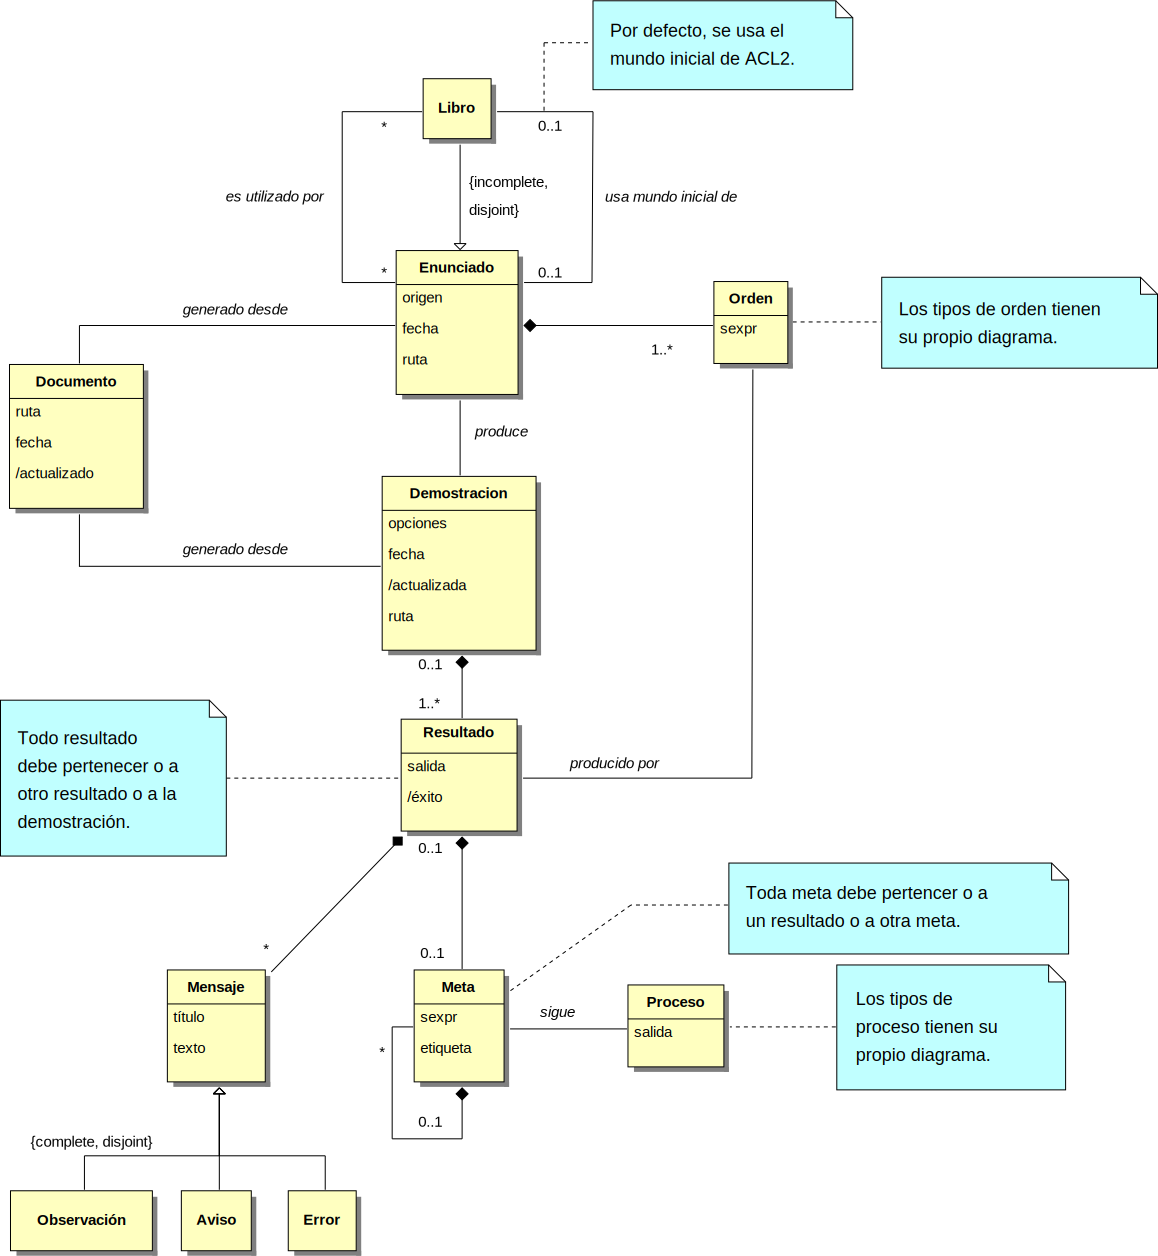
\includegraphics[height=.7\textheight]{desarrollo/analisis/modacl2_general}
  \caption{Diagrama de clases conceptuales general de \acs{ACL2}}
  \label{fig:conceptual_general}
\end{sidewaysfigure}

\begin{sidewaysfigure}
  \centering
  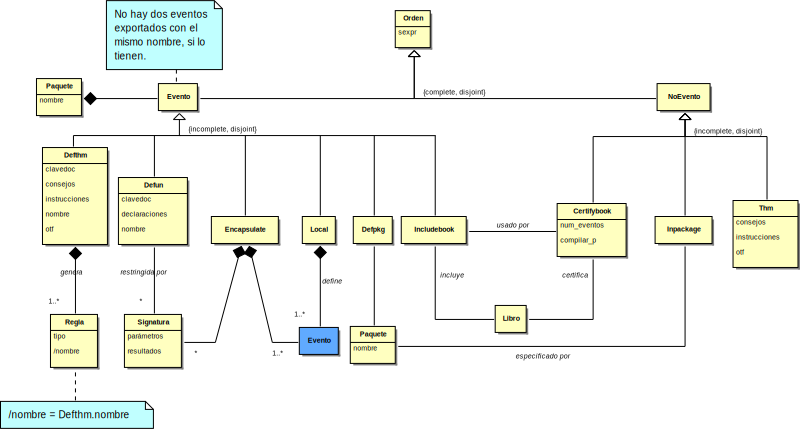
\includegraphics[width=\textwidth]{desarrollo/analisis/modacl2_ordenes}
  \caption{Diagrama de clases conceptuales de �rdenes de \acs{ACL2}}
  \label{fig:conceptual_ordenes}
\end{sidewaysfigure}

\begin{sidewaysfigure}
  \centering
  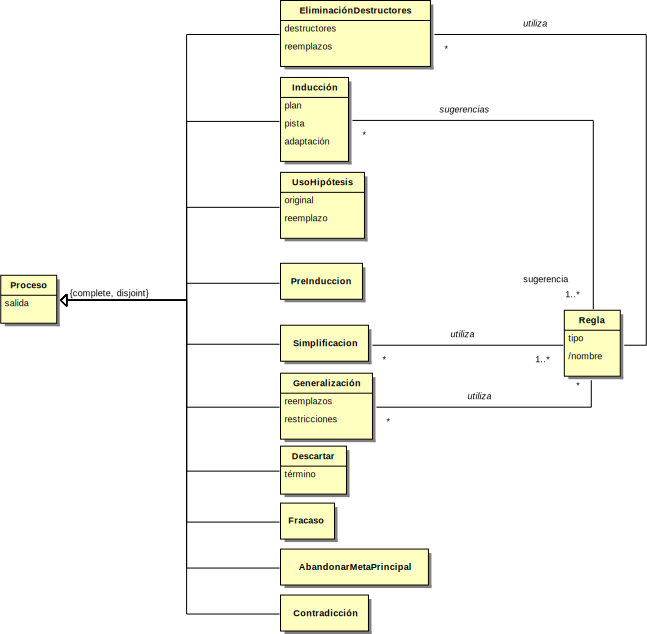
\includegraphics[height=.7\textheight]{desarrollo/analisis/modacl2_procesos}
  \caption{Diagrama de clases conceptuales de procesos de \acs{ACL2}}
  \label{fig:conceptual_procesos}
\end{sidewaysfigure}

\subsubsection{Restricciones textuales}

\begin{enumerate}
\item \emph{Clave externa}: ``nombre'' de \clase{Documento}.
\item \emph{Clave externa}: ``nombre'' de \clase{Paquete}.
\item \emph{Clave externa}: ``nombre'' de cualquier descendiente de
  \clase{Evento}, si lo tiene.
\item \emph{Clave externa}: ``clavedoc'' de cualquier descendiente de
  \clase{Evento}, si la tiene y est� especificada.
\item Todo \clase{Resultado} pertenece o a otro \clase{Resultado} o a una
  \clase{Demostraci�n}.
\item Todo \clase{Meta} pertenece o a otra \clase{Meta} o a un \clase{Resultado}.
\item Toda \clase{Meta} tiene una etiqueta �nica dentro de una \clase{Demostraci�n}.
\item \clase{Resultado}.�xito $\in{} \left\{ \text{verdadero},
    \text{falso} \right\}$.
\item \clase{Documento}.actualizado $\in{} \left\{ \text{verdadero},
    \text{falso} \right\}$.
\item \clase{Demostraci�n}.actualizada $\in{} \left\{ \text{verdadero},
    \text{falso} \right\}$.
\end{enumerate}

\subsubsection{Derivaciones}

\begin{enumerate}
\item \clase{Demostraci�n}.actualizada = ``verdadero'' si
  \clase{Demostraci�n}.fecha es una fecha y hora posterior a
  \clase{Enunciado}.fecha. ``falso'' de lo contrario.
\item \clase{Documento}.actualizado = ``verdadero'' si
  \clase{Demostraci�n}.actualizada y \clase{Documento}.fecha es una
  fecha y hora posterior a \clase{Demostraci�n}.fecha. ``falso'' de lo
  contrario.
\item \clase{Resultado}.�xito = no contiene \clase{Meta} con el
  \clase{Proceso} \clase{Fracaso} y sus \clase{Resultados} de inferior
  nivel (si los hay) tienen �xito.
\item \clase{Regla}.nombre = \clase{Defthm}.nombre.
\end{enumerate}

%%% Local Variables: 
%%% mode: latex
%%% TeX-master: "../../memoria"
%%% End: 


\subsection{Modelo conceptual de datos del dominio de \acs{YAML}}
\label{sec:datos_conceptual_yaml}
%
% Modelo conceptual de datos de YAML
% Copyright (C) 2008 Antonio Garc�a Dom�nguez
% $Id$
%

\subsubsection{Notaci�n}

Se seguir� la misma notaci�n que en~\S\ref{sec:conceptual_notacion}
(p�gina~\pageref{sec:conceptual_notacion}).

\subsubsection{Secuencia de procesado}
\label{sec:conceptual_yaml_general}

\index{YAML!flujo}
\index{YAML!operaciones}
\index{volcado|see{YAML!operaciones}}
\index{carga|see{YAML!operaciones}}

Toda implementaci�n de \ac{YAML} establece una correspondencia entre
las estructuras de datos nativas y los flujos de caracteres Unicode a
trav�s de una transformaci�n compuesta por tres pasos en cada
direcci�n, tal y como puede verse en la
figura~\ref{fig:secuenciaproc_yaml} de la
p�gina~\pageref{fig:secuenciaproc_yaml}. Los detalles de cada paso son
invisibles a los dem�s. Seg�n en qu� direcci�n nos desplacemos,
hablaremos de:

\begin{description}
\item[Volcado]

  Tomaremos una estructura de datos nativa del lenguaje de
  programaci�n y la presentaremos en forma de una sucesi�n de bytes
  dentro de un flujo. En la mayor�a de las implementaciones, esta
  operaci�n recibe el nombre de \verb#Dump#. Seguiremos estos pasos:

  \begin{enumerate}
  \item \emph{Representaci�n} de la estructura de datos nativa en
    forma de un grafo dirigido con ra�z, siguiendo el modelo de
    informaci�n de representaci�n de \ac{YAML} que describiremos
    posteriormente.

  \item \emph{Serializaci�n} del grafo a un �rbol de
    serializaci�n. Habr� que imponer un orden sobre los nodos del
    grafo, y evitar los problemas asociados con representar nodos con
    m�ltiples arcos entrantes y caminos con ciclos en un �rbol. Parte
    de estos detalles tambi�n aparecen en nuestro modelo conceptual de
    datos.

  \item \emph{Presentaci�n} en forma de una sucesi�n de bytes de la
    informaci�n del �rbol, recorri�ndolo para lanzar y despu�s
    capturar una serie de eventos de serializaci�n. Se emplear�n
    diversos estilos y notaciones para generar resultados f�cilmente
    legibles por humanos.
  \end{enumerate}

\item[Carga] 

  Este es el proceso inverso al volcado, y se suele encontrar bajo el
  nombre de \verb#Load#. Cada paso va descartando los detalles
  espec�ficos al paso correspondiente del volcado. Los pasos a seguir
  son:

  \begin{enumerate}
  \item \emph{An�lisis} de los bytes del flujo, lanzando y capturando
    los eventos de deserializaci�n correspondientes para producir el
    �rbol de serializaci�n que refleje la informaci�n original.

  \item \emph{Composici�n} del grafo de nodos a partir del �rbol,
    restableciendo los enlaces originales entre los nodos.

  \item \emph{Construcci�n} de las estructuras de datos nativas del
    lenguaje a partir del grafo de nodos.
  \end{enumerate}

\end{description}

\subsubsection{Modelos de informaci�n}
\label{sec:modinf_yaml}

\index{YAML!modelos de informaci�n}

Normalmente, las aplicaciones s�lo necesitan las estructuras de datos
finales, que se corresponden en muchos lenguajes (Perl, por ejemplo, o
Java, en menor grado) de manera bastante fiel a los grafos del modelo
de informaci�n de representaci�n. \yaxml{}, sin embargo, tiene unos
requisitos algo especiales: ha de asegurar una correspondencia entre
los grafos de \ac{YAML} y los �rboles de \ac{XML}, por lo que ha de
operar a un nivel menor de abstracci�n, utilizando el modelo de
informaci�n de serializaci�n descrito en~\cite{YAML}. Una adaptaci�n a
\ac{UML} de dicho modelo se halla en la
figura~\ref{fig:diaganalisis_yaml} de la
p�gina~\pageref{fig:diaganalisis_yaml}.

Explicaremos primero los elementos del modelo de informaci�n de
representaci�n de \ac{YAML}, y luego describiremos las modificaciones
que introduce el modelo de informaci�n de serializaci�n.

\paragraph{Modelo de informaci�n de representaci�n}

\index{YAML!documento}
\index{YAML!escalar}
\index{YAML!vector asociativo}
\index{YAML!secuencia}

Un documento \ac{YAML} se halla representado por el \clase{Nodo} ra�z
del grafo. Existen varias categor�as (\emph{kind} en el original) de
\clase{Nodo}s: \clase{Escalar}es que contienen una cadena opaca de
caracteres Unicode, \clase{Secuencia}s ordenadas de nodos, y vectores
asociativos (objetos de la clase \clase{VectorAsociativo}) que
contienen un conjunto no ordenado de pares clave-valor
(\clase{ParClaveValor}). Es interesante ver que tanto la clave como el
valor pueden ser nodos arbitrariamente complejos, pudiendo referirse
a cualquier otro nodo del grafo.

\index{forma can�nica|see{YAML!forma can�nica}}
\index{YAML!forma can�nica}

Todo nodo dispone de una etiqueta (\emph{tag} en el original) que
identifica el tipo abstracto de su contenido. Las etiquetas sirven
tambi�n en el caso de los escalares para unificar cadenas con el mismo
significado a una serie de formas can�nicas. Por ejemplo, las reglas
de la etiqueta \etiqueta{tag:yaml.org,2002:int} utilizan base 10 y un �nico
signo negativo opcional en sus formas can�nicas: un valor hexadecimal
como \verb#0xA# ser�a convertido por cualquier analizador al valor
decimal 10.

\index{YAML!ancla}
\index{YAML!alias}

\paragraph{Modelo de informaci�n de serializaci�n}

Modifica el modelo de representaci�n en dos aspectos:

\begin{enumerate}
\item A�ade un orden a los pares clave-valor de los vectores
  asociativos. Este orden es un detalle de serializaci�n, y no tiene
  impacto alguno en los grafos y estructuras de datos nativas
  generados.

\item Permite asociar a cualquier nodo un identificador o
  \emph{ancla}, y usar nodos \emph{alias} se�alando a esa ancla en
  posteriores referencias a ese nodo. Esto permite crear
  presentaciones compactas de grafos complejos, que podr�an incluso
  contener ciclos en su interior.

  Un ancla no tiene por qu� ser �nica: el nodo al que hace referencia
  un \emph{alias} no es m�s que el �ltimo que defini� esa ancla en el
  orden establecido.
\end{enumerate}

\begin{figure}
  \centering
  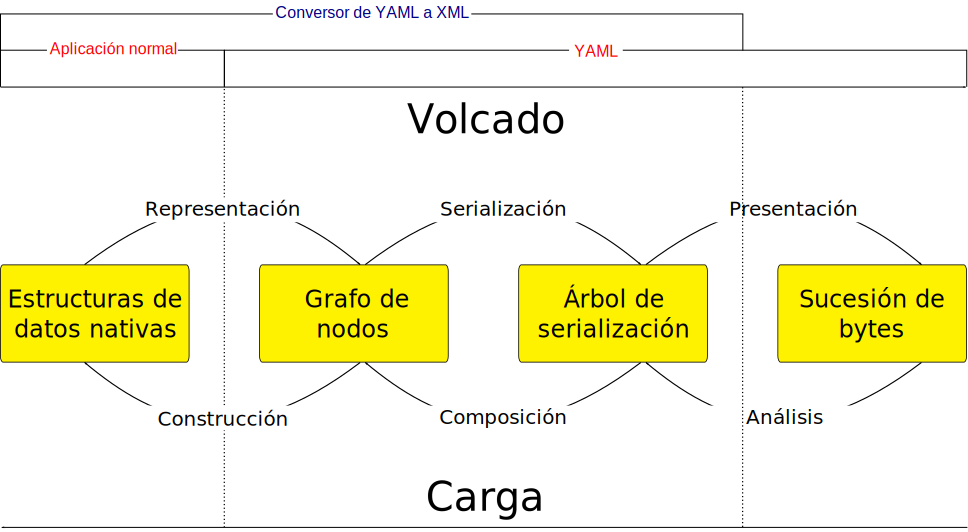
\includegraphics[width=\textwidth]{desarrollo/analisis/procesado_yaml}
  \caption{Secuencia de procesado de \acs{YAML}}
  \label{fig:secuenciaproc_yaml}
\end{figure}

\begin{sidewaysfigure}
  \centering
  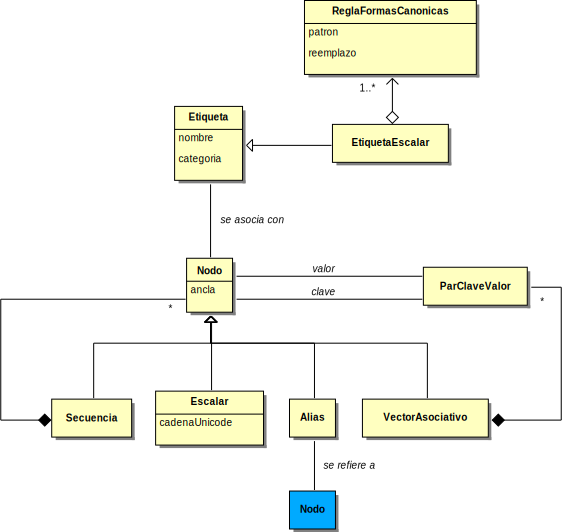
\includegraphics[height=.7\textwidth]{desarrollo/analisis/modyaml}
  \caption{Diagrama de clases conceptuales para \acs{YAML}}
  \label{fig:diaganalisis_yaml}
\end{sidewaysfigure}

\subsubsection{Restricciones textuales}
\label{sec:conceptual_yaml_restricciones}

\begin{itemize}
\item \emph{Clave externa}: ``nombre'' de Etiqueta.
\end{itemize}


%%% Local Variables: 
%%% mode: latex
%%% TeX-master: "../../memoria"
%%% End: 


%%% Local Variables: 
%%% mode: latex
%%% TeX-master: "../../memoria"
%%% End: 


\section{Dise�o del sistema}
\label{sec:diseno}
%%
%% Dise�o
%% Copyright (C) 2008 Antonio Garc�a Dom�nguez
%% $Id: diseno.tex 620 2008-07-01 23:20:02Z antonio $
%% 


\subsection{Arquitectura del sistema}
\label{sec:arquitectura}
%%
%% Arquitectura del sistema
%% Copyright (C) 2008 Antonio Garc�a Dom�nguez
%% $Id: arquitectura.tex 629 2008-07-06 13:47:58Z antonio $
%%

Para poder decidir la arquitectura del sistema, primero habr�a que
definir cu�les son las condiciones que afectar�n a su estructura.

Dichas condiciones se basan tanto en la funcionalidad esperada del
sistema, como en los requisitos no funcionales antes mencionados y
otros factores de calidad del software, como la flexibilidad,
mantenibilidad, reusabilidad o fiabilidad, entre otros.

La mantenibilidad requiere una arquitectura que evite la propagaci�n
de cambios realizados sobre una parte del sistema, definiendo
interfaces estables entre estas partes. Dicha arquitectura debe ser
adem�s lo m�s sencilla posible, para facilitar cambios en su
estructura y elementos.

La divisi�n en partes con l�mites e interfaces bien definidas mejora
tambi�n la reusabilidad y facilita las pruebas, evitando
acoplamientos innecesariamente complejos que dificulten el desarrollo
de una aplicaci�n fiable y con la funcionalidad deseada.

\subsubsection{Separaci�n de responsabilidades: divisi�n en capas}
\label{sec:arquitec_capas}
\index{patr�n arquitect�nico!Capas}
\index{Capas|see{patr�n arquitect�nico!Capas}}

En el caso de este proyecto, se deseaba separar \visor{} de los
detalles de los conversores externos, como \postprocesador{} y
\yaxml{}, y viceversa. En un futuro, se implementar�n nuevas
interfaces de usuario para \visor{}, por lo que tambi�n habr� que
separar la l�gica de aplicaci�n y de presentaci�n de \visor{}.

Bajo este contexto, se puede ver que la aplicaci�n del patr�n
arquitect�nico Capas (descrito con mayor detalle
en~\cite{archpatterns}) es natural. Se ha dividido la aplicaci�n en
cuatro capas:

\begin{description}
\item[Presentaci�n] 
  \index{capa!presentaci�n}

  Se ocupa de la interacci�n persona-m�quina en general y en
  particular de la visualizaci�n de la informaci�n y la navegaci�n a
  trav�s de �sta. Define las transformaciones a realizar sobre las
  representaciones creadas en la capa de filtrado.

\item[Aplicaci�n] 
  \index{capa!aplicaci�n}

  Responde a las peticiones de la capa superior, ejecut�ndolas de
  forma independiente a la interfaz escogida. Implementa la
  infraestructura necesaria para la ejecuci�n de las transformaciones
  de la capa de usuario, posibilitando su selecci�n en tiempo de
  ejecuci�n, enlazado de nodos y localizaci�n de cadenas. Incorpora la
  l�gica necesaria para la integraci�n con los conversores de la capa
  de filtrado.

\item[Filtrado] 
  \index{capa!filtrado}

  A diferencia de la usual capa de dominio en un modelo de tres capas,
  no manipula instancias de los objetos del dominio, sino que los
  transforma a una representaci�n manejable por las capas superiores,
  de ah� su nombre. 

  Se halla constituida por una serie de conversores independientes
  entre s� y de \visor{}, como \postprocesador{} o \yaxml{}. \visor{}
  s�lo ha de conocer la orden a ejecutar, que ha de seguir unas pautas
  muy sencillas:

  \begin{itemize}
  \item El c�digo de retorno de la orden debe indicar el �xito o
    fracaso en la conversi�n.
  \item El resultado \ac{XML} ha de volcarse por la salida est�ndar, y
    el estado de la conversi�n por la salida est�ndar de errores.
  \end{itemize}

\item[Servicios t�cnicos] 
  \index{capa!servicios t�cnicos}

  En esta capa hemos situado todas las bibliotecas, m�dulos externos y
  dem�s que proporcionan parte de la funcionalidad com�n del sistema,
  y son internos a �ste.

\end{description}

Se ha detallado la visi�n en capas (modeladas por paquetes \ac{UML}) a
lo largo del eje vertical y en particiones a lo largo del eje
horizontal en la figura~\ref{fig:arquitec_capas} de la
p�gina~\pageref{fig:arquitec_capas}.

M�s tarde examinaremos cada una de estas capas por separado.

\begin{figure}
  \centering
  \includegraphics[width=.8\textwidth]{desarrollo/diseno/arquitec_capas}
  \caption{Diagrama arquitect�nico del sistema}
  \label{fig:arquitec_capas}
\end{figure}

\subsubsection{Transformaciones configurables: tuber�as y filtros}
\label{sec:tuberias_filtros}
\index{patr�n arquitect�nico!Tuber�as y Filtros}
\index{Tuber�as y Filtros|see{patr�n arquitect�nico!Tuber�as y
    Filtros}}

\paragraph{Descripci�n}

Otro patr�n arquitect�nico usado (con ciertas licencias) en el dise�o
de este proyecto fue Tuber�as y Filtros. Dicho patr�n ser� familiar a
todo usuario de un sistema UNIX, de donde se inspir� precisamente.

Consiste en el encadenamiento de una serie de Filtros, partiendo de
una Fuente de informaci�n, y llegando hasta un Sumidero, destino de la
informaci�n transformada. A cada paso, la informaci�n llega a un
Filtro a trav�s de una Tuber�a, saliendo por otra Tuber�a hacia el
siguiente Filtro o el Sumidero final.

El patr�n original (ver~\cite{archpatterns}) tiene las ventajas de ser
f�cilmente paralelizable en filtros incrementales que no necesiten
leer toda la entrada antes de poder operar, y permitir una gran
flexibilidad cambiando el filtro exacto usado a cada paso, dado que
est�n dise�ados para ser intercambiables entre s�, con ciertas
limitaciones.

Sus desventajas consisten en la dificultad de mantener un estado
compartido y de realizar un control detallado de errores, al ser
usualmente tratada toda la transformaci�n como una unidad.

\paragraph{Uso}

El uso de este patr�n a lo largo de este proyecto se fundament� en la
necesidad de permitir la extensibilidad de la visualizaci�n por parte
del usuario sin necesidad de una recompilaci�n, usando un enfoque
puramente dirigido por datos.

As�, en el caso de una demostraci�n de \ac{ACL2}, si consideramos al
sistema externo \ac{ACL2} como la fuente de la informaci�n y a la
visualizaci�n por parte de la biblioteca Swing como el sumidero,
tendr�amos cuatro filtros intermedios:

\begin{enumerate}
\item \postprocesador{}, con el enunciado Lisp para \ac{ACL2} como
  entrada, genera una representaci�n en \ac{XML} del contenido de la
  demostraci�n realizada. El formato de salida se conoce a trav�s de
  una \ac{DTD}, incrustada en el propio documento de salida.

\item El segundo filtro, definido en la capa de presentaci�n, realiza
  una transformaci�n previa, potencialmente costosa, que afecta a todo
  el documento, y que s�lo se realiza una vez.
  
  Aqu� el usuario puede definir el aspecto que tendr� el �rbol del
  documento, ocultando nodos o cambiando la etiqueta o icono a
  mostrar. La descripci�n de la hoja define las entradas esperadas y
  el formato de la salida.

\item El tercer filtro, tambi�n en la capa de presentaci�n, transforma
  un nodo a su visualizaci�n \ac{XHTML} utilizando una hoja \ac{XSLT}
  para el formato de la salida. La transformaci�n se repite cada vez
  que el usuario cambia de nodo.

  En este caso, se sabe que la salida es \ac{XHTML}, y que sigue por
  lo tanto una \ac{DTD} conocida. Tambi�n podemos deducir a partir del
  nombre de la hoja qu� entrada espera y qu� salida produce.

  As�, sabemos que la hoja \fichero{ppACL2} de visualizaci�n tomar� la
  salida de la hoja de preprocesado \fichero{ppACL2} o una derivada
  suya y mostrar� la informaci�n relevante a demostraciones de
  \ac{ACL2} contenida en dicho documento.

  Una hoja de visualizaci�n es dise�ada suponiendo que la salida del
  preprocesado sigue el formato de salida de ciertas hojas de usuario
  de preprocesado. En el caso contrario, la transformaci�n no fallar�,
  pero no se obtendr�n los resultados esperados.

\item El cuarto filtro, controlado por la capa de aplicaci�n, marca
  las coincidencias de la clave de la b�squeda en curso en el texto,
  si se da el caso. Tambi�n se aplica una hoja de estilos \ac{CSS},
  que no modifica la estructura pero s� el aspecto del resultado
  final.

\end{enumerate}

Como vemos, los dos filtros intermedios se ocupan de la mayor parte de
la visualizaci�n, y seg�n los requisitos funcionales, �stos deber�an
ser modificables por el usuario sin necesidad de recompilaci�n.

\paragraph{Implementaci�n}

\index{XSLT!ventajas}

Se eligi� \ac{XSLT} para implementar estos dos filtros por la
flexibilidad que ofrece al estar basado en ficheros de texto
f�cilmente intercambiables y por su capacidad de describir
declarativamente las transformaciones sobre la fuente \ac{XML} a otros
formatos.

Se opt� por una visualizaci�n basada en \ac{XHTML} para evitar el uso
de numerosos componentes discretos Swing, complicando el dise�o de la
interfaz y las extensiones por parte del usuario. El uso de hipertexto
permite, adem�s de ofrecer mayor informaci�n visual al usuario,
establecer enlaces entre los distintos elementos de la
demostraci�n.

Existen varias diferencias con el patr�n original. Los filtros aqu�
usados no son incrementales (el uso de \ac{XML} no lo permite),
perdi�ndose la capacidad de paralelizaci�n.

Por otro lado, la p�rdida de capacidad de detecci�n detallada de
errores no aparece en nuestro caso, al basarse las tuber�as en l�gica
de la capa de aplicaci�n y no en otros mecanismos de menor nivel de
abstracci�n, como memoria compartida.

No ha sido necesario ning�n estado compartido, por lo que esta otra
desventaja tampoco ha resultado ser ninguna limitaci�n.

\index{translet}

En cuanto a rendimiento, hay que considerar el uso de \emph{translets}
por el procesador \ac{XSLT} Xalan XSLTC. �stos son representaciones
compiladas a bytecode Java de hojas \ac{XSLT} cuya ejecuci�n es
notablemente m�s r�pida que la ejecuci�n interpretada cl�sica, a costa
de cierta funcionalidad innecesaria para este proyecto.

La disposici�n e interconexi�n de los componentes que intervienen en
la transformaci�n se ha recogido en el diagrama \ac{UML} de
componentes de la figura~\ref{fig:componentes_filtros} de la
p�gina~\pageref{fig:componentes_filtros}.

La capa de aplicaci�n no aparece en �l, pero se halla impl�cita, como
capa de control. Tampoco han de confundirse las hojas \ac{XSLT}
usadas, que pertenecen a la capa de presentaci�n, con su l�gica de
control, parte de la capa de aplicaci�n.

\begin{figure}
  \centering
  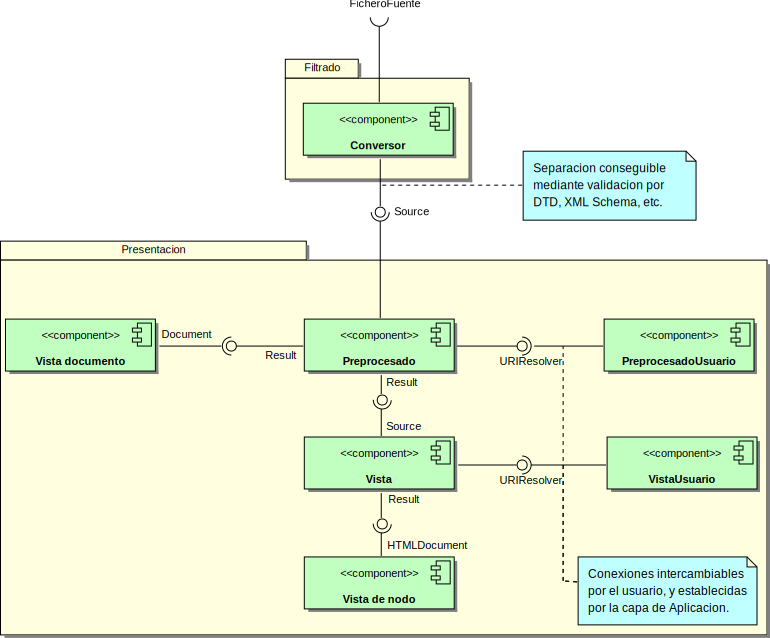
\includegraphics[width=\textwidth]{desarrollo/diseno/componentes}
  \caption{Diagrama de componentes para visualizaci�n}
  \label{fig:componentes_filtros}
\end{figure}

\subsubsection{Integraci�n de las capas de aplicaci�n y presentaci�n: patrones \acs{MVP}}
\label{sec:arquitectura_mvp}

\index{patr�n arquitect�nico!MVC}
\index{patr�n arquitect�nico!MVP}
\index{patr�n arquitect�nico!Controlador Supervisor}
\index{patr�n arquitect�nico!Vista Pasiva}
\index{patr�n arquitect�nico!Modelo de Presentaci�n}
\index{MVC|see{patr�n arquitect�nico!MVC}}
\index{MVP|see{patr�n arquitect�nico!MVP}}
\index{Controlador Supervisor|see{patr�n arquitect�nico!Controlador Supervisor}}
\index{Vista Pasiva|see{patr�n arquitect�nico!Vista Pasiva}}
\index{Modelo de Presentaci�n|see{patr�n arquitect�nico!Modelo de Presentaci�n}}

En el visor del Proyecto que precede a �ste, se hab�a establecido una
comunicaci�n entre las capas de aplicaci�n y de presentaci�n mediante
Fachadas. Estas Fachadas constitu�an el �nico punto de acceso a la
funcionalidad de cada capa, y evitaban que la capa superior tuviera
que conocer los detalles de la capa inferior.

Aunque para sistemas con interfaces m�s sencillos se podr�a haber
continuado su uso, en el caso de \visor{} se vio c�mo las Fachadas
iban tomando demasiadas responsabilidades al mismo tiempo. Tambi�n se
dio el caso de que la capa inferior forzaba a la capa superior a una
serie de restricciones, siendo la m�s grave la de tratar un �nico
documento.

Otro problema que aquejaba al antiguo dise�o es la pr�cticamente nula
capacidad para poder realizar pruebas de unidad de forma c�moda en la
aplicaci�n. Existen herramientas que permiten automatizar pulsaciones
y entrada de teclado, pero las pruebas de este tipo son extremadamente
fr�giles: cualquier cambio en la disposici�n de los controles de la
interfaz las invalidar�a.

Para resolver ambos problemas, se estudiaron las diversas alternativas
ofrecidas en~\cite{Fowler:GUIArch}, y en particular las derivaciones
del patr�n \ac{MVP}. Este patr�n es una derivaci�n del
\ac{MVC}~\cite{gof} original en el que en vez de tener un tr�o
modelo-vista-controlador para cada control de la interfaz (como un
campo de texto, por ejemplo), tenemos un tr�o para el formulario
completo. Ahora el modelo del formulario es el conjunto de clases del
dominio usadas, la vista es la estructura formada por todos los
controles gr�ficos del formulario, y el presentador es el componente
al que se notifican todas las acciones de inter�s realizadas por el
usuario.

El presentador es el ocupado de modificar el modelo, y posteriormente
la vista se actualizar� con los cambios hechos por el presentador al
modelo. Hay diversos mecanismos para garantizar esta sincronizaci�n,
constituyendo variantes distintas del patr�n \ac{MVP} b�sico:

\begin{description}
\item[Controlador Supervisor] Para los casos simples, la
  sincronizaci�n modelo-vista se establece a partir del patr�n
  Observador o alg�n otro enfoque declarativo. En casos m�s complejos,
  el presentador interviene directamente sobre los controles de la
  interfaz.

\item[Vista Pasiva] La vista en este caso carece de cualquier l�gica
  de sincronizaci�n, y es el presentador el que rellena todos los
  campos. Una posibilidad para evitar acoplar demasiado el presentador
  a los controles usados es definir una interfaz en el formulario para
  su relleno: de esta forma, durante las pruebas de unidad podemos
  sustituir la vista por un Doble para Pruebas~\cite{Meszaros:XUnit} y
  depurar pr�cticamente toda la funcionalidad.

\item[Modelo de Presentaci�n] El presentador contiene el estado
  abstracto que deber�a presentar el formulario. Puede que sea el
  modelo de presentaci�n el que manipule la vista, o que sea la vista
  la que se actualice a partir del modelo de presentaci�n. En el
  primer caso, ambos elementos est�n m�s acoplados pero podemos probar
  la sincronizaci�n. En el segundo caso, la sincronizaci�n no se puede
  depurar tan f�cilmente, pero el modelo de presentaci�n es
  completamente independiente de la interfaz usada.

\end{description}

De entre estos enfoques, se escogi� el Modelo de Presentaci�n, ya que
en un futuro se desean crear nuevas interfaces para \visor{}: el
presentador no deber�a de saber nada acerca de la vista. Por la misma
raz�n, es la vista la que se actualiza al estado encapsulado por el
modelo de presentaci�n.

El uso de un modelo de presentaci�n tambi�n facilita la implementaci�n
de una interfaz multidocumento: cada documento puede imponer su propio
estado de presentaci�n sin afectar a los dem�s.

En cuanto a la divisi�n en modelo-vista-presentador, tendr�amos a los
modelos y otros servicios de alto nivel en la capa de aplicaci�n, y a
las vistas y presentadores en la capa de presentaci�n.

%%% Local Variables: 
%%% mode: latex
%%% TeX-master: "../../memoria"
%%% End: 


\subsection{Capa de filtrado: \nombrepostprocesador{}}
\label{sec:capa_filtrado_acl2}
%%
%% Capa de filtrado: ACL2
%% Copyright (C) 2008 Antonio Garc�a Dom�nguez
%% $Id: capa_filtrado_acl2.tex 629 2008-07-06 13:47:58Z antonio $
%%

Volviendo al diagrama de capas de la figura~\ref{fig:arquitec_capas}
de la p�gina~\pageref{fig:arquitec_capas}, vemos que este conversor ha
de:
\begin{itemize}
\item Convertir la salida de \ac{ACL2} a \ac{XML} sin p�rdidas.
\item Definir claramente el formato de dicha salida.
\end{itemize}

Por la necesidad de manipular el texto de la forma m�s sencilla y
potente posible, se escogi� usar un gui�n escrito en Perl, un lenguaje
dise�ado a este efecto.

A ra�z de la complejidad inherente en el manejo de la salida en
lenguaje humano de un programa como \ac{ACL2}, se ha seguido el
paradigma orientado a objetos a la hora de desarrollar
\postprocesador{}.

\subsubsection{Procesado general de proyectos de \acs{ACL2}}
\label{sec:postproc_estruc_general}

El dise�o b�sico se fundamenta en el modelo conceptual de datos, con
ciertas modificaciones. El gui�n lanzado por la capa de aplicaci�n
emplea la funci�n \funcion{convertir\_a\_xml} del m�dulo
\clase{Procesador}, pas�ndole la ruta al \clase{Enunciado} ra�z del
proyecto completo, y vuelca sus resultados por la salida est�ndar.

Este m�todo es realmente un envoltorio que crea un \clase{Proyecto}
con ra�z en el \clase{Enunciado} indicado, actualiza por completo de
forma recursiva todas las salidas de \ac{ACL2} y sus versiones en
\ac{XML} y devuelve la versi�n \ac{XML} de la salida de la ra�z del
proyecto.

Las \clase{Dependencias} del \clase{Proyecto} son obtenidas a partir
de un an�lisis est�tico del c�digo Lisp, empezando por el
\clase{Enunciado} Lisp ra�z y continuando de forma recursiva. Esto
genera un �rbol anidado de \clase{Proyecto}s que dependen unos de
otros. Decimos �rbol y no grafo pues un subproyecto puede aparecer
varias veces en el mismo �rbol. Esto supone un coste mayor en espacio,
pero no en tiempo: si tuviera que ser actualizado, s�lo ser�a
procesado una vez. Se est�n considerando representaciones m�s
eficientes en espacio para versiones posteriores.

El proceso de actualizaci�n consiste en recorrer el �rbol e ir
actualizando de forma recursiva:

\begin{enumerate}
\item Se solicita la actualizaci�n de las \clase{Dependencias} del
  proyecto actual, que forman \clase{Proyecto}s a su vez.

\item Si alg�n subproyecto fue actualizado o el fichero temporal con
  la salida de \ac{ACL2} no existe o tiene una fecha de modificaci�n
  m�s antigua que la del \clase{Enunciado}, se invocar� a \ac{ACL2}
  para crear o actualizar dicho fichero temporal.

\item Si el fichero temporal con la salida fue actualizado o el
  fichero temporal con el documento \ac{XML} resultante no existe o
  tiene una fecha de modificaci�n m�s antigua que la de la salida, se
  actualizar� empleando una instancia de la clase
  \clase{Demostraci�n}, que encapsula el proceso de an�lisis de una
  demostraci�n de \ac{ACL2}.
\end{enumerate}

El diagrama de secuencia correspondiente a esta l�gica se halla en el
cuadro~\ref{fig:ds_filtrado_general} de la
p�gina~\pageref{fig:ds_filtrado_general}. El diagrama con las clases
participantes, integradas con las ocupadas de procesar las
\clase{Demostracion}es en s�, forma el
cuadro~\ref{fig:diag_clases_diseno_pproc} de la
p�gina~\pageref{fig:diag_clases_diseno_pproc}.

\begin{sidewaysfigure}
  \centering
  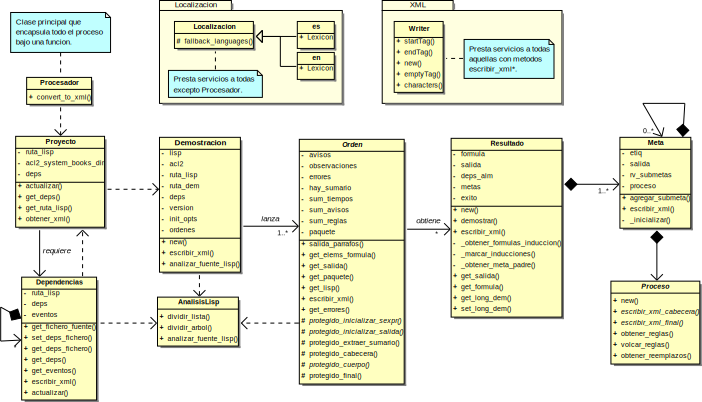
\includegraphics[width=\textwidth]{desarrollo/diseno/clases_acl2proc_general}
  \caption{Diagrama de clases de \postprocesador{} (general)}
  \label{fig:diag_clases_diseno_pproc}
\end{sidewaysfigure}

\begin{sidewaysfigure}
  \centering
  \includegraphics[width=\textwidth]{desarrollo/diseno/diag_sec_acl2proc_general}
  \caption{Diagrama de secuencia general de filtrado}
  \label{fig:ds_filtrado_general}
\end{sidewaysfigure}

\subsubsection{Generaci�n de modelos en memoria}

Un concepto importante para comprender el dise�o de \postprocesador{}
en esta versi�n es la necesidad cada vez mayor de atrasar el momento
de la generaci�n de la salida \ac{XML}. Originalmente, ambos estaban
intercalados. Sin embargo, en muchos casos el orden en que se procesa
la informaci�n no coincide con el orden en que se debe producir la
salida, y esto supon�a un impedimento para el procesamiento de
demostraciones cada vez m�s complejas.

A lo largo de las iteraciones, se ha hecho una divisi�n mayor y mayor,
hasta finalmente separar el procesado y la salida a nivel de una
\clase{Demostraci�n} completa, en vez de \clase{Resultado}s
individuales.  Esto permite dar nuevos usos al an�lisis ya
implementado. Puede verse esta separaci�n en el diagrama de secuencia
de la figura~\ref{fig:ds_filtrado_demo} de la
p�gina~\pageref{fig:ds_filtrado_demo}: la inicializaci�n se hace s�lo
durante la ejecuci�n del constructor \metodo{new}, y la salida se
produce exclusivamente dentro del m�todo \metodo{escribir\_xml}.

Por ejemplo, se puede analizar una \clase{Demostraci�n} sin contar con
su salida, realizando un an�lisis est�tico sobre el c�digo Lisp: toda
\clase{Orden} dispone de m�todos separados para recuperar informaci�n
de la S-expresi�n y de la salida de \ac{ACL2}, y el �ltimo s�lo es
usado cuando se proporciona dicha salida en el constructor. Este
an�lisis est�tico proporciona informaci�n de todas las dependencias de
un proyecto.

\begin{sidewaysfigure}
  \centering
  \includegraphics[width=.8\textwidth]{desarrollo/diseno/diag_sec_acl2proc_demostracion}
  \caption{Diagrama de secuencia de filtrado de una \clase{Demostraci�n}}
  \label{fig:ds_filtrado_demo}
\end{sidewaysfigure}

\subsubsection{Relaci�n con capa de servicios t�cnicos}
\label{sec:postproc_servtecnicos}
\index{�rbol Perl}

Viendo el diagrama general de clases de dise�o para la capa de
filtrado, se puede observar que la mayor�a de las clases tienen
dependencias con \clase{XML::Writer} y \clase{Localizaci�n}.

Esto es lo usual con los elementos de la capa de servicios t�cnicos:
\clase{XML::Writer} es un m�dulo usado para la salida \ac{XML}, que
incorpora ciertas comprobaciones autom�ticas para garantizar la
ejecuci�n de generaci�n de documentos bien formados, y
\clase{Localizaci�n} es el m�dulo usado para localizaci�n de mensajes
de error o avisos.

No hay que confundir dichos servicios t�cnicos con clases de utilidad
como \clase{An�lisisLisp}, que a�sla la l�gica necesaria para
convertir listas y �rboles Lisp a estructuras de datos equivalentes de
Perl.

\subsubsection{Reflexi�n y tipos basados en comportamiento:
  simplificaci�n del an�lisis est�tico}
\label{sec:acl2proc_reflexion}

Al implementar el an�lisis est�tico necesario para conseguir el grafo
de dependencias de un proyecto, surge la necesidad de conocer cu�l
ser�a el identificador final y paquete de cada evento, y de las rutas
de todos los libros. Evidentemente, hay que distinguir entre los
\clase{Evento}s con nombre, los \clase{Evento}s sin nombre y los
\clase{NoEvento}s, que no producen cambios en el mundo l�gico de
\ac{ACL2}.

Sin embargo, se desea conservar toda la l�gica propia a cada orden en
su propia subclase de \clase{Orden}. La forma m�s l�gica ser�a a�adir
niveles a la estructura de herencia, distinguiendo as� entre los
\clase{Evento}s con nombre, los \clase{Evento}s sin nombre y los
\clase{NoEvento}s, pero esto s�lo resolver�a parte del problema:
seguir�amos teniendo que preguntar si la \clase{Orden} usada pertenece
a la lista de aquellas que afectan al paquete actual, o de la lista de
\clase{Orden}es ocupadas del manejo de libros. Tendr�amos entonces que
utilizar herencia m�ltiple. Como vemos, preguntar por la subclase
exacta de la \clase{Orden} seg�n el criterio que necesitemos en un
momento determinado a�ade una complejidad al c�digo y crea un
acoplamiento mucho mayor de lo esperado.

\index{duck typing}

La alternativa se halla en el concepto conocido como ``duck
typing''~\cite{Martelli2000}, muy popular en lenguajes con sistemas de
tipos din�micos como Python, y defendido (aunque no bajo ese mismo
nombre) por autores como Bruce Eckel~\cite{EckelDuckTyping}. La
definici�n del glosario de Python~\cite{DuckTyping} es la siguiente:

\begin{quotation}
  Pythonic programming style that determines an object's type by
  inspection of its method or attribute signature rather than by
  explicit relationship to some type object ("If it looks like a duck
  and quacks like a duck, it must be a duck.") By emphasizing
  interfaces rather than specific types, well-designed code improves
  its flexibility by allowing polymorphic substitution. Duck-typing
  avoids tests using type() or isinstance(). Instead, it typically
  employs hasattr() tests or EAFP programming.
\end{quotation}

Es decir, no distinguimos a los tipos por ``qui�nes'' son, con
\verb#instanceof# en Java o \verb#typeid# en \CPP, por ejemplo, y
luego hacemos \emph{upcasting} a una clase o interfaz com�n. En su
lugar, los distinguimos por c�mo se comportan: si \verb#anda()# como
un \clase{Pato} y \verb#hace_cuac()# como un \clase{Pato}, entonces es
un \clase{Pato} para nuestro c�digo.

Se podr�a ver el ``duck typing'' como una versi�n de la programaci�n
gen�rica de \CPP en que la comprobaci�n de tipos se hace en tiempo de
ejecuci�n y s�lo se requieren aquellos m�todos que son realmente
usados, en vez de todos las que aparecen en el c�digo.

\index{EAFP}

Existen dos estilos para su implementaci�n, como sugiere la definici�n
anterior. El segundo estilo hace referencia al acr�nimo \ac{EAFP}:
asumimos que los m�todos necesarios se implementan y capturamos los
errores si nos equivocamos. Dado que en el an�lisis est�tico se
mezclan las \clase{Orden}es que cumplen o no cada uno de los criterios
libremente, este m�todo no nos sirve: el manejo de excepciones no es
un mecanismo de control de flujo, al fin y al cabo.

\index{reflexi�n}

El primer m�todo s� es �til, pero notemos que hace uso de algo que no
todo lenguaje tiene: la capacidad de consultar y operar sobre la
propia estructura del programa, en tiempo de ejecuci�n. Dicho proceso
es conocido como \emph{reflexi�n}, y se halla integrado dentro de
muchos lenguajes, como Java, C\#, Perl o Python.

As�, el an�lisis est�tico asume que si una clase implementa el m�todo
\metodo{get\_nombre\_paquete} cambia el paquete actual, si implementa
\metodo{get\_identificador\_evento} representa a un \clase{Evento} con
un nombre referenciable posteriormente, y si implementa el m�todo
\metodo{get\_ruta\_libro}, que de alguna forma ha incluido los
contenidos del libro bajo la ruta especificada bajo el mundo l�gico de
\ac{ACL2}.

\subsubsection{Patr�n M�todo F�brica: creaci�n de �rdenes y Procesos}
\label{sec:postproc_patron_fabrica}
\index{patr�n de dise�o!M�todo F�brica}
\index{M�todo F�brica|see{patr�n de dise�o!M�todo F�brica}}

Se us� el patr�n \patron{M�todo F�brica} de~\cite{gof} para aislar
al resto del post-procesador de la l�gica necesaria para identificar
qu� tipo de \clase{Orden} o \clase{Proceso} hay que crear exactamente.

Podemos ver en el diagrama de clases de dise�o general de la
figura~\ref{fig:diag_clases_diseno_pproc} en la
p�gina~\pageref{fig:diag_clases_diseno_pproc} dos clases abstractas,
\clase{Orden} y \clase{Proceso}. Las instancias de sus subclases se
crean mediante los m�todos \metodo{crear} de
\clase{ACL2::Orden::Fabrica} y \clase{ACL2::Proceso::Fabrica}.

\index{paquete Lisp}

En ambos casos, son los valores de los argumentos proporcionados los
que determinan qu� subclase concreta de la clase abstracta base se va
a crear. En el caso de \clase{Orden}, se env�a la S-expresi�n, el
paquete Lisp actual y la salida. En el caso de \clase{Proceso}, se
env�a la salida.

\clase{ACL2::Proceso::Fabrica} requiere algo m�s de participaci�n por
parte de las subclases de Proceso. Todas deben registrar una subrutina
an�nima que determine si la salida enviada por \clase{Meta} se
corresponde con ella, y que devuelva los par�metros requeridos al
constructor en dicho caso. Esto podr�a considerarse como un uso del
patr�n \patron{Orden}, descrito en m�s detalle en la capa de
presentaci�n.

Dicha f�brica queda as� como un punto central f�cilmente accesible por
\clase{Meta} de creaci�n de \clase{Proceso}s, y la l�gica espec�fica a
cada proceso se halla concentrada y separada del resto en un �nico
fichero.


\subsubsection{Patr�n M�todo Plantilla}
\label{sec:postproc_patron_metplantilla}
\index{patr�n de dise�o!M�todo Plantilla}
\index{M�todo Plantilla|see{patr�n de dise�o!M�todo Plantilla}}
\index{operaciones de enganche}

Este patr�n, tambi�n proveniente de~\cite{gof}, se usa en la jerarqu�a
de \clase{Orden} para reunir todo el comportamiento com�n en el
filtrado de las �rdenes.

Toda orden en \ac{ACL2} produce una serie de mensajes de error, aviso
u observaci�n. Tambi�n se a�ade usualmente (pero no siempre) un
sumario, cuyo formato es fijo en toda orden. Se da adem�s que la
l�gica de manejo de errores de \ac{ACL2} es siempre la misma.

Toda esta l�gica com�n es reunida en un m�todo de una clase base, que
emplea una serie de ``operaciones de enganche'' protegidas, que
permiten especializar mediante herencia partes de ese m�todo con la
l�gica espec�fica para cada orden, facilitando a�adir nuevas �rdenes o
modificar las existentes. El nombre de ``m�todo plantilla'' viene de
esa capacidad de rellenar los ``huecos'' de su l�gica.

\clase{Orden} dispone de dos m�todos plantilla:

\begin{enumerate}
\item \metodo{inicializar} dispone de los enganches:
  \begin{itemize}
  \item \metodo{protegido\_inicializar\_sexpr}: operaci�n abstracta.
  \item \metodo{protegido\_inicializar\_salida}: operaci�n abstracta.
  \item \metodo{protegido\_extraer\_sumario}: tiene una implementaci�n
    por defecto.
  \end{itemize}

\item \metodo{escribir\_xml} se puede especializar a partir de:

  \begin{itemize}
  \item \metodo{protegido\_cabecera}: tiene una implementaci�n por
    defecto.
  \item \metodo{protegido\_cuerpo}: operaci�n abstracta.
  \item \metodo{protegido\_final}: tiene una implementaci�n por
    defecto.
  \end{itemize}
\end{enumerate}

El uso del prefijo ``\metodo{protegido\_}'' en los nombres se trata de
un esquema de nombrado, siguiendo la pr�ctica com�n en muchos m�dulos
del \ac{CPAN}, y no implica la existencia de un mecanismo de control
de acceso real, por sencillez.

\subsubsection{Jerarqu�a de �rdenes}
\label{sec:postproc_jerarq_ordenes}

El diagrama de clases de dise�o \ac{UML} puede verse en la
figura~\ref{fig:postproc_jerarq_ordenes} de la
p�gina~\pageref{fig:postproc_jerarq_ordenes}.

Puede verse como cada clase redefine los m�todos de enganche
necesarios, a�adiendo algunas operaciones privadas para su propia
funcionalidad.

\begin{figure}
  \centering
  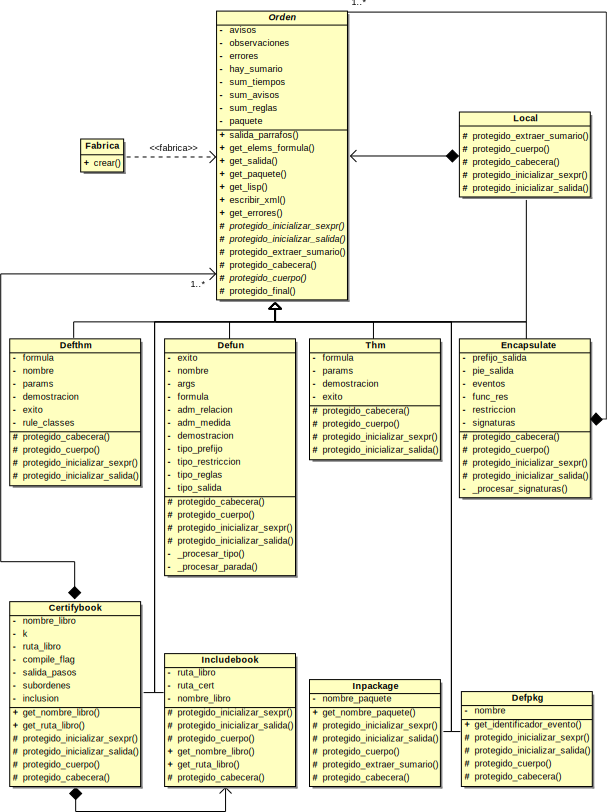
\includegraphics[width=\textwidth]{desarrollo/diseno/clases_acl2proc_ordenes}
  \caption{Diagrama de clases de �rdenes de \postprocesador{}}
  \label{fig:postproc_jerarq_ordenes}
\end{figure}

\subsubsection{Jerarqu�a de Procesos}
\label{sec:postproc_jerarq_procesos}

El diagrama de esta jerarqu�a se halla en la
figura~\ref{fig:postproc_jerarq_procesos} de la
p�gina~\pageref{fig:postproc_jerarq_procesos}.

Los m�todos privados est�ticos \metodo{\_identificar} contienen el
c�digo que se registra en la \clase{F�brica}, utilizando una subrutina
an�nima (parecida a una clausura lambda). Para ocultar los detalles,
\clase{F�brica} emula en su m�todo \metodo{registrar} control de
acceso por paquete.

\begin{figure}
  \centering
  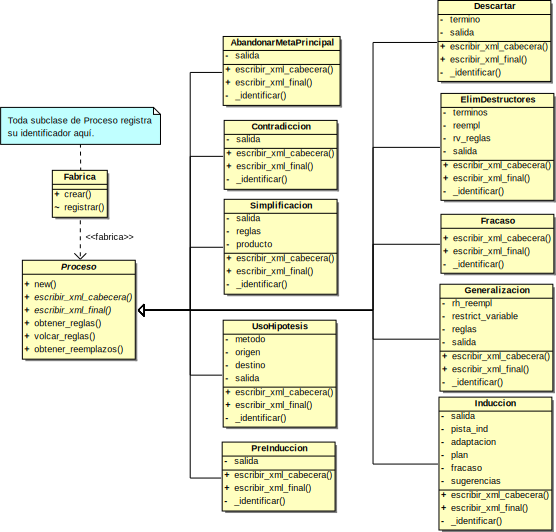
\includegraphics[width=\textwidth]{desarrollo/diseno/clases_acl2proc_procesos}
  \caption{Diagrama de clases de Procesos de \postprocesador{}}
  \label{fig:postproc_jerarq_procesos}
\end{figure}

\subsubsection{Un ejemplo: definici�n de teorema}
\label{sec:postproc_ejemplo_defthm}

Para explicar en m�s detalle qu� es lo que se requiere para el
filtrado de una orden de \ac{ACL2}, usaremos como ejemplo el procesado
de un supuesto evento de definici�n de un teorema, \texttt{defthm}.

\index{patr�n de dise�o!F�brica Abstracta}

Tras crearse la \clase{Orden} a trav�s de la \patron{F�brica
  Abstracta} \clase{Orden::Fabrica}, se generar� la versi�n \ac{XML}
de la salida de \ac{ACL2} en dos pasos. Cada paso se corresponde con
uno de los m�todos plantilla antes mencionados.

En primer lugar, se captura toda la informaci�n disponible en la
salida de \ac{ACL2} (si se proporciona) y la S-expresi�n original
mediante \metodo{inicializar}:

\begin{enumerate}
\item \metodo{\_init\_desde\_salida} definido por \clase{Orden} retira
  toda la informaci�n de la salida no espec�fica a la \clase{Orden}
  \clase{Defthm}, simplificando as� su inicializaci�n.

  Ello incluye retirar los mensajes de \ac{ACL2}, los mensajes del
  colector de basura del int�rprete Lisp y el sumario de la ejecuci�n
  de la orden.

\item \metodo{protegido\_inicializar\_sexpr}, propio de
  \clase{Defthm}, obtiene informaci�n espec�fica a \clase{Defthm} a
  partir de su S-expresi�n:

  \begin{itemize}
  \item F�rmula a demostrar.

  \item Nombre del teorema.

  \item Clases de regla a generar, con el valor por defecto
    ``:REWRITE'', indicando que se usar� una regla de reescritura de
    miembros.

  \item Activaci�n o desactivaci�n de la bandera OTF (``on through the
    fog''), obligando a \ac{ACL2} a que, si con s�lo simplificar no
    basta, no intente inducir sobre la f�rmula original, sino sobre
    las m�ltiples f�rmulas resultantes de las simplificaciones.

  \item Captura de otros argumentos de inter�s.
  \end{itemize}

\item \metodo{protegido\_inicializar\_salida}, definido por
  \clase{Defthm}, se ocupa de recabar toda la informaci�n de inter�s
  del texto de la salida de \ac{ACL2}. Nos interesan las dependencias
  de almacenamiento de las reglas generadas, y los pasos de la
  demostraci�n realizada.

  En primer lugar, recuperaremos la informaci�n mediante el m�todo
  plantilla \metodo{inicializar}:

  \begin{enumerate}
  \item Obtener cada una de las metas e inicializarlas. Tras dividir
    la salida completa en la salida de cada meta, se emplear� el
    \patron{M�todo F�brica} \metodo{crear} de
    \clase{Proceso::Fabrica}, que invocar� a las subrutinas an�nimas
    registradas para reconocer e instanciar el \clase{Proceso} exacto
    seguido.

    Cada meta introducida se guardar� en un vector asociativo para el
    siguiente paso, utilizando su etiqueta, como ``Subgoal *1''.

  \item Organizar jer�rquicamente las metas. 

    Esto se puede hacer f�cilmente a partir de las etiquetas: una meta
    con la etiqueta ``Subgoal *1.1'' tiene como padre la meta con la
    etiqueta ``Subgoal *1'', por ejemplo.

    Gracias al vector asociativo anterior, s�lo hay que calcular la
    etiqueta del padre, recuperarlo y a�adirle la submeta.
  \end{enumerate}
\end{enumerate}

A continuaci�n, invocaremos al otro m�todo plantilla,
\metodo{escribir\_xml}, para obtener el documento \ac{XML} que lista
toda la informaci�n antes recogida:
  
\begin{enumerate}
\item \metodo{protegido\_cabecera}: escritura de la cabecera de la
  salida \ac{XML} correspondiente al \texttt{defthm}. Se abre un nuevo
  elemento \texttt{defthm} mediante \metodo{startTag} de
  \clase{XML::Writer}.

\item \metodo{\_escribir\_mensajes}: este m�todo es parte de la
  funcionalidad implementada por \clase{Orden}, y vuelca los mensajes
  de \ac{ACL2}: avisos, observaciones y errores.

\item \metodo{protegido\_cuerpo}: escritura del cuerpo de la salida
  \ac{XML} del \texttt{defthm}. Se vuelca la informaci�n conseguida
  antes en \metodo{protegido\_inicializar}, incluyendo la
  demostraci�n, delegando en el m�todo \metodo{escribir\_xml} de
  \clase{Resultado}.

\item \metodo{\_escribir\_sumario}: tambi�n parte de la funcionalidad
  predefinida por \clase{Orden}, vuelca el sumario de la ejecuci�n del
  evento, incluyendo tiempos, reglas usadas y avisos dados.

\item \metodo{protegido\_final}: en este caso, \texttt{defthm} no
  redefine la funcionalidad predefinida por \clase{Orden}, cerr�ndose
  el elemento inicial escrito en \metodo{protegido\_cabecera} con un
  elemento del mismo nombre que la orden.
\end{enumerate}

Se ha descrito tambi�n de manera gr�fica este proceso utilizando
diagramas de secuencia \ac{UML} 1.4. Se necesit� dividir el diagrama
en dos: el primero, dedicado al an�lisis, es la
figura~\ref{fig:ds_filtrado_defthm} de la
p�gina~\pageref{fig:ds_filtrado_defthm}, y el segundo, dedicado a la
salida, es la figura~\ref{fig:ds_filtrado_defthm_2} de la
p�gina~\pageref{fig:ds_filtrado_defthm_2}.

Por razones de espacio, algunas de las l�neas de vida no se extienden
hasta el final de la hoja, sin que esto implique su destrucci�n. El
nivel de detalle escogido no describe las operaciones internas de
\clase{Orden} o \clase{Defthm} que no requieran interacci�n por parte
de otras clases, o los mensajes de poco inter�s enviados a
\clase{XML::Writer}.

Los vectores asociativos de Perl han sido modelados como objetos de la
clase \clase{Hash}, por uniformidad.

\begin{sidewaysfigure}
  \centering
  \includegraphics[width=\textwidth]{desarrollo/diseno/diag_sec_acl2proc_defthm_analisis}
  \caption{Diagrama de secuencia de filtrado de \texttt{defthm} (an�lisis)}
  \label{fig:ds_filtrado_defthm}
\end{sidewaysfigure}

\begin{sidewaysfigure}
  \centering
  \includegraphics[width=\textwidth]{desarrollo/diseno/diag_sec_acl2proc_defthm_salida}
  \caption{Diagrama de secuencia de filtrado de \texttt{defthm} (generaci�n de salida)}
  \label{fig:ds_filtrado_defthm_2}
\end{sidewaysfigure}

%%% Local Variables: 
%%% mode: latex
%%% TeX-master: "../../memoria"
%%% End: 


\subsection{Capa de filtrado: \nombreyaxml{}}
\label{sec:capa_filtrado_yaxml}
%
% Capa de filtrado: YAXML::Reverse
% Copyright (C) 2008 Antonio Garc�a Dom�nguez
% $Id$

\subsubsection{Descripci�n general}
\label{sec:descripcion_general}

Este conversor implementa la correspondencia \ac{XML} $\rightarrow$
\ac{YAML} conocida como \ac{YAXML}~\cite{YAXML} en sentido inverso,
con dos objetivos en general:

\begin{itemize}
\item En primer lugar, para permitir a \visor{} abrir cualquier
  documento basado en el metalenguaje \ac{YAML}, o su subconjunto
  (desde \ac{YAML} 1.1) \ac{JSON}. Ello permitir� tratar una familia
  completa nueva de formatos.

\item En segundo lugar, para todos aquellos que necesiten aplicar
  alguna herramienta a sus documentos que no est� disponible para
  \ac{YAML}, como transformaciones definidas de forma funcional
  mediante \ac{XSLT}.
\end{itemize}

El proceso es relativamente sencillo:

\begin{enumerate}
\item Se analiza el documento origen \ac{YAML}, deserializ�ndose a una
  estructura de datos Perl. Este primer paso se consigue mediante el
  m�dulo Perl \modulo{YAML::XS}, un \emph{binding} que permite
  aprovechar la funcionalidad de la biblioteca \verb#libyaml#
  (disponible en \url{http://pyyaml.org/wiki/LibYAML}), y analizar
  documentos \ac{YAML} 1.1 y \ac{JSON}. Existen una serie de
  restricciones, que veremos posteriormente en el
  apartado~\ref{sec:limitaciones} de la
  p�gina~\pageref{sec:limitaciones}.

\item Se representa dicha estructura como un �rbol \ac{XML}, con una
  versi�n mejorada del formato sugerido por \ac{YAXML} para tratar
  ciertos casos especiales.
\end{enumerate}

Sin embargo, hay una serie de detalles de inter�s en la inversi�n de
\ac{YAXML} que consideramos merece la pena mencionar. Tambi�n se han
encontrado algunas limitaciones debidas en primer lugar al m�dulo
\modulo{YAML::XS}, y en �ltima instancia al propio lenguaje Perl, pero
se estima que tendr�n realmente poco impacto en su uso.

\subsubsection{Regeneraci�n de anclas y alias en el fichero \acs{XML}}
\label{sec:anclas_alias_xml}

Hay una diferencia muy importante en los modelos de informaci�n
com�nmente usados en \ac{YAML} y \ac{XML}: el modelo de informaci�n de
presentaci�n de \ac{YAML}, tal y como se coment�
en~\S\ref{sec:modinf_yaml} (p�gina~\pageref{sec:modinf_yaml}), utiliza
grafos dirigidos con ra�z, y el modelo \ac{DOM} com�nmente usado en \ac{XML}
emplea �rboles. Esto implica dos problemas, fundamentalmente:

\begin{itemize}
\item Un primer problema, de menor importancia, es el hecho de que si
  un nodo del grafo tiene varios arcos entrantes, tendr� que ser
  repetido varias veces en el �rbol final. Este problema se agrava
  cuando el nodo a repetir no es un nodo hoja, sino un nodo ra�z de un
  subgrafo: tendremos que repetir el subgrafo completo. De todas
  formas, este problema es m�s una cuesti�n de eficiencia, y en
  ciertos casos se podr�a incluso aceptar el coste adicional.

\item El problema mayor es que en los grafos de \ac{YAML}, se admiten
  ciclos: no existe forma de representar directamente estas
  estructuras c�clicas en un �rbol \ac{XML}.
\end{itemize}

\index{YAML!ancla}
\index{YAML!alias}

La forma en que \ac{YAXML} resuelve estos problemas es utilizando no
el modelo de informaci�n de representaci�n, sino el modelo de
informaci�n de serializaci�n, que s� est� basado en �rboles. En dicho
modelo, se definen los conceptos de \emph{ancla} y de \emph{alias},
pudiendo as� establecer enlaces entre los nodos del �rbol, y resolver
los dos problemas anteriores. En \ac{YAXML}, se representan como
atributos de un elemento sin contenido (como \verb#<a/>#). Pueden
compararse los resultados para un caso sencillo en la
figura~\ref{fig:grafos_mediante_arboles} de la
p�gina~\pageref{fig:grafos_mediante_arboles}.

Existe un problema, sin embargo: utilizando \modulo{YAML::XS}, lo que
obtenemos es el grafo final. Para reconstruir el �rbol con anclas y
alias a partir del grafo, hemos de distinguir qu� elementos del grafo
constituyen anclas y qu� elementos constituyen alias a esas
anclas. Podemos aprovechar el hecho de que la estructura creada por
\modulo{YAML::XS} se basa en referencias a direcciones de memoria con
vectores asociativos, listas y objetos: si en dos o m�s puntos del
�rbol aparecen referencias a la misma direcci�n de memoria, sabremos
que la primera aparici�n ser� el ancla, y todas las dem�s ser�n sus
alias.

El mayor problema es que no sabremos si un nodo constituye un ancla
hasta que sea usado como tal por primera vez en cualquier otro punto
del documento. Por ello, tendremos entonces que dividir la generaci�n
de la salida en dos pasos:

\begin{enumerate}
\item En una primera pasada, se recopila en un vector asociativo qu�
  referencias constituyen anclas, junto con su posici�n en orden de
  uso, a partir de la cual se generar� el identificador final.

\item En la segunda pasada, se genera el c�digo \ac{XML}, cuidando de
  generar los atributos \verb#anchor# y \verb#alias# en los nodos
  apropiados.
\end{enumerate}

\begin{figure}
  \centering
  \mbox{\subfigure[Grafo original]{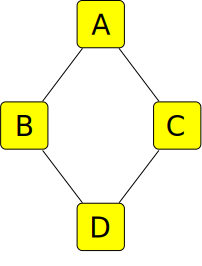
\includegraphics[width=.3\textwidth]{desarrollo/diseno/grafos_yaml_original}}\quad
    \subfigure[�rbol sin enlaces]{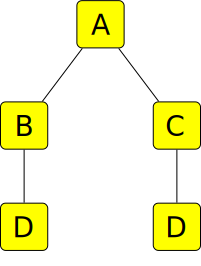
\includegraphics[width=.3\textwidth]{desarrollo/diseno/grafos_yaml_arbolsinenlaces}}\quad
    \subfigure[�rbol con enlaces]{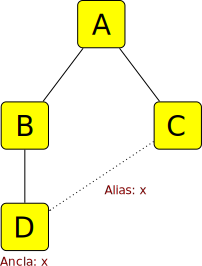
\includegraphics[width=.3\textwidth]{desarrollo/diseno/grafos_yaml_arbolconenlaces}}\quad
  }
  \caption{Representaci�n de grafos mediante �rboles XML}
  \label{fig:grafos_mediante_arboles}
\end{figure}

\subsubsection{Pruebas de unidad autom�ticas basadas en equivalencia}
\label{sec:yaxml_equivalencia}

\index{or�culo}

Un problema fundamental en la realizaci�n de pruebas de software es la
elaboraci�n de los \emph{or�culos}~\cite{Baresi:Oracles} necesarios
para comprobar si el comportamiento del software es el
esperado. Existe una gran variedad de tipos, seg�n la naturaleza del
software bajo prueba.

En lo que respecta a \yaxml{}, necesitamos un or�culo que nos diga si
un documento \ac{YAML} ha sido convertido a \ac{XML} sin p�rdidas ni
cambios en su informaci�n a nivel sem�ntico. Lo ideal es que sea lo
m�s autom�tico posible: no es factible programar un caso de prueba
para cada entrada. No podemos hacer comparaciones directas del texto,
pues un documento \ac{YAML} puede ser escrito en muchos estilos
distintos, y los documentos \ac{XML} tambi�n disponen de ciertos
mecanismos para el manejo del espaciado, por ejemplo.

Una posibilidad es generar un analizador de los documentos \ac{XML}
obtenidos, que construyera representaciones del estilo de las de
\modulo{YAML::XS} y las comparara con los grafos originales. Hay una
forma de conseguir algo similar con un esfuerzo mucho menor: podemos
aprovechar el hecho de que combinando \ac{YAXML} y \yaxml{} cerramos
el ciclo en torno a \ac{YAML} y \ac{XML}: podemos as� hacer una
transformaci�n \ac{YAML} $\rightarrow$ \ac{XML} $\rightarrow$
\ac{YAML}, y comparar los grafos resultantes de procesar los
documentos \ac{YAML} original y final. Si son equivalentes, dado que
\ac{YAXML} opera �nicamente sobre el documento \ac{XML}, sabremos que
�ste contiene toda la informaci�n del \ac{YAML} original sin
cambios. Se puede ver un esquema del proceso completo en la
figura~\ref{fig:oraculo_yaxml} de la p�gina~\pageref{fig:oraculo_yaxml}.

El principal inconveniente de este enfoque es que \ac{YAXML} tambi�n
introduce sus propios fallos, y �stos son vistos como fallos de
\yaxml{} por el conjunto de pruebas. Esto no tiene por qu� ser malo:
de hecho, puede verse como una forma de depurar los dos programas al
mismo tiempo, usando \yaxml{} como parte del or�culo de \ac{YAXML} y
viceversa.

Tiene la ventaja de ser completamente autom�tico: a�adir un nuevo caso
de prueba es simplemente a�adir un fichero \fichero{.yaml} bajo el
directorio \fichero{t/testInputs}.

\begin{figure}
  \centering
  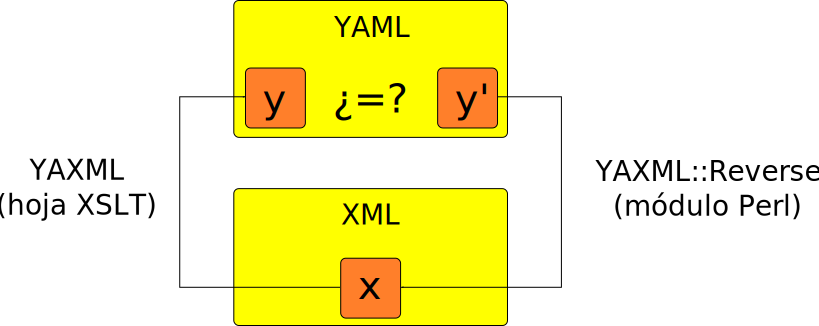
\includegraphics[width=.7\textwidth]{desarrollo/diseno/oraculo_yaxml}
  \caption{Or�culo de pruebas para \nombreyaxml{}}
  \label{fig:oraculo_yaxml}
\end{figure}

\subsubsection{Limitaciones de Perl frente a \acs{YAML}}
\label{sec:limitaciones}

\ac{YAML} se caracteriza por ser una especificaci�n muy flexible,
pudiendo combinar los tipos b�sicos de nodos y etiquetas de muchas
formas. Este fragmento de la especificaci�n~\cite{YAML}, que describe
a los nodos de vector asociativo, es particularmente interesante:

\begin{quotation}
  The content of a mapping node is an unordered set of key: value node
  pairs, with the restriction that each of the keys is unique. YAML
  places no further restrictions on the nodes. In particular, keys may
  be arbitrary nodes, the same node may be used as the value of
  several key: value pairs, and a mapping could even contain itself as
  a key or a value (directly or indirectly).
\end{quotation}

Como vemos, podemos tener claves no escalares e incluso referencias
c�clicas de un mapa como clave de uno de sus elementos. El problema de
los ciclos ya ha sido superado gracias a las anclas y alias, pero usar
claves no escalares es m�s dif�cil de resolver: los vectores
asociativos de Perl, usados como estructura de datos nativa por
\modulo{YAML::XS}, no admiten claves no escalares.

Existen m�dulos como \modulo{Tie::RefHash} que permiten usar clases
que implementan vectores asociativos con claves escalares y no
escalares como si fueran vectores asociativos normales, pero no los
reemplaza directamente, sino que modifica la forma en que Perl eval�a
el c�digo que usa el identificador de la variable ``sobrecargada''. Es
una t�cnica de bajo nivel: no podemos pasar ese vector asociativo y
usarlo en una subrutina como de costumbre, por ejemplo. Adem�s, y lo
que es m�s grave, no nos sirve una vez \modulo{YAML::XS} ha terminado
su procesado: tendr�a que usarse antes de asignarle cualquier
elemento.

Si us�ramos los diccionarios de Python, por ejemplo, uno podr�a
imaginarse emular claves basadas en nodos secuencia mediante tuplas, y
claves basadas en nodos de vector asociativo usando tuplas de
tuplas. Python no permite usar listas ni diccionarios como claves. Sin
embargo, al igual que en el caso de Perl, todo depender�a del
\emph{binding} que estuvi�ramos usando en ese momento.

De todas formas, examinando los lenguajes basados en \ac{YAML}
disponibles actualmente, no parece ser una restricci�n importante: a�n
no he podido encontrar un solo formato basado en \ac{YAML} que tenga
claves no escalares. \ac{JSON} sencillamente no tiene este problema.

Por ello, por lo pronto esta restricci�n se considera de baja
prioridad: solventarla requerir�a la reescritura completa de \yaxml{}
bajo otro entorno (seguramente una aplicaci�n escrita en C, \CPP o
Python), y no supondr�a realmente una ventaja para su uso general.

%%% Local Variables: 
%%% mode: latex
%%% TeX-master: "../../memoria"
%%% End: 

 
\subsection{Capa de aplicaci�n}
\label{sec:capa_aplicacion}
%%
%% Dise�o de la capa de aplicaci�n
%% Copyright (C) 2008 Antonio Garc�a Dom�nguez
%% $Id: capa_aplicacion.tex 622 2008-07-02 09:46:47Z antonio $
%%

La capa de aplicaci�n se ocupa de implementar las clases del modelo de
la arquitectura \ac{MVP}, y de proveer servicios de alto nivel
independientes de la interfaz gr�fica. Esto permite tener separados
todos los aspectos de la interfaz gr�fica respecto de aquellos
relacionados con la l�gica b�sica de \visor{}.

Veremos a continuaci�n cu�les son esas clases del modelo y servicios
ofrecidos, y qu� dise�o siguen.

%% Cambio de un enfoque basado en patrones a un enfoque en
%% componentes: no es cuesti�n de decir "mira, usamos patrones", sino
%% "este componente, por estas razones, ha requerido este patr�n, con
%% estos ajustes"

\subsubsection{Modelos de documentos}

% ModeloDocumento (comparar con ModeloPresentaci�nDocumento)

El concepto fundamental en \visor{} es el de un \clase{Documento}
\ac{XML} abierto por el usuario y preprocesado. Esta clase se ocupa de
encapsular toda esa informaci�n y gestionar los cambios en la hoja de
preprocesado utilizada y la realizaci�n de b�squedas.

N�tese que no se ocupa de la hoja de visualizaci�n: como detalle de
presentaci�n de que se trata, este aspecto se gestiona en su modelo de
presentaci�n, que veremos en \S\ref{sec:capa_presentacion_docs}
(p�gina~\pageref{sec:capa_presentacion_docs}).

Este modelo de documento integra los predicados de b�squedas mediante
palabra completa e ignorando min�sculas definidos mediante extensiones
XPath, dejando a las capas superiores �nicamente la responsabilidad de
definir las \clase{PeticionBusqueda} necesarias.

El conjunto de todas las clases empleadas, tanto del J2SE como de
\visor{}, se halla en el cuadro~\ref{fig:apl_docs}
(p�gina~\pageref{fig:apl_docs}).

\begin{figure}
  \centering
  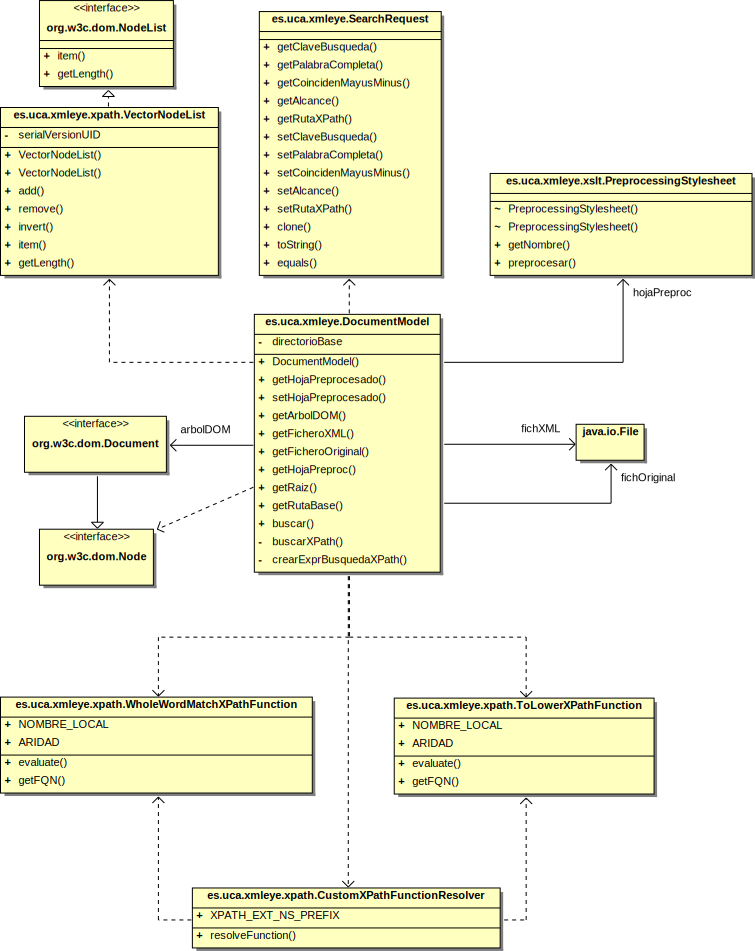
\includegraphics[width=\textwidth]{desarrollo/diseno/clases_xmleye_apl_documentos}
  \caption{Diagrama de clases de dise�o para modelado de documentos}
  \label{fig:apl_docs}
\end{figure}

\subsubsection{Hojas de estilos}

Las hojas de estilos participan tanto en la capa de presentaci�n como
en la capa de aplicaci�n. En la capa de aplicaci�n se halla toda la
infraestructura necesaria para su ejecuci�n, atendiendo a su
estructuraci�n en repositorios y soporte para localizaci�n, en
combinaci�n con el uso de herencia entre distintas hojas. Las propias
hojas son parte de la capa de presentaci�n.

Distinguiremos entre:

\begin{description}
\item[Hoja de usuario] 
  \index{hoja de usuario!definici�n}
  \index{hoja de usuario!punto de acceso}
  \index{hoja de usuario!preprocesado}
  \index{hoja de usuario!visualizaci�n}

  Conjunto cohesivo de una o m�s hojas \ac{XSLT} individuales
  seleccionable por el usuario que conforma un modo de preprocesar el
  documento o visualizar un nodo.

  Se distinguen dos tipos:
  \begin{description}
  \item[Preprocesado]
    Contienen transformaciones que afectan al documento \ac{XML}
    completo tras su apertura. Se usan para modificar el �rbol del
    documento o para realizar operaciones costosas como el
    establecimiento de enlaces.

  \item[Visualizaci�n] Contienen transformaciones a ejecutar sobre el
    nodo \ac{DOM} seleccionado por el usuario en cada momento.
  \end{description}

  Toda hoja de usuario contiene una o varias hojas \ac{XSLT}
  especiales cuyo nombre de fichero sigue el patr�n \fichero{(nombre
    hoja)[idioma[\_pa�s]].xsl}, donde [] indica una parte opcional y
  () una parte obligatoria. Llamamos a dichas hojas sus \emph{puntos
    de acceso}. Se intentar� antes acceder a los puntos de acceso m�s
  espec�ficos respecto del pa�s e idioma de la localizaci�n actual.

\item[Hoja \ac{XSLT}] Fichero individual que contiene un documento
  \ac{XML} definido sobre el vocabulario \ac{W3C} \ac{XSLT}.

\end{description}

Las hojas de usuario han de organizarse cumpliendo una serie de
requisitos:

\begin{itemize}
\item Han de poder ser f�cilmente localizables seg�n el pa�s y el
  idioma de la localizaci�n establecida por el usuario por defecto en
  su sistema.

\item Han de ser f�ciles de instalar, sin requerir configuraci�n
  alguna.

\item Han de ser f�ciles de elaborar, pudiendo basarnos en hojas de
  usuario ya existentes.
\end{itemize}

Los detalles de implementaci�n de cada tipo de hoja de usuario y
aquellos comunes a toda hoja de usuario han sido encapsulados en
clases, permitiendo a la capa de presentaci�n realizar
transformaciones sin conocer los detalles de la biblioteca \ac{XSLT}
usada.

En cuanto a los requisitos sobre la organizaci�n de las hojas de
usuario, se ha mantenido la separaci�n de responsabilidades moviendo
estos requisitos a una clase que act�a de \emph{repositorio}, que se
ocupa de localizar las hojas de usuario y configurarlas para conseguir
al mismo tiempo la capacidad de reutilizar c�digo y localizar las
hojas. La carga del repositorio se realiza al iniciar \visor{}.

La organizaci�n general de las clases utilizadas se halla en la
figura~\ref{fig:apl_hojasusuario} de la p�gina~\pageref{fig:apl_hojasusuario}.

\paragraph{Organizaci�n del repositorio}

El esquema de almacenamiento del repositorio no es configurable,
siendo as� posiblemente menos flexible, pero muy sencillo de
utilizar. La organizaci�n de las hojas de usuario se explica mejor con
un ejemplo. Una posible distribuci�n de hojas \ac{XSLT} de una
hipot�tica hoja de usuario de visualizaci�n llamada \fichero{perso}
bajo el directorio base con la ruta relativa \fichero{xslt} ser�a:

\begin{itemize}
\item \fichero{xslt/view/perso/perso.xsl}: punto de acceso inicial
  para la localizaci�n por omisi�n.
\item \fichero{xslt/view/perso/perso\_en.xsl}: punto de acceso inicial
  para la localizaci�n inglesa, sin especificar el pa�s.
\item \fichero{xslt/view/perso/perso\_en\_GB.xsl}: punto de acceso
  inicial para la localizaci�n inglesa en el Reino Unido.
\item \fichero{xslt/view/perso/logica.xsl}: hoja complementaria que
  permite que los tres idiomas compartan la misma l�gica.
\end{itemize}

Si fuera una hoja de preprocesamiento, se usar�a \fichero{preproc} en
vez de \fichero{view}.

\paragraph{Extensibilidad}
\label{sec:cod_xsl_acceso}

Las hojas de usuario son importadas por la hoja principal no
modificable de su tipo, en la ra�z del repositorio, que define la
m�nima funcionalidad com�n: \fichero{view.xsl} para las hojas de
visualizaci�n y \fichero{preproc.xsl} para las de preprocesado.

Adem�s, una hoja de usuario puede importar a otras y as�
especializarlas. Es el caso de \fichero{ppACL2}, que importa a
\fichero{xml}.

Para abstraer a las hojas de la l�gica de internacionalizaci�n, una
hoja de usuario que desee importar a otra puede usar \ac{URI}
especiales como \texttt{view\_ppACL2}. 

Mediante esta \ac{URI}, se acceder� a la hoja de usuario de
visualizaci�n \fichero{ppACL2} a trav�s del punto de acceso que mejor
se ajuste a la localizaci�n actual del usuario.

\paragraph{Internacionalizaci�n}
\label{sec:cod_xsl_l10n}

El ejemplo de \fichero{perso} anterior ilustra el mecanismo de
localizaci�n establecido por la l�gica de la capa de aplicaci�n. Dicho
mecanismo imita al usado por los \clase{ResourceBundle}s de la
biblioteca est�ndar de Java.

Si la localizaci�n  actual por defecto es ``es\_ES'' (espa�ol, Espa�a) y se
busca la hoja de visualizaci�n \fichero{ppACL2},
\clase{ControlHojasXSL} intentar� localizar un punto de acceso en el
siguiente orden:
\begin{enumerate}
\item \fichero{xslt/view/ppACL2/ppACL2\_es\_ES.xsl}
\item \fichero{xslt/view/ppACL2/ppACL2\_es.xsl}
\item \fichero{xslt/view/ppACL2/ppACL2.xsl}
\end{enumerate}

\begin{figure}
  \centering
  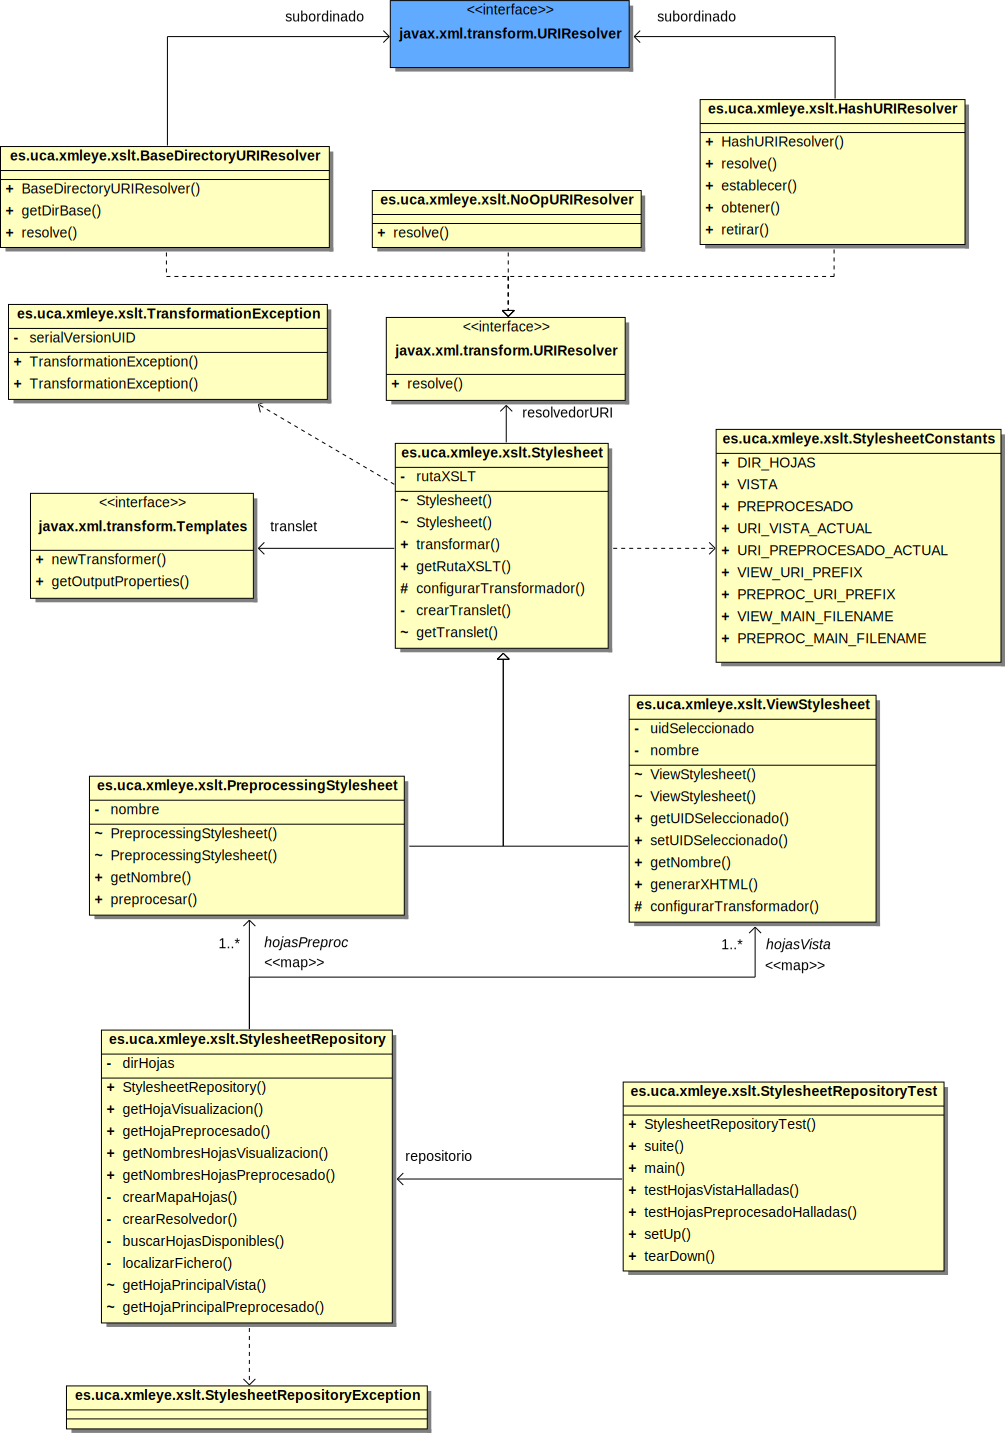
\includegraphics[width=.9\textwidth]{desarrollo/diseno/clases_xmleye_apl_hojas}
  \caption{Diagrama de clases de dise�o para las hojas de usuario}
  \label{fig:apl_hojasusuario}
\end{figure}

\subsubsection{Descriptores de formatos}

Otro servicio tambi�n a prestar por la capa de aplicaci�n es el de la
gesti�n de los descriptores de formatos de documento. Al igual que en
el caso de las hojas, se necesitaba abstraer a las capas superiores de
los detalles de un descriptor individual y de la forma en que se
hallan organizados.

Volvemos a tener otro repositorio, esta vez de descriptores, en el que
se siguen una serie de convenciones para evitar la necesidad de
realizar cualquier tipo de configuraci�n. A diferencia del repositorio
de hojas, no tratamos con un �nico �rbol de directorios: se pueden
encadenar varios, y as� poder tener una serie de ajustes a nivel
global para todos los usuarios, y otros locales para el usuario
actual. Para restaurar los ajustes locales a los globales, s�lo hemos
de borrar el descriptor a nivel local y actualizarlos.

\index{patr�n de dise�o!Observador}
\index{Singleton|see{patr�n de dise�o!Observador}}

Este repositorio abstrae tambi�n la l�gica que hace corresponder un
descriptor a un fichero determinado, y se ocupa de validar contra un
XML Schema todos los descriptores. El repositorio es un
\clase{AbstractListModel} de Swing, por lo que puede integrarse
f�cilmente como modelo de un formulario e incluso registrar
\patron{Observador}es sobre �l si se estima necesario, pero no es obligatorio.

Por otro lado, las clases para los descriptores individuales
encapsulan el formato de estos ficheros y proporcionan toda la
validaci�n necesaria de su contenido, lanzando excepciones cuando se
intentan establecer valores no v�lidos en alg�n atributo.

Las clases implicadas se hallan en el
cuadro~\ref{fig:aplicacion_formatos} de la
p�gina~\pageref{fig:aplicacion_formatos}.

\begin{figure}
  \centering
  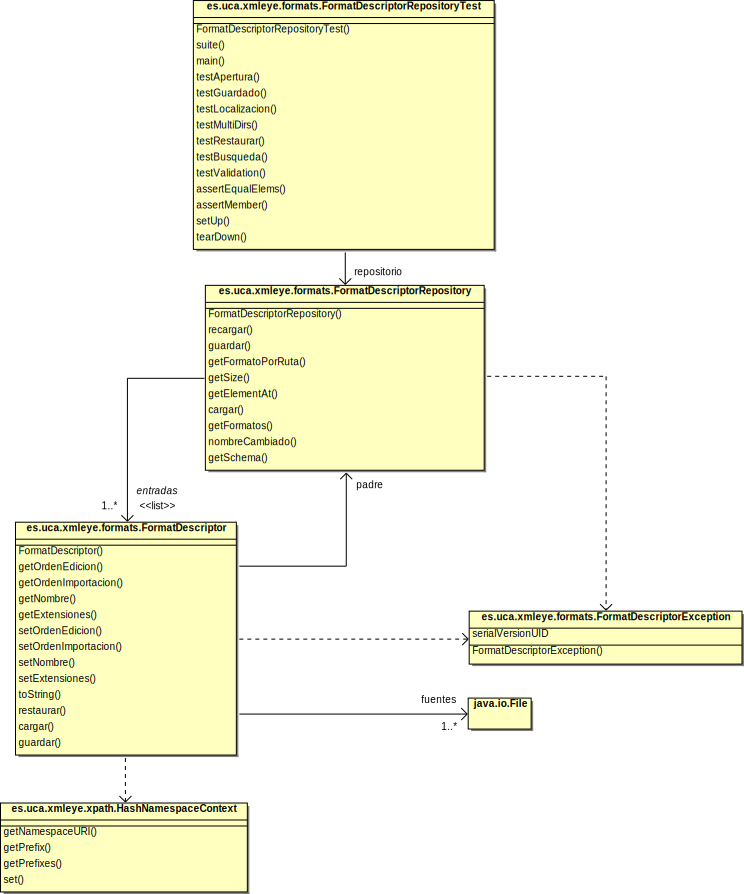
\includegraphics[width=\textwidth]{desarrollo/diseno/clases_xmleye_apl_descriptores}
  \caption{Diagrama de dise�o de clases de descriptores de formatos}
  \label{fig:aplicacion_formatos}
\end{figure}

% , descriptores de formatos (detalles
% de almacenamiento multinivel en repositorio, abstracci�n de los
% ficheros en forma de objetos, localizaci�n, restauraci�n)

\subsubsection{Notificaci�n de cambios sobre ficheros}

\index{patr�n de dise�o!Observador}
\index{Singleton|see{patr�n de dise�o!Observador}}

Un requisito muy interesante era el de poder vigilar los cambios
realizados sobre los documentos durante su visualizaci�n, pudiendo
mantener el editor y \visor{} abiertos en paralelo. Para ello se ha
implementado una clase que ofrece una interfaz basada en el patr�n
Observador, que se basa en la fecha de modificaci�n para notificar de
cambios en los contenidos del fichero.

Para ello, se usa un hilo en segundo plano de baja prioridad, que se
despierta cada cierto tiempo, realiza la comprobaci�n y vuelve a
dormir. Esto evita la p�rdida de rendimiento que supondr�a un bucle de
espera activa. Adem�s, las actualizaciones pueden pausarse y
reactivarse a voluntad.

% Observador

\subsubsection{Persistencia de preferencias}

% Singleton (�nicamente como punto de acceso, permite cambio backend en un futuro)

\label{sec:aplic_singleton}
\index{patr�n de dise�o!Inyecci�n de Dependencias}
\index{patr�n de dise�o!Singleton}
\index{Inyecci�n de Dependencias|see{patr�n de dise�o!Inyecci�n de Dependencias}}
\index{Singleton|see{patr�n de dise�o!Singleton}}

En este caso es fundamental tener un punto de acceso central a todas
las preferencias de los usuarios. Por estas razones, en la versi�n
original del visor se utiliz� el patr�n \patron{Singleton}, asegurando
la existencia de una �nica instancia de una clase que implementara una
interfaz. Se utiliz� una versi�n mejorada de la implementaci�n usual
tomada de~\cite{gof}, simplificando sobre la sugerida
en~\cite{singletonjava}.

Sin embargo, durante el desarrollo de esta nueva versi�n, se vio que
el uso del Singleton dificultar�a la posterior realizaci�n de pruebas
con sustitutos, e introduc�a una dependencia innecesaria. 

Para retirarla, se aplic� el patr�n \patron{Inyecci�n de
  Dependencias}: ahora no son las clases las que solicitan el gestor
de preferencias, sino las que lo reciben a trav�s de su
constructor. De esta forma, no se necesita el punto �nico de acceso
como antes, siendo muy f�cilmente sustituible durante pruebas, por
ejemplo, y manteniendo la independencia respecto a la implementaci�n a
trav�s del uso de una interfaz.

El diagrama de las clases involucradas en la gesti�n de preferencias
se halla en el cuadro~\ref{fig:dc_aplic_prefs} de la
p�gina~\pageref{fig:dc_aplic_prefs}. Podemos ver que el
\patron{Singleton} ha desaparecido, al ser ahora completamente
innecesario.

Se dispone de un valor booleano almacenado directamente en
dependencias, de tal forma que una clase que requiera un atributo con
persistencia entre las preferencias s�lo tendr� que instanciar
apropiadamente esta clase y luego utilizar \lstinline{get()} y
\lstinline{set()} sin m�s complicaciones.

%% sigue igual, pero cuidado con las fachadas

En el diagrama de secuencia~\ref{fig:ds_aplic_prefs} de la
p�gina~\pageref{fig:ds_aplic_prefs} puede verse c�mo se gestionan
las preferencias a lo largo del programa:
\begin{itemize}
\item Al iniciarse \visor{}, se crea una instancia de la clase
  principal que representa a toda la aplicaci�n. Esta clase es la
  ocupada de ensamblar a todas las dem�s clases de mayor nivel,
  inyectando las dependencias consideradas oportunas y evitando que
  dependan demasiado entre s�.

\item La clase principal ensambladora crea una instancia de la
  implementaci�n de gesti�n de preferencias a usar, y solicita que se
  carguen las preferencias.

\item La clase principal ensambla el modelo de presentaci�n de la
  ventana principal con el gestor de preferencias (visto a trav�s de
  su interfaz) y otros par�metros. Tambi�n ensambla y lanza la ventana
  principal.

\item Al cerrar la aplicaci�n, la misma clase principal solicita el
  guardado de las preferencias antes de terminar la ejecuci�n del
  programa.

\end{itemize}

\begin{figure}
  \centering
  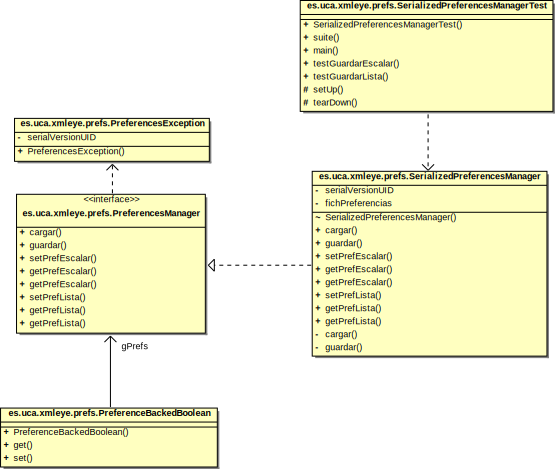
\includegraphics[width=\textwidth]{desarrollo/diseno/clases_xmleye_apl_prefs}
  \caption{Diagrama de clases de dise�o de gesti�n de preferencias}
  \label{fig:dc_aplic_prefs}
\end{figure}

\begin{figure}
  \centering
  \includegraphics[width=\textwidth]{desarrollo/diseno/diag_sec_xmleye_prefs}
  \caption{Diagrama de secuencia de gesti�n de preferencias}
  \label{fig:ds_aplic_prefs}
\end{figure}

%%% Local Variables: 
%%% mode: latex
%%% TeX-master: "../../memoria"
%%% End: 

 
\subsection{Capa de presentaci�n}
\label{sec:capa_presentacion}
%%
%% Dise�o de la capa de presentaci�n
%% Copyright (C) 2009 Antonio Garc�a Dom�nguez
%% $Id: capa_presentacion.tex 621 2008-07-02 09:04:44Z antonio $
%%

%% Organizaci�n general de la interfaz
%
% - cada documento tiene su modelo de presentaci�n, conectado al de la
% ventana principal.
%
% - ventana principal tiene su modelo de presentaci�n.
%
% - ventana de formatos tiene su modelo, usado por la ventana
% principal, pero sin conocimiento del modelo de presentaci�n de
% formatos
%
% - ventanas "acerca de" y "buscar" _no_ tienen modelos de
% presentaci�n, al ser muy simples. Ventana de Buscar se comunica con
% la principal a trav�s de un patr�n Observador, evitando que est�
% acoplada al modelo de presentaci�n completo. Ventana "Acerca de" es
% pr�cticamente un di�logo est�tico, por lo que no hay nada de
% interesante en su dise�o.
% 
% - vistas (DocumentView, DocumentList, WndMain, etc.) sincronizan por
% su cuenta con los modelos de presentaci�n, evitando complicar estos
% con los detalles de los controles GUI usados, y mejorando la
% capacidad para hacer pruebas respecto a la versi�n anterior.
%%

La capa de presentaci�n se encarga de la comunicaci�n persona-m�quina,
realizando peticiones sobre la capa de aplicaci�n y mostrando los
resultados.

Durante el dise�o de la interfaz, se usaron las
obras~\cite{jlfguid,jlfguidadv} como gu�a, como en el caso del dise�o
del di�logo ``Buscar'', donde el reparto de los componentes sigue sus
recomendaciones. Otras recomendaciones seguidas son la ejecuci�n de
las tareas largas en segundo plano, los elementos de los que deben
constar los men�s, o las combinaciones de teclas recomendadas para
cada opci�n.

\subsubsection{Estructura general}
\label{sec:capa_presentacion_general}

\index{patr�n arquitect�nico!MVP}
\index{patr�n arquitect�nico!Modelo de Presentaci�n}

Como ya se coment� en \S~\ref{sec:arquitectura_mvp}
(p�gina~\pageref{sec:arquitectura_mvp}), la capa de presentaci�n se
ocupar�a de los elementos Vista y Presentaci�n del tr�o
Modelo-Vista-Presentaci�n. En particular, se utilizar�a la variante
\patron{Modelo de Presentaci�n}, que nos permite definir la l�gica de
una forma completamente separada de la interfaz, y as� poder crear
nuevas interfaces de manera mucho m�s libre.

\visor{} dispone b�sicamente de 4 formularios, tal y como se
estableci� durante el an�lisis (apartado~\ref{sec:req_externas} en la
p�gina~\pageref{sec:req_externas}): el formulario principal, el
formulario de gesti�n de descriptores de formatos, el formulario de
realizaci�n de b�squedas, y por �ltimo el formulario con informaci�n
acerca de \visor{}.

Descartando el �ltimo de este apartado por su sencillez, podemos ver
que el formulario principal y el de gesti�n de formatos son los m�s
complejos. Por ello, modelaremos su estado con \patron{Modelos de
  Presentaci�n}, permitiendo una mejor comprensi�n y depuraci�n de su
c�digo. El formulario de b�squeda es m�s sencillo, y por lo tanto no
requiere dicho enfoque, como veremos posteriormente.

Adem�s de los modelos de presentaci�n, hablaremos en el resto de esta
secci�n de otros aspectos interesantes del dise�o de la capa de
presentaci�n.

\subsubsection{Modelos de presentaci�n y su ensamblaje}
\label{sec:capa_presentacion_docs}

\index{patr�n de dise�o!Observador}
\index{patr�n de dise�o!MVP}
\index{patr�n de dise�o!Inyecci�n de Dependencias}

En los formularios m�s complejos, se pudo ver r�pidamente que el uso
del patr�n \patron{Observador} para aspectos como el control de hojas
usadas y dem�s hac�a el c�digo cada vez m�s dif�cil de estructurar y
depurar. Adem�s, este c�digo imped�a poder aislar de manera efectiva
el estado de m�ltiples documentos.

Por ello, se cambi� a un enfoque donde unas clases encapsulan el
estado de la interfaz, de forma independiente a los controles
Swing. Estas clases ofrecen una serie de m�todos \metodo{get} p�blicos
para acceder al estado de la interfaz, y disponen tambi�n de un m�todo
por cada gesto de inter�s que pueda provenir del usuario.

Las vistas se reducen, por lo tanto, a informar de los gestos del
usuario al modelo de presentaci�n y posteriormente sincronizarse con
los modelos. Al quedarse sin la mayor parte de su l�gica, el hecho de
no poder realizar pruebas sobre los propios controles Swing no es tan
importante: podemos hacer pruebas sobre el modelo de presentaci�n,
enviando los gestos y estudiando su estado posterior.

Los modelos de presentaci�n pueden anidarse: as�, el modelo de
presentaci�n del formulario principal contiene a los modelos de
presentaci�n de cada documento, que contienen a su vez a los modelos
(ya no de presentaci�n) de los documentos correspondiente, junto con
otros elementos como una referencia al repositorio de hojas o al
repositorio de descriptores de formato. Entre los campos de todo
modelo de presentaci�n se encuentra el nodo seleccionado actualmente,
la hoja de visualizaci�n que est� siendo usada o la �ltima b�squeda
realizada, por ejemplo.

Los modelos de presentaci�n dependen de otros objetos, como ya hemos
visto, pero no deber�an quedarse acoplados a una implementaci�n o
instancia particular de ellos. En su lugar, estas dependencias se
proporcionan a trav�s del constructor, constituyendo una
\patron{Inyecci�n de Dependencias}. Los modelos de presentaci�n y sus
dependencias y la vista del formulario principal son creados y
configurados por un ensamblador central: la clase principal de la
aplicaci�n. Esto asegura que toda la l�gica relevante se halle en un
�nico sitio, y el resto de las clases se mantengan lo m�s flexibles
posible.

El diagrama de clases que describe las relaciones entre las distintas
vistas principales (formularios, listas de pesta�as y pesta�as) y los
modelos de presentaci�n se halla en el
cuadro~\ref{fig:presentacion_modpre} de la
p�gina~\pageref{fig:presentacion_modpre}.

\begin{figure}
  \centering
  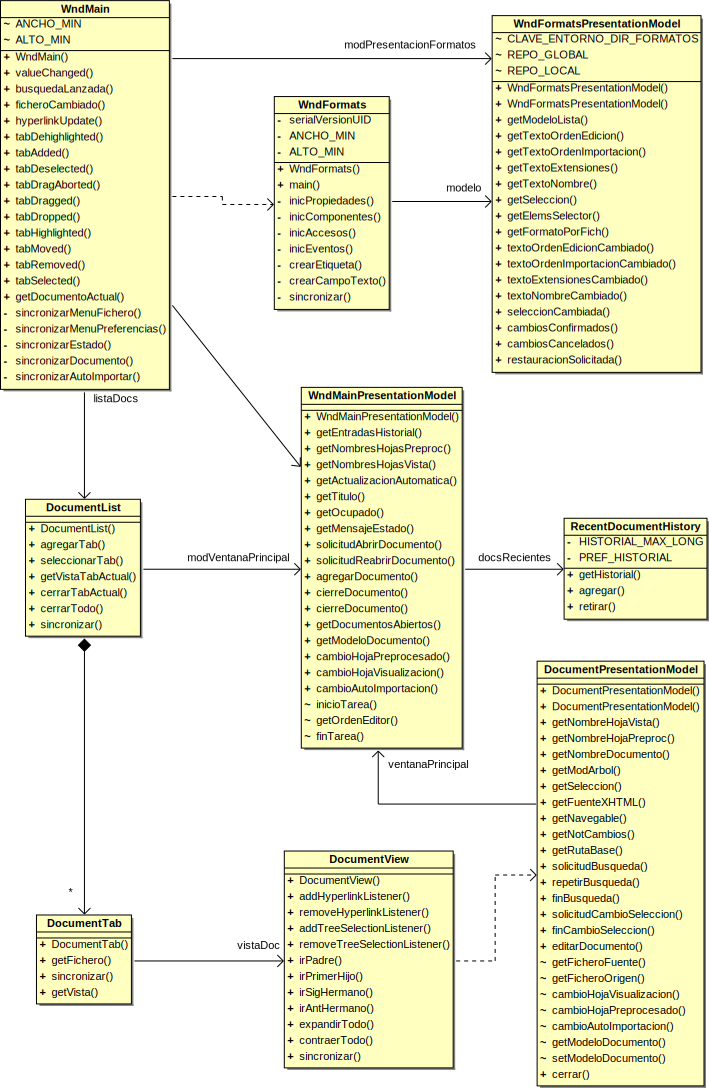
\includegraphics[width=.9\textwidth]{desarrollo/diseno/clases_xmleye_pre_modelos}
  \caption{Diagrama de clases de dise�o de los modelos de presentaci�n}
  \label{fig:presentacion_modpre}
\end{figure}

\subsubsection{Dise�o e integraci�n del formulario de b�squeda}

% Patr�n Observador

\index{patr�n arquitect�nico!Observador}

El formulario de b�squeda es una excepci�n al uso del patr�n
\ac{MVP}. Este di�logo carece pr�cticamente de l�gica propia, siendo
�nicamente una interfaz a partir de la cual el usuario puede construir
la petici�n de b�squeda y enviarla a sus suscriptores, entre los
cuales se halla el modelo de presentaci�n del formulario principal.

Aplicando de esta forma el patr�n \patron{Observador}, se evita el
acoplamiento del formulario de b�squeda al formulario principal, y se
puede guardar el evento para posteriormente repetir la b�squeda sin
necesidad de volver a mostrarlo, por ejemplo.

El formulario principal, como es com�n, se limita a notificar del
gesto al modelo de presentaci�n, que utiliza la funcionalidad del
modelo del documento para implementar la b�squeda, a�adiendo algo m�s
de inteligencia en lo que respecta a b�squedas repetidas.

Puede verse el diagrama de clases de dise�o correspondiente en el
cuadro~\ref{fig:presentacion_busq} de la p�gina~\pageref{fig:presentacion_busq}.

\begin{figure}
  \centering
  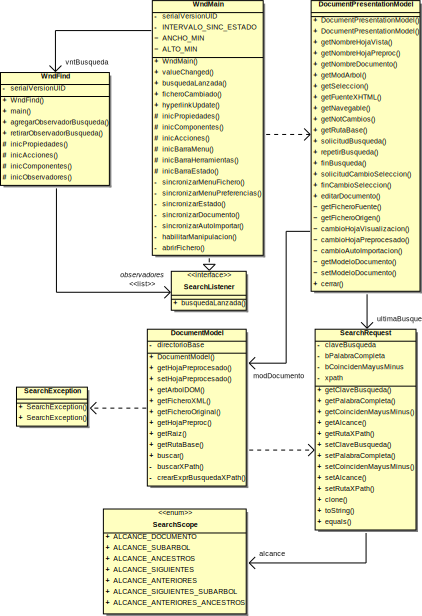
\includegraphics[width=.9\textwidth]{desarrollo/diseno/clases_xmleye_pre_busqueda}
  \caption{Diagrama de clases de dise�o de b�squedas}
  \label{fig:presentacion_busq}
\end{figure}

\subsubsection{Gesti�n de di�logos de mensajes}
\label{sec:presentacion_mensajes}

\index{patr�n arquitect�nico!Singleton}

%% SI: pero la necesidad viene de refactorizar en una clase com�n
%% informes de errores que vengan de otros hilos que no sean el de la
%% interfaz Swing, y de usar el patr�n Singleton para evitar tener que
%% usar m�todos est�ticos, que restar�an flexibilidad para el futuro.

A diferencia del caso de~\S\ref{sec:aplic_singleton}, se ha mantenido
el uso del patr�n \patron{Singleton} para la gesti�n de di�logos de
mensaje: el punto de acceso global en este caso es realmente
necesario, y la l�gica que provee es muy concreta.

En particular, la clase a la que da acceso el \patron{Singleton}
permite mostrar esos di�logos de forma independiente al hilo en que
nos hallemos: normalmente, para poder lanzar un di�logo debemos
hacerlo en el hilo de Swing, o se crear�n condiciones de carrera
indeseadas. Esta clase hace uso de las \clase{SwingUtilities} para
enviar las tareas apropiadas al hilo de Swing desde cualquier otro de
los hilos, como cuando estamos convirtiendo un documento de entrada,
por ejemplo.

Sin embargo, en este caso, no se ha dividido en una interfaz y una
implementaci�n, ya que a diferencia de la gesti�n de preferencias, no
se est�n considerando implementaciones alternativas.

\subsubsection{Presentaci�n de �rboles XML dirigidos por datos}
\label{sec:presentacion_mvc}

\index{patr�n arquitect�nico!MVC}
\index{patr�n arquitect�nico!Documento-Vista}

Los componentes usados para visualizar �rboles \ac{DOM} \ac{XML}
emplean, como todo componente Swing, una modificaci�n~\cite{swingarch}
del patr�n \patron{Modelo-Vista-Controlador} original de~\cite{gof}.

En esta versi�n modificada, llamada ``arquitectura de modelo
separable'' por Sun y similar al patr�n \patron{Documento-Vista} mencionado
en~\cite{archpatterns}, se dividen los componentes en tres partes:
\begin{itemize}
\item El componente Swing que implementa los aspectos de vista y
  controlador.
\item El objeto del Look \& Feel instalado en el componente Swing que
  define el aspecto exacto del componente.
\item El modelo del componente, es decir, la informaci�n que contiene,
  y que modifica su visualizaci�n o comportamiento. En Swing, el
  modelo puede contener tambi�n detalles de la interfaz gr�fica: bot�n
  activado o desactivado, por ejemplo.
\end{itemize}

As�, se han definido dos \clase{TreeModel}:
\begin{description}
\item[\clase{DOMTreeModel}] 

  Modelo sobre un �rbol \ac{DOM} \ac{XML} est�ndar, que hace
  accesibles los nodos de tipo elemento.

\item[\clase{DataDrivenTreeModel}] 

  Especializaci�n del anterior, este modelo incorpora la capacidad de
  realizar falsas podas, ocultando nodos de la visualizaci�n sin
  eliminarlos del �rbol \ac{DOM}.

  La decisi�n de ocultar un nodo o sus hijos se halla en el propio
  documento \ac{XML}. De esta forma, el usuario puede controlar este
  aspecto a trav�s de las hojas \ac{XSLT}, dirigi�ndolo todo por
  datos.

  En los campos \metodo{ATTRIBUTE\_LEAF} y \metodo{ATTRIBUTE\_HIDDEN} de
  \clase{DataDrivenTreeModel} se hallan los atributos que deben
  tomar el valor del campo \metodo{ENABLED\_VALUE} para activar la
  ocultaci�n de los hijos o del propio nodo, respectivamente.
\end{description}

Por las mismas razones que \clase{DataDrivenTreeModel}, se implement�
l�gica de dibujado dirigida por datos de los nodos del \clase{JTree}
mediante la clase \clase{DataDrivenTreeCellRenderer}. Este dibujador
puede modificar el icono y la etiqueta de un nodo a trav�s de sus
propios atributos \metodo{NODELABEL\_ATTRIBUTE} y
\metodo{NODEICON\_ATTRIBUTE}.

Se extendieron las capacidades de \clase{JTree} en \clase{DOMTree},
implementando operaciones para encapsular la navegaci�n por el �rbol y
abstraer al resto de la interfaz de los detalles, como
\metodo{selectParent}.

En la figura~\ref{fig:dc_presentacion_arboles}
(p�gina~\pageref{fig:dc_presentacion_arboles}) se ilustran en un
diagrama \ac{UML} las relaciones entre las clases relacionadas con la
visualizaci�n de �rboles \ac{XML}, incluyendo sus casos de prueba.

\begin{figure}
  \centering
  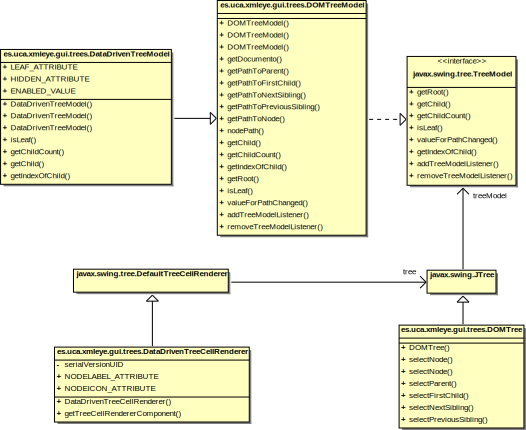
\includegraphics[width=\textwidth]{desarrollo/diseno/clases_xmleye_pre_arboles}
  \caption{Diagrama de clases de manejo de �rboles}
  \label{fig:dc_presentacion_arboles}
\end{figure}

\subsubsection{M�ltiples m�todos de acceso a una acci�n por el usuario}
\label{sec:presentacion_orden}

\index{patr�n arquitect�nico!Orden}

Otro patr�n de dise�o empleado com�nmente en las interfaces gr�ficas
es el patr�n Orden, y esta interfaz no es una excepci�n. 

En este patr�n, se define una interfaz para una acci�n gen�rica. El
lanzador de las acciones recibe objetos que cumplen tal interfaz. Al
generarse el evento de inter�s, reacciona ejecutando cada una de las
acciones a trav�s de dicha interfaz.

Este patr�n permite aislar al elemento que lanza la acci�n del que
realiza la acci�n. As�, podemos asociar cualquier acci�n a un control
Swing, sin que deba saber exactamente qu� hace esa acci�n. S�lo conoce
la interfaz que debe cumplir la acci�n, limit�ndose a invocar al
m�todo correspondiente.

Adem�s de reducir el acoplamiento, tambi�n mejora la estructura del
programa evitando la duplicaci�n de c�digo al codificar la misma
l�gica en varios componentes.

Es el caso usual de las acciones disponibles mediante la barra de
herramientas, un acceso de teclado y un elemento del men�, por
ejemplo: no importa exactamente qui�n lanza el evento, s�lo qu� acci�n
se lanza.

En Swing, la interfaz a cumplir es \clase{Action}, que permite no s�lo
unificar la orden a ejecutar, sino tambi�n parte de su visualizaci�n.
Podemos asignar un acelerador de teclado, una descripci�n corta y un
mnem�nico a una acci�n, y al crear un bot�n o elemento de men� a
partir de ella, �stos se inicializar�n con los valores correctos.


%%% Local Variables: 
%%% mode: latex
%%% TeX-master: "../../memoria"
%%% End: 


%%% Local Variables: 
%%% mode: latex
%%% TeX-master: "../../memoria"
%%% End: 


\section{Implementaci�n}
\label{sec:implementacion}
%%
%% Detalles de implementaci�n interesantes
%% Copyright (C) 2008 Antonio Garc�a Dom�nguez
%% $Id: implementacion.tex 629 2008-07-06 13:47:58Z antonio $
%%

\subsection{Perl}
\label{sec:codificacion_perl}

Se usaron la obra~\cite{perlbyexample} y la web~\cite{perldoc} como
referencias para los aspectos de divisi�n en m�dulos y la
implementaci�n en Perl del paradigma orientado a objetos.

Varios detalles de implementaci�n de ciertos patrones y otras
pr�cticas recomendadas para Perl se obtuvieron de~\cite{perloowiki}.

\lstset{language=Perl}

\subsubsection{Perl y el paradigma OO}
\label{sec:perl_oo}

No hay que confundir el hecho de emplear el paradigma orientado a
objetos con el uso de un lenguaje orientado a objetos.

Perl proporciona mecanismos para implementar la mayor�a de la
funcionalidad necesaria para este paradigma, pero no proporciona un
soporte directo a trav�s del lenguaje de muchas construcciones, como
una sintaxis espec�fica para declaraci�n de clases con palabras
reservadas para control de acceso, por ejemplo.

Otras veces ha de usarse una sintaxis algo m�s compleja de lo usual,
como en el caso de las variables de instancia.

Para implementar los m�todos, por ejemplo, Perl permite ``bendecir''
una referencia cualquiera con el nombre de un m�dulo. A partir de ese
momento, se buscar� la subrutina \metodo{metodo} dentro del m�dulo con
el que se bendijo \verb!$variable! al usar esta sintaxis:
\begin{lstlisting}
 $variable->metodo(@args);
\end{lstlisting}%$

Un m�dulo puede declarar a otros como base, que ser�n consultados
mediante un recorrido primero en profundidad sobre el �rbol de
generalizaciones durante la b�squeda de un m�todo. Este mecanismo es
el que implementa la herencia y los m�todos virtuales.

\subsubsection{Internacionalizaci�n}
\label{sec:cod_perl_l10n}

La internacionalizaci�n de los mensajes se consigue en
\postprocesador{} a trav�s del m�dulo \modulo{Locale::Maketext}, que
permite usar una jerarqu�a de clases donde la clase base define la
l�gica com�n y los idiomas por omisi�n y sus hijas contienen un
diccionario que realiza la localizaci�n para cada idioma (posiblemente
especificando el pa�s).

El uso es muy sencillo:
\begin{lstlisting}[caption=Ejemplo de uso de Locale::Maketext]
# Obtenemos el manejador a la localizaci�n que m�s se ajuste,
# subclase de ACL2::Localizacion, que es a su vez subclase
# de Locale::Maketext.
my $lh = ACL2::Localizacion->get_handle();

# Buscamos en el diccionario y sustituimos
# la cadena original: buscando 'Hola [_1]' se hallar�a 
# 'Hello [_1]' y luego se sustituir�a, dando 'Hello Pablo'.
print $lh->maketext("Hola [_1]", 'Pablo');
\end{lstlisting}

Dicho m�dulo es t�cnicamente superior al conocido \texttt{Gettext},
por la flexibilidad que su enfoque orientado a objetos le aporta: se
pueden definir funciones para manejar las formas plurales seg�n el
lenguaje, por ejemplo, simplemente redefiniendo un m�todo en la clase
correspondiente. 

Tambi�n numera los par�metros de las cadenas, permitiendo mayor
flexibilidad que la usual cadena con par�metros para \metodo{printf},
que da resultados pobres en casos en los que haya que cambiar el orden
de las palabras.

\subsubsection{Distribuci�n mediante \acs{PAR}}

Distribuir \postprocesador{} era bastante complejo e inc�modo en su
anterior versi�n. Se deseaba facilitar este aspecto en la mayor medida
de lo posible, permitiendo instalar de forma autom�tica las
dependencias o empaquetarlas en un formato c�modo de utilizar.

Este problema no es �nico a \postprocesador{}: empezando por \yaxml{},
pr�cticamente todo m�dulo sufre de �l. Existen muchas alternativas,
como \verb#perlcc# (retirado a partir de Perl 5.10), Perl2Exe o
Perl2App, pero entre todas ellas destacan \modulo{PAR} y
\modulo{PAR::Packer}.

De forma muy similar a los ficheros \fichero{.jar} de Java,
\modulo{PAR::Packer} y su herramienta \verb#pp# nos permiten crear
ficheros \fichero{.par} con todo el c�digo fuente de los conversores y
sus dependencias que no forman parte de los m�dulos est�ndar de
Perl. 

Instalar estos conversores y sus hojas se convierte en algo tan
sencillo como descargar el \fichero{.par} correspondiente a nuestra
plataforma y descomprimirlo sobre el directorio ra�z de
XMLEye. Adem�s, si nuestra aplicaci�n es Perl puro, el \fichero{.par}
generado puede ser usado en cualquier arquitectura y sistema
operativo.

Si no queremos obligar a nuestros usuarios a tener que instalar un
entorno Perl y los m�dulos \modulo{PAR} y \modulo{PAR::Packer} (cosa
particularmente molesta en Windows), tambi�n podemos crear ejecutables
monol�ticos, espec�ficos del sistema operativo y arquitectura bajo el
que se creen, que incluyen hasta el propio int�rprete de Perl con sus
m�dulos est�ndar.

Estas im�genes no son tan grandes como se esperar�a: los
\fichero{.par} para \yaxml{} y \postprocesador{} no llegan a los
100KiB, y los ejecutables, una vez comprimidos, no alcanzan los
2MiB. Adem�s, estas distribuciones comprimidas incluyen todos los
descriptores de formato y hojas de usuario necesarias.

\subsection{Java}
\label{sec:cod_java}

\lstset{language=Java}

Un texto �til ha sido la referencia del lenguaje~\cite{javalang},
escrita por los creadores de Java. La web~\cite{swingwiki} detalla
adem�s algunas pr�cticas recomendadas, funcionalidades no documentadas
y soluciones temporales a fallos conocidos de Swing.

Un ejemplo es la disponibilidad no documentada de fuentes con
anti-aliasing bajo la \ac{J2SE} 5.0, o la necesidad de forzar
manualmente un tama�o m�nimo sobre los hijos de \clase{JFrame}, un
fallo documentado en la propia base de datos de Sun y corregido en la
pr�xima \ac{J2SE} 6.0 ``Mustang''.

El uso del \ac{IDE} Eclipse 3.3.2 ha sido fundamental gracias a su
soporte para la realizaci�n sencilla de refactorizaciones a gran
escala, pudiendo renombrar m�todos y clases completas sin introducir
errores en el c�digo, entre otras cosas.

\subsubsection{Controles HTML}
\label{sec:cod_java_html}

Los controles para navegaci�n \ac{HTML} incluidos en Swing dejan
bastante que desear a la hora de usar el teclado para navegar o
seleccionar enlaces.

Para cubrir estas carencias, se especializ� la clase
\clase{JEditorPane} en \clase{Browser}.

Otros componentes �tiles incluyen un observador de enlaces capaz de
lanzar uno de los navegadores web del usuario (el navegador por
defecto en Windows y Mac OS X) al pulsar enlaces con \acs{URL}
v�lidas.

\subsubsection{Internacionalizaci�n}
\label{sec:cod_java_l10n}

En el lado de Java, la internacionalizaci�n se obtiene a partir de los
\clase{ResourceBundle}s, de los que hay dos tipos:
\begin{itemize}
\item \clase{PropertyResourceBundle}s, que acceden a ficheros
  \fichero{.properties} de f�cil mantenimiento, al s�lo contener
  cadenas de texto.
\item Especializaciones de \clase{ListResourceBundle}, que pueden
  contener cualquier tipo de objeto.
\end{itemize}

La capa de aplicaci�n s�lo maneja mensajes de texto y usa el primer
tipo, y la capa de presentaci�n usa el segundo tipo, al necesitar
adem�s iconos y atajos de teclado.

La clase \clase{ResourceBundle} de la biblioteca est�ndar de Java es
la ocupada de hallar e instanciar el \clase{PropertyResourceBundle} o
\clase{ListResourceBundle} que se ajuste mejor a la localizaci�n del usuario.

\paragraph{Componentes especializados}

Para facilitar la internacionalizaci�n, se han definido una serie de
clases gen�ricas que se inicializan a partir de un
\clase{ResourceBundle}.

En particular, se ha definido una especializaci�n de
\clase{AbstractAction} llamada \clase{ResourceBackedAction}, que
extrae sus valores de un \clase{ResourceBundle} que sigue un esquema
espec�fico de nombrado de claves.

La clase \clase{AbstractAction} es la clase base de todas nuestras
\patron{Orden}es (ver~\S\ref{sec:presentacion_orden}), que proporciona
implementaciones por defecto para la mayor�a de los m�todos de la
interfaz \clase{Action}, a seguir por toda \patron{Orden} de Swing.

Todas las �rdenes usadas son clases internas de
\clase{WndMain}: las m�s complejas tienen entidad propia, y
las dem�s son an�nimas. Puede verse un diagrama \ac{UML} de las
primeras en la figura~\ref{fig:diag_clases_impl_ordenes} de la
p�gina~\pageref{fig:diag_clases_impl_ordenes}.

\begin{figure}
  \centering
  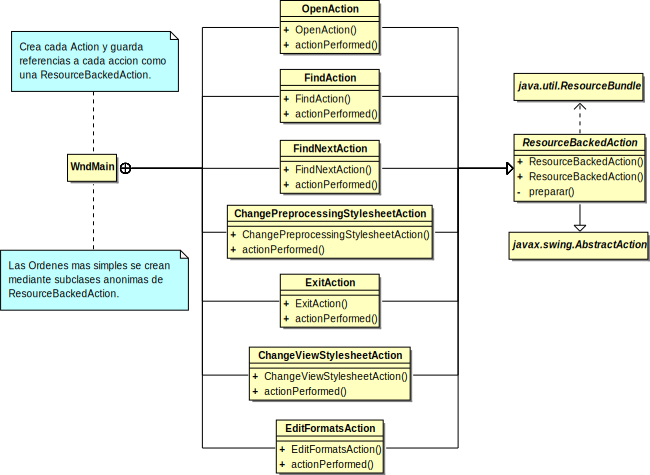
\includegraphics[width=.95\textwidth]{desarrollo/implementacion/clases_localizacion}
  \caption{Diagrama de clases de �rdenes}
  \label{fig:diag_clases_impl_ordenes}
\end{figure}

Tambi�n hay men�s (\clase{ResourceBackedMenu}) y botones
(\clase{ResourceBackedButton}) que extraen sus valores de los
\clase{ResourceBundle}.

\subsection{Hojas XSLT}
\label{sec:cod_xsl}

Las propias hojas \ac{XSLT} deben seguir una serie de convenciones en
su c�digo y forma de operar. Estas convenciones se hallan documentadas
en el apartado del manual de usuario dedicado a explicar c�mo crear
nuevas hojas \ac{XSLT}.

%%% Local Variables: 
%%% mode: latex
%%% TeX-master: "../../memoria"
%%% End: 


\section{Pruebas y validaci�n}
%%
%% Pruebas realizadas
%% Copyright (C) 2008 Antonio Garc�a Dom�nguez
%% $Id: pruebas.tex 635 2008-07-10 23:33:38Z antonio $
%%

Se dar� una breve introducci�n a los conceptos relacionados con las
pruebas de software en \ac{XP} y a continuaci�n se describir� el plan
de pruebas, junto con la especificaci�n de los casos de prueba y su
procedimiento de ejecuci�n.

\subsection{Pruebas en XP}
\label{sec:pruebas_xp}

La metodolog�a \ac{XP} realiza cuatro tipos de pruebas:

\begin{description}
\item[Pruebas de unidad] 
  \index{prueba!unidad} 

  Las pruebas de unidad comprueban de forma autom�tica la
  funcionalidad de un conjunto reducido y cohesivo de clases. Son
  escritas por los propios programadores, siguiendo la pr�ctica de
  \ac{XP} de la programaci�n basada en pruebas.

\item[Pruebas de aceptaci�n] 
  \index{prueba!aceptaci�n}

  Las pruebas de aceptaci�n son escritas
  por el propio cliente con asistencia de los miembros especializados
  en pruebas del equipo de desarrollo.

  M�s que probar el funcionamiento de un par de clases o de un m�todo
  determinado, lo que se intenta probar es la implementaci�n
  satisfactoria de una historia de usuario.

  As�, las pruebas de aceptaci�n suelen describirse mediante una serie
  de pasos en los cuales se utiliza el sistema completo para llevar a
  cabo una tarea. Cada paso tiene un resultado esperado asociado.

\item[Pruebas de integraci�n]
  \index{prueba!integraci�n}

  En \ac{XP}, las pruebas de integraci�n se realizan de forma
  constante. Aunque en mi caso no son importantes al ser un proyecto
  individual, \ac{XP} requiere que todo cambio hecho en una sesi�n de
  programaci�n (en parejas, por supuesto) sea integrado inmediatamente
  en el repositorio central.

  Por supuesto, esto implica que dichas modificaciones deben de haber
  pasado antes por todas las pruebas con �xito, asegur�ndonos de que
  no se han introducido nuevos fallos en otras partes del programa
  inadvertidamente.

\item[Pruebas de implantaci�n] 
  \index{prueba!implantaci�n}

  Una de las pr�cticas recomendadas (que no obligatorias) de \ac{XP}
  es la implantaci�n incremental. Desde el inicio de un proyecto, el
  sistema debe de implantarse en un entorno similar al real,
  posiblemente a menor escala, y comprobarse su correcto
  funcionamiento.

  Estas pruebas, sin embargo, no son especialmente importantes para
  una aplicaci�n de escritorio como la de este proyecto.

\end{description}

\subsection{Plan de pruebas}
\label{sec:pruebas_plan}

\subsubsection{Alcance}

Se determin� que, con las limitaciones de tiempo establecidas, no se
pod�an realizar pruebas de todas y cada una de las partes de \visor{},
\yaxml{} y \postprocesador{}.

Se decidi� implementar pruebas autom�ticas sobre los elementos
fundamentales y utilizar pruebas de aceptaci�n manuales sobre lo
dem�s. En particular, se descartaron aquellas clases cuya
funcionalidad depend�a en su mayor�a de bibliotecas externas, como la
interfaz gr�fica o el controlador de transformaciones \ac{XSLT}.

En un futuro, se espera reemplazar la mayor parte de las pruebas sobre
la interfaz por pruebas autom�ticas, utilizando los nuevos modelos de
presentaci�n. Actualmente ya se ha comenzado esta labor sobre el
di�logo de gesti�n de formatos.

\subsubsection{Tiempo y lugar}

Adem�s del propio uso frecuente de los conversores y \visor{}, mis
directores de proyecto contribuyeron a la ejecuci�n de pruebas de
aceptaci�n de manera informal a lo largo de la ejecuci�n del PFC.

Las pruebas se han realizado en todo momento durante el desarrollo del
PFC (especialmente las automatizadas), siguiendo la pr�ctica ``Flujo''
de \ac{XP}. Al final de cada iteraci�n, se dedic� un tiempo adicional
para la realizaci�n de pruebas de aceptaci�n manuales.

\subsubsection{Naturaleza de las pruebas}

La totalidad de las pruebas usadas son pruebas de caja negra, por ser
f�ciles de mantener a pesar de cambios en la implementaci�n.

\subsection{Dise�o de pruebas}
\label{sec:pruebas_diseno}

A primera vista, se puede determinar que existen cuatro elementos
fundamentales a probar:
\begin{itemize}
\item \postprocesador{}: �procesa correctamente la salida de
  \ac{ACL2}? �Se obtiene un documento que corresponda sin p�rdidas al
  original y que siga el formato de la \ac{DTD}? �Se trata de un
  m�dulo Perl correctamente estructurado y documentado?

\item \yaxml{}: �analiza sin errores los ficheros de entrada? �Realiza
  una conversi�n sin p�rdidas ni modificaciones de la informaci�n del
  fichero fuente \ac{YAML}? Al igual que en el caso anterior, �tiene
  un nivel m�nimo de calidad como m�dulo Perl?

\item El visor \visor{}: �se validan las entradas? �Se reacciona bien
  ante acciones no v�lidas del usuario? �Obtiene el usuario los
  resultados esperados?
\item La integraci�n entre los conversores y \visor{}: �se realiza con
  �xito? �Se capturan y muestran correctamente los fallos?
\end{itemize}

En base a esto, cada parte requiere una combinaci�n determinada de
varios tipos de pruebas:
\begin{description}
\item[\nombrepostprocesador{}] El desarrollo de este conversor se
  halla guiado por los enunciados Lisp y las salidas de \ac{ACL2} que
  ha de procesar. Por lo pronto, resulta natural estructurar las
  pruebas simplemente alrededor de dichos casos.

  Se puede implementar un mecanismo de pruebas de regresi�n usando
  estos enunciados: una vez se haya validado una salida determinada
  como correcta, se puede mantener dicha salida y comparar las salidas
  posteriores con ella, notificando cualquier cambio de inter�s de
  forma autom�tica.

  En un futuro, cuando el alcance del procesador se ampl�e a
  demostraciones de mayor envergadura, se a�adir�n pruebas de unidad
  sobre las clases de mayor importancia.

\item[\nombreyaxml{}] 

  De forma similar al caso anterior, el desarrollo y revisi�n de este
  conversor se apoya sobre una serie de entradas conocidas: cuando
  alguna entrada falla, se a�ade como caso de prueba y se revisa
  \yaxml{} hasta que vuelven a superarse todas las pruebas.

  A diferencia de \postprocesador{}, no necesitamos registrar las
  salidas anteriores ``buenas'' y compararlas con las actuales, sino
  que podemos usar el ciclo \ac{YAML} $\rightarrow$ \ac{XML}
  $\rightarrow$ \ac{YAML} implementado y establecer directamente la
  equivalencia sem�ntica de los dos ficheros \ac{YAML} original y
  final. Este proceso se halla descrito a mayor nivel de detalle
  en~\S\ref{sec:yaxml_equivalencia}
  (p�gina~\pageref{sec:yaxml_equivalencia}).

\item[\nombrevisor{}] 
  Se podr�a dividir \visor{} en tres partes:

  \begin{enumerate}
  \item La interfaz de usuario: Las limitaciones de tiempo, combinadas
    con la dificultad y la escasez en herramientas automatizadas de
    prueba de las interfaces gr�ficas obliga a usar pruebas de
    aceptaci�n manuales por lo pronto. En un futuro cercano, el nuevo
    dise�o de la capa de presentaci�n basado en modelos de
    presentaci�n permitir� automatizar estas pruebas, limit�ndonos a
    enviar notificaciones de gestos a los modelos de presentaci�n.

    Sin embargo, los componentes relacionados con los �rboles \ac{XML}
    son cruciales para la aplicaci�n, y deben de incluir sin falta
    pruebas automatizadas sobre las propiedades que deben cumplir y el
    comportamiento que deben seguir.

  \item Las hojas de usuario: aunque su realizaci�n ser�a t�cnicamente
    factible, las pruebas de unidad de estas hojas no podr�an
    mantenerse estables, puesto que el formato de salida no lo es: al
    ser \ac{XHTML}, est� sujeto a muchos cambios y retoques a lo largo
    del tiempo. Se puede decir lo mismo acerca del paso de
    preprocesado.

  \item La capa de aplicaci�n: esta capa provee los servicios b�sicos
    sobre los que se apoya la capa de presentaci�n. No probaremos
    aquellas partes que �nicamente dependan de la capa de servicios
    t�cnicos, como el funcionamiento de las transformaciones
    \ac{XSLT}, por ejemplo, pero s� los servicios de nivel superior.

    Por ejemplo, habr� que depurar los repositorios de hojas de estilo
    y de descriptores de formatos, la validaci�n de los campos de los
    descriptores de formato, la correspondencia entre rutas XPath y
    nodos de un �rbol \ac{DOM} \ac{XML}, o las extensiones XPath,
    entre otras cosas.
  \end{enumerate}

\item[Integraci�n] 

  La integraci�n es otro aspecto dif�cil de probar autom�ticamente,
  dado que depende en gran medida del entorno empleado por el usuario
  y de la configuraci�n que haya establecido.

  Sin embargo, se presta bien a pruebas de aceptaci�n manuales sobre
  una configuraci�n realizada de antemano. Se habr� de probar que la
  integraci�n reacciona bien a errores de los programas y de su
  invocaci�n, fallando cuando debe y permitiendo una recuperaci�n
  r�pida.

\end{description}

\subsection{Especificaci�n de los casos de prueba}
\label{sec:pruebas_especificacion}

\subsubsection{\nombrepostprocesador{}}
\label{sec:pruebas_postprocesador}

Cada una de las fuentes Lisp y su salida correspondiente a filtrar por
\postprocesador{} seg�n las historias de usuario planteadas es
utilizada como una prueba de regresi�n semiautom�tica.

Describiremos brevemente el contenido de las fuentes Lisp usadas como
casos de prueba. Por claridad, usaremos notaci�n infija. Todos estos
enunciados se encuentran bajo el subdirectorio \fichero{t/testInputs}
de \postprocesador{}.

Durante las pruebas se desactiva todo almacenamiento de resultados
intermedios y se obliga a actualizar el grafo completo de dependencias,
para evitar que en ejecuciones distintas de las pruebas se consigan
resultados distintos.

\begin{itemize}
\item \fichero{triple-rev}

  \fichero{triple-rev} fue el objetivo de la primera iteraci�n. En
  esta demostraci�n se comprueba para una funci�n de inversi�n de
  listas Lisp \evento{rev} que $$rev(rev(rev(x))) = rev(x)$$ para
  toda lista que le pasemos, sea cual sea su estructura.

\item \fichero{equal-app}

  En esta demostraci�n se comprueban ciertas propiedades acerca de las
  funciones \evento{app} para concatenaci�n de listas, \evento{dup}
  para duplicaci�n de cada elemento y \evento{properp} para
  comprobaci�n de listas propias, terminadas mediante \evento{nil},
  como \evento{(a b)} o \evento{(a . (b))} pero no \evento{(a . b)}.

  \begin{itemize}
  \item Asociatividad: $app(app(a,b), c) = app(a, app(b, c))$
  \item Distributividad de la duplicaci�n de cada elemento respecto de
    la concatenaci�n: $app(dup(a),dup(b)) = dup(app(a,b))$
  \item Toda lista a la que se a�ade \lisp{nil} es propia:
    $properp(app(a,nil))$.
  \end{itemize}

\item \fichero{fallo-defun}

  Realmente, este gui�n no trata de probar nada: est� dise�ado para
  ver si \postprocesador{} es capar de tratar los fallos en las
  demostraciones de los \orden{defun}.

  En primer lugar, declaramos una funci�n de c�lculo de factorial
  correcta, que siempre da un resultado correcto y siempre para.

  La siguiente versi�n err�neamente usa $=$ en vez de $zp$, y por lo
  tanto no para nunca para otra cosa que no sea un natural. $zp$ es
  verdadero para toda cosa que no sea un n�mero mayor que cero:
  listas, �tomos, enteros no positivos (incluyendo el cero, claro),
  etc. Sin embargo, $=$ s�lo es verdadero si lo que se pasa es cero,
  por lo que ante un n�mero negativo, por ejemplo, nunca llegar�a al
  caso base y se quedar�a siempre en el caso recursivo.

  En la tercera versi�n, no hay caso base: se ha reemplazado por una
  llamada recursiva a s� mismo. Y en la cuarta y �ltima, no se reduce
  el tama�o de la entrada, imposibilitando tambi�n la parada.

\item \fichero{hanoi}

  No es uno, sino realmente cuatro casos de prueba, al tratarse de un
  proyecto de \ac{ACL2} con tres ficheros Lisp. Tenemos un caso de
  prueba por fichero y otro caso de prueba m�s para la detecci�n del
  grafo que forman y su correcto uso:

  \begin{itemize}
  \item \fichero{hanoi-use.lisp} es el fichero ra�z del
    proyecto. Utiliza la orden \orden{include\hyp{}book} para acceder
    a la definici�n de la funci�n que resuelve el problema de las
    torres de Hanoi, \evento{hanoi::hanoi}, que se halla en el libro
    \libro{books/hanoi}.

  \item \fichero{books/hanoi.acl2} es el fichero Lisp que sirve para
    certificar los contenidos del libro \libro{hanoi} dentro de su mundo
    l�gico inicial. Se podr�a haber llamado \fichero{cert.acl2} si se
    hubiera deseado emplear para cualquier libro dentro de
    \fichero{books}, siguiendo las convenciones usuales de manejo de
    libros de \ac{ACL2}~\cite{ACL2:BookMakefiles}, pero se ha
    preferido esta forma espec�fica, para cuando se a�adan m�s libros
    posteriormente.

  \item \fichero{books/hanoi.lisp} es el propio libro con las
    definiciones necesarias, que asume que se halla dentro del mundo
    l�gico inicial definido por el fichero de certificaci�n
    anterior. Define las funciones \evento{move}, que genera una
    instrucci�n del tipo ``mover un disco de la pila A a la pila B'' y
    \evento{hanoi}, que resuelve el problema de las Torres de Hanoi
    para $n$ discos. Tambi�n incluye un teorema, \evento{len-append},
    que establece que la longitud de la concatenaci�n de dos listas es
    la suma de sus longitudes.

  \end{itemize}

\item \fichero{mapnil}

  En este caso, se demuestra la conmutatividad entre la duplicaci�n de
  los elementos mediante \evento{dup} y la sustituci�n de todo
  elemento de una lista Lisp por \evento{nil} mediante
  \evento{mapnil}.

\item \fichero{memp}

  Dada una funci�n \evento{memp} que comprueba la pertenencia de un
  elemento a una lista y otra funci�n \evento{app} que concatena dos
  listas, se demuestra que $$memp(e, app(a,b)) \equiv memp(e,a) \vee
  memp(e,b),$$ es decir, que todo elemento de la concatenaci�n de las
  dos listas pertenecer� a una u a otra.
  
\item \fichero{miscDefs}

  Comprobamos que \postprocesador{} es capaz de filtrar una
  diversidad de funciones, como b�squedas en diccionarios,
  implementaci�n de aritm�tica mediante el uso de la longitud de las
  listas, recolecci�n de elementos �nicos, potenciaci�n, etc.

  Algunos ejemplos:
  \begin{itemize}
  \item $mapnil(x)$ convierte todos los elementos a \lisp{nil}.
  \item $add(x,y)$ realiza la suma mediante el n�mero de elementos de
  ambas listas. Es decir, implementamos la suma creando una lista de 5
  elementos cuando nos dan una de 2 y otra de 3.
  \item $app(a,b)$ Concatenamos dos listas.
  \item $mem(e,x)$ Devuelve el primer par de la lista tal que el primer
    elemento sea $e$, o $nil$.
  \item $lonesomep(e,lst)$ Comprobamos que $e$ es �nico en la lista.
  \item $collect-lonesomep(a,b)$ Recoge los elementos de la lista $a$ que
    son �nicos en la lista $b$.
  \item $mult(x,y)$ Multiplica a trav�s de longitudes de listas. Si le damos
    una lista con 2 elementos y otra con 3, nos crea una lista con 6.
  \item $fact(n,a)$ Calcula el productorio en aritm�tica sobre
    longitud de listas de las sublistas de la lista que le pasemos.
  \item $fact1(n,a)$ Versi�n recursiva final de \evento{fact}.
  \item $foundp(x,a)$ Busca una clave dentro de un diccionario Lisp. Si el
    diccionario es la lista Lisp de la forma \lisp{((a 2) (b 3))}, sus
    claves son $a$ y $b$.
  \end{itemize}
  
\item \fichero{suma}

  Este caso comprueba que se tratan de forma correcta los
  \evento{defthm} que no requieren inducci�n alguna. Aqu�, \ac{ACL2}
  s�lo tiene que aplicar sus reglas predefinidas sobre la aritm�tica
  decimal para ver que $2 + 2 = 4$ o que $a + b + c = b + c + a$.

  Tambi�n se comprueba que se manejan bien los elementos de listas
  Lisp con la sintaxis \verb!|texto|!.

\item \fichero{swaptree}

  Se define una funci�n \evento{swaptree} que invierte dos �rboles
  Lisp, y se demuestra que es idempotente.

\item \fichero{tail-rev}

  Se define una implementaci�n trivial de la inversi�n de una lista
  \evento{rev} sabiendo que es correcta. Hecho eso, definimos una
  implementaci�n recursiva final obtenida por la transformaci�n
  mediante desplegado-plegado \evento{rev1}. Ahora comprobamos que
  est� bien hecha, es decir, que da los mismos resultados que la
  versi�n original.

\item \fichero{treecopy}

  Es parecida a \evento{swaptree}, pero en este caso lo que se hace es
  copiar un �rbol Lisp, y comprobar que dicha funci�n repite siempre
  la entrada que se le suministra.

\item \fichero{triple-rev-misspell}

  Este caso de prueba es una modificaci�n de \fichero{triple-rev} con
  un fallo en el nombre de un par�metro formal introducido
  intencionadamente, que origina una demostraci�n fallida de la
  longitud suficiente como para ser de inter�s. Adem�s, permite
  comprobar que se tratan bien los errores de \evento{defthm}.

\item \fichero{tutorialWebACL2}

  Este otro caso de prueba es el proyecto de un solo fichero m�s
  completo de todos. En este caso, se desea probar que un algoritmo
  para la inversi�n de una lista Lisp que s�lo hace uso de las
  funciones predefinidas \lisp{endp} (predicado para detectar el
  final de una lista), \lisp{cons} (creaci�n de un par Lisp),
  \lisp{car} (extracci�n de la cabecera) y \lisp{cdr} (extracci�n
  de la cola) es equivalente al algoritmo trivial.

  El proceso es algo m�s complicado que los ejemplos anteriores, y
  puede verse en~\cite{jsmweb}, donde se usa ``El M�todo'',
  acumul�ndose teoremas a demostrar en forma de una pila, donde un
  teorema puede requerir para su demostraci�n verificar otros teoremas
  o lemas.

  Se hacen uso de algunos elementos m�s avanzados, como \orden{thm},
  que lanza una demostraci�n pero no guarda sus resultados en el mundo
  l�gico de \ac{ACL2}, \orden{local} que evita que las reglas
  generadas por un evento sean accesibles fuera de un
  \orden{encapsulate} o libro, y \orden{encapsulate}, que permite
  realizar demostraciones controlando qu� reglas se producen y cu�l es
  la signatura de las funciones definidas.

\end{itemize}

Las pruebas de regresi�n comparan los �rboles \ac{XML} de los
resultados esperados con los obtenidos, empleando el m�dulo
\modulo{XML::SemanticDiff}. Las diferencias detectadas son filtradas
por un predicado que determinan si constituyen una regresi�n o
no. Actualmente, algunas de las diferencias ignoradas son:

\begin{itemize}
\item Cambios en los tiempos de ejecuci�n.
\item Cambios en la versi�n de \ac{ACL2}.
\item Cambios de may�sculas y min�sculas y barras en nombres de
  fichero en Windows.
\item Mensajes de compilaci�n durante la certificaci�n de un libro
  (dependen del compilador y sistema operativo usado).
\end{itemize}

Las pruebas de regresi�n no son las �nicas realizadas. Integradas
dentro del marco de pruebas creado por el m�dulo
\modulo{ExtUtils::MakeMaker} se hallan tambi�n algunas pruebas de
car�cter m�s general:

\begin{itemize}
\item El m�dulo principal debe de poder cargarse con �xito. Esto nos
  asegura de que no nos hayamos olvidado de instalar o referenciar a
  alg�n m�dulo importante en nuestro c�digo.

\item Se debe de haber retirado el texto in�til de las plantillas
  inicialmente generadas por \verb#h2xs#, la herramienta ocupada de
  crear el esqueleto b�sico de todo m�dulo Perl.

\item Todos los ficheros fuente del m�dulo Perl han de incluir el
  aviso de la licencia \ac{GPL}.
\end{itemize}

\subsubsection{\nombreyaxml{}}
\label{sec:pruebas_yaxml}

Como otro m�dulo Perl m�s, \yaxml{} emplea el mismo marco de pruebas y
las pruebas de car�cter general de \postprocesador{}. Este m�dulo usa
tambi�n pruebas de regresi�n, pero son completamente autom�ticas en
este caso, como ya se explic� anteriormente. Ciertas pruebas de
regresi�n son m�s bien para la versi�n refinada de \ac{YAXML}
implementada para cerrar el ciclo \ac{YAML} $\rightarrow$ \ac{XML}
$\rightarrow$ \ac{YAML} que para \yaxml{} en s�.

Algunos casos de prueba se corresponden con documentos reales usados
por herramientas conocidas, y algunos s�lo depuran ciertos aspectos
esenciales. Existe cierto solapamiento entre ambos tipos. Los ficheros
\fichero{.yaml} utilizados como casos de prueba son:

\begin{itemize}
\item \fichero{djangoJSON}

  Este es un ejemplo de un volcado de una base de datos realizado por
  el entorno de desarrollo de aplicaciones Web Django
  (\url{http://www.djangoproject.com/}). Tiene la particularidad de
  usar \ac{JSON}, un subconjunto de \ac{YAML} 1.1, motivando el cambio
  del m�dulo \modulo{YAML::Syck} a \modulo{YAML::XS}.

  % JSON: YAML 1.1

\item \fichero{djangoJSON\_blockIndicatorTest}

  % Indicador de texto

  Otro volcado de Django en el cual se hace patente la necesidad en
  \ac{YAXML} de tener cuidado con el espaciado en blanco y no
  cambiarlo inadvertidamente. En particular, hay que tener cuidado con
  el �ltimo salto de l�nea final, evitando introducirlo cuando
  originalmente no estaba, utilizando el indicador ``|-'' en el estilo
  de bloque para escalares.

\item \fichero{firefoxBookmarks}

  % Ejemplo del "mundo real", JSON, UTF-8

  Una copia de seguridad de los marcadores de Firefox 3 realizada
  tambi�n en \ac{JSON}, que en este caso ten�a la complicaci�n de
  emplear caracteres de \ac{UTF}-8, en particular ideogramas
  japoneses. Se identificaron y resolvieron diversas cuestiones
  relacionadas gracias a este ejemplo.

\item \fichero{fiveMinutes1}

  % Soporte b�sico

  Es uno de los casos m�s b�sicos: un flujo de 4 documentos que
  emplean secuencias de \ac{YAML}. Es compatible con \ac{YAML} 1.0 en
  adelante, al igual que todos los casos de prueba que vienen a
  continuaci�n.

\item \fichero{fiveMinutes2}

  % Claves que no son valores v�lidos en XML

  Este ejemplo muestra ejemplos de vectores asociativos de \ac{YAML}
  1.0, y fue el primer caso de prueba que mostraba la necesidad de
  rodear las limitaciones de \ac{XML} respecto a los identificadores
  v�lidos para una etiqueta utilizando los elementos \verb#_key# y
  \verb#_value#.

\item \fichero{fiveMinutes3}

  % Claves que requieren cuidado especial al devolverlas a YAML

  Desarrollando sobre el ejemplo anterior, este caso de prueba tambi�n
  usa claves de vectores asociativos no directamente representables en
  \ac{XML}, pero adem�s una de ellas requiere un especial cuidado a
  devolverla a \ac{YAML}, o producir�a un error de sintaxis, al
  contener la secuencia ``: ''.

\item \fichero{fiveMinutes4}

  % Estilos de bloques escalares

  Este caso de prueba utiliza los estilos literal y de l�neas reunidas
  para los escalares. En el estilo literal el espaciado no es
  modificado excepto por el indentado de cada l�nea. En el estilo de
  l�neas reunidas, todas las palabras separadas por �nicamente un
  car�cter de espaciado (como un espacio o un salto de l�nea) son
  reunidas en una sola l�nea.

\item \fichero{fiveMinutes5}

  % Estilos de bloque y flujo de colecciones

  El �ltimo ejemplo de la serie~\cite{YamlInFiveMinutes} ilustra c�mo
  pueden escribirse tambi�n las colecciones con distintos estilos, ya
  sea de bloque, con un elemento por l�nea, o de flujo, que permite
  definir m�s de un elemento en cada l�nea.

\item \fichero{invoice}

  % Manejo de anclas y alias (mapa anclado)
  % YAML complejo

  Este caso de prueba es uno de los ejemplos incluidos en la
  especificaci�n \ac{YAML}~\cite{YAML}, y precisamente el que ilustra
  el uso de anclas y alias para evitar tener que repetir el contenido
  com�n a dos nodos.

\item \fichero{mappingAnchoredSequence}

  % Manejo de anclas y alias (secuencia anclada)

  Aqu� probamos a transformar un documento en que el documento anclado
  no es un mapa, sino una secuencia.

\item \fichero{podExample}

  % Depura el ejemplo del POD de YAXML::Reverse

  Este ejemplo tan sencillo es el usado en la documentaci�n \ac{POD}
  de \yaxml{}, para poder garantizar que funcione.

\item \fichero{yaxmlReverseMETA}

  % YAML del "mundo real"
  
  Se trata del fichero \fichero{META.yaml} de \yaxml{}. Estos ficheros
  son utilizado por diversas herramientas autom�ticas, como las que
  utiliza el CPAN, para obtener informaci�n de autor�a y dependencias.

\end{itemize}

\subsubsection{Visor e integraci�n}
\label{sec:pruebas_visor}

\paragraph{Pruebas de unidad}
\label{sec:pruebas_visor_unidad}

Las pruebas de unidad definidas para cada clase comprueban una serie
de propiedades acerca de su comportamiento. En lugar de dar una
especificaci�n exacta de cada prueba (que s�lo ser�a repetir el
c�digo), listaremos las propiedades que verifican.

Estas pruebas, basadas en el marco JUnit, se ejecutan de forma
autom�tica y son un objetivo m�s dentro del fichero de tareas Ant.

Toda clase de pruebas tiene el nombre formado por el nombre de la
clase cuyo funcionamiento comprueba y a continuaci�n el sufijo
``Test''.

\begin{description}
\item[\clase{CommandBuilderTest}] 

  Se comprueba que se realiza la sustituci�n de las claves y la
  divisi�n en argumentos correctamente, independientemente de que los
  argumentos contengan espacios, mientras tengan comillas alrededor de
  la orden original.

\item[\clase{DataDrivenTreeModelTest}] 

  Todo nodo del documento \ac{XML} oculto mediante el atributo
  correspondiente debe ser inaccesible a trav�s de un recorrido
  exhaustivo.

  Adem�s, el modelo ha de informar de que todo nodo con el atributo
  requerido para la falsa poda activado no tiene hijos, y �stos deben
  ser completamente inaccesibles desde dicho modelo.

\item[\clase{DOMTreeModelTest}] 

  El modelo ofrecido por dicha clase debe de ser el mismo que ofrece
  el �rbol \ac{DOM} original del documento, limit�ndose a los nodos
  de tipo elemento.

\item[\clase{DOMTreeTest}] 

  Debe de poderse realizar una navegaci�n completa a trav�s del �rbol,
  ignorando toda petici�n no v�lida, como intentar ir al padre de la
  ra�z.

\item[\clase{ExtensionFileFilterTest}] 

  Se prueba que se a�ade autom�ticamente la extensi�n al nombre de
  fichero si no est� presente, que se conserva si ya est�, y que se
  conserva el nombre de fichero si no se usa un filtro
  \clase{FiltroExtensi�n}.

\item[\clase{FormatDescriptorRepositoryTest}] 

  Utilizando un repositorio a dos niveles con el descriptor de formato
  \fichero{xml.format} incluido con \visor{}, se comprueba que se
  inicializa correctamente. Tambi�n se prueba a cambiar un descriptor,
  guardarlo y volver a cargar, para ver si los cambios se han
  realizado.

  A continuaci�n se hacen pruebas sobre la capacidad de localizar las
  cadenas de un descriptor de formato, de que los cambios realizados a
  un descriptor vayan al repositorio de mayor prioridad, y que se
  puedan restaurar las opciones originales de un formato.

  Finalmente, se comprueba que los mutadores de todo descriptor de
  formato lancen ciertas excepciones al pasarles alg�n valor
  no v�lido.

\item[\clase{SerializedPreferencesManagerTest}] 

  Se comprueba que se puede crear un fichero de preferencias nuevo, y
  que inicialmente est� vac�o. Debe adem�s poder guardar de forma
  persistente escalares y listas.

\item[\clase{StylesheetRepositoryTest}] 

  Se verifica que las hojas incluidas en \visor{} pueden localizarse
  sin problemas dentro del repositorio, que se hallan debidamente
  configuradas y que su c�digo \ac{XSLT} compila sin problemas.

\item[\clase{VectorNodeListTest}] 

  Se prueba que el m�todo \metodo{invertir} realmente cumple su tarea,
  y que la inversi�n es idempotente.

\item[\clase{WndFormatsPresentationModelTest}] 

  Se comprueba que cuando el usuario seleccione un elemento, cambie el
  nombre y confirme los cambios estos se realicen de forma correcta y
  persistente.

\item[\clase{XHTMLSearchKeyHighlighterTest}] 

  Al destacar una clave dentro de un documento \ac{XHTML} los
  elementos \ac{XHTML} deben de conservarse intactos. No debe
  modificarse otra cosa que el contenido del documento en s�, es
  decir, el fragmento situado dentro del elemento \verb|body|.

  Deben adem�s de manejarse bien los casos en que la clave a marcar
  est� justo antes o despu�s de un elemento \ac{XHTML}. Otros casos
  importantes a tratar incluyen el manejo correcto de marcado de s�lo
  palabras completas o sin tener en cuenta may�sculas y min�sculas.

\item[\clase{XPathExtensionsTest}] 

  Se comprueba que se obtienen coincidencias de la forma esperada para
  varias combinaciones posibles de tipos de clave y cadena de
  b�squeda.

  As�, la clave de b�squeda podr�a componerse s�lo de caracteres
  alfanum�ricos. Tambi�n podr�a contener espacios o caracteres no
  alfanum�ricos. Se podr�a dar el caso de que el usuario introdujera
  alg�n car�cter que deber�a escaparse para no ser interpretado como
  un metacar�cter en una expresi�n regular.

  El texto en el que buscar podr�a contener espacios iniciales o
  finales, o saltos de l�nea.

  Tambi�n podr�a darse el caso en que la clave y el texto fueran
  iguales, o que alguno de los dos estuviera vac�o.

\item[\clase{XPathPathManagerTest}] 

  Se comprueba que la ruta XPath generada de cualquier nodo del �rbol
  \ac{DOM} de un determinado documento \ac{XML} es correcta, y que la
  obtenci�n de un nodo a partir de su ruta XPath se realiza tambi�n
  con �xito.
  
\end{description}

\paragraph{Pruebas de aceptaci�n}
\label{sec:pruebas_visor_acept}

Pasaremos a establecer una prueba de aceptaci�n para cada una de las
historias de usuario acumuladas desde las primeras versiones de
\visor{} hasta ahora. Dichas pruebas se ejecutan de forma manual.

\begin{itemize}
\item

  \begin{quote}
    ``Visualizar un documento \ac{XML} arbitrario en forma de �rbol,
    permitiendo expandir y contraer los nodos y buscar informaci�n.''
  \end{quote}

  Cuadro~\ref{acept:visualizarxml}, p�gina~\pageref{acept:visualizarxml}.

  \begin{table}[tbp]
    \centering
    \begin{pruebaaceptacion}
      El usuario solicita la apertura de un fichero. & Se muestra el
      di�logo de elecci�n de ficheros. \\ \hline

      El usuario elige un fichero \ac{XML}. & Tras la compilaci�n de las
      hojas y el preprocesado, se muestra el primer nodo del documento. \\ \hline

      El usuario cambia la hoja de preprocesado a \verb|xml|. & El �rbol
      del documento muestra el �rbol \ac{XML} original. \\ \hline

      El usuario cambia la hoja de visualizaci�n a \verb|xml|. & La
      visualizaci�n muestra todos los atributos, ancestros e hijos. \\ \hline

      El usuario cambia la hoja de visualizaci�n a \verb|xmlSource|. &
      La visualizaci�n muestra el c�digo \ac{XML} completo de cada
      nodo seleccionado tras su preprocesado. \\ \hline

      El usuario navega por el �rbol, usando cada una de las opciones
      disponibles de navegaci�n [...] & La visualizaci�n se actualiza en
      cada cambio de nodo, mostrando la informaci�n correcta. \\ \hline

      El usuario solicita expandir el �rbol. & El �rbol del documento se
      expande en su totalidad. \\ \hline

      El usuario solicita contraer el �rbol. & El �rbol del documento
      se contrae, y se muestra solamente el primer nodo del
      documento. \\ \hline

      El usuario realiza una b�squeda de una clave existente en el
      documento. & Se muestra el primer resultado, con el marcado de la
      clave de b�squeda en la visualizaci�n. \\ \hline

      El usuario pulsa de nuevo en el bot�n de Buscar del di�logo o
      utiliza el elemento del men� Navegar ``Buscar Siguiente''. & Se
      muestran el resto de los resultados. \\ \hline

      El usuario lanza de nuevo la b�squeda al llegar al �ltimo
      resultado. & Se muestra de nuevo el primer resultado. \\ \hline

      El usuario prueba con el resto de las opciones de filtrado en
      secuencia y compara con los resultados anteriores [...] & Se
      comprueba el filtrado del conjunto de resultados obtenido
      anteriormente. \\ \hline
    \end{pruebaaceptacion}
    \caption{Prueba de aceptaci�n para ``Visualizar XML gen�rico''}
    \label{acept:visualizarxml}
  \end{table}

\item 
  \begin{quote}
    ``El visor no deber�a saber absolutamente nada de \ac{ACL2}. Nada
    en su interfaz gr�fica ni en su implementaci�n nos debe recordar
    que podemos trabajar con \ac{ACL2}.''
  \end{quote}

  Cuadro~\ref{acept:indepacl2}, p�gina~\pageref{acept:indepacl2}. Se
  asume en esta historia que \visor{} ha sido instalado desde cero,
  sin ning�n otro a�adido.

  \begin{table}
    \centering
    \begin{pruebaaceptacion}
      El usuario abre \visor{}. & Se muestra la ventana principal. \\
      \hline

      El usuario abre un documento \ac{XML} cualquiera. & Se muestra
      su primer nodo. \\ \hline

      El usuario comprueba la lista de hojas de preprocesado
      disponibles. & S�lo se dispone de la hoja \verb#xml#. \\ \hline

      El usuario comprueba la lista de hojas de visualizaci�n
      disponibles. & S�lo se dispone de las hojas \verb#xml# y
      \verb#xmlSource#. \\ \hline

      El usuario intenta abrir otro documento, y prueba a desplegar el
      filtro de tipos de documento. & S�lo se dispone de las
      opciones ``Todos los ficheros'' o ``Fichero XML normal''. \\
      \hline

      El usuario cancela su acci�n y abre el di�logo de gesti�n de
      formatos. & Se muestra el di�logo con un �nico formato:
      ``Fichero XML normal''. \\ \hline
      
    \end{pruebaaceptacion}
    \caption{Prueba de aceptaci�n para ``Hacer a \visor{} independiente de \acs{ACL2}''}
    \label{acept:indepacl2}
  \end{table}

\item 
  \begin{quote}
    ``A�adir soporte para visualizar varios ficheros a la vez y
    enlazarlos entre s�.''
  \end{quote}

  Cuadro~\ref{acept:multidoc}, p�gina~\pageref{acept:multidoc}. Se
  asume que se ha instalado \ac{ACL2}, \postprocesador{}, sus hojas de
  usuario y su descriptor de formato de la manera descrita en el
  manual de usuario.

  \begin{table}
    \centering
    \begin{pruebaaceptacion}
      El usuario abre un documento \ac{XML} cualquiera. & Se muestra
      su primer nodo. \\ \hline

      El usuario cambia las hojas de visualizaci�n y preprocesado a
      las hojas b�sicas \verb#xml#. & Se muestra el documento \ac{XML}
      tal y como est�, listando en cada nodo sus atributos y dando las
      cabeceras y pies apropiados. \\ \hline

      El usuario abre el caso de prueba \fichero{hanoi-use.lisp} de
      \postprocesador{}. & Se muestra su primer nodo en una pesta�a
      aparte, con las mismas hojas que en la primera pesta�a. \\
      \hline

      El usuario cambia las hojas de visualizaci�n y preprocesado a
      las hojas \verb#ppACL2#. & Se muestran las �rdenes
      \orden{include-book} y \orden{defthm} que conforman al
      fichero. \\ \hline

      El usuario selecciona el sumario del \orden{defthm}. & Aparecen
      enlaces a \evento{HANOI::HANOI} entre las reglas usadas. \\ \hline

      El usuario activa el enlace a \evento{HANOI::HANOI}. & Se abre
      \fichero{hanoi.acl2} en una pesta�a, con el nodo en cuesti�n
      seleccionado. \\ \hline

      El usuario vuelve a \fichero{hanoi-use.lisp}, y esta vez activa
      \evento{HANOI::MOVE}. & Se cambia de nuevo a la pesta�a de
      \fichero{hanoi.acl2}, movi�ndose al nodo seleccionado. \\ \hline

      El usuario cambia a la pesta�a del documento \ac{XML}. & El
      documento mantiene la selecci�n anterior y utiliza las hojas de
      preprocesado y visualizaci�n \verb#xml#. \\ \hline
      
    \end{pruebaaceptacion}
    \caption{Prueba de aceptaci�n para ``Visualizar y enlazar varios documentos entre s�.''}
    \label{acept:multidoc}
  \end{table}

\item 
  \begin{quote}
    ``Proporcionar una lista de documentos recientes.''
  \end{quote}

  Cuadro~\ref{acept:recentdocs}, p�gina~\pageref{acept:recentdocs}.

  \begin{table}[tbp]
    \begin{pruebaaceptacion}
      El usuario abre un documento \ac{XML} no presente a�n en el
      historial. & Se muestra dicho documento y aparece su
      entrada en el historial. \\ \hline
      
      El usuario cierra \visor{}. &
      Se guarda el historial de documentos recientes. \\ \hline
      
      El usuario vuelve a ejecutar el programa y examina el historial. &
      Se sigue mostrando entre sus entradas el anterior fichero
      abierto. \\ \hline

      El usuario selecciona dicha entrada. & Se abre de nuevo el
      documento. \\ \hline

      El usuario cierra \visor{}, cambia al documento de localizaci�n y
      vuelve a ejecutar \visor{}. & Se sigue listando al fichero
      en su historial. \\ \hline

      El usuario selecciona la entrada anterior. & Se informa
      que el fichero no existe y elimina la entrada del historial. \\ \hline
    \end{pruebaaceptacion}
    \caption{Prueba de aceptaci�n para ``Historial de documentos recientes''}
    \label{acept:recentdocs}
  \end{table}

\item 
  \begin{quote}
    ``Integrar el visor y el editor preferido del usuario.''
  \end{quote}
  
  Cuadro~\ref{acept:integraredit},
  p�gina~\pageref{acept:integraredit}.

  \begin{table}[tbp]
    \centering
    \begin{pruebaaceptacion}
      El usuario abre un documento \ac{XML} gen�rico. & El sistema
      muestra dicho documento seg�n las hojas actuales. \\ \hline

      El usuario solicita abrir el di�logo de gesti�n de formatos
      admitidos. & Se abre el di�logo de gesti�n de formatos
      admitidos, incluyendo al menos al elemento ``Fichero XML
      normal''. No se puede acceder al formulario principal. \\ \hline

      El usuario comprueba el editor establecido y cierra el
      di�logo. & Se cierra el di�logo, volviendo a poder acceder al
      formulario principal. \\ \hline

      El usuario solicita la edici�n del documento. & Se lanza el
      editor que antes estaba especificado sobre el fichero actual.
      La interfaz gr�fica puede seguir us�ndose en paralelo sin
      problemas. \\ \hline

      El usuario cierra el editor, utiliza el di�logo de formatos
      admitidos para cambiar la orden a otro editor existente en el
      sistema y confirma sus cambios. & Los cambios son guardados. \\
      \hline

      El usuario solicita de nuevo la edici�n del documento. & Se
      lanza el editor especificado anteriormente, y la interfaz
      gr�fica se puede seguir usando sin problemas. \\ \hline

    \end{pruebaaceptacion}
    \caption{Prueba de aceptaci�n para ``Integrar editor''}
    \label{acept:integraredit}
  \end{table}

\item 
  \begin{quote}
    ``Vigilar directamente el fichero fuente en caso de cambios, en vez de
    solamente cuando se cierra el editor. As�, si uno abre el editor, hace
    un par de cambios y guarda (sin cerrar el editor), tambi�n se
    actualizar�. En caso de que se desactive temporalmente la
    reimportaci�n autom�tica, tambi�n deber�a funcionar correctamente si
    en ese intervalo se hicieron cambios.''
  \end{quote}

  Cuadro~\ref{acept:autoactualizar},
  p�gina~\pageref{acept:autoactualizar}.

  \begin{table}[tbp]
    \centering
    \begin{pruebaaceptacion}
      El usuario abre un documento \ac{XML} cualquiera. & El
      sistema muestra dicho documento seg�n las hojas actuales. \\
      \hline

      El usuario solicita la edici�n del documento. & Se abre el
      editor registrado por el usuario para el formato empleado. \\ \hline

      El usuario activa la actualizaci�n autom�tica en las
      preferencias. & La entrada del men� pasa a estar marcada como
      activa. \\ \hline

      El usuario cambia el contenido del documento, manteniendo su
      correcci�n sint�ctica, y guarda los cambios. & El documento se
      vuelve a abrir, y los cambios se reflejan en �l. \\ \hline

      El usuario desactiva la actualizaci�n autom�tica en las
      preferencias. & La entrada del men� pasa a estar marcada como
      inactiva. \\ \hline

      El usuario deshace el cambio anterior, y guarda los cambios. &
      El documento no se reabre. \\ \hline

      El usuario activa de nuevo la actualizaci�n autom�tica en las
      preferencias. & La entrada del men� vuelve a aparecer como
      activa y el documento se reabre, reflejando los cambios
      realizados. \\ \hline

      El usuario hace cambios que violan la correcci�n sint�ctica de
      la entrada. & El proceso de an�lisis sint�ctico falla,
      notific�ndose al usuario del hecho, y por lo dem�s operando de
      forma normal. La copia antigua del documento sigue abierta y
      funciona sin problemas. \\ \hline

    \end{pruebaaceptacion}
    \caption{Prueba de aceptaci�n para ``Actualizar autom�ticamente''}
    \label{acept:autoactualizar}
  \end{table}

\item 
  \begin{quote}
    ``Guardar las preferencias autom�ticamente al cerrar el programa.''
  \end{quote}

  Cuadro~\ref{acept:saveprefs}, p�gina~\pageref{acept:saveprefs}.

  \begin{table}[tbp]
    \centering
    \begin{pruebaaceptacion}
      El usuario, tras abrir un documento \ac{XML}, cambia la hoja de
      preprocesado a un valor distinto. & Se actualiza el documento
      seg�n la nueva hoja. \\ \hline

      El usuario cierra \visor{}. & Se guarda las
      preferencias. \\ \hline 

      El usuario ejecuta de nuevo \visor{}, y abre un documento
      \ac{XML}. & Se conserva la selecci�n de hoja de preprocesado de
      la ejecuci�n anterior. \\ \hline
    \end{pruebaaceptacion}
    \caption{Prueba de aceptaci�n para ``Guardar preferencias''}
    \label{acept:saveprefs}
  \end{table}

\item 
  \begin{quote}
    ``Visualizar un fichero Lisp integrando \visor{} con \postprocesador{}.''
  \end{quote}

  Cuadro~\ref{acept:visualizarxmlpp},
  p�gina~\pageref{acept:visualizarxmlpp}. Se asume que se ha instalado
  \ac{ACL2}, \postprocesador{}, sus hojas de usuario y su descriptor de
  formato de la manera descrita en el manual de usuario.

  \begin{table}[tbp]
    \centering
    \begin{pruebaaceptacion}
      El usuario abre el caso de prueba
      \fichero{triple\hyp{}rev\hyp{}misspell.lisp} de \postprocesador{}. & El
      sistema muestra el primer nodo del documento. \\ \hline

      El usuario selecciona la hoja de preprocesado
      \fichero{ppACL2}. & Se actualiza el documento y muestra
      el �rbol debidamente decorado con los nombres de los eventos y
      los iconos de �xito y fracaso, seleccionando y mostrando el
      primer nodo de la visualizaci�n. En particular, deber�a de haber
      un �nico elemento marcado como fracaso: \evento{REV-REV}, hijo
      directo del nodo ra�z. \\ \hline

      El usuario selecciona la hoja de visualizaci�n
      \fichero{ppACL2}. & Se actualiza la visualizaci�n del
      nodo actual, pasando a mostrar solamente la informaci�n
      relacionada con \ac{ACL2}: los nombres de cada evento y el
      c�digo Lisp asociado.  \\ \hline

      El usuario navega por el �rbol del documento [...] & Se
      visualiza la informaci�n correspondiente al nodo de la forma
      esperada. En particular, deber�a de informar del punto exacto
      del fracaso de \evento{REV-REV} a trav�s de una cadena de iconos
      de fracaso. \\ \hline
    \end{pruebaaceptacion}
    \caption{Prueba de aceptaci�n para ``Integrar \visor{} y \postprocesador{}''}
    \label{acept:visualizarxmlpp}
  \end{table}

\item 
  \begin{quote}
    ``Implementar la hoja \fichero{summaries}, que pode el �rbol y deje
    solamente los res�menes, y la hoja \fichero{reverse}, que invierta
    el orden de los eventos, para mostrar primero las conclusiones y
    luego sus antecedentes.''
  \end{quote}

  Cuadro~\ref{acept:summaryrev}, p�gina~\pageref{acept:summaryrev}. Se
  asume que se ha instalado \postprocesador{}, su descriptor de
  formato y sus hojas de usuario tal y como se describe en el manual
  de usuario.

  \begin{table}[tbp]
    \centering
    \begin{pruebaaceptacion}
      El usuario abre un documento Lisp. & El
      sistema muestra el primer nodo del documento. \\ \hline
      El usuario selecciona la hoja de visualizaci�n \fichero{ppACL2}. & El
      sistema actualiza el nodo seleccionado. \\ \hline
      El usuario selecciona la hoja de preprocesado \fichero{summaries}. & El
      sistema actualiza el documento, que ahora s�lo muestra las �rdenes
      y los sumarios. \\ \hline
      El usuario selecciona la hoja de preprocesado \fichero{reverse}. & El
      sistema actualiza el documento, en el que los eventos se hallan en
      orden inverso al que siguen en la fuente Lisp. \\ \hline
    \end{pruebaaceptacion}
    \caption{Prueba de aceptaci�n para ``Hojas \fichero{summary} y \fichero{reverse}''}
    \label{acept:summaryrev}
  \end{table}

\item 
  \begin{quote}
    ``A�adir informaci�n acerca del uso de una meta, como sus
    dependencias inversas.''
  \end{quote}

  Cuadro~\ref{acept:usometa}, p�gina~\pageref{acept:usometa}. Se asume
  que \postprocesador{} se halla debidamente instalado.

  \begin{table}[tbp]
    \centering
    \begin{pruebaaceptacion}
      El usuario abre un documento Lisp. & El
      sistema muestra el primer nodo de dicho documento seg�n las
      hojas actuales. \\ \hline

      El usuario selecciona la hoja de preprocesado \fichero{ppACL2} y
      la hoja de visualizaci�n \fichero{ppACL2}. & Se actualiza
      el documento y la visualizaci�n, ahora estructurados ambos en
      �rdenes y demostraciones de \ac{ACL2}. \\ \hline

      El usuario selecciona el primer evento usado por otros
      eventos. & Se muestra dicho nodo, con una lista de enlaces a los
      eventos que lo mencionan. \\
      \hline
    \end{pruebaaceptacion}
    \caption{Prueba de aceptaci�n para ``Ver usos de una meta''}
    \label{acept:usometa}
  \end{table}

\item 
  \begin{quote}
    ``Abrir documentos \ac{YAML} en \nombrevisor{} sin que suponga una
    p�rdida o alteraci�n de la informaci�n disponible.''
  \end{quote}

  Cuadro~\ref{acept:integraryaxml},
  p�gina~\pageref{acept:integraryaxml}. Se asume que se ha instalado
  \yaxml{} con su descriptor de formato y hojas de usuario debidamente.

  \begin{table}
    \centering
    \begin{pruebaaceptacion}
      El usuario abre el caso de prueba \fichero{invoice.yaml} de
      \yaxml{}. & Se muestra su primer nodo. \\ \hline

      El usuario cambia a las hojas de preprocesado y visualizaci�n
      \verb#yaxml#. & Se muestra un �rbol con un �nico documento
      an�nimo, que contiene los mismos elementos que el documento
      \ac{YAML} original. \\ \hline

      El usuario selecciona el elemento \fichero{bill-to} del
      documento. & Se muestran los atributos del elemento, apareciendo
      un enlace en el atributo \verb#yaml:alias#. \\ \hline

      El usuario activa el enlace. & Se selecciona el elemento
      \verb#ship-to# del documento al que hace referencia el ancla. \\
      \hline
      
    \end{pruebaaceptacion}
    \caption{Prueba de aceptaci�n para ``Integrar \visor{} y \yaxml{}''}
    \label{acept:integraryaxml}
  \end{table}

\end{itemize}

%%% Local Variables: 
%%% mode: latex
%%% TeX-master: "../../memoria"
%%% End: 


%%% Local Variables: 
%%% mode: latex
%%% TeX-master: "../memoria"
%%% End: 


\chapter{Resumen}
%\documentclass[a4paper,11pt]{article}

\usepackage{estiloBase}
\usepackage{colores}
\usepackage{bera}
\usepackage{comandos}


\def \titulo{oFlute: blablablá título largo}
\def \autor{Alumno: José Tomás Tocino García\\Tutores: Manuel Palomo Duarte, Antonio García Domínguez}
\def \fecha{Agosto de 2010}

%\margenes

% Directorio de imágenes
%\graphicspath{{../img/}}

\begin{document}
\portada

\abstract{\textbf{oFlute} se modela como una herramienta lúdico-educativa para
  alumnos que comiencen a aprender a usar la flauta dulce, proporcionando un
  entorno atractivo y ameno para el estudiante. Éstos tendrán la posibilidad de
  comprobar sus conocimientos sobre el uso de la flauta de forma totalmente
  práctica, gracias a un motor de análisis del sonido capaz de detectar las
  notas que emite el jugador con la flauta, capturadas por un micrófono,
  mediante el que la aplicación valorará la pericia del estudiante con la
  flauta.

  Además, los jugadores podrán recorrer una serie de pequeñas lecciones sobre
  música en general, y el uso de la flauta dulce en particular. Estas lecciones
  son totalmente ampliables, dando al usuario la posibilidad de crear las suyas
  propias. }

\vspace{0.5cm}

\begin{center}
{\footnotesize Este documento se halla bajo la licencia FDL de GNU (Free Documentation
  License)\\ \url{http://www.gnu.org/licenses/fdl.html} }   
\end{center}



\tableofcontents

\lstset{style=C++}

%\setlength{\parskip}{0.3cm plus 3mm}
\setlength{\parindent}{0.3cm}

\section{Introducción}

\subsection{Contexto y motivación}
Las nuevas tecnologías van filtrándose gradualmente en los centros
educativos, y las técnicas de enseñanza se están adaptando a las
opciones que ofrecen. El reparto de ordenadores portátiles a los
alumnos andaluces de 5º y 6º de primaria, dentro del marco de la
Escuela TIC 2.0, es buena muestra de ello. 

Por otro lado, las nuevas generaciones están en plena simbiosis con las
tecnologías de la información, cada vez más acostumbradas al empleo de
dispositivos electrónicos interactivos, y su uso ya les es prácticamente
instintivo. Por tanto, es beneficioso buscar nuevos métodos educativos que hagan
uso de las nuevas tecnologías.

En la búsqueda de materias educativas en las que aplicar el uso de las nuevas
tecnologías, la música, parte fundamental del programa curricular en la
educación primaria, ofrece una gran variedad de aspectos que podrían
desarrollarse utilizando tecnologías de la información. Es ahí donde este
proyecto hace su aportación, en la flauta dulce, un instrumento económico y
fácil de aprender que se usa tradicionalmente en la educación musical
obligatoria en España.

\subsection{Objetivos}
Los principales objetivos a alcanzar con \textbf{oFlute} son los siguientes:

\begin{itemize}
\item Crear un módulo de análisis del sonido en el dominio de la frecuencia para
  poder identificar las notas emitidas por una flauta dulce y capturadas
  mediante un micrófono en tiempo real.
\item Crear una aplicación de usuario que identifique y muestre en pantalla las
  notas que toca el usuario con la flauta dulce en cada momento.
\item Reutilizar el módulo de análisis en un juego en el que el
  usuario debe tocar correctamente las notas que aparecen en pantalla
  siguiendo un pentagrama.
\item Incluir un sistema de lecciones multimedia individuales que
  sirvan al alumno de referencia y fuente de aprendizaje.
\item Potenciar el uso de interfaces de usuario amigables, con un
  sistema avanzado de animaciones que proporcione un aspecto fluido y
  evite saltos bruscos entre secciones.
\item Obtener una base teórica sobre cómo se representa y caracteriza
  digitalmente el sonido.
\item Conocer las bases del DSP, y su uso en aplicaciones de
  reconocimiento básico de sonidos, tales como sintonizadores y
  afinadores de instrumentos.
\item Adquirir soltura en la programación de audio bajo sistemas GNU/Linux.
\item Entender las bases del análisis de sonidos en el dominio de la
  frecuencia. 
\item Utilizar un enfoque de análisis, diseño y codificación orientado
  a objetos, de una forma lo más clara y modular posible, para
  permitir ampliaciones y modificaciones sobre la aplicación por
  terceras personas.
\item Hacer uso de herramientas básicas en el desarrollo de software,
  como son los Sistemas de Control de Versiones para llevar
  un control realista del desarrollo del software, así como hacer de
  las veces de sistema de copias de seguridad.

\end{itemize}

\section{Planificación}

\section{Descripción general}

\section{Implementación}

\section{Conclusiones y difusión}



\end{document}

 
\chapter{Conclusiones}
%%%
%% Conclusiones del proyecto
%% Copyright (C) 2008 Antonio Garc�a Dom�nguez
%% $Id: conclusiones.tex 625 2008-07-03 14:46:36Z antonio $
%%

\section{Valoraci�n}

El trabajo realizado durante este PFC se puede considerar un ejemplo
de c�mo Extreme Programming permite, incluso con limitaciones de
tiempo, entregar un producto funcional y de calidad, limitando en la
medida necesaria el alcance.

El subconjunto de la salida de \ac{ACL2} sigue estando limitado a
casos de inter�s sobre todo did�ctico, pero se han superado las
primeras barreras frente a proyectos de inter�s cient�fico, con el
soporte para proyectos con m�ltiples ficheros y la separaci�n completa
del an�lisis de los documentos Lisp, las salidas de \ac{ACL2}, y la
producci�n del c�digo \ac{XML}.

Al mismo tiempo, se ha podido comprobar la generalidad obtenida en el
visor, ahora con identidad propia bajo el nombre de \visor{},
a�adi�ndole soporte no para un lenguaje concreto, sino para la familia
completa de lenguajes del metalenguaje \ac{YAML} 1.1 y su subconjunto
\ac{JSON}.

Todas las propiedades deseables conseguidas en el Proyecto sobre el
que se basa el presente se han mantenido e incluso reforzado:

\begin{itemize}
\item La extensibilidad no pasa solamente ya por nuevas formas de ver
  la salida de \ac{ACL2}, sino que se pueden a�adir nuevos formatos,
  integr�ndose con los editores y conversores que necesitemos. Todo
  sin tener que modificar una sola l�nea de \visor{}. Esto supone
  tambi�n una ampliaci�n de la capacidad de reutilizaci�n de la l�gica
  de \visor{}.

\item La transportabilidad entre m�ltiples sistemas operativos y
  microarquitecturas se mantiene, y ahora es mucho m�s f�cil instalar
  \visor{} y sus conversores, especialmente en Windows.

\item Se ha traducido la interfaz completa al ingl�s, y el c�digo
  tambi�n est� en proceso de traducci�n. El nuevo wiki de
  \visor{}~\cite{WikiXMLEye} permitir� localizar tambi�n f�cilmente
  toda la documentaci�n, y la forja~\cite{ForjaXMLEye} en RedIris
  recopilar� los informes de errores, peticiones de nueva
  funcionalidad y los ficheros relacionados.
\end{itemize}

\section{Mejoras y ampliaciones}

\subsection{Funcionalidad}

Se extender� el soporte de la salida de \ac{ACL2}, empezando por
tutoriales de mayor alcance como~\cite{recindacl2}, cuya salida es 4
veces m�s larga que la mayor tratada por este programa, y hace uso de
varias caracter�sticas a�n no filtradas, como macros Lisp.

En cuanto a \ac{YAML}, se a�adir�n hojas de usuario para formatos
derivados de inter�s, como los marcadores de Firefox 3, por
ejemplo. Habr� que ver si las limitaciones impuestas por el lenguaje
Perl sobre \yaxml{} realmente suponen una p�rdida de funcionalidad
importante o no.

En futuras versiones, \visor{} incluir� la capacidad de publicar las
demostraciones en formato de p�gina Web. Queda por determinar si se
har� a trav�s de ficheros est�ticos, o si se incrustar� un servidor
Web sencillo, como Jetty (\url{http://www.mortbay.org/jetty-6/}).

Habiendo traducido la interfaz y la documentaci�n al ingl�s, queda por
completar la traducci�n del c�digo en s�. Esto ser� m�s complicado en
\postprocesador{}, ya que no hay herramientas de refactorizaci�n para
Perl. El c�digo de \yaxml{} ya se encuentra completamente en ingl�s.

\subsection{Dise�o}

El dise�o de \visor{} ya no cambiar� en gran medida, pero continuar�
siendo refinado y pulido, al mismo tiempo que se implementan m�s
pruebas de unidad sobre los propios modelos de presentaci�n de los
documentos y los formularios principal y de formatos admitidos. 

La creaci�n de nuevas interfaces, como la interfaz Web, ayudar�n a
localizar nuevas v�as de mejora de las pruebas y del dise�o actual. Se
definir�n nuevos tipos de visualizaciones, basadas en tecnolog�as como
\ac{SVG} o JavaFX, y se integrar�n motores \ac{XHTML} m�s avanzados,
como el de los proyectos Lobo (\url{http://www.lobobrowser.org/}) o
Flying Saucer (\url{https://xhtmlrenderer.dev.java.net}).

Se investigar�n formas de definir alg�n tipo de pruebas de unidad
sobre las hojas de usuario \ac{XSLT}: una posibilidad es utilizar
asertos XPath, por ejemplo, que son lo bastante flexibles como para
asegurar comprobaciones potentes, y al mismo tiempo mucho m�s robustos
que comparar directamente el c�digo fuente con los resultados
esperados.

El dise�o general de los m�dulos ya sigue las mejores pr�cticas del
\ac{CPAN}, pero es posible que \postprocesador{} siga cambiando a una
escala considerable: el manejo de macros seguramente requerir� una
revisi�n importante del dise�o actual, con la posibilidad de
instrumentar el c�digo Lisp original para obtener m�s informaci�n.

\section{Otros aspectos de inter�s}

El empaquetado ha sido notablemente mejorado, pero a�n hay cosas por
hacer: mediante Launch4J se podr�an crear ejecutables para \visor{} en
Windows que detectaran la carencia de un \ac{JRE} y dirigieran al
usuario a la p�gina de descarga de Sun. De todas formas, existen
paquetes para las versiones m�s recientes de la distribuci�n GNU/Linux
Ubuntu y archivos comprimidos listos para usar, adem�s de las usuales
distribuciones de c�digo fuente.

Adem�s, ahora el Proyecto completo se puede ejecutar al 100\% sobre
software libre, gracias a los esfuerzos de los proyectos
OpenJDK~\cite{OpenJDK} e IcedTea~\cite{IcedTea} para crear una versi�n
completamente libre de \ac{J2SE} 5.0.

Se desean enviar los paquetes Debian de \visor{} y sus conversores al
repositorio de paquetes Debian, y \yaxml{} al \ac{CPAN}, para
facilitar su adopci�n por usuarios potenciales.

%%% Local Variables: 
%%% mode: latex
%%% TeX-master: "../memoria"
%%% End: 


\chapter{Manual del usuario}
%%
% Generado autom�ticamente por las hojas de estilo XSLT
% Modificado posteriormente a mano
%
% Antonio Garc�a Dom�nguez, (C) 2008
% nyoescape@gmail.com
% $Id$
%

\section{Instalaci�n de XMLEye}
\label{instPrograma}

 En este apartado cubrir� la instalaci�n de XMLEye en sus diferentes formas, tanto a nivel de usuario local como a nivel de sistema. Para instalar los conversores asociados y sus hojas de usuario y descriptores de formato, referirse al apartado~\ref{instHojas} (p�gina~\pageref{instHojas}). 

\subsection{Requisitos previos}

 Se necesita tener instalado un entorno Java compatible con J2SE 5.0 o superior. Su instalaci�n se realiza autom�ticamente si utilizamos los paquetes Debian. 

\subsubsection{Windows}

 Tendremos que ir a \url{http://java.sun.com/javase/downloads/index.jsp} y descargar una edici�n reciente del JRE de acuerdo a nuestro sistema operativo. Tanto si hemos obtenido la versi�n que no requiere conexi�n como la que descarga s�lo lo necesario a trav�s de Internet, todo lo que tendremos que hacer es ejecutar el instalador y seguir las instrucciones. 

\subsubsection{GNU/Linux}

 Si utilizamos una distribuci�n basada en Debian, podemos probar a instalar los paquetes \filename{icedtea\hyp{}7\hyp{}jre} o \filename{openjdk\hyp{}6\hyp{}jre}. OpenJDK es la iniciativa de Sun, que a fecha de hoy (03/07/2008) es pr�cticamente 100 \% libre salvo por algunas peque�as partes que el proyecto IcedTea ha reemplazado utilizando c�digo del proyecto GNU Classpath. Podemos instalar una versi�n de OpenJDK 6.0 con los reemplazos de IcedTea en Ubuntu 8.04 "Hardy Heron" y usarla como entorno Java por defecto con estas �rdenes: 

\begin{alltt}
	\command{sudo aptitude install openjdk-6-jre}
	\command{sudo update-alternatives --config java}
\end{alltt}

 Escogeremos la entrada de \filename{openjdk\hyp{}6\hyp{}jre} y pulsaremos Intro, terminando con este paso. Si estamos utilizando openSUSE 10.3, podemos usar sin problemas el entorno J2SE 5.0 de Sun que incluye de f�brica. En caso de que no estuviera instalado por alguna raz�n, tendr�amos que instalar los paquetes \filename{java\hyp{}1\_5\_0\hyp{}sun*} a trav�s del gestor de paquetes de YaST. 

\note{ Actualmente, OpenJDK sigue teniendo peque�os defectos en la forma en que sit�a los componentes Swing. Es posible que algunos di�logos tengan un aspecto distinto al normal, con botones demasiado grandes, por ejemplo. El JRE original de Sun no tiene estos problemas, pero no es 100 \% libre. De todas formas, los efectos de este problema son puramente est�ticos. }

\subsection{Instalaci�n desde distribuciones precompiladas}

\note{ Si se usa una distribuci�n basada en Debian, se deber�a considerar el uso de los paquetes Debian, que son mucho m�s c�modos de usar. }

\subsubsection{Un �nico usuario, GNU/Linux}

 El proceso es muy sencillo: s�lo hay que descargar el \filename{\hyp{}dist\hyp{}tar.gz} m�s reciente de XMLEye de \url{https://forja.rediris.es/frs/?group_id=233} y descomprimirlo bajo nuestro directorio personal. Para ejecutar XMLEye, basta con ejecutar el gui�n \filename{/home/\-\emph{usuario}/\-xmleye/\-xmleye} tras pulsar la combinaci�n \keycombo{ALT + F2}. Una opci�n m�s c�moda para los habituales de la l�nea de �rdenes es a�adir la siguiente l�nea a \filename{\~\{\}/\-.bashrc}: 

\begin{alltt}
export PATH=\$PATH:\~{}/xmleye
\end{alltt}

 Haciendo esto, se puede abrir cualquier documento compatible desde la l�nea de �rdenes mediante: 

\begin{alltt}
xmleye \emph{(ruta absoluta o relativa)}
\end{alltt}

 Seg�n este procedimiento, las hojas de usuario se instalar�n en \filename{/home/\-\emph{usuario}/\-xmleye/\-xslt}, y los descriptores de formatos en \filename{/home/\-\emph{usuario}/\-xmleye/\-formats}. Las opciones se guardar�n en \filename{/home/\-\emph{usuario}/\-xmleye}. 

\subsubsection{M�ltiples usuarios, GNU/Linux}

 Un caso m�s complejo es cuando queremos instalarlo para varios usuarios, pero queremos tener ajustes distintos para cada usuario (las hojas son comunes a todos). Al igual que en el caso anterior, deberemos tener instalado un JRE compatible con J2SE 5.0 o superior antes que nada, pero despu�s usaremos una distribuci�n diferente de los ficheros. 

 La distribuci�n "ideal" ser�a la del paquete Debian, pero como es un poco m�s compleja de lo que necesitamos, nos limitaremos a un t�rmino medio. Primero descomprimiremos la �ltima distribuci�n de XMLEye (el enlace de descarga est� en la secci�n anterior) a \filename{/opt}, que crearemos si no existe ya: 

\begin{alltt}
sudo mkdir /opt
cd /opt
sudo tar xjf \emph{(ruta a distribuci�n)}

\end{alltt}

 Tendremos que retocar el gui�n de lanzamiento un poco. XMLEye cuenta con dos variables de entorno, \envar{XMLEYE\_PREF\_DIR} y \envar{XMLEYE\_FORMATS\_DIR}, que indican la ruta en la que se guardar�n las preferencias y los formatos personalizados por el usuario. Adem�s, XMLEye supone que las hojas de usuario se hallan bajo el subdirectorio \filename{xslt} de la ruta sobre la cual es lanzado. 

 Teniendo todo esto en cuenta, habr� que sustituir las l�neas que afectan a \envar{PROGRAM\_DIR} y \envar{PROGRAM\_JAR} por: 

\begin{alltt}
PROGRAM\_DIR=/opt/xmleye
PROGRAM\_JAR=xmleye.jar
export XMLEYE\_PREF\_DIR=\${HOME}/.xmleye
export XMLEYE\_FORMATS\_DIR=\${HOME}/.xmleye
mkdir -p \${XMLEYE\_PREF\_DIR}
\end{alltt}

 De forma similar a la secci�n anterior, los usuarios podr�an directamente ejecutar XMLEye a trav�s de la ruta completa. Para que todos los usuarios puedan ejecutar XMLEye por nombre, se puede a�adir esta l�nea a \filename{/etc/\-environment}: 

\begin{alltt}
export PATH=\$PATH:/opt/xmleye
\end{alltt}

 Si queremos que aparezca una entrada de men� y que se asocien los ficheros XML con XMLEye, entonces tendremos que, adem�s de seguir el paso anterior, crear el fichero \filename{/usr/\-share/\-applications/\-xmleye.desktop} con este contenido: 

\begin{alltt}
[Desktop Entry]
Encoding=UTF-8
Version=1.0
Type=Application
Terminal=false
Exec=xmleye  \%U
Comment[es]=Visor gen�rico de XML dirigido por datos
Name=XMLEye
Comment=Generic data-driven XML Viewer
GenericName=Generic XML viewer
GenericName[es]=Visor gen�rico de XML
Icon=accessories-text-editor
Categories=Utility;TextEditor;
MimeType=application/xml;
\end{alltt}

 Actualizaremos las bases de datos y reiniciaremos los men�s de GNOME con: 

\begin{alltt}
sudo update-desktop-database
sudo update-menus
sudo killall gnome-panel nautilus
\end{alltt}

 Ya deber�a de aparecer la entrada de XMLEye en el men� principal de GNOME. 

 Las hojas de usuario estar�n bajo \filename{/opt/\-xmleye/\-xslt}, y los descriptores de formato en \filename{/opt/\-xmleye/\-formats}. 

\subsubsection{Windows}

 Descargamos y descomprimimos en alguna carpeta el \filename{\hyp{}dist\hyp{}tar.gz} m�s reciente de XMLEye de \url{https://forja.rediris.es/frs/?group_id=233}. 

 Para ejecutar XMLEye, haremos doble clic en el fichero \filename{xmleye.jar} de la carpeta en que hemos descomprimido la distribuci�n. 

\subsection{Instalaci�n desde paquetes Debian}

 Esta es la opci�n a seguir siempre que sea posible, ya que adem�s de ser m�s sencilla, permitir� recibir actualizaciones de forma autom�tica. 

 Los paquetes han sido desarrollados para Ubuntu Gutsy, pero deber�an funcionar en cualquier distribuci�n basada en Debian reciente. 

 Los pasos a seguir son: 

\begin{enumerate}
\item Descargaremos la firma digital de los paquetes disponible bajo \url{http://www.shoyusauce.org/packages/claveDebian.asc}.

\item  A�adiremos la firma al anillo de confianza de Apt. En primer lugar lanzaremos la opci�n \emph{Sistema $\rightarrow$ Administraci�n $\rightarrow$ Or�genes
	  de software} bajo el men� principal de GNOME. 

 Hecho esto, seleccionaremos la pesta�a \guilabel[moreinfo = none]{Autentificaci�n} y pulsaremos en el bot�n \guibutton[moreinfo = none]{Importar clave...}, tras lo cual seleccionaremos la firma que antes descargamos. 

 A�n no cerraremos la ventana: nos queda una cosa por hacer. 

\item  Ahora a�adiremos los repositorios de paquetes binarios y paquetes de fuentes de \application{XMLEye} y sus hojas de estilos. Esta vez iremos a la pesta�a \guilabel[moreinfo = none]{Software de terceros}. 

 Pulsaremos en \guibutton[moreinfo = none]{A�adir} e introduciremos esta l�nea tal y como est�: 

\begin{alltt}
deb http://www.shoyusauce.org/packages/ubuntu/ gutsy main
\end{alltt}

 Volvemos a pulsar en \guibutton[moreinfo = none]{A�adir}, pero esta vez introducimos esta l�nea: 

\begin{alltt}
deb-src http://www.shoyusauce.org/packages/ubuntu/ gutsy main
\end{alltt}

 Ya podemos pulsar en \guibutton[moreinfo = none]{Cerrar} para cerrar este di�logo, y solicitar la actualizaci�n de nuestras listas de paquetes en el di�logo subsecuente pulsando en \guibutton[moreinfo = none]{Recargar}. Una vez haya terminado, estaremos listos para instalar \application{XMLEye} y otros paquetes de apoyo, como \application{pprocACL2}. 

\item  Lanzaremos \emph{Sistema $\rightarrow$ Administraci�n $\rightarrow$ Gestor
	  de paquetes Synaptic} y pulsaremos en el bot�n \guibutton[moreinfo = none]{Buscar} de la barra de herramientas. 

 Introduciendo "xmleye" en el campo de b�squeda obtendremos un �nico resultado en el que podremos hacer doble clic para marcar para su instalaci�n. Tambi�n podr�amos seleccionar otros paquetes con los conversores, descriptores y hojas de estilos espec�ficas de otros formatos, como "libacl2-procesador-perl" o "libyaxml-reverse-perl", de la misma forma. 

 Una vez todos los paquetes que deseamos instalar se hallen marcados, pulsaremos en \guibutton[moreinfo = none]{Aplicar} de la barra de herramientas para confirmar los cambios. 

\item  �Listo! Ya podemos lanzar XMLEye a trav�s de \emph{Aplicaciones $\rightarrow$ Accesorios $\rightarrow$ XMLEye} del men� principal de GNOME. 

\note{ S�lo un detalle: todas las opciones que establezcamos ir�n a parar al subdirectorio \filename{.xmleye} bajo nuestro directorio personal, es decir, \filename{/home/\-\emph{nombredeusuario}}. }

\end{enumerate}

 La ruta bajo la cual tendremos que instalar las hojas de usuario ser� \filename{/usr/\-share/\-xmleye/\-xslt}, y en \filename{/usr/\-share/\-xmleye/\-formats} se hallar�n los descriptores de formato. 

\subsection{Compilaci�n del c�digo fuente}

\note{ Aunque hay instant�neas disponibles del c�digo fuente, �stas son m�s para los usuarios que los desarrolladores. En caso de querer participar como desarrollador, recomiendo encarecidamente usar una copia de trabajo del repositorio Subversion. Bastar� con instalar el paquete \filename{subversion} y seguir algunas instrucciones sencillas. Para m�s informaci�n, v�ase el excelente libro~\cite{svnhandbook}. }

 Tras obtener un JDK compatible con J2SE 5.0 o superior, como el de OpenJDK 6.0 o 7.0, IcedTea 6.0 o 7.0, o los originales de Sun, tendremos que instalar adem�s la herramienta Apache Ant y el entorno de pruebas de unidad JUnit, en una de sus versiones 3.X. En Ubuntu 8.04 "Hardy Heron", esto se puede hacer mediante: 

\begin{alltt}
sudo aptitude install openjdk-6-jdk ant junit
\end{alltt}

 Ahora tendremos que crear una copia de trabajo local de la �ltima revisi�n de la rama principal de desarrollo del repositorio de RedIris: 

\begin{verbatim}
svn checkout \
  https://forja.rediris.es/svn/csl2-xmleye/XMLEye/trunk \
  xmleye
\end{verbatim}

 Ya podemos introducirnos en \filename{xmleye} y aprovechar los objetivos ya definidos en el fichero \filename{build.xml} de Ant. Si se desea instalar \filename{xmleye} a partir de fuentes, se recomienda usar el objetivo \varname{dist} e instalar la distribuci�n seg�n alguno de los m�todos antes expuestos. 

\begin{description}
\item[clean] \mbox{}
Limpia el �rbol de directorios existente.

\item[compile] \mbox{}
Compila todo el c�digo fuente.

\item[dist] \mbox{}
Compila las fuentes ,ejecuta las pruebas de unidad y genera una distribuci�n autocontenida en el subdirectorio \filename{dist}.

\item[dist-jar] \mbox{}
Tras compilar y ejecutar las pruebas de unidad, genera un fichero \filename{.jar} bajo \filename{dist}, pero no llega a empaquetarlo con todo lo dem�s.

\item[docs] \mbox{}
Genera la documentaci�n del API en formato HTML en el subdirectorio \filename{docs} a trav�s de Javadoc.

\item[run] \mbox{}
Se trata del objetivo por defecto (ejecutado a trav�s de \command{ant}). Compila el c�digo y ejecuta la versi�n as� compilada de XMLEye.

\item[run-about] \mbox{}
Compila el c�digo y ejecuta �nicamente la ventana de "Acerca de". �til a la hora de dise�ar la interfaz.

\item[run-find] \mbox{}
Como la anterior, pero para el di�logo de b�squeda.

\item[run-types] \mbox{}
M�s de lo mismo, pero para el di�logo de edici�n de tipos.

\item[test] \mbox{}
Ejecuta las pruebas de unidad. La salida de cada conjunto de pruebas se halla bajo el fichero \filename{TEST\hyp{}*} correspondiente.

\end{description}

 M�s cosas a tener en cuenta: esta aplicaci�n depende de InfoNode Tabbed Panel 1.5.0 (licenciado bajo la GPL para uso no comercial) y del look and feel JGoodies Looks 2.1.4 (licenciado bajo BSD), disponibles en \url{http://www.infonode.net/index.html?itp} y \url{https://looks.dev.java.net/} respectivamente. De todas formas, los ficheros \filename{.jar} necesarios se hallan en el propio repositorio, por lo que no hay que hacer nada al respecto. 

 Adem�s, el desarrollo puede hacerse mucho m�s c�modamente si se emplea el plugin Subclipse para Eclipse, disponible en \url{http://subclipse.tigris.org/}, y se importa a trav�s de �l el proyecto Eclipse desde el repositorio. As� podemos contar con sus funcionalidades de refactorizaci�n y notificaci�n de errores y avisos de compilaci�n en directo. 

\section{Instalaci�n de conversores asociados}

\label{instHojas}

\subsection{\nombrepostprocesador{}: convertidor de demostraciones de ACL2}

 Como muestra de las capacidades de XMLEye, desarroll� en paralelo un conjunto de hojas de usuario de preprocesado y visualizaci�n, junto con un tipo de documento para ACL2. Esto nos permite demostraciones para dicho sistema en formato \filename{.lisp} siguiendo una estructura arb�rea donde cada nodo se muestra como un hipertexto con enlaces a otras partes de la demostraci�n. 

 La subcarpeta \filename{t/\-testInputs} del fichero de fuentes con nombre de la forma \filename{ACL2\hyp{}Procesador\hyp{}*.tar.gz} m�s reciente contiene algunos ejemplos de inter�s, extra�dos de tutoriales reales de aprendizaje del uso de ACL2. 

 Primero nos ocuparemos de las dependencias, y luego veremos tres formas de instalar el convertidor, el descriptor de formato y las hojas de usuario. 

\subsubsection{Dependencias}

Las dependencias a instalar variar�n seg�n el m�todo de instalaci�n.

\paragraph{ACL2 2.9 o superior}

 Se ha depurado \postprocesador{} tambi�n con ACL2 3.1 y 3.3. 

\subparagraph{GNU/Linux}

En una distribuci�n basada en Debian, instalar ACL2 es tan sencillo como ejecutar la siguiente orden (necesitamos \application{gcc} para poder certificar libros):

\begin{alltt}
\command{sudo aptitude install acl2 gcc}
\end{alltt}

Otras distribuciones requerir�n del proceso manual de instalaci�n, documentado bajo \url{http://www.cs.utexas.edu/users/moore/acl2/v3-3/installation/installation.html}. Es sencillo, pero la compilaci�n de los libros puede llevar mucho tiempo (alrededor de 8-10 horas).

\subparagraph{Windows}

Descargaremos e instalaremos la distribuci�n completa de ACL2 preparada por Jared Davis, disponible en \url{http://www.cs.utexas.edu/users/moore/acl2/v3-3/distrib/windows/}. Incluye todo lo que podr�amos necesitar para trabajar con ACL2:

\begin{itemize}
\item ACL2 3.3

\item GCL 2.6.7, el entorno Lisp que necesitamos, junto con el compilador GCC necesario para certificar libros.

\item El editor GNU Emacs en su versi�n 21.3.

\item Documentaci�n de ACL2.

\item Una colecci�n de libros previamente certificados.

\end{itemize}

\paragraph{Perl 5.8.6 o superior}
\label{inst_perl}
\subparagraph{GNU/Linux}

 La gran mayor�a de las distribuciones lo incluyen de f�brica, pero en el caso en que no lo tuvi�ramos, podr�amos instalarlo en una distribuci�n basada en Debian con: 

\begin{alltt}
\command{sudo aptitude install perl}
\end{alltt}

Otra opci�n ser�a descargar el c�digo fuente de \url{http://www.perl.com/download.csp} y compilarlo, pero no se cubrir� dicha alternativa aqu�.

\subparagraph{Windows}

 Utilizaremos la edici�n 5.10 m�s reciente de Strawberry Perl, disponible bajo \url{http://strawberryperl.com/}. S�lo hemos de seguir los pasos del instalador. 

\paragraph{M�dulos Perl: \application{PAR}}
\label{inst_par}
 Una vez hayamos instalado Perl (v�ase la secci�n ), s�lo necesitamos ejecutar una orden m�s. No es necesario seguir la configuraci�n manual del acceso a CPAN en ninguno de los dos casos. 

\subparagraph{GNU/Linux}

\begin{alltt}
\command{sudo cpan PAR}
\end{alltt}

\subparagraph{Windows}

\begin{alltt}
\command{cpan PAR}
\end{alltt}

\paragraph{M�dulos Perl: \application{PAR::Packer}}
\label{inst_parpacker}
\subparagraph{GNU/Linux}

 Si estamos usando una distribuci�n basada en Debian reciente, podemos ejecutar: 

\begin{alltt}
\command{sudo aptitude install libpar-packer-perl}
\end{alltt}

 De lo contrario, ejecutaremos: 

\begin{alltt}
\command{sudo cpan PAR::Packer}
\end{alltt}

\subparagraph{Windows}

 Tendremos que obtener la �ltima copia del c�digo fuente de \application{PAR::Packer} del repositorio SVN, ya que la versi�n m�s reciente en el CPAN a d�a de hoy (03/07/2008), la 0.980, no incluye el arreglo de un defecto que imposibilitaba su instalaci�n en Strawberry Perl. Para ello, instalaremos el cliente Subversion TortoiseSVN, disponible bajo \url{http://tortoisesvn.tigris.org/}, y haremos un \emph{checkout} de la direcci�n \url{http://svn.openfoundry.org/par/PAR-Packer/trunk/}. 

 Una vez hayamos descargado el c�digo, abriremos una ventana del int�rprete de �rdenes, y dentro del directorio con el c�digo fuente, ejecutaremos: 

\begin{alltt}
\computeroutput{perl Makefile.PL
dmake
dmake test
dmake install
}
\end{alltt}

 Si se nos pide instalar alguna dependencia en alguno de los pasos, aceptaremos. 

\paragraph{Biblioteca \application{libxml2}}
\label{inst_xml}
\subparagraph{GNU/Linux}

 Si estamos usando una distribuci�n basada en Debian, ejecutaremos esta orden: 

\begin{alltt}
\command{sudo aptitude install libxml2-dev}
\end{alltt}

\subparagraph{Windows}

 No hay que hacer nada: viene ya incluida con Strawberry Perl. 

\subsubsection{Instalaci�n mediante paquetes Debian}

 Si instalamos XMLEye mediante el paquete Debian, s�lo tendremos que instalar el paquete \filename{libacl2\hyp{}procesador\hyp{}perl}. La pr�xima vez que iniciemos XMLEye tendremos todo lo necesario a nuestra disposici�n, incluido ACL2. 

\subsubsection{Instalaci�n desde distribuci�n monol�tica}
\label{inst_distrib_monolit}
 Necesitaremos previamente haber instalado ACL2, y haber instalado XMLEye descomprimiendo la distribuci�n de la forja. Descargaremos del �rea de ficheros (\url{http://forja.rediris.es/frs/?group_id=233}) de la forja de XMLEye el fichero \filename{ACL2\hyp{}Procesador\hyp{}*\hyp{}standalone\hyp{}*.tar.gz} m�s reciente que se corresponda con la microarquitectura de nuestra CPU y nuestro sistema operativo, y lo descomprimiremos sobre el directorio en el que instalamos XMLEye. 

\subsubsection{Instalaci�n desde distribuci�n basada en PAR}
\label{inst_distrib_par}
 Necesitaremos ACL2, Perl y el m�dulo PAR. El proceso es id�ntico al de~\ref{inst_distrib_monolit} (p�gina~\pageref{inst_distrib_monolit}), pero en este caso el fichero a descargar y descomprimir es \filename{ACL2\hyp{}Procesador\hyp{}*\hyp{}par\hyp{}noarch.tar.gz}, que es independiente de la CPU y el sistema operativo escogido. 

\subsubsection{Instalaci�n manual a partir de fuentes}
\label{inst_fuentes}
 Los pasos, tras instalar todas las dependencias, son los siguientes: 

\begin{enumerate}
\item Descomprimimos el fichero de fuentes bajo \filename{/tmp}, y nos introducimos en sus contenidos:

\begin{alltt}
cd /tmp
tar xzf \emph{(ruta a las fuentes)}
cd ACL2-Procesador-*
\end{alltt}

\item Instalamos el preprocesador tal y como instalar�amos cualquier paquete Perl. Este proceso resultar� muy familiar a cualquier usuario de las \application{autotools}:

\begin{alltt}
perl Makefile.PL
sudo make
make test
sudo make install
\end{alltt}

 Es muy probable que Perl nos solicite en la primera orden instalar algunas dependencias. Siempre le diremos que s�. La �ltima orden se podr�a sustituir por \command{sudo checkinstall} si deseamos poder desinstalarlo f�cilmente, instalando \postprocesador{} como un paquete Debian. 

\item  Lo siguiente es instalar las hojas de usuario, que es tan f�cil (suponiendo que la ruta de hojas de usuario es \filename{/home/\-\emph{tunombredeuaurio}/\-xmleye/\-xslt} como: 

\begin{alltt}
cp -r xslt/* \$HOME/xmleye/xslt
\end{alltt}

\item  Terminaremos instalando el descriptor de tipo a su sitio: 

\begin{alltt}
cp types/* \$HOME/xmleye/types
\end{alltt}

\end{enumerate}

\subsubsection{Ejecuci�n independiente de XMLEye}
\label{ejecucion}
 Podemos comproabr que todo va bien ejecutando el gui�n principal. La forma de hacerlo variar� seg�n el m�todo de instalaci�n usado: 

\begin{itemize}
\item Desde el paquete Debian, o desde fuentes: \command{pprocACL2} desde cualquier ruta.

\item Desde la distribuci�n monol�tica: \command{\emph{(ruta)}/\-pprocACL2}, utilizando la ruta bajo la cual se halla instalado XMLEye. Podr�amos a�adir esta ruta al PATH si quisi�ramos.

\item Desde la distribuci�n basada en PAR: \command{perl -MPAR (ruta)/\-pprocACL2.par}, utilizando la ruta bajo la cual se halla instalado XMLEye.

\end{itemize}

 Deber�amos obtener una salida como la que viene a continuaci�n. Por razones t�cnicas, es posible que en ciertos entornos la distribuci�n basada en PAR no produzca ninguna salida, pero esto no es un problema: seguir� funcionando de forma normal una vez le pasemos un fichero de entrada, imprimi�ndose el XML resultante por salida est�ndar, y los mensajes de estado por la salida de errores. 

\begin{alltt}
\computeroutput{Usage:
  pprocACL2 [opciones] [entrada Lisp ACL2]

Options:
  --help, -h, -?
          Se limita a mostrar un mensaje corto de ayuda.

  --man, -m
          Muestra un mensaje detallado de ayuda en formato man.}
\end{alltt}

\subsection{\nombreyaxml{}: conversor de documentos YAML a XML}

 Este otro conversor se desarroll� para abrir con XMLEye la familia completa de documentos con lenguajes basados en YAML 1.1 o JSON. Al igual que \postprocesador{}, incorpora las hojas de usuario y descriptores de formatos necesarios para su funcionamiento. Incluye soporte para anclias y alias de YAML. 

 Tambi�n en este caso se pueden ver algunos ejemplos de entradas aceptadas en \filename{t/\-testInputs} de las fuentes, disponibles como ficheros con nombres del estilo de \filename{YAXML\hyp{}Reverse\hyp{}*.tar.gz} en el �rea de ficheros de la forja (\url{http://forja.rediris.es/frs/?group_id=233}). 

 Para evitar repeticiones innecesarias, aprovecharemos las instrucciones de instalaci�n de algunas de las dependencias y algunos de los pasos de los m�todos de instalaci�n de \postprocesador{}. Comentaremos �nicamente los aspectos que cambian. 

\subsubsection{Dependencias}

Hay algunas dependencias de \application{YAXML::Reverse} cuyos m�todos
de instalaci�n ya se han mencionado en la secci�n \S\ref{inst_perl}
an�loga de \postprocesador{}:

\begin{description}
\item[Perl] \mbox{}
V�ase la p�gina~\pageref{inst_perl}.

\item[PAR] \mbox{}
V�ase la p�gina~\pageref{inst_par}.

\item[PAR::Packer] \mbox{}
V�ase la p�gina~\pageref{inst_parpacker}.

\item[Bibliotecas XML] \mbox{}
V�ase la p�gina~\pageref{inst_xml}.

\end{description}

\paragraph{Bibliotecas XSLT}

 Tambi�n puede que nos hagan falta las bibliotecas para XSLT. Dependiendo del sistema operativo sobre el que trabajemos, los m�todos de instalaci�n cambiar�n. 

\subparagraph{GNU/Linux}

 Necesitaremos instalar los paquetes de desarrollo para las bibliotecas \application{exslt}, \application{gdbm} y \application{gcrypt}. En una distribuci�n basada en Debian, usaremos: 

\begin{alltt}
\computeroutput{sudo aptitude install libexslt-dev \textbackslash{}
                      libgdbm-dev  \textbackslash{}
                      libgcrypt-dev}
\end{alltt}

\subparagraph{Windows}

 Como instalar manualmente las bibliotecas es demasiado complejo, usaremos una distribuci�n precompilada del m�dulo \application{XML::LibXSLT}. Para ello, ejecutaremos esta orden bajo la interfaz de l�nea de �rdenes: 

\begin{alltt}
\computeroutput{ppm install XML::LibXSLT}
\end{alltt}

\subsubsection{Instalaci�n mediante paquetes Debian}

Una vez instalemos XMLEye mediante el paquete Debian, s�lo habr� que instalar el paquete \filename{libyaxml\hyp{}reverse\hyp{}perl}, cerrar y volver a abrir XMLEye y todo quedar� listo.

\subsubsection{Instalaci�n desde distribuci�n monol�tica}

 En este caso utilizaremos el fichero m�s reciente que concuerde con nuestro entorno que siga el patr�n \filename{YAXML\hyp{}Reverse\hyp{}*\hyp{}standalone\hyp{}*.tar.gz}. 

\subsubsection{Instalaci�n desde distribuci�n basada en PAR}

 Esta vez las distribuciones (que siguen el patr�n \filename{YAXML\hyp{}Reverse\hyp{}*\hyp{}par\hyp{}*.tar.gz}) ser�n espec�ficas del entorno, pero por lo dem�s es todo igual. 

\subsubsection{Instalaci�n manual a partir de fuentes}

 El patr�n del nombre de fichero cambia a \filename{YAXML\hyp{}Reverse\hyp{}*.tar.gz} m�s reciente, y no se necesita ACL2, sino las bibliotecas de XSLT. El resto de las dependencias siguen siendo necesarias.

\subsubsection{Ejecuci�n independiente de XMLEye}

 El proceso es an�logo al de la secci�n~\ref{ejecucion} (p�gina~\pageref{ejecucion}), pero esta vez el gui�n principal es \filename{yaml2xml} (y el PAR es \filename{yaml2xml.par}), y la salida que deber�amos obtener tendr�a que ser similar a �sta: 

\begin{alltt}
\prompt{\$ yaml2xml}

\computeroutput{yaml2xml, using YAXML::Reverse 0.3.4
Usage: yaml2xml [path to .yaml]}
\end{alltt}

\subsection{Instrucciones gen�ricas}

 Estas instrucciones son las m�s detalladas, y sirven para cualquier hoja de usuario disponible actualmente y en el futuro, siempre que no var�e el dise�o de XMLEye. 

\subsubsection{Instalaci�n de hojas de usuario}

 Una hoja de usuario nos permite mejorar XMLEye en una de las siguientes formas: 

\begin{itemize}
\item Ver la estructura de un documento XML de otra forma. Un ejemplo ser�a ver s�lo un resumen del documento, cambiar el orden para su preprocesamiento, o decorar los nodos del �rbol con nuevas etiquetas e iconos.

\item Ver el contenido de un nodo del documento de otra forma. Podemos hacer cualquier cosa que se nos ocurra con XHTML 1.1 y CSS (no hay soporte para Javascript), y establecer v�nculos entre nodos del �rbol y nodos de otros documentos.

\end{itemize}

 Realmente, no son m�s que conjuntos de hojas XSLT que siguen una determinada estructura para permitir su localizaci�n y su integraci�n con otras hojas, ya que una hoja de usuario puede ser una especializaci�n de otra hoja. 

 La ruta donde se guardan las hojas de usuario variar� dependiendo del m�todo de instalaci�n que hayamos seguido. Para m�s detalles, referirse al apartado~\ref{instPrograma} (p�gina~\pageref{instPrograma}). Nos encontraremos bajo dicha ruta una serie de ficheros (s�lo de inter�s para desarrolladores) y dos subdirectorios, \filename{preproc} y \filename{view}, en cuyo interior habr� un subdirectorio por hoja de usuario de preprocesado o visualizaci�n, respectivamente. 

 Instalar una hoja de usuario no es m�s entonces que asegurarnos que su subdirectorio se halle en el lugar correcto, y reiniciar XMLEye. Encontraremos entradas con los mismo nombres que los subdirectorio correspondientes en las entradas \emph{Preferencias $\rightarrow$ Preprocesamiento} y \emph{Preferencias $\rightarrow$ Visualizaci�n} de XMLEye. Por defecto tendremos instalado como m�nimo las hojas de usuario de preprocesado y visualizaci�n \filename{xml}, y la hoja de visualizaci�n \filename{xmlSource} a partir de la versi�n 1.22. 

\subsubsection{Instalaci�n de nuevos formatos de documentos}

 A pesar de su nombre, XMLEye puede visualizar documentos de cualquier formato, usando un conversor si no se trata de un documento XML originalmente, e integrarse con su editor (monitorizando el fichero en busca de cambios) siempre que se le d� la informaci�n correspondiente. Esa informaci�n viene integrada en un \emph{descriptor de formato de documento}. 

 Dichos descriptores se nombran usando la extensi�n \filename{.format} y siguen un formato XML sencillo, en cuyos detalles no entraremos aqu� (v�ase el Manual del Desarrollador). Lo �nico que nos importa es su instalaci�n, que es tan sencilla como copiar el fichero \filename{.format} correspondiente a la ruta de tipos que le corresponde seg�n el tipo de instalaci�n que hayamos realizado. 

 Una vez instalado y reiniciado XMLEye, podremos abrir cualquier documento que tenga las extensiones especificadas en el tipo de documento instalado sin m�s problemas, siempre que su editor y preprocesador (si tiene alguno) se hallen debidamente instalados y tengan �rdenes que puedan ejecutarse desde el directorio principal de XMLEye (posiblemente usando ejecutables bajo los directorios dentro de la variable de entorno \envar{PATH}). 

\section{Uso y configuraci�n}
\label{uso}
Este apartado de la gu�a trata acerca del empleo de XMLEye y de su configuraci�n. Para cuestiones relacionadas con la instalaci�n o con detalles de implementaci�n, referirse a los apartados anteriores o al Manual del Desarrollador, respectivamente.

A lo largo de esta gu�a nos referiremos exclusivamente a las opciones de los men�s, pero pr�cticamente toda acci�n tiene una combinaci�n equivalente en el teclado,indicada en la parte derecha del elemento del men� correspondiente (y si no, es un fallo del que se agradecer�a una notificaci�n ;-): informe de �l en \url{https://forja.rediris.es/tracker/?group_id=233} ). Adem�s, las opciones m�s comunes poseen un bot�n en la barra de herramientas, cuyo icono es una versi�n ampliada del icono de la entrada de men� correspondiente.

Podemos cambiar entre los botones de la barra de herramientas, el �rbol y el navegador mediante \keycombo{Ctrl + Tab} en de izquierda a derecha y de arriba abajo, o mediante \keycombo{Shift + Ctrl + Tab} en direcci�n inversa.\keycombo{Tab} y \keycombo{Shift + Tab} siguen funcionando tambi�n de la forma usual, pero se hallan redefinidos en el navegador para navegar por los hiperv�nculos.

La forma de lanzar el programa se detalla en la gu�a de instalaci�n, y variar� seg�n el m�todo seguido.

\subsection{Apertura y edici�n de documentos}

 Bajo el men� \guimenu[moreinfo = none]{Fichero}, disponemos de \guimenuitem[moreinfo = none]{Abrir...}, en donde podremos seleccionar un fichero de cualquier tipo, o uno de los formatos que tengamos instalados. 

 Una vez hayamos seleccionado el fichero, XMLEye detectar� a partir de la extensi�n de qu� formato se trata y aplicar� el convertidor indicado, si lo hay. Una vez el fichero se halle disponible en formato XML, pasar� por la hoja de preprocesado y se mostrar� su �rbol en pantalla junto con la visualizaci�n de su nodo ra�z. 

 Para editar el fichero fuente con el editor definido en el descriptor de formato, usaremos \guimenuitem[moreinfo = none]{Editar fuente}. Si \emph{Preferencias $\rightarrow$ Actualizaci�n
      autom�tica} se halla activo, XMLEye monitorizar� el fichero en segundo plano y actualizar� el �rbol XML cada vez que se produzcan cambios en �l, indpendientemente de si estuviera o no el editor abierto. 

 Por �ltimo, podemos acceder a los 5 �ltimos documentos abiertos con �xito, o \guimenuitem[moreinfo = none]{Salir} del programa. 

 Para cerrar un documento, actualmente no hay ninguna entrada en el men� \guimenu[moreinfo = none]{Fichero}, pero puede hacerse pulsando la cruz de su pesta�a correspondiente. Para cerrar todos los documentos, podemos pulsar en el bot�n de cierre general en el extremo derecho del componente de pesta�as. 

\subsection{Navegaci�n por los documentos}

 El documento XML tras ser preprocesado sigue una estructura arb�rea normal y corriente, por lo que podemos realizar las acciones usuales mediante las entradas del men� \guimenu[moreinfo = none]{Navegar}. En particular: 

\begin{description}
\item[Buscar...] \mbox{}
 Abre un di�logo de b�squeda en el que podemos buscar siguiendo diversos par�metros. Adem�s de las opciones usuales de b�squeda por palabras completas o por concordancia de may�sculas, se puede marcar el �mbito de la b�squeda. 

\item[Buscar siguiente] \mbox{}
 Repite la �ltima b�squeda realizada, mostrando un error en caso de que no se halla realizado una anteriormente. Si hemos llegado al �ltimo resultado de la �ltima b�squeda, volveremos al primero despu�s. 

 La repetici�n de una b�squeda es muy r�pida, ya que XMLEye se ocupa de almacenar los resultados tras la primera petici�n y va dando directamente los resultados que le siguen dispu�s. 

\item[Padre] \mbox{}
 Sube un nivel en la jerarqu�a del �rbol, o no hace nada si estamos en la ra�z. 

\item[Hijo] \mbox{}
 Baja un nivel en la jerarqu�a del �rbol, o no hace nada si estamos en un nodo hoja. 

\item[Hermano anterior] \mbox{}
 Se desplaza al anterior nodo hijo del padre del nodo actual, o no hace nada si estamos en su primer hijo. 

\item[Hermano siguiente] \mbox{}
 Se desplaza al siguiente nodo hijo del padre del nodo actual, o no hace nada si estamos en su �ltimo hijo. 

\item[Expandir todo] \mbox{}
 Expande el contenido de todos los nodos del �rbol, de tal forma que todo nodo quede directamente visible, a menos que haya sido ocultado expl�citamente por la hoja de visualizaci�n. 

\item[Contraer todo] \mbox{}
 Contrae el contenido de todos los nodos del �rbol, de tal forma que �nicamente el nodo ra�z quede visible. 

\end{description}

Aunque casi toda acci�n es accesible mediante rat�n, se recomienda
aprender los accesos directos mediante teclado, ya que agilizan
enormemente los desplazamientos. En la tabla \ref{teclado_arbol}
(p�gina~\pageref{teclado_arbol}) se listan todos los accesos directos
mediante teclado para navegar por el �rbol del documento, tras hacer
clic en �l.

\begin{table}
\centering
\begin{tabularx}{\textwidth}{| c | X |} 
\hline
Combinaci�n de teclas & \multicolumn{1}{c|}{Efecto} \\ \hline
\hline
\keycombo{Arriba} & Selecciona el nodo anterior en la vista actual del �rbol. \\ \hline
\keycombo{Abajo} & Selecciona el nodo siguiente en la vista actual del �rbol. \\ \hline
\keycombo{Izquierda} & Sube al nodo padre si el nodo est� cerrado, y cierra el nodo actual de lo contrario. \\ \hline
\keycombo{Derecha} & Abre el nodo actual si est� cerrado, y baja al primer hijo de lo contrario. \\ \hline
\keycombo{Inicio} & Selecciona el primer nodo en la vista actual del �rbol. \\ \hline
\keycombo{Fin} & Selecciona el �ltimo nodo en la vista actual del �rbol. \\ \hline
\keycombo{Alt + Arriba} & Selecciona al nodo padre del actual. \\ \hline
\keycombo{Alt + Abajo} & Selecciona al primer hijo del nodo actual. \\ \hline
\keycombo{Alt + Izquierda} & Selecciona al hermano anterior del nodo actual. \\ \hline
\keycombo{Alt + Derecha} & Selecciona al hermano siguiente del nodo actual. \\ \hline

\end{tabularx}
\caption{Accesos de teclado para navegaci�n por el �rbol}
\label{teclado_arbol}
\end{table}
 Podemos cambiar entre los documentos haciendo clic en sus pesta�as correspondientes, o pulsando en la flecha hacia abajo justo a la izquierda de la cruz en el extremo derecho de la barra de pesta�as: se desplegar� una lista con los nombres de los documentos abiertos, pudiendo saltar directamente al documento que deseemos. 

\subsection{Navegaci�n por la vista del nodo actual}

Este �rea muestra la informaci�n generada por la hoja de usuario de visualizaci�n a partir del nodo actual en formato XHTML, pudiendo activar los enlaces a trav�s del rat�n o pulsando \keysym{Intro} tras seleccionarlo a trav�s de un recorrido con \keysym{Tab} y \keycombo{Shift + Tab}.

Para viajar a los componentes Swing anterior o siguiente, se usar�n las combinaciones \keycombo{Ctrl + Tab} o \keycombo{Ctrl + Shift + Tab} respectivamente, siguiendo las recomendaciones de Sun.

Estas combinaciones y otras se recogen en la tabla~\ref{teclado_nodo}
(p�gina~\pageref{teclado_nodo}).

\begin{table}
\centering
\begin{tabularx}{\textwidth}{| c | X |} 
\hline
Combinaci�n de teclas & \multicolumn{1}{c|}{Efecto} \\ \hline
\hline

\begin{keysym}
Flechas
\end{keysym}

 & Desplazamiento unitario en la direcci�n indicada. \\ \hline
\begin{keysym}
Inicio
\end{keysym}

 & Desplazamiento al inicio de la vista. \\ \hline
\begin{keysym}
Fin
\end{keysym}

 & Desplazamiento al final de la vista. \\ \hline
\begin{keysym}
AvP�g
\end{keysym}

 & Desplazamiento de un bloque hacia delante. \\ \hline
\begin{keysym}
ReP�g
\end{keysym}

 & Desplazamiento de un bloque hacia atr�s. \\ \hline
\begin{keysym}
Tab
\end{keysym}

 & Selecci�n c�clica del siguiente enlace. \\ \hline
\keycombo{Shift + Tab} & Selecci�n c�clica del anterior enlace. \\ \hline
\begin{keysym}
ReP�g
\end{keysym}

 & Activaci�n del enlace seleccionado. \\ \hline
\keycombo{Ctrl + Tab} & Cambio al siguiente componente. \\ \hline
\keycombo{Ctrl + Shift + Tab} & Cambio al anterior componente. \\ \hline

\end{tabularx}
\caption{Accesos de teclado para navegaci�n por la vista del nodo actual}
\label{teclado_nodo}
\end{table}

\subsection{Personalizaci�n de la presentaci�n}

 Podemos cambiar en cualquier momento la hoja de usuario empleada para el preprocesado del documento ocupada de generar la estructura arb�rea que vemos en el panel izquierdo. Lo haremos seleccionando una opci�n distinta del submen� \emph{Preferencias $\rightarrow$ Preprocesado}. Se regenerar� el �rbol XML del documento y se nos mostrar� el nodo ra�z. 

 Podemos hacer lo mismo con la visualizaci�n de cada nodo bajo el submen� \emph{Preferencias $\rightarrow$ Preprocesado}. Se actualizar� el nodo actual de forma autom�tica. 

\note{ Los dos tipos de hojas de usuario son independientes, pero a veces conseguir� muchos mejores resultados si usa una hoja de visualizaci�n que est� dise�ada de forma acorde a la hoja de preprocesado utilizada. Tal es el caso de la hoja de visualizaci�n \filename{ppACL2}, por ejemplo. }

\subsection{Personalizaci�n de los formatos aceptados}

Cualquier usuario puede personalizar los ajustes de los descriptores
de formatos instalados, cambiando su nombre mostrado en el di�logo de
selecci�n, la orden de conversi�n, la orden de edici�n y las
extensiones correspondientes a su libre albedr�o. Esto se hace en el
di�logo disponible bajo \emph{Preferencias $\rightarrow$ Formatos
  admitidos...}.

 La clave \verb#%s# ser� sustituida por la ruta al documento en las �rdenes de conversi�n y edici�n. La orden de conversi�n puede dejarse vac�a para formatos que ya se hallen en XML. Ninguna extensi�n puede contener espacios. 

 La copia global de todo descriptor siempre se mantiene intacta, por lo que podemos volver a ella cuando queramos pulsando el bot�n \guibutton[moreinfo = none]{Restaurar}. Podemos confirmar los cambios realizados con el bot�n \guibutton[moreinfo = none]{Aceptar}, o cancelarlos mediante \guibutton[moreinfo = none]{Cancelar}. 

%%% Local Variables: 
%%% mode: latex
%%% TeX-master: "../memoria"
%%% End: 

 
\chapter{Guía de ampliación}
%%
% Generado autom�ticamente por las hojas de estilo XSLT
% Retocado manualmente despu�s
%
% Antonio Garc�a Dom�nguez, (C) 2008
% nyoescape@gmail.com
% $Id$
%

\section{C�mo abrir nuevos formatos con XMLEye}

\subsection{Introducci�n}

 XMLEye, como el nombre indica, se trata de un visor gen�rico de documentos XML. Pero ello no lo limita a �nicamente ficheros XML: si se le proporciona la informaci�n necesaria acerca de c�mo distinguir un cierto formato, y c�mo convertirlo a XML, podr� abrirlo de forma transparente tal y como abre un fichero XML. 

 La informaci�n referente a c�mo identificar y, opcionalmente, qu� hacer para convertir un formato determinado se halla en un \emph{descriptor de formato}. Este descriptor puede incluir una referencia a cualquier ejecutable que haga las veces de convertidor a un documento XML. 

 En este cap�tulo veremos qu� condiciones debe cumplir un convertidor, y c�mo habr�a que escribir posteriormente el descriptor para integrarlo con XMLEye. En cuanto a su instalaci�n, v�ase el Manual de Usuario: realmente es tan sencillo como asegurar que el convertidor est� bajo la ruta correcta y copiar el descriptor de formatos a su sitio. 

\subsection{Creaci�n de un convertidor}

 Un convertidor puede ser cualquier cosa que podamos ejecutar: desde un programa en c�digo m�quina hasta guiones Perl o Python. Yo en particular prefiero usar Perl, ya que se halla mejor ajustado a la tarea de procesar texto, pero cualquier cosa sirve. 

 Salvado el tema del lenguaje, las restricciones que ha de cumplir nuestro convertidor son: 

\begin{enumerate}
\item  Debe de poder aceptar a trav�s de la l�nea de �rdenes la ruta absoluta del fichero a convertir. 

\item  Debe de ofrecer el resultado a trav�s de la salida est�ndar, e imprimir errores por la salida est�ndar de errores. 

\item  Ha de comportarse como cualquier ejecutable tipo UNIX, devolviendo el c�digo de estado 0 en caso de �xito y distinto de cero en caso de error. 

\item  Ha de poder ejecutarse desde el directorio de instalaci�n de XMLEye. Es decir, o bien pertenece a un directorio en nuestro PATH, o se halla instalado bajo el directorio de XMLEye, o se lanza a trav�s de otro programa, que s� cumple la condici�n anterior (por ejemplo, un int�rprete de Python o Perl). 

\end{enumerate}

 Ser�a recomendable que adem�s contara con su propia ayuda, en caso de aceptar m�s opciones, y su p�gina \application{man}, pero no es imprescindible. 

 Un ejemplo muy simple de qu� podr�a hacerse puede extraerse del gui�n \command{yaml2xml} del m�dulo YAXML::Reverse: 

\lstset{language=perl,frame=tb}

\begin{lstlisting}[caption=Gui�n principal de \nombreyaxml{}]
#!/usr/bin/perl

use strict;
use warnings;
use YAXML::Reverse qw(ConvertFile);

# Argument processing
if (scalar @ARGV != 1) {
    print "Usage: $0 [path to .yaml]\n";
    exit 1;
}
my ($path) = @ARGV;

# Convert the YAML file
print ConvertFile($path);
exit 0;

\end{lstlisting}%$

Como puede verse, no es m�s que un gui�n Perl normal y corriente: la
primera l�nea indica con qu� int�rprete deber�a ejecutarse al intentar
ejecutarse. Es decir, si intentamos hacer esto:

\begin{alltt}
./yaml2xml
\end{alltt}

, realmente haremos esto:

\begin{alltt}
/usr/bin/perl ./yaml2xml
\end{alltt}

 A continuaci�n activamos las opciones habituales de comprobaci�n de errores de Perl \emph{strict} y \emph{warnings}, e importamos la funci�n ConvertFile del m�dulo YAXML::Reverse, que implementa realmente toda la funcionalidad. 

 Ofreciendo esta funcionalidad separada en un m�dulo aparte nos aseguramos de que pueda ser reutilizada en un futuro a trav�s de otros medios. 

 A continuaci�n procesamos los argumentos, recibiendo la ruta absoluta al fichero \filename{.yaml} que antes mencionamos, y mostrando un mensaje de uso (junto con el c�digo de estado correspondiente) si no se ha proporcionado. 

 Por �ltimo imprimimos el resultado de la conversi�n por la salida est�ndar e indicamos mediante el c�digo de estado 0 que todo ha ido bien. 

\subsection{Creaci�n de un descriptor de formato}

 Para decirle a XMLEye que acepte un nuevo formato, y que se integre con un determinado editor y convertidor, todo lo que hemos de hacer es escribir un corto fichero XML como el siguiente: 

\lstset{language=xml}

\begin{lstlisting}[caption=Descriptor de formato para \nombreyaxml{}]
<?xml version="1.0" encoding="UTF-8"?>
<format xmlns="http://xmleye.uca.es/xmleye/accepted-doc">
  <name>Fichero YAML/JSON</name>
  <name language="en">YAML/JSON file</name>
  <edit_cmd>emacs  %s</edit_cmd>
  <import_cmd>yaml2xml  %s</import_cmd>
  <extensions>
    <extension>yaml</extension>
    <extension>yml</extension>
    <extension>json</extension>
  </extensions>
</format>
\end{lstlisting}

Yendo l�nea a l�nea por el fichero anterior, nos vamos encontrando con
lo siguiente:

\begin{lstlisting}
<?xml version="1.0" encoding="UTF-8"?>
\end{lstlisting}

 Se trata de la declaraci�n que todo fichero XML debiera (aunque no tiene por qu�) incluir. Indica que estamos empleando la versi�n 1.0 del est�ndar: aunque tambi�n existe la versi�n 1.1, las diferencias no nos importan en este caso. 

\begin{lstlisting}
<format xmlns="http://xmleye.uca.es/xmleye/accepted-doc">
...
</format>
\end{lstlisting}

 El descriptor de documento viene representado globalmente por un elemento de nombre \varname{format} y del espacio de nombres de descriptores de formatos de XMLEye. Es importante usar el espacio de nombres correcto, ya que XMLEye validar� cada descriptor durante su carga mediante un XML Schema, que tiene en cuenta dicho detalle. 

\begin{lstlisting}
<name>Fichero YAML/JSON</name>
<name language="en">YAML/JSON file</name>
\end{lstlisting}

 Estas dos l�neas indican el nombre del formato de documento que se le mostrar� al usuario. Un detalle importante es el atributo \emph{language}: esto nos permite localizar la misma descripci�n a distintos idiomas e incluso dialectos, si as� lo deseamos. El algoritmo de b�squeda es bastante sencillo: 

\begin{enumerate}
\item  Sea \varname{P} el c�digo del pa�s (seg�n el est�ndar ISO-3166) de la localizaci�n del usuario, detectada a partir de los ajustes de su sistema operativo, y \varname{L} el c�digo de idioma, seg�n el est�ndar ISO 639. 

\item  Se busca una entrada cuyo atributo \varname{language} tenga la forma 'L\_P', coincidiendo tanto el pa�s como el lenguaje. Esto nos permite, por ejemplo, usar distintas entradas para ingl�s americano e ingl�s brit�nico. 

\item  A continuaci�n se busca solamente por el idioma ('L'). 

\item  Si aun as� no hemos conseguido nada, tomaremos el nombre por defecto (aquel sin atributo \varname{language}). 

\end{enumerate}

\begin{lstlisting}
<edit_cmd>emacs  %s</edit_cmd>
<import_cmd>yaml2xml  %s</import_cmd>
\end{lstlisting}

 �stas son las �rdenes que XMLEye debe de usar para editar el fichero original (y \emph{no} el resultado de la conversi�n, si la hubo), y para convertir el fichero a XML. De hecho, XMLEye invocar� al convertidor cada vez que considere que ha habido cambios en el fichero original, si se ha activado la opci�n \guimenuitem[moreinfo = none]{Actualizaci�n autom�tica}. 

\begin{lstlisting}
<extensions>
  <extension>yaml</extension>
  <extension>yml</extension>
  <extension>json</extension>
</extensions>
\end{lstlisting}

 Por �ltimo, el elemento \varname{extensions} incluye una serie de subelementos \varname{extension} que relacionan ciertas extensiones de fichero con el formato de documento en cuesti�n. En otros est�ndares parecidos como la especificaci�n de \varname{shared-mime-info} de Freedesktop.org (~\cite{sharedmime}) implementan tambi�n un sistema basado en el contenido del fichero, pero por simplicidad no lo he considerado. 

\section{C�mo a�adir nuevas visualizaciones de documentos y elementos}

\subsection{Introducci�n}

 A trav�s de los descriptores de formatos de documentos, XMLEye puede efectivamente abrir cualquier formato para el que podamos imaginarnos una conversi�n a XML. Con ello ya disponemos no de un visor gen�rico de XML, sino de un visor gen�rico \emph{en} XML. 

 Sin embargo, no ser�a tan interesante si s�lo pudi�ramos ver el resultado de la conversi�n (o el documento XML original) tal y como queda. Utilizaremos las tecnolog�as XPath~\cite{Clark:99:XPL} y XSLT~\cite{Clark:99:XTV} para definir nuestras \emph{hojas de usuario}: conjuntos cohesivos de hojas de estilos XSLT dedicadas a realizar una determinada transformaci�n. XMLEye implementa algunas extensiones sobre dichas tecnolog�as para permitir su localizaci�n y especializaci�n. 

Por ejemplo, es posible que queramos poner icono o una etiqueta amigable a algunos nodos, ocultar otros, a�adir nuevos nodos, o simplemente reorganizarlos. �stas son las tareas de cualquier \emph{hoja de usuario de preprocesado}. 

 Incluso as�, seguimos teniendo un �rbol XML normal y corriente. �Y si quisi�ramos ver en detalle toda la informaci�n concerniente a un nodo determinado, con hiperv�nculos a todo aquello que nos pueda ser de inter�s? Ah� es donde entran en juego las \emph{hojas de usuario de visualizaci�n}, que crean esos res�menes en formato XHTML para cada nodo del �rbol seleccionado por el usuario, una vez preprocesado. 

 En cuanto a posibles problemas de rendimiento: las hojas son compiladas a bytecode Java en su primera ejecuci�n, siendo mucho m�s r�pidas en las posteriores transformaciones. Dicha representaci�n se conoce en Xalan con el nombre de \emph{translets}. De hecho, si quisi�ramos, podr�amos generar versiones empaquetadas de esas hojas y usarlas dentro de la l�nea de �rdenes. Adem�s, si alg�n paso de la transformaci�n de visualizaci�n es particularmente costoso, podemos usar la hoja de preprocesado para a�adir nodos ocultos y almacenar los resultados temporales que necesitemos. 

 En el resto de esta secci�n veremos la estructura general de los repositorios que agrupan a las hojas de usuario, mencionaremos c�mo localizar las hojas de usuario y heredar de una hoja de usuario base, y los aspectos particulares de las hojas de preprocesado y de visualizaci�n. Terminaremos ilustrando estos conceptos mediante un paseo por las partes m�s importantes del c�digo de una hoja de preprocesado y de una hoja de visualizaci�n. 

\subsection{Estructura de los repositorios de hojas de usuario}

 Todas las hojas de usuario empleables por XMLEye se hallan instaladas en lo que llamaremos un repositorio de hojas de usuario. Normalmente este repositorio se halla bajo el subdirectorio \filename{xslt} de donde est� \filename{xmleye.jar}, o en su defecto en el directorio desde el cual se lance XMLEye: en el paquete Debian se trata de \filename{/usr/share/xmleye}, por ejemplo. 

 Mirando en su interior, veremos tres ficheros XSLT: 

\begin{description}
\item[\filename{preproc.xsl}] \mbox{}
 �ste es el punto de entrada a partir del cual siempre se comienza toda transformaci�n de preprocesado. Adem�s de importar la hoja \filename{util.xsl} y definir variables con rutas a iconos predefinidos, se importa una hoja con la URI \filename{current\_preproc}. 

 Tal hoja no existe en ninguna parte: de hecho, se trata de una de las extensiones propias de XMLEye. Es una URI especial que se resuelve, a grandes rasgos, a la ruta de la hoja de preprocesado seleccionada autom�ticamente por el usuario. Veremos los detalles despu�s. 

\item[\filename{view.xsl}] \mbox{}
 De forma an�loga al caso anterior, �ste es el punto de entrada para toda visualizaci�n en formato XHTML. Adem�s de importar la hoja de utilidades y la hoja de visualizaci�n elegida por el usuario, activa el modo de salida en XHTML y, lo que es m�s importante, inicia la transformaci�n por el nodo que haya seleccionado el usuario (proporcionado mediante el par�metro \varname{selectedUID} de esta hoja XSLT) importando a la URI especial \filename{current\_view}. 

 �Y de d�nde viene este UID? Pues del preprocesado, precisamente. Es una de las pocas cosas que absolutamente \emph{toda} hoja de preprocesado debe hacer. De todas formas, si hacemos que nuestra hoja de preprocesado herede de la hoja base \filename{xml}, como veremos posteriormente, no tendremos que preocuparnos por esto. 

\note{ Si lo tenemos que implementar de todas formas, recomiendo utilizar la funci�n XPath \command{generate-id} definida en el est�ndar XSLT. }

 Es obvio que buscar por todo el documento el nodo que tenga un determinado identificador tiene que ser bastante costoso, y de hecho, lo es. Por ello, \filename{view.xsl} crea un �ndice a nivel del documento completo de todos los identificadores y sus nodos correspondientes, con lo que la b�squeda posterior a la primera ser� mucho m�s r�pida. 

\item[\filename{util.xsl}] \mbox{}
 Esta hoja ya no cumple un papel tan importante: simplemente define algunas funciones de utilidad para la manipulaci�n de cadenas, como \varname{util\colonhyp{}to\hyp{}lower} (cambio a min�sculas), \varname{util\colonhyp{}to\hyp{}upper} (cambio a may�sculas) o \varname{util\colonhyp{}substring\hyp{}after\hyp{}last} (que toma la subcadena posterior a la �ltima aparici�n de la clave, y de lo contrario la cadena completa). 

 En un futuro puede que estas funciones se hagan redundantes en el cambio a XSLT 2.0, pero las dejar� ah� de todas formas, ya que tampoco tienen ning�n impacto negativo. 

\end{description}

 Las hojas de usuario son subdirectorios de \filename{view} (para las hojas de visualizaci�n) y \filename{preproc} (para las de preprocesado), y aparecer�n bajo XMLEye con el mismo nombre que tenga el subdirectorio. 

 Toda hoja de usuario tendr� como m�nimo un fichero XSLT, pero puede tener varios. De hecho, en el siguiente apartado veremos por qu� nos interesar�a hacerlo as�. 

\subsection{Localizaci�n de una hoja de usuario}

 Una requisito fundamental del dise�o de XMLEye ha sido siempre su internacionalizaci�n, es decir, la implantaci�n de la infraestructura necesaria para poder localizar todo el contenido de la interfaz a distintos lenguajes, atendiendo incluso a la presencia de dialectos distintos entre pa�ses. 

 Las hojas de usuario generan contenidos que el usuario podr� ver, as� que no son ninguna excepci�n. El proceso de localizaci�n es realmente muy simple, y se basa en una selecci�n inteligente del punto de entrada a trav�s del cual se carga el resto de los contenidos de una hoja de usuario. Sea \varname{L} el c�digo de idioma de la localizaci�n actual seg�n ISO 639 y \varname{P} el c�digo de pa�s seg�n ISO 3166. Si el usuario ha seleccionado actualmente la hoja \filename{H} de usuario de preprocesado, se intentar� resolver la URI de su punto de entrada, \filename{current\_preproc}, a uno de estos ficheros XSLT en el mismo orden: 

\begin{enumerate}
\item \filename{xslt/preproc/H/H\_L\_P.xsl}

\item \filename{xslt/preproc/H/H\_L.xsl}

\item \filename{xslt/preproc/H/H.xsl}

\end{enumerate}

 El proceso para las hojas de visualizaci�n es an�logo a �ste, sustituyendo \filename{preproc} por \filename{view} en las rutas. Una consecuencia de este esquema es que si vamos a presentar varias traducciones del texto generado, no deber�amos repetir la funcionalidad de la hoja varias veces, sino dividirla en dos partes: 

\begin{enumerate}
\item Cada punto de entrada concretar� la misma serie de variables y/o plantillas con nombre con contenidos espec�ficos de la combinaci�n idioma-dialecto escogida, e incluir� con \varname{xsl:include} a las hojas que proporcionen la l�gica requerida. Al usar una inclusi�n y no una importaci�n (con \varname{xsl:import}, que despu�s usaremos en otro contexto), nos aseguraremos de que se produzcan errores en caso de colisi�n de identificadores, y evitaremos sorpresas.

\item La hoja principal con toda la funcionalidad no contendr� cadenas de texto, sino que quedar� completamente dependiente de las variables y plantillas con nombre de la hoja que act�e de punto de entrada.

\end{enumerate}

 Esto le resultar� muy familiar a cualquiera que haya trabajado con \application{gettext}, por ejemplo: por un lado tenemos el diccionario de cadenas, y por otra el c�digo propiamente dicho. 

 Este es el enfoque que se ha seguido en la hoja de visualizaci�n por defecto, \filename{xml}, por ejemplo: se tiene el fichero \filename{xml.xsl}, que act�a como punto de entrada por defecto e incluye a \filename{principal.xsl}, que realmente implementa la funcionalidad necesaria. 

\note{ A la hora de importar ficheros XSLT concretos, hay que emplear la ruta relativa completa a partir del directorio \filename{xslt}: as�, cuando \filename{xml.xsl} incluye a \filename{principal.xsl}, ha de emplear la ruta relativa completa, aunque se halle en el mismo directorio: \filename{view/xml/principal.xsl}, por ejemplo.}

\subsection{Herencia a partir de una hoja base}

 El propio est�ndar XSLT ya define mecanismos para la herencia: a trav�s del elemento \varname{xsl:import} podemos importar todas las reglas de otro fichero XSLT, con menos precedencia que las actuales, de tal forma que podamos efectivamente especializar dicha hoja, redefiniendo y ampliando ciertos aspectos de forma parecida a la herencia del mundo orientado a objetos. 

 Sin embargo, no se debe usar directamente de esa forma: el est�ndar s�lo hace referencia a URL est�ticas, con lo que perder�amos la capacidad de emplear la infraestructura de internacionalizaci�n que antes mencionamos. 

 Para poder seguir usando el esquema de resoluci�n din�mica de puntos de entrada para la hoja que vayamos a especializar, tendremos que seguir usando URI especiales. En particular, URI de la forma \varname{view\_X} se resuelven al punto de entrada correcto de la hoja X de usuario de visualizaci�n. Las URI de la forma \varname{preproc\_X} son sus an�logas para las hojas de preprocesado. 

 La hoja de preprocesado para ACL2, \filename{ppACL2}, especializa la hoja de preprocesado \filename{xml} as�: 

\begin{lstlisting}
<xsl:import href="preproc_xml"/>
\end{lstlisting}

 Como de costumbre, podemos especializar a varios niveles. As�, \filename{summaries} y \filename{reverse} son a su vez especializaciones de \filename{ppACL2}. 

\subsection{Ejemplo de hoja de preprocesado: \filename{xml}}

 Para tener una mejor idea de c�mo elaborar una nueva hoja de preprocesado, daremos un paseo por el c�digo de la hoja m�s sencilla de preprocesado, \filename{xml}, que normalmente especializaremos para cubrir nuestras necesidades concretas. Iremos mencionando al mismo tiempo algunos conceptos clave de XSLT, pero se recomienda de todas formas completar la informaci�n aqu� presente mediante la especificaci�n oficial~\cite{Clark:99:XTV}. En la pr�xima secci�n examinaremos una hoja de visualizaci�n. 

 Iremos alternando c�digo y explicaciones. Comencemos: 

\begin{lstlisting}
<?xml version="1.0" encoding="utf-8"?>
<xsl:stylesheet version="1.0"
  xmlns:xsl="http://www.w3.org/1999/XSL/Transform"
  xmlns:xmleye="http://www.uca.es/xmleye">

<!-- ... a continuaci�n ... -->

</xsl:stylesheet>

\end{lstlisting}

 Aqu� tenemos primero a la declaraci�n XML, indicando que se trata de un documento XML 1.0 codificado en UTF-8. Despu�s tenemos al elemento ra�z de toda hoja de estilos XSLT, \varname{stylesheet}, bajo el espacio de nombres de XSLT. Estamos usando XSLT 1.0: existe XSLT 2.0 actualmente, pero a�n no est� disponible en XMLEye. Vayamos avanzando por el interior del interior del elemento \varname{stylesheet}: 

\begin{lstlisting}
<xsl:template match="/">
  <xsl:apply-templates select="." mode="process-node"/>
</xsl:template>
\end{lstlisting}

 Este es el primer patr�n de nuestra hoja de usuario. En XSLT, vamos b�sicamente recorriendo el �rbol XML original a partir de la ra�z, \varname{/}, un nodo que representa al documento completo, y no a un elemento en particular. A cada paso aplicamos la plantilla (\varname{xsl:template}) m�s espec�fica cuya condici�n (v�ase el atributo \varname{match}) se cumpla. 

 Utilizando el elemento \varname{xsl:apply-templates}, pedimos que se siga recursivamente procesando el nodo actual, pero cambiando del modo por defecto por el que empezamos la transformaci�n a \varname{process-node}. Cambiando entre modos podemos cambiar entre distintos conjuntos de plantillas f�cilmente, y procesar varias veces el mismo nodo. Es interesante ver que si en una especializaci�n de esta hoja redefinimos esta regla y cambiamos la ruta del \varname{xsl:apply-templates}, podemos podar todo excepto una determinada parte del documento. La siguiente plantilla no produce ninguna salida: 

\begin{lstlisting}
<xsl:template match="*" />
\end{lstlisting}

 Esta plantilla vac�a coincide con cualquier elemento (que no nodo: excluye a los atributos y nodos de texto, por ejemplo) en el modo por defecto. Al ser tan general, cualquier otra plantilla que definamos tendr� prioridad sobre ella. La utilidad de esta regla es desactivar las reglas por defecto de XSLT, a saber: 

\begin{itemize}
\item Los atributos no son recorridos.

\item Se desciende recursivamente por los elementos.

\item Se imprimen los nodos de texto como est�n.

\end{itemize}

 Mejor dicho: si transform�ramos un documento XML con una hoja XSLT vac�a sin opciones ni plantillas, lo que har�amos ser�a quitarle todo el marcado XML y dejarlo en texto puro. Pasamos a la siguiente plantilla: 

\begin{lstlisting}
<xsl:template match="*" mode="process-node">
  <xsl:copy>
    <xsl:copy-of select="@*"/>
    <xsl:attribute name="UID">
      <xsl:value-of select="generate-id()"/>
    </xsl:attribute>
    <xsl:apply-templates select="."/>
    <xsl:copy-of select="text()"/>
    <xsl:apply-templates select="." mode="process-children"/>
  </xsl:copy>
</xsl:template>
\end{lstlisting}

 Otra plantilla para cualquier elemento, pero para el modo \varname{process-node} que vimos antes. Esta plantilla es el coraz�n de la hoja de preprocesado \varname{xml}, y hace un par de cosas por nosotros: 

\begin{enumerate}
\item Crea una copia del elemento actual.

\item Copia los atributos del elemento actual.

\item A�ade el atributo \varname{UID} con el identificador �nico que necesitamos para ser capaces de seleccionar un nodo.

\item Procesa recursivamente el nodo actual en el modo por defecto. En esta hoja no hace nada de por s�, pero al especializarla podremos a�adir plantillas en el modo por defecto que sean aplicadas para a�adir los atributos o elementos que consideremos necesario. Podr�amos por ejemplo usar algunos de estos atributos especiales:

\begin{description}
\item[hidden] \mbox{}
 Si este atributo se pone a "1", el elemento no ser� visible por el usuario. 

\item[leaf] \mbox{}
 Si este atributo se pone a "1", el elemento ser� considerado como hoja, y sus \emph{hijos} no ser�n visibles al usuario. 

 He aqu� un ejemplo, extra�do de la hoja de visualizaci�n \filename{yaxml}, que oculta todos los nodos con nombre \varname{\_key}: 

\begin{lstlisting}
<!-- Hide all yaml:_key elements -->
<xsl:template match="*[local-name(.)='_key']">
  <xsl:attribute name="hidden">1</xsl:attribute>
</xsl:template>
\end{lstlisting}

\item[nodeicon] \mbox{}
 Contiene la ruta relativa a partir del mismo directorio donde se halla el repositorio de hojas de usuario (es decir, el directorio \filename{xslt}) al icono de 16x16 p�xeles que se desee mostrar para dicho nodo. 

 La hoja de visualizaci�n de demostraciones de ACL2 usa esto para mostrar de forma sencilla qu� elementos han tenido �xito en su demostraci�n y en cu�les no. 

\item[nodelabel] \mbox{}
 Contiene la etiqueta a usar para el nodo en cuesti�n. Esto permite levantar as� algunas restricciones t�picas sobre los �rboles XML normales, en los cuales los nombres de elementos no pueden tener espacios o ciertos caracteres. 

 La hoja de visualizaci�n de ficheros YAML/JSON usa este atributo para poner etiquetas en los pares clave/valor de los mapas: YAML es m�s permisivo en las claves de los mapas que XML, permitiendo espacios, por ejemplo. 

\begin{lstlisting}
<!-- Label map values using their keys -->
<xsl:template match="*[local-name(.)='_value']">
 <xsl:attribute name="nodelabel">
  <xsl:value-of 
   select="preceding-sibling::*[local-name(.)='_key'][1]"/>
 </xsl:attribute>
</xsl:template>
\end{lstlisting}

\end{description}

\item Copia los nodos de texto.

\item Procesa recursivamente el nodo actual en el modo \varname{process-children}. As� podemos determinar qu� hijos del nodo actual ser�n procesados, y podremos retirar los que no nos interesen.

\end{enumerate}

 Como vemos, esta �ltima plantilla sigue el patr�n de dise�o M�todo Plantilla (valga la redundancia), en una versi�n del principio de Hollywood: "No nos llames; nosotros te llamaremos". En las especializaciones de esta hoja, a�adir�amos plantillas que redefinir�an partes de su comportamiento y esta plantilla ser�a la que las aplicar�a. Hecha esta puntualizaci�n, seguimos: 

\begin{lstlisting}
<xsl:template match="*" mode="process-children">
  <xsl:apply-templates select="*" mode="process-node"/>
</xsl:template>
\end{lstlisting}

 Esta plantilla se aplica a todos los nodos en el modo \varname{process-children}: por defecto se procesan todos los hijos del nodo actual. Toda especializaci�n de \filename{xml} puede a�adir plantillas m�s espec�ficas que s�lo procesen algunos de los hijos de ciertos elementos, retirando los dem�s. 

 En resumen, si queremos crear nuestra hoja de preprocesado a partir de la hoja \filename{xml}, haremos lo siguiente: 

\begin{itemize}
\item A�adiremos este elemento como primer hijo de \varname{xsl:stylesheet}:

\begin{lstlisting}
<xsl:import href="preproc_xml"/>
\end{lstlisting}

 Al importar y no incluir la hoja, nos aseguramos que todas las reglas y variables de la hoja base tengan menos prioridad, y as� podremos redefinirlas como queramos sin que se produzcan colisiones. 

\item Para a�adir nueva informaci�n a un elemento, definiremos una plantilla en el modo por defecto que cree los atributos y elementos deseados con \varname{xsl:attribute} o \varname{xsl:element}, por ejemplo.

\item Para podar elementos del �rbol, definiremos plantillas bajo el modo \varname{process\hyp{}children} que procesar�n s�lo algunos de los hijos, efectivamente retirando al resto.

\item Para podar todo excepto una parte del �rbol, redefiniremos la plantilla del nodo ra�z en el modo por defecto para que la ruta del \varname{xsl:apply-templates} se�ale a esa parte.

\item Para cambiar la forma de procesamiento de algunos nodos por completo, podemos definir nuevas plantillas en el modo \varname{process-node} para ellos. Tendremos que tener cuidado de no olvidar a�adir el atributo \varname{UID} con el identificador �nico.

\end{itemize}

\subsection{Ejemplo de hoja de visualizaci�n: \filename{xml}}

 En este caso no llegaremos a mostrar otra vez todo el c�digo, ya que muchas partes se repiten. En su lugar, nos limitaremos a las partes m�s interesantes. Primero nos centraremos en su punto de entrada por defecto, \filename{xml.xsl}, que proporciona cadenas en ingl�s, y luego pasaremos a describir una plantilla interesante en \filename{main.xsl}. 

\subsubsection{Punto de acceso por defecto: \filename{ppACL2.xsl}}

\begin{lstlisting}
<xsl:stylesheet version="1.0"
  xmlns:xmls="http://www.uca.es/xmleye/xml-stylesheet"
  xmlns:xsl="http://www.w3.org/1999/XSL/Transform">

  <!-- ... omitido ... -->

</xsl:stylesheet>
\end{lstlisting}

 Hemos definido un nombre de espacios para esta hoja de usuario. Lo necesitaremos para nuestras variables con las cadenas de texto localizadas: as� evitaremos que otras hojas que especialicen a la nuestra tengan problemas de colisiones de identificadores. Pero primero tenemos que hacer algo m�s: 

\begin{lstlisting}
<xsl:include href="view/xml/main.xsl"/>
\end{lstlisting}

 Este \varname{xsl:include} incluye a la hoja XSLT principal que implementa toda la funcionalidad, y que emplea las cadenas de texto que define este punto de acceso. Como ya se dijo antes, aqu� s� conviene usar inclusiones y no importaciones para que, si existen colisiones de identificadores, se produzca un mensaje de error y se eviten sorpresas. En el caso de la herencia, el razonamiento es el contrario: si estuvi�ramos definiendo una especializaci�n de \filename{xml}, utilizar�amos un \varname{xsl:import} a la URI \filename{view\_xml}, para que nuestras definiciones tomaran prioridad sobre las de la hoja base. Ahora ya podemos listar las variables e ir d�ndoles las cadenas localizadas de texto: 

\begin{lstlisting}
<xsl:variable name="xmls:name">Name</xsl:variable>
<xsl:variable name="xmls:value">Value</xsl:variable>
<xsl:variable name="xmls:attributes">Attributes</xsl:variable>
\end{lstlisting}

 En casos m�s complejos necesitaremos plantillas con nombre en vez de variables, pero aqu� no son necesarias. 

 Resumiendo: 

\begin{itemize}
\item Utilizaremos variables y plantillas con nombre en los puntos de acceso para almacenar las cadenas o rutinas de generaci�n de salida localizadas al idioma y dialecto en cuesti�n. Sus identificadores se hallar�n en un espacio de nombres propio de la hoja de usuario, para evitar colisiones.

\item Incluiremos con \varname{xsl:include}, en vez de importar, las hojas XSLT con la funcionalidad de la hoja de usuario desde el punto de acceso. Ello nos asegurar� de que si existe alguna colisi�n de identificadores, se produzca un error, y no nos llevemos despu�s sorpresas.

\end{itemize}

\subsubsection{Hoja XSLT principal: \filename{main.xsl}}

 Esta es la hoja que se ocupa de generar el c�digo XHTML a mostrar al usuario. Se compone de dos plantillas: 

\begin{lstlisting}
<xsl:template match="*">
  <xsl:call-template name="skeleton">
    <xsl:with-param name="rtf">
      <xsl:if test="@*">
          <h2><xsl:copy-of select="$xmls:attributes"/></h2>
          <table border="1" padding="1" 
                 width="60%" align="center">

          <!-- ... omitido ... -->

          </table>
      </xsl:if>
    </xsl:with-param>
  </xsl:call-template>
</xsl:template>
\end{lstlisting}%$

 Esta es la plantilla a trav�s de la cual se genera la visualizaci�n de cualquier nodo seleccionado. Resulta interesante ver c�mo llama (usando \varname{xsl:call-template}) a una plantilla con nombre, pas�ndole mediante \varname{xsl:with-param} el fragmento de XHTML generado internamente como el argumento \varname{rtf}. Usar esta plantilla con nombre nos permite asegurar que tendremos un esqueleto b�sico para todo nodo, en el que podremos rellenar los distintos espacios con el c�digo que necesitemos. Adem�s, las hojas derivadas podr�n aprovechar esta plantilla con nombre sin problemas, o incluso la redefinir�n. 

 Esta plantilla s�lo se ejecuta una vez por selecci�n: el punto de entrada global a toda transformaci�n de visualizaci�n, \filename{view.xsl}, dirige directamente la transformaci�n al nodo seleccionado. Es lo contrario a lo que se hac�a en el preprocesado, en el que se iba recorriendo recursivamente el �rbol. La ventaja de cambiar el nodo actual al elemento seleccionado en vez de usar s�lo el sub�rbol con �l como ra�z como entrada a la transformaci�n es que, si lo necesitamos, podemos usar toda la informaci�n del �rbol para generar la visualizaci�n. Ahora veremos la plantilla \varname{skeleton} a la que se le proporciona el fragmento de XHTML: 

\begin{lstlisting}
<xsl:template name="skeleton">
  <xsl:param name="rtf"/>
   <html>
     <body>

        <!-- Lista de ancestros -->
        <xsl:if test="ancestor::*">
        <h2><xsl:copy-of select="$xmls:ancestors"/></h2>
        <ol>
          <xsl:for-each select="ancestor::*">
          <li>
            <a href="#xpointer({ext:getPath(.,/)})">
              <xsl:choose>
                <xsl:when test="@nodelabel">
                  <xsl:value-of select="@nodelabel"/>
                </xsl:when>
                <xsl:otherwise>
                  <xsl:value-of select="name(.)"/>
                </xsl:otherwise>
              </xsl:choose>
            </a>
          </li> 
          </xsl:for-each>
        </ol>
        <hr/>
        </xsl:if>

        <xsl:copy-of select="$rtf"/>

        <!-- ... lista de hijos ... -->
     </body>
   </html>
</xsl:template>
\end{lstlisting}

 Esta plantilla nunca ser� utilizada autom�ticamente, pues carece de un atributo \varname{match}, sino que la invocaremos por su nombre, definido en el atributo \varname{name}. Se declara el argumento antes utilizado mediante \varname{param}, y el resto consiste en crear el esqueleto de la visualizaci�n XHTML con la lista de los ancestros y los hijos, dentro del cual insertaremos el fragmento XHTML proporcionado. 

 Antes de insertar ese fragmento XHTML, se a�ade una lista de enlaces a los nodos ancestros del actual, si los hay (\varname{xsl:if} implementa dicho comportamiento condicional). Podemos ver c�mo se utiliza la variable \varname{xmls:ancestors} con una de las cadenas localizadas, y c�mo podemos implementar estructuras iterativas y selectivas m�ltiples utilizando los elementos \varname{xsl:for-each} y \varname{xsl:choose}, respectivamente. 

 En este fragmento podemos ver adem�s c�mo crear enlaces entre los nodos del documento. Empleamos un enlace normal y corriente de XHTML, pero con un ligero matiz: la sintaxis de los enlaces utiliza una variante del esquema \emph{xpointer()} de XPointer~\cite{xpointer} sin sus extensiones XPath. A nivel general, se permiten URL del formato \constant{(ruta al fichero)\#xpointer(patr�n XPath)}, donde debe de estar al menos el patr�n. Si no est� la parte del fichero, se asume que la ruta enlaza a un nodo del mismo documento, y si est�, entonces enlaza a un nodo determinado de otro documento. 

 Como crear rutas tiene cierta complejidad, se ha definido en el espacio de nombres \constant{xalan://es.uca.xmleye.xpath.XPathPathManager} la funci�n de extensi�n XPath \varname{getPath}, que calcula la ruta entre un nodo y un ancestro suyo (el nodo actual y la ra�z del documento en este caso). Evidentemente, no podemos usar esta funci�n cuando enlazamos a nodos de otros ficheros. En ese caso, deberemos de buscar nuestra propia forma de identificar de forma un�voca al nodo destino con una ruta XPath. 

\note{ Tambi�n podemos usar enlaces a direcciones Web (del estilo de \constant{http://...}, o anclas HTML (\constant{\#ancla}). }

 En resumen: 

\begin{itemize}
\item  La transformaci�n de visualizaci�n no recorre recursivamente el �rbol, sino que pasa directamente al nodo actualmente seleccionado. 

\item  Resulta �til utilizar plantillas con nombre para refactorizar nuestro c�digo XSLT y evitar repetirnos. Un uso concreto en la generaci�n de XHTML es el de implementar un esqueleto m�nimo de la visualizaci�n. 

\item  Podemos crear enlaces entre nodos del mismo documento y de documentos distintos. En caso de que se traten de nodos del mismo documento, se dispone de la funci�n de extensi�n \varname{getPath} para ayudar a generar la ruta XPath a incluir en el enlace. 

\end{itemize}
  
%%% Local Variables: 
%%% mode: latex
%%% TeX-master: "../memoria"
%%% End: 


\appendix

\chapter{Guía de desarrollo de paquetes Debian}
%%
% Generado autom�ticamente por las hojas de estilo XSLT
% Retocado manualmente
%
% Antonio Garc�a Dom�nguez, (C) 2008
% nyoescape@gmail.com
%

\section{Introducci�n}

\subsection{�Qu� es un paquete Debian?}

 Un paquete Debian, en principio, no es m�s que un fichero comprimido que contiene los ficheros de la aplicaci�n, cierta informaci�n adicional y un par de guiones espec�ficos de apoyo. A trav�s de un paquete Debian, podemos instalar de forma muy sencilla cualquier software que necesitemos, sin tener que entrar en detalles de c�mo est� hecha o c�mo se configura inicialmente la aplicaci�n. 

 Adem�s, la informaci�n adicional contenida en dicho paquete permite al sistema que se ocupa de gestionarlos (\application{dpkg}) mantener un control de las dependencias. As�, si instalamos una determinada aplicaci�n, todas las bibliotecas requeridas por �sta ser�n autom�ticamente instaladas. El robusto control de dependencias del sistema de empaquetado de Debian es precisamente uno de sus puntos m�s fuertes frente a otros sistemas de empaquetado, como \application{RPM} (Red Hat Package Manager). 

\subsection{�Por qu� se desarrollan paquetes?}

 Uno podr�a preguntarse las razones detr�s del desarrollo de un paquete: �no podr�amos simplemente compilar nosotros mismos el c�digo? Efectivamente, podr�amos, pero existen una serie de factores que hacen poco factible dicho enfoque: 

\begin{itemize}
\item \emph{Compilar lleva tiempo, y esfuerzo}: adem�s del considerable tiempo de CPU requerido para compilar cualquier aplicaci�n con un nivel m�nimo de complejidad, hay que pensar en sus dependencias. �stas son transitivas, con lo que tendremos que compilar una biblioteca que sea usada por otra biblioteca que s� use directamente el programa que queremos. 

 Un ejemplo extremo puede ser el conocido reproductor multimedia \application{mplayer}, cuyas dependencias se extienden de forma recursiva a lo largo de decenas de bibliotecas, en una versi�n con toda la funcionalidad activada. 

 Tambi�n hay que pensar en los sistemas <<ex�ticos>> de compilaci�n que algunos sistemas usan: no siempre tenemos la suerte de contar con sistemas est�ndar como el de las autotools, donde sabemos de antemano que basta con hacer esto en el 80 \% de los casos: 

\begin{alltt}
./configure
make
make install
\end{alltt}

\item \emph{Falta de uniformidad}: Supongamos que ya hemos compilado todo. �C�mo instalamos el programa? No existe un enfoque uniforme a lo largo del gran n�mero y variedad de aplicaciones existentes: cada proyecto es un mundo. Tampoco sabemos en principio c�mo configurarlo. 

 Adem�s, es muy probable que el programa en su estado actual no est� pensado para ser instalado de dicha forma: puede que haya rutas escritas directamente en el c�digo, o que se hagan ciertas suposiciones poco est�ndares. 

 M�s a�n: �y las asociaciones de fichero? �Y la entrada del men�? �Estar�n bien hechas, y funcionar�n bajo todos los entornos de escritorio? �Se podr� desinstalar el programa? 

\end{itemize}

 En resumen, podr�a decirse que la utilidad de un paquete Debian se halla en garantizar una experiencia de instalaci�n c�moda y uniforme a lo largo de todo el software disponible, independientemente de c�mo est� hecho. As�, se pone algo de orden al problema que se presenta ante la gran configurabilidad y heterogeneidad que presentan los sistemas GNU/Linux. 

 De todas formas, para no perder la libertad que tenemos al descargar el c�digo fuente, podemos instalar no un paquete con los ejecutables y bibliotecas compilados, sino con su c�digo fuente adaptado para nuestra distribuci�n. Son los paquetes de c�digo fuente (\emph{source packages}): normalmente se usan cuando queremos compilar partiendo de la misma base que el paquete binario de nuestra distribuci�n. 

 Por ejemplo: el paquete \filename{kernel-source-2.4.27} contiene el c�digo fuente de la versi�n del kernel de Linux que emplea Debian. Este c�digo trae de por s� una serie de modificaciones que lo diferencian del kernel que podr�amos bajarnos de la p�gina oficial, y se halla ya configurado con las mismas opciones que nuestro propio kernel. 

\subsection{�Qui�n desarrolla paquetes?}

 As�, vemos que hacer un paquete no es algo trivial, pudiendo requerir todo tipo de cambios a un programa. Sin embargo, su conveniencia les hace imprescindibles: no podemos esperar obtener un n�mero aceptable de usuarios a menos que nuestro software sea f�cil de instalar, configurar y usar. 

 Por ello, tendremos que distinguir entre dos roles, que podr�n ser cubiertos por las mismas o distintas personas: 

\begin{itemize}
\item  Equipo de desarrollo del programa en s� (equipo original de desarrollo o \emph{upstream}): son los que realmente se ocupan de a�adir funcionalidad y corregir errores. El vocablo ingl�s, cuyo significado es <<r�o arriba>>, hace referencia al hecho de que las nuevas funciones <<fluyen>> de este equipo hacia nuevas revisiones del paquete. 

\item  Desarrolladores del paquete: son los que deben adaptar el programa al sistema de empaquetado, controlar las dependencias, y en resumen, hacer que el programa se integre bien con el resto del sistema. Sobre todo en las primeras versiones, es posible que tenga que hacer cambios o mejoras al c�digo de la aplicaci�n, que tendr� que discutir con el equipo original de desarrollo. 

 Es frecuente que un paquete vaya pasando por distintos responsables, y que haya todo un equipo detr�s y no s�lo un responsable (como en el caso del Ubuntu MOTU Team\footnote{Es el responsable de mantener los paquetes de los repositorios \emph{universe} y \emph{multiverse} de Ubuntu.}, y se halla formado sobre todo por usuarios de dicha distribuci�n). 

\end{itemize}

\subsection{Notas acerca de esta gu�a}

 Escrib� esta gu�a para recoger cierta informaci�n que anda dispersa por la Red, y parte de mi (poca) experiencia como la combinaci�n de un repositorio \application{reprepro} con sistemas de versionado y dem�s. 

 Existen otras gu�as, fant�sticas sin duda, como~\cite{packagingcomplete}. No intento reemplazarlas, sino complementarlas con m�s informaci�n de otros tipos que podr�a ser �til, como, por ejemplo, como conseguir tener f�cilmente nuestro propio repositorio. 

\section{Preparativos}

 Antes de empezar a crear nuestro primer paquete, vamos a preparar el entorno con todas las herramientas que necesitaremos. Por supuesto, si no deseamos distribuir nuestro paquete a trav�s de Internet, o gestionar varios paquetes dependientes entre s�, no nos ser� realmente necesario crear un repositorio local y publicarlo bajo un servidor Web. 

\note{A lo largo de esta gu�a, supongo que el usuario emplear� Ubuntu Linux <<Gutsy Gibbon>> 7.10. Las �rdenes exactas podr�an variar ligeramente, pero por lo general todo deber�a funcionar en cualquier sistema basado en Debian.}

\subsection{C�mo instalar las herramientas b�sicas}

 En primer lugar, requeriremos ciertas herramientas para empezar a desarrollar paquetes Debian. Para ello, ejecutaremos (como haremos a lo largo de esta gu�a) bajo una terminal de texto, como la disponible desde el men� principal en \emph{Aplicaciones $\rightarrow$ Accesorios $\rightarrow$ Terminal}, la siguiente orden: 

\begin{verbatim}
sudo aptitude install cdbs debhelper autotools-dev fakeroot \
     desktop-file-utils linda lintian devscripts dh-make \
     debian-policy automake-1.9 autoconf
\end{verbatim}

 Posteriormente a lo largo de este manual iremos describiendo para qu� sirven algunos de estos paquetes. Adelantaremos algunos usos �tiles de \application{dpkg}, que despu�s nos ser�n de mucha ayuda: 

\begin{description}
\item[\nohyphens{\texttt{\command{dpkg} -l \emph{patr�n}}}] \mbox{}
 Permite buscar paquetes que cumplan un cierto patr�n. As�, \command{dpkg -l '*sdl*'} nos buscar� todos los paquetes relacionados con la biblioteca SDL. Es importante usar comillas simples, para evitar que una posible sustituci�n autom�tica del shell interfiera con la orden. 

\item[\nohyphens{\texttt{\command{dpkg} -L \emph{paquete}}}] \mbox{}
 Lista todos los ficheros de un paquete determinado. 

\item[\nohyphens{\texttt{\command{dpkg} -S \emph{fichero}}}] \mbox{}
 Esta orden es muy �til: lista el paquete al cual pertenece un determinado fichero del sistema. 

\item[\nohyphens{\texttt{\command{dpkg-deb} -c \emph{fichero}}}] \mbox{}
 Lista los contenidos de un paquete Debian. �til para comprobar que todo est� en su lugar. 

\item[\nohyphens{\texttt{\command{dpkg-deb} -x \emph{fichero}\emph{ruta}}}] \mbox{}
 Extrae los contenidos del paquete Debian a la ruta que le indiquemos. 

\item[\nohyphens{\texttt{\command{dpkg-deb} -e \emph{fichero}}}] \mbox{}
 Extrae el directorio de control \filename{DEBIAN} de un paquete. As� podemos ver los guiones de postinstalaci�n y postdesinstalaci�n, por ejemplo, y otra informaci�n de inter�s. 

\end{description}

\subsection{C�mo conseguir paquetes limpios}
\label{paqueteslimpios}
 Normalmente, desarrollamos el paquete Debian dentro de nuestro sistema habitual. Esto quiere decir que en nuestro sistema ya habr� un gran n�mero de paquetes instalados por nosotros mismos. �C�mo podemos asegurarnos de que no hemos olvidado alguna dependencia? Peor a�n: �se est� compilando el programa con las bibliotecas que debiera, o est� usando alguna versi�n que nosotros olvidamos haber instalado hace ya tiempo? 

 En el sistema de empaquetado Debian, estos problemas se resuelven creando e instalando el paquete no dentro del propio sistema, sino de una imagen de un sistema <<limpio>>, sin otros paquetes que los esenciales. Dicha imagen se conoce como una \emph{jaula \application{chroot}}, a partir de la aplicaci�n del mismo nombre, que nos <<encierra>> dentro de un �rbol de directorios, haci�ndonos pensar de forma temporal que se trata del sistema de ficheros completo. 

 Adicionalmente, el uso de esta jaula nos permite probar el proceso de instalaci�n completo una y otra vez sin peligro de da�ar a nuestro sistema, y evitar posibles conflictos que puedan surgir. 

 Aunque nosotros mismos podr�amos (con el suficiente tiempo y esfuerzo) hacernos una jaula y ejecutar las �rdenes de construcci�n en ella manualmente, la mejor opci�n es hacer uso de alguna serie de guiones escritos espec�ficamente para la construcci�n de paquetes Debian en �stas. B�sicamente, lo que hacen es a�adir el proceso de entrada y salida de la jaula sobre lo que ya hacen otros guiones como \application{dpkg-buildpackage} y \application{debuild}. 

 En principio, con \application{pbuilder} nos bastar�a. Sin embargo, tiene un problema: la imagen que crea es simplemente un gran fichero \filename{tar.gz}, que descomprime cada vez que construimos el paquete. Esto hace que sea mucho m�s lento que una construcci�n habitual. Lo combinaremos con \application{cowdancer}, que usa un mecanismo de \emph{copy-on-write}\footnote{Este mecanismo usa el �rbol de directorios original directamente en un principio, y realiza todas las posteriores escrituras sobre copias de los originales, para mantener el �rbol de directorios original limpio, y no tener que realizar una lenta copia completa por otro lado.} para evitarlo, reduciendo en gran medida dicha sobrecarga. 

 As�, los pasos a seguir son: 

\begin{enumerate}
\item  Instalamos los dos paquetes que necesitamos, junto con sus dependencias: 

\begin{alltt}
sudo aptitude install pbuilder cowdancer
\end{alltt}

\item  Generamos de forma automatizada la imagen del sistema Ubuntu con la siguiente orden. Este proceso puede llevar bastante tiempo: tiene que descargar un Ubuntu m�nimo a trav�s de la red. 

\begin{alltt}
sudo cowbuilder --create \textbackslash{}
 --othermirror \textbackslash{}
 "deb http://archive.ubuntu.com/ubuntu gutsy universe multiverse"
\end{alltt}

\item  Tras un buen rato, nuestra imagen estar� lista. A�adimos las siguientes l�neas al fichero \filename{\~{}\{\}/.pbuilderrc}: 

\begin{alltt}
\# Seleccionamos los componentes de Ubuntu 
\# (son distintos a los de Debian, que son 
\#  main, contrib y non-free)
COMPONENTS="main universe multiverse"

\# Uso de cowbuilder en vez de pbuilder normal (m�s r�pido)
export PDEBUILD\_PBUILDER=cowbuilder

\# Aqui pondremos nuestro correo como desarrollador de 
\# paquetes
export DEBEMAIL="tudireccion@decorreo"
\end{alltt}

\end{enumerate}

\subsection{C�mo simplificar la distribuci�n}

 Supongamos que alguien quiere instalar nuestro paquete. �C�mo lo consigue? �Se lo descarga de alguna web, teniendo que buscar una y otra vez cada vez que necesite algo? �Tendr� el cliente que comprobar una y otra vez dicha p�gina web, o tendr� el desarrollador de la aplicaci�n que implementar alg�n mecanismo de actualizaci�n autom�tica, aunque s�lo se trate de un gui�n Perl? No olvidemos que, adem�s, en el caso de una distribuci�n GNU/Linux, podemos tener miles de paquetes instalados (1646 en mi caso, retirando los paquetes esenciales). No parece factible simplemente descargarlo de alguna p�gina web. 

 En realidad lo que se hace es agrupar los paquetes en repositorios. Se conoce como \emph{repositorio Debian} a un �rbol de directorios con una cierta estructura, desde el que el sistema de empaquetado de software de Debian, \application{dpkg}, pueda instalar software. Dicho repositorio puede estar disponible de forma local en nuestro disco duro, como el que haremos aqu�, o en otra m�quina que aloje un servidor HTTP (web) o FTP. 

 Este paso s�lo es estrictamente necesario cuando tengamos que construir nosotros mismos varios paquetes que dependan entre s�. De todas formas, recomiendo seguirlo, ya que nos permite depurar ciertas cosas como que el paquete se halle correctamente firmado y nuestra clave p�blica bien distribuida. Adem�s, podemos usarlo para actualizar a partir de �l nuestra versi�n instalada del mismo paquete, y as� reproducir exactamente lo que un usuario normal ver�a. 

 Podr�amos gestionar manualmente el contenido del repositorio a trav�s de las herramientas del paquete \filename{apt-utils}, pero por simplicidad, usaremos el sistema \application{reprepro} (anteriormente \application{mirrorer}) para gestionar todo el proceso. 

 Seguiremos estos pasos: 

\begin{enumerate}
\item Instalamos el paquete correspondiente con:

\begin{alltt}
sudo aptitude install reprepro
\end{alltt}

\item Creamos el repositorio dentro de \filename{/var/\-packages/\-ubuntu}:

\begin{alltt}
sudo mkdir -p /var/packages/ubuntu/conf
\end{alltt}

\item  Situamos en el fichero \filename{/var/\-packages/\-ubuntu/\-conf/\-distributions} las siguientes l�neas: 

\begin{alltt}
Origin: \emph{Mi Nombre}
Label:  \emph{Mi Nombre}
Codename: gutsy
Architectures: i386 source
Components: main
Description: \emph{Mi propio repositorio}
\end{alltt}

 Como vemos, tenemos una distribuci�n, \emph{gutsy}, que contiene paquetes binarios para la arquitectura IA-32 (Intel 80386 o superior) y paquetes de c�digo fuente repartidos en un �nico componente \emph{main}. 

\item  Ahora ya podemos manipular el repositorio de distintas formas. Posteriormente veremos c�mo obtener los ficheros \filename{.deb} y \filename{.dsc}. Por ejemplo: 

\begin{itemize}
\item A�adimos paquetes binarios con:

\begin{alltt}
sudo reprepro -b /var/packages/ubuntu \textbackslash{}
     includedeb gutsy \emph{(fichero .deb)}
\end{alltt}

\item A�adimos paquetes de fuentes con:

\begin{alltt}
sudo reprepro -b /var/packages/ubuntu \textbackslash{}
     includedsc gutsy \emph{(fichero .dsc)}
\end{alltt}

\item Retiramos un paquete mediante:

\begin{alltt}
sudo reprepro -b /var/packages/ubuntu \textbackslash{}
     remove gutsy \emph{(nombre)}
\end{alltt}

\end{itemize}

\end{enumerate}

\subsection{Control de versiones}

 Todo desarrollo de software se puede beneficiar del uso de un sistema de control de versiones. A trav�s de �ste, podremos siempre acceder a todas las versiones realizadas en el pasado de cualquier fichero, y mantener m�ltiples copias de trabajo siempre sincronizadas. Son especialmente importantes en proyectos de software libre, donde puede haber potencialmente muchos participantes. 

 Adem�s, el uso expl�cito de un sistema de control de versiones elimina una molestia a la hora de desarrollar paquetes Debian: la avalancha de ficheros que tendr�amos que gestionar de otra forma, con ficheros \filename{tar.gz} (m�s conocidos como \emph{tarballs}), parches y dem�s que habr� que mantener versi�n a versi�n. 

 Como siempre, existe una gran variedad, pero en este caso eleg� Subversion, descendiente a nivel conceptual del conocido CVS, por su excelente documentaci�n, estabilidad y simplicidad. Adicionalmente, podremos hacer uso de un conjunto de guiones de ayuda desarrollados por la comunidad Debian, que nos ayudan a estandarizar un poco la estructura del repositorio. 

\note{ Para los preocupados por su espacio en disco: el enfoque seguido por Subversion, al igual que en la mayor�a de los sistemas de control de versiones, es mucho m�s eficiente que lo que nosotros podr�amos hacer simplemente guardando todas las versiones. S�lo guarda, comprimidos, los cambios de una versi�n a otra. }

 El proceso de preparaci�n de nuestro propio repositorio de Subversion y una copia de trabajo local es sencillo: 

\begin{enumerate}
\item Instalamos Subversion y el paquete de desarrollo de paquetes (valga la redunancia) bajo repositorios Subversion:

\begin{alltt}
sudo aptitude install subversion svn-buildpackage
\end{alltt}

\item Creamos el repositorio central en \filename{\~{}/\-.svnDebian}:

\begin{alltt}
svnadmin create .svnDebian
\end{alltt}

\item  Ahora creamos una copia de trabajo, sobre la que crearemos y modificaremos ficheros, que luego enviaremos al repositorio central para que otras personas puedan propagar los cambios a sus propias copias de trabajo: 

\begin{alltt}
svn checkout \textbackslash{}
    file:///home/minombredeusuario/.svnDebian packages
\end{alltt}

\end{enumerate}

 Por lo pronto, no haremos nada m�s: la estructura de nuestro repositorio ser� generada de forma autom�tica, y diferir� ligeramente de la est�ndar que el libro de Subversion describe. 

 A t�tulo de referencia para la fase de creaci�n, he aqu� algunas de las �rdenes que podemos usar dentro de una copia de trabajo. Para m�s informaci�n, referirse al libro electr�nico~\cite{svnhandbook}. 

\begin{description}
\item[\nohyphens{\texttt{\command{svn add} \emph{fichero}}}] \mbox{}
Marca un fichero o directorio para a�adir al repositorio.

\item[\nohyphens{\texttt{\command{svn rm} \emph{fichero}}}] \mbox{}
Marca un fichero o directorio para eliminar del repositorio.

\item[\nohyphens{\texttt{\command{svn mv} \emph{fichero} \emph{ruta}}}] \mbox{}
Mueve un fichero o directorio a otra ruta. El fichero o directorio no debe haber sufrido modificaciones desde su �ltimo env�o.

\item[\nohyphens{\texttt{\command{svn cp} \emph{fichero} \emph{ruta}}}] \mbox{}
Copia un fichero o directorio a otra ruta. El fichero o directorio no debe haber sufrido modificaciones desde su �ltimo env�o.

\item[\nohyphens{\texttt{\command{svn mkdir} \emph{directorio}}}] \mbox{}
Crea un nuevo directorio y lo a�ade al repositorio.

\item[\nohyphens{\texttt{\command{svn commit} -m \emph{mensaje}}}] \mbox{}
Confirma todos los cambios hechos hasta el momento, y los env�a al repositorio, registrando el env�o con el mensaje que hayamos proporcionado. Tiene sem�ntica transaccional: el env�o se produce por completo, o no se produce en absoluto.

\item[\nohyphens{\texttt{\command{svn status}}}] \mbox{}
Muestra el estado de todos los ficheros bajo el �rbol actual, con una letra antes de su ruta. Algunas de las que pueden aparecer son:

\begin{description}
\item[?] \mbox{}
No pertenece al repositorio (quiz�s habr�a que a�adirlo con \command{svn add}).

\item[A] \mbox{}
 El fichero va a ser a�adido en el pr�ximo env�o. 

\item[D] \mbox{}
 El fichero va a ser borrado en el pr�ximo env�o. 

\item[M] \mbox{}
 El fichero ha sido modificado desde el �ltimo env�o. 

\end{description}

\item[\nohyphens{\texttt{\command{svn export} \emph{rutaDirOrigen} \emph{rutaDestino}}}] \mbox{}
Exporta el directorio origen, que forma parte de una copia de trabajo, a la ruta destino, retirando todos los ficheros usados por Subversion. Muy �til cuando queremos redistribuir c�digo, por ejemplo, y no la copia de trabajo entera.

\end{description}

\subsection{Autenticaci�n}

 S�lo nos queda una cosa m�s para tener el entorno completamente listo antes de desarrollar nuestro paquete Debian: preparar nuestra firma digital personal. Adicionalmente, la integraremos con nuestro repositorio local, y usaremos un agente de claves para evitar escribir una y otra vez su contrase�a a la hora de construir el paquete. 

 �Por qu� querr�amos usar una? No olvidemos que estamos haciendo un paquete que efectivamente va a ser instalado en el sistema final bajo la propiedad del superusuario. Una persona malintencionada podr�a manipular los contenidos del paquete y comprometer a los sistemas que lo instalen, a�adiendo \emph{rootkits} o puertas traseras entre nuestros ficheros. 

 Para un usuario muy centrado en seguridad, el mayor nivel de seguridad obtenible con un nivel razonable de esfuerzo, sin llegar a tener que analizar en profundidad el c�digo, ser�a directamente descargar el c�digo de alguna fuente fiable, y comprobar su integridad mediante alg�n algoritmo de \emph{hashing}. Lo m�s com�n es encontrar \emph{checksums} MD5, que aunque no criptogr�ficamente seguros, son r�pidos de calcular, y cumplen el prop�sito original de evitar descargas corruptas. 

 No llegaremos a esos extremos. En lugar de eso, aprovecharemos una de las aplicaciones de los algoritmos de cifrado asim�trico. En ellos, todo usuario tiene dos claves: la p�blica, que damos a todo el mundo, y la privada. Si ciframos algo con una clave, se puede descifrar con la otra. As� no nos hace falta transmitir la clave a la otra parte, como en los algoritmos tradicionales sim�tricos. En particular, si ciframos algo con nuestra clave privada, y el usuario lo descifra con nuestra clave p�blica, �ste puede estar seguro que el paquete es aut�ntico. 

 Dado que cifrar todo un paquete puede ser potencialmente muy costoso, lo que se suele hacer es cifrar el resultado de alguna funci�n de hash aplicada sobre el fichero, como SHA-1 o alguna variante criptogr�ficamente m�s fuerte. De hecho, en los repositorios Debian, se va un paso m�s all�: s�lo se firma el fichero central con el listado de los paquetes disponibles, sus tama�os y sus \emph{checksums} MD5, para tener el menor impacto posible en rendimiento. En nuestra configuraci�n, se trata de \filename{/var/\-packages/\-ubuntu/\-dists/\-gutsy/\-Release}, y su firma se halla en \filename{/var/\-packages/\-ubuntu/\-dists/\-gutsy/\-Release.gpg}. 

 El proceso de instalaci�n es algo m�s elaborado que en los anteriores casos, dado que se extiende a lo largo de unos cuantos ficheros de configuraci�n: 

\begin{enumerate}
\item  Primero instalamos los paquetes que necesitamos: \filename{gnupg} implementa la funcionalidad de cifrado en s�, \filename{gnupg-agent} es el agente ocupado de almacenar temporalmente nuestra contrase�a y \filename{pinentry-gtk2} nos permite usar un di�logo gr�fico para introducir la contrase�a, en vez de usar la terminal: 

\begin{alltt}
sudo aptitude install gnupg gnupg-agent pinentry-gtk2
\end{alltt}

\item  Ahora generaremos nuestro par de claves, siguiendo las instrucciones que se nos ir�n indicando: 

\begin{alltt}
gpg --gen-key
\end{alltt}

 El campo de correo electr�nico es muy importante para el resto de pasos, y debe coincidir con el que usamos anteriormente en DEBEMAIL (ver secci�n~\ref{paqueteslimpios} (p�gina~\pageref{paqueteslimpios})). 

\item  A�adiremos los ajustes necesarios al agente de GnuPG, en el fichero \filename{\~{}/.gnupg/\-gpg-agent.conf}: 

\begin{alltt}
pinentry-program /usr/bin/pinentry-gtk-2
no-grab
default-cache-ttl 1800
\end{alltt}

 As�, s�lo tendremos que introducir nuestra contrase�a cada 30 minutos como mucho, y emplearemos una interfaz gr�fica basada en GTK 2.0 (estilo GNOME). 

\item  Hemos de indicar a GnuPG que haga uso del agente para pedir la contrase�a de la clave privada. Hay que descomentar la siguiente l�nea de \filename{\~{}/\-.gnupg/\-gpg.conf}: 

\begin{alltt}
use-agent
\end{alltt}

\item  Al instalar el paquete \filename{gnupg-agent} se nos a�adi� el script necesario para su arranque en \filename{/etc/\-X11/\-Xsession.d/\-90gpg-agent}. Hemos de reiniciar el servidor X, saliendo de nuestra sesi�n y pulsando \texttt{CTRL + ALT + Retroceso}. 

\item  Debemos decirle a \application{reprepro} que use dicha clave para firmar los paquetes. A�adiremos la siguiente l�nea con el email que usamos en la clave GPG a \filename{/var/\-packages/\-ubuntu/\-conf/\-distributions}: 

\begin{alltt}
SignWith: <\emph{tudireccion@decorreo}>
\end{alltt}

\item  Por �ltimo, hemos de exportar nuestra clave p�blica a un fichero, para poder pas�rsela a los dem�s, y a�adirla a la lista de claves confiables de \application{apt}: 

\begin{alltt}
gpg -a --export \emph{tudireccion@decorreo} > claveDebian.asc
sudo apt-key add claveDebian.asc
sudo cp claveDebian.asc /var/packages
\end{alltt}

\end{enumerate}

\subsection{Distribuci�n a trav�s de Internet}

\subsubsection{Instalaci�n del servidor}

 Podemos aprovechar nuestro repositorio local para distribuir nuestros paquetes a trav�s de la red, simplemente publicando el directorio \filename{/var/\-packages} bajo un servidor HTTP o FTP. En particular, aqu� veremos c�mo hacerlo con el servidor Apache 2. 

 Evidentemente, hacerlo o no es completamente opcional. Los pasos a seguir son: 

\begin{enumerate}
\item  Si no tenemos una direcci�n IP est�tica, podemos en su lugar registrarnos en sitios como no-ip (\url{http://www.no-ip.org}) o DynDNS (\url{http://dyndns.com}), donde conseguiremos un nombre de dominio que actualizaremos peri�dicamente con nuestra IP. 

\item  Ahora hemos de asegurarnos de que el puerto 80 por TCP se halle accesible, cambiando los ajustes del cortafuegos y del encaminador en caso de que usemos NAT (Network Address Translation). Con Ubuntu reci�n instalado, el cortafuegos no tendr� ninguna regla definida, por lo que en principio no habr�a que hacer nada en cuanto a la configuraci�n del servidor. 

\item  Instalamos el servidor Apache mediante: 

\begin{alltt}
sudo aptitude install apache2
\end{alltt}

\item  Crearemos el fichero \filename{/etc/\-apache2/\-sites-available/\-repoDebian}, con el siguiente contenido, donde sustituiremos la direcci�n de nuestro servidor y el correo que empleamos en la firma GPG: 

\begin{alltt}
<VirtualHost *:80>
        ServerAdmin tudireccion@decorreo

        DocumentRoot /var/packages
        ServerName \emph{direccion.delservidor.org:80}
        ErrorLog /var/log/apache2/error.log

        LogLevel warn

        CustomLog /var/log/apache2/access.log combined
        ServerSignature On

        \# Permite que la gente navegue por el directorio
        <Directory "/var/packages">
                Options Indexes FollowSymLinks MultiViews
                DirectoryIndex index.html
                AllowOverride Options
                Order allow,deny
                allow from all
        </Directory>

        \# Oculta el directorio conf
        <Directory "/var/packages/*/conf">
                Order allow,deny
                Deny from all
                Satisfy all
        </Directory>

        \# Oculta el directorio db
        <Directory "/var/packages/*/db">
                Order allow,deny
                Deny from all
                Satisfy all
        </Directory>
</VirtualHost>
\end{alltt}

\item  Activaremos dicha p�gina web y desactivaremos la p�gina por defecto: 

\begin{alltt}
cd /etc/apache2/sites-enabled
sudo a2dissite default
sudo a2ensite repoDebian
\end{alltt}

\item  Reiniciamos el servidor mediante: 

\begin{alltt}
sudo /etc/init.d/apache2 restart
\end{alltt}

\item  �Listo! Habr�a que probar a cargar en un navegador la direcci�n \url{http://127.0.0.1/} y ver que todo coincide. 

\end{enumerate}

\subsubsection{Instrucciones para un usuario de nuestro paquete}

 Ahora nos pondremos por un momento en la piel de un usuario de nuestro paquete. �C�mo podr�a tener nuestro paquete siempre a la �ltima, con la seguridad de que es la versi�n genuina? 

 En este caso, vamos a intentar hacerlo todo a trav�s de interfaces gr�ficas, m�s amigables para un usuario medio. Recomiendo a�adirnos a nosotros mismos como un cliente m�s, para facilitar la depuraci�n. S�lo tendr�amos que sustituir nuestro nombre de host real con \filename{127.0.0.1} en el resto de instrucciones, o mejor a�n, a�adir la siguiente l�nea a \filename{/etc/\-hosts}, reemplazando la que tuviera la misma direcci�n si hubiera alguna: 

\begin{alltt}
127.0.0.1 localhost \emph{direccion.delservidor.org}
\end{alltt}

En primer lugar, el usuario debe de haber descargado el fichero
\url{http://direccion.delservidor.org/claveDebian.asc} que exportamos
antes, con nuestra clave p�blica.

 Accederemos, a partir de la barra de programas en la parte superior de la pantalla, al elemento \emph{Sistema $\rightarrow$ Administraci�n $\rightarrow$ Or�genes de software}. 

 En el di�logo que aparece, pasamos a la pesta�a \emph{Software de
	terceros}, cuyo aspecto ser� similar al de la figura . 

\begin{figure}
\centering
\includegraphics[width=.5\textwidth]{manuales/pestFuentes.png}
\caption{Pesta�a de Software de Terceros}
\label{pestFuentes}
\end{figure} Pulsaremos en el bot�n \command{A�adir} una primera vez, y pegaremos la siguiente l�nea: 

\begin{alltt}
deb http://\emph{tunombre.deservidor.org}/ubuntu gutsy main
\end{alltt}

 Volvemos a pulsarlo, y ahora introducimos �sta, correspondiente a un repositorio de paquetes de c�digo fuente (de ah� el \emph{deb-src}): 

\begin{alltt}
deb-src http://\emph{tunombre.deservidor.org}/ubuntu gutsy main
\end{alltt}

 Cambiamos a la pesta�a \emph{Autentificaci�n}, que ser� parecida a la de la figura , y pulsamos \command{Importar clave}. Seleccionaremos el fichero \filename{claveDebian.asc} antes descargado. 

\begin{figure}
\centering
\includegraphics[width=.5\textwidth]{manuales/pestAutentificacion.png}
\caption{Pesta�a de Autentificaci�n}
\label{pestAutentificacion}
\end{figure} Guardamos los cambios realizados pulsando \command{Cerrar}, y finalmente pulsamos el bot�n \command{Recargar} de la barra de herramientas de la ventana principal. Cuando se cierre autom�ticamente el di�logo que aparece, ya podremos usar como siempre \application{Synaptic}, empleando el bot�n \command{Buscar} para hallar el paquete que deseamos, marcarlo con un doble clic e instalarlo mediante \command{Aplicar}. Adem�s, a partir de ahora, el sistema \application{apt} se ocupar� de monitorizar dicho repositorio y mantener actualizado el sistema. 

\section{Creaci�n y mantenimiento del paquete}

 En este cap�tulo, dar� un ejemplo de un paquete razonablemente sencillo, pero completo: un emulador de SNES, conocido como ZSNES. Veremos todas las fases, desde que nos descargamos el c�digo fuente hasta que tenemos el paquete instalado en nuestro sistema y funcionando. Existen muchas gu�as de creaci�n de paquetes, pero en mi opini�n la informaci�n se halla bastante fragmentada. De todas formas, en el wiki de Ubuntu hay una excelente introducci�n acerca del tema~\cite{packagingcomplete}, y tambi�n hay una gu�a por parte de la comunidad Debian~\cite{debianmaintainer}, aunque en mi opini�n la de Ubuntu est� m�s actualizada. 

 Para simplificar, describir� el proceso de forma secuencial. Sin embargo, lo normal es que sea iterativo, teniendo muchas revisiones intermedias del paquete hasta dejarlo listo para su distribuci�n. Se ven aspectos m�s avanzados en el siguiente cap�tulo. 

\subsection{Adaptaciones previas al uso de Subversion}

\subsubsection{Creaci�n de un esqueleto}

 Antes de poder introducir los ficheros fuente de nuestro paquete en el repositorio Subversion que previamente preparamos, hemos de crear una primera versi�n de nuestro paquete. 

 Tras descargar el c�digo fuente de la p�gina
	oficial (\url{http://www.zsnes.com/index.php?page=files}) a \filename{/tmp/\-packages/\-zsnes151src.tar.bz2}, crearemos el esqueleto b�sico del paquete mediante \command{dh\_make}, una de las muchas herramientas del paquete \application{debhelper} de ayuda. Ejecutaremos las siguientes �rdenes en una terminal dentro del directorio \filename{/tmp/\-packages}: 

\begin{alltt}
tar -xjf zsnes151src.tar.bz2
mv zsnes\_1\_51 zsnes-1.510
cd zsnes-1.510
dh\_make -e \emph{tudireccion@decorreo} -c GPL -s --createorig
      
\end{alltt}

 La carpeta que hemos creado (\filename{zsnes-1.510}) obedece al convenio seguido por Debian \filename{nombrepaquete-versionUpstream}, donde la versi�n del programa original se entiende como una serie de n�meros separados por puntos: as�, \filename{zsnes-1.510} es m�s reciente que \filename{zsnes-1.6}, y menos que \filename{zsnes-1.600}. 

 Por otro lado, las opciones pasadas a \command{dh\_make} son: 

\begin{description}
\item[-e tudireccion@decorreo] \mbox{}
 Especifica nuestra direcci�n email como desarrollador del paquete. Se usa en el registro de cambios (de ahora en adelante el \emph{Changelog}), y para realizar firmas digitales. 

\item[-c GPL] \mbox{}
 Indica que el c�digo original sigue la General Public License. Otras opciones incluyen la LGPL, BSD o la licencia art�stica. En otro caso, se nos dejar� un hueco (posteriormente veremos d�nde) para que lo rellenemos con el texto de la licencia en cuesti�n. 

\item[-s] \mbox{}
 Existen varios tipos de paquete Debian: de un solo binario, de varios, bibliotecas, o paquetes que emplean CDBS (el resto usan �nicamente \application{debhelper}). Aqu� hemos decidido hacer un paquete de un solo binario, mediante debhelper. Despu�s veremos tambi�n c�mo hacer un paquete con CDBS. 

\item[--createorig] \mbox{}
 Creamos en el directorio padre un fichero \filename{zsnes\_1.510.orig.tar.gz} con el c�digo fuente original, para poder comparar con la versi�n que usemos al construir el paquete y volcar las diferencias a un fichero \filename{diff}. 

\end{description}

\subsubsection{Edici�n}

 Ya tenemos el esqueleto del paquete. Todos los ficheros espec�ficos de �l se hallan bajo el directorio \filename{/tmp/\-packages/\-zsnes-1.510/\-debian}. Si examinamos dicho directorio, veremos que hay un gran n�mero de ficheros. No utilizaremos los ejemplos incluidos, indicados por la extensi�n \filename{.ex}, as� que los retiraremos, junto con el fichero \filename{README.Debian}, dado que no hay nada especial acerca de nuestro paquete: 

\begin{alltt}
rm debian/*.{ex,EX} debian/README.Debian
\end{alltt}

 Iremos rellenando cada fichero de control en \filename{debian} con los datos necesarios. Iremos detallando su sintaxis y sem�ntica a lo largo de esta secci�n. 

\paragraph{changelog}

 �ste es el registro de cambios de nuestro paquete. Aqu� iremos indicando los cambios realizados a lo largo de cada versi�n del paquete, no del software original. Este fichero es el que nuestros usuarios leer�n para ver qu� hay de nuevo en cada versi�n del paquete. 

 Escribiremos nuestra primera entrada: 

{ \small
\begin{alltt}
zsnes (1.510-0ubuntu1) gutsy; urgency=low

  * Versi�n inicial del paquete

 -- Antonio Garcia <nyoescape@gmail.com>  Fri, 19 Feb 2008 13:49:12 +0100
\end{alltt}
}

 Vemos c�mo la versi�n actual del paquete junto con su �ltima fecha y autor del cambio se hallan codificados en el registro. Tambi�n se tiene en cuenta la distribuci�n (en nuestro caso \emph{gutsy}, de Ubuntu), y la urgencia del cambio (por lo general baja, a menos que se trata de una vulnerabilidad de seguridad o algo del estilo). 

 Para una misma versi�n del software original, tendremos distintas versiones del paquete, separadas del n�mero de versi�n original por un gui�n, como vemos aqu�. En particular, los paquetes de Ubuntu~\cite{ubuntuversioning} usan el esquema \varname{-XubuntuY}, indicando que se trata de la Y-�sima versi�n del paquete de Ubuntu originado de la X-�sima versi�n del paquete Debian (0 si no proviene de un paquete Debian). Los n�meros de versi�n de paquete comienzan por 1. 

\note{ La raz�n de este esquema de versionado es para permitir una f�cil integraci�n con los paquetes Debian. Normalmente, la pol�tica de Ubuntu es s�lo crear nuevos paquetes o versiones de �stos si el paquete Debian est� anticuado o tiene alg�n problema. As�, si los de Debian sacan una nueva versi�n, como la \varname{-3}, a partir de \varname{-2ubuntu3}, se reflejar� dicha informaci�n de forma correcta. }

 As�, para la pr�xima versi�n del paquete, s�lo tendremos que a�adir la entrada en cuesti�n al registro, y nuestros guiones de ayuda har�n el resto del trabajo. 

\note{ Mucho cuidado con el formato del registro, es muy r�gido. El espaciado debe ser exactamente el mismo que en el ejemplo, como los dos espacios entre la direcci�n de correo y la fecha, o el espacio inicial al inicio de la misma l�nea. }

\paragraph{compat}

 Para este fichero no hay que hacer nada: s�lo contiene un n�mero entero, indicando qu� versi�n del paquete \application{debhelper} estamos usando. 

\paragraph{control}

 Este fichero es muy importante: describe todos los paquetes que estamos definiendo y enuncia sus dependencias. El formato es tambi�n bastante r�gido, pero muy simple. Utiliza una serie de campos delimitados por ':' y saltos de l�nea. 

 Por supuesto, no existe ninguna receta m�gica que nos diga las dependencias de un programa cualquiera. Para ello, normalmente tendremos que examinar la documentaci�n del desarrollador original, y/o el gui�n de compilaci�n que utilice: como aqu� usan las \application{autotools}, podr�amos consultar \filename{src/\-configure.in}. Una buena referencia respecto a las \application{autotools} es el Autobook~\cite{autobook}. 

 Por suerte, los desarrolladores de ZSNES han incluido dichas dependencias en \filename{docs/\-install.txt}, con lo que no tendremos que ir buscando en los guiones de compilaci�n. 

 El fichero que usaremos ser� �ste: 

\begin{alltt}
Source: zsnes
Section: games
Priority: optional
Maintainer: Antonio Garcia <nyoescape@gmail.com>
Build-Depends: cdbs, debhelper (>= 4.1.0), autotools-dev, fakeroot, 
  desktop-file-utils, g++ (>= 4), libsdl1.2-dev, nasm (>= 0.98), 
  zlib1g-dev (>= 1.2.3), libpng12-dev (>= 1.2), libncurses5-dev, 
  libgl1-mesa-dev
Standards-Version: 3.7.2

Package: zsnes
Architecture: i386
Depends: \${shlibs:Depends}
Description: Emulador de Super Nintendo
 Emulador de la consola Super Nintendo con m�s funciones 
 disponibles. Permite guardar y cargar estados, grabar 
 demostraciones, y aplicar diversos filtros. Tiene una 
 compatiblidad inmejorable.
\end{alltt}

\note{ En �ste y en cualquier otro fichero de control de Debian, no debemos olvidar poner un salto de l�nea justo al final del fichero. }

 Examinando el fichero de campo a campo, tenemos: 

\begin{description}
\item[\computeroutput{Source: zsnes}] \mbox{}
Indica que el paquete fuente del que derivan todos se llama "zsnes".

\item[\computeroutput{Section: games}] \mbox{}
Por la pol�tica de Debian~\cite{debianpolicy}, todo paquete se halla en alguna secci�n de las disponibles. As� indicamos qu� tipo de aplicaci�n es: un juego, un editor, etc.

\item[\computeroutput{Priority: optional}] \mbox{}
 Indica la importancia del paquete: desde imprescindibles (\emph{required}), pasando por importantes (\emph{important}), est�ndar (\emph{standard}), opcionales (\emph{optional}), y extra (tienen conflicto con alguno de m�s prioridad). 

\item[\computeroutput{Maintainer: Antonio Garcia <nyoescape@gmail.com>}] \mbox{}
Nombre y direcci�n de contacto del desarrollador del paquete.

\item[\computeroutput{Build-Depends: ...}] \mbox{}
Paquetes requeridos para poder compilar este paquete. Incluye las herramientas para paquetes Debian y las dependencias del propio programa.

\item[\computeroutput{Standards-Version: 3.7.2}] \mbox{}
 Versi�n de la pol�tica de Debian que este documento sigue. Realmente se halla compuesta por varios documentos, todos situados bajo el directorio \filename{/usr/\-share/\-doc/\-debian-policy}. 

\item[\computeroutput{Package: zsnes}] \mbox{}
Nombre de uno de los paquetes binarios generados a partir del fuente. Aqu� s�lo hay uno y tiene el mismo nombre.

\item[\computeroutput{Architecture: i386}] \mbox{}
Arquitectura a la que va dirigida el paquete. Existe una gran variedad de valores, pero nos interesan sobre todo \emph{i386} (la IA-32 habitual), \emph{source} (c�digo fuente) y \emph{all} (c�digo sin una arquitectura definida, como programas Java, o guiones de alg�n lenguaje interpretado como Perl o Python).

\item[\computeroutput{Depends}] \mbox{}
 Paquetes requeridos para que �ste se instale y funcione correctamente. La variable \varname{\$\{shlib:Depends\}} incluye las dependencias deducidas de forma autom�tica en cuanto a bibliotecas din�micas se refiere. 

\item[\computeroutput{Description}] \mbox{}
Incluye una descripci�n corta de una sola l�nea y otra m�s larga de varias l�neas del contenido del paquete. Al igual que siempre, su formato es muy r�gido: toda l�nea de la descripci�n larga comienza por un espacio, y l�neas vac�as �nicamente a�aden un punto ('.'). El campo termina tras la primera l�nea sin dicho espacio inicial.

\end{description}

\note{ Mucho cuidado con los acentos y dem�s en el nombre del desarrollador del paquete y otros campos: podr�an causar problemas en el interior de la jaula \application{chroot}, que s�lo tiene soporte para los caracteres ASCII de 7 bits. }

\paragraph{copyright}

 Contiene la informaci�n relativa a la licencia del paquete y del programa original, junto con datos acerca de los autores originales, su copyright y de d�nde descargamos el c�digo fuente. 

 En este caso s�lo tenemos que rellenar sin m�s los campos. No se fuerza ning�n formato particular sobre el fichero. Es importante sustituir "Upstream Author(s)" por "Upstream Authors" y fijarnos en la informaci�n en \filename{docs/\-authors.txt} del c�digo fuente, o los verificadores de paquetes que veremos despu�s dar�n avisos al respecto. 

\paragraph{dirs}

 En este fichero listamos los directorios en que vamos a instalar alg�n fichero. Si no lo listamos aqu�, dicho directorio no va a hallarse disponible durante la construcci�n del paquete, as� que hay que tener cuidado. Las rutas deben de seguir el Filesystem Hierarchy Standard (FHS), disponible a trav�s de la orden \command{man hier} desde cualquier terminal. 

 Algunas rutas importantes y sus contenidos son: 

\begin{description}
\item[\filename{/bin}] \mbox{}
Ejecutables usados en modo monousuario. Normalmente realizan tareas de mantenimiento a bajo nivel, entre otras cosas. Instalados a trav�s de paquetes Debian.

\item[\filename{/boot}] \mbox{}
Configuraci�n de GRUB, ficheros de imagen de los \emph{kernels} disponibles, etc.

\item[\filename{/dev}] \mbox{}
�rbol de directorios donde cada dispositivo conectado al sistema es un fichero.

\item[\filename{/etc}] \mbox{}
Ficheros de configuraci�n global (para todos los usuarios).

\item[\filename{/home}] \mbox{}
Directorios de casa de cada usuario, con espacio para cada uno de ellos.

\item[\filename{/mnt}] \mbox{}
Dispositivos externos montados temporalmente: particiones de Windows, CD, DVD, pendrives, etc.

\item[\filename{/proc}] \mbox{}
�rbol de directorios con informaci�n del \emph{kernel} en cada fichero: procesos en ejecuci�n, dispositivos disponibles, etc.

\item[\filename{/root}] \mbox{}
Directorio de casa del superusuario.

\item[\filename{/sbin}] \mbox{}
Ejecutables para uso del superusuario.

\item[\filename{/usr}] \mbox{}
Datos, programas y bibliotecas compartidos por todos los usuarios.

\item[\filename{/usr/bin}] \mbox{}
Ejecutables para todos los usuarios, instalados a trav�s de paquetes Debian.

\item[\filename{/usr/lib}] \mbox{}
Bibliotecas para todos los usuarios, instalados a trav�s de paquetes Debian.

\item[\filename{/usr/local}] \mbox{}
Similar a \filename{/usr}, pero para uso del administrador.

\item[\filename{/usr/share}] \mbox{}
Datos compartidos por todos los usuarios.

\item[\filename{/usr/share/man}] \mbox{}
 P�ginas de \emph{man} disponibles. Toda p�gina se halla dentro de una secci�n. En particular, la de \application{zsnes} estar�a en la 1, tras ver las instrucciones disponibles a trav�s de la orden \command{man man}. 

\end{description}

 Dado que tenemos que instalar el ejecutable para todos los usuarios y una p�gina \emph{man}, nuestro fichero \filename{dirs} contendr�: 

\begin{alltt}
usr/bin
usr/share/man/man1	  
\end{alltt}

\note{ En este fichero, las rutas \emph{no} incluyen una barra inicial, como suelen hacer. Para ser m�s exactos, son rutas a crear dentro del �rea temporal de construcci�n del directorio \filename{debian/\-zsnes}, donde colocaremos todos los ficheros tal y como se descomprimir�n despu�s bajo el directorio ra�z, \filename{/}. }

\paragraph{\filename{rules}}

 Aqu� est� el fichero m�s importante de todos. Es el que decide qu� hay que hacer exactamente para compilar e instalar el paquete completo: documentaci�n, binarios, guiones y ficheros de datos. 

 De todas formas, en t�rminos generales, no es m�s que un \emph{makefile}, si bien uno que puede hacerse muy complejo: el objetivo \emph{build} compila, \emph{install} instala dentro del �rea de construcci�n del paquete, y \emph{clean} retira los ficheros generados durante la construcci�n. Esta �ltima se halla bajo la ruta relativa \filename{debian/\-zsnes} respecto del directorio principal del paquete. 

 Dado que escribir una y otra vez un \emph{makefile} completo para muchas aplicaciones parecidas era una p�rdida de tiempo, se han desarrollado diversos paquetes que factorizan cierta funcionalidad com�n, como instalar p�ginas \emph{man}, tipos MIME, entradas de men�, y cosas del estilo: son los guiones del paquete \filename{debhelper}. Pr�cticamente nadie hoy en d�a desarrolla sus paquetes sin estos guiones. 

 Algunos desarrolladores han decidido ir un paso m�s all�, y factorizar reglas para perfiles completos de aplicaciones. As�, si sabemos que se trata de una aplicaci�n desarrollada a trav�s de las autotools, s�lo tendremos que aplicar dicho perfil, a�adiendo las opciones oportunas que pasar a \filename{configure}, por ejemplo. Esto es el Common Debian Build System (CDBS)~\cite{cdbsdoc}, que usaremos en esta gu�a. Existen perfiles para aplicaciones Python, Perl, GNOME, KDE, Java (basadas en Ant), o incluso para aquellas con un simple \emph{makefile}. 

 Por supuesto, para paquetes complicados, este sistema se queda corto, pero son minor�a comparados con los dem�s. Adem�s, no es s�lo cuesti�n de simplicidad: factorizando la mayor proporci�n posible de reglas, blindaremos nuestro paquete ante cambios en la pol�tica de Debian en el futuro. 

 De todas formas, en general, la comunidad de desarrolladores se halla muy dividida entre usar o no CDBS: aunque factoriza mucha complejidad, resulta dif�cil de comprender y aprovechar en casos dif�ciles, a menos que seamos capaces de leer complejos ficheros \emph{makefile} por nosotros mismos, dado que no existe mucha documentaci�n detallada al respecto: para CDBS, el c�digo es la mejor documentaci�n. 

 Dado que resulta imposible entender bien CDBS si no se comprende antes el sistema tradicional, en esta secci�n explicaremos las dos alternativas. Comenzaremos por el sistema "tradicional" con los guiones de debhelper, y luego veremos c�mo CDBS factoriza la mayor parte de estas reglas. 

\subparagraph{Reglas con \application{debhelper}}

 Partiendo del esqueleto que autom�ticamente nos ha creado \command{dh\_make}, lo retocamos para este paquete en particular. Vamos a ver qu� tal ha quedado, y luego explicaremos qu� partes exactamente hemos cambiado, y por qu�: 

{ \lstset{language=make,basicstyle=\small}
\begin{lstlisting}[caption=Reglas de un paquete Debian creado con debhelper]
#!/usr/bin/make -f
# -*- makefile -*-

# This file was originally written by Joey Hess and Craig Small. As a
# special exception, when this file is copied by dh-make into a dh-make
# output file, you may use that output file without restriction.  This
# special exception was added by Craig Small in version 0.37 of dh-make.

# Uncomment this to turn on verbose mode.
#export DH_VERBOSE=1

# El c�digo se halla en un subdirectorio, no en la ra�z
SRCDIR = src
# Opciones a pasar a configure (--enable-release activa optimizaciones)
CONFIGURE_FLAGS = --disable-cpucheck --enable-release --with-x --with-opengl
# Opciones a usar en el compilador
CFLAGS = -Wall -g

ifneq (,$(findstring noopt,$(DEB_BUILD_OPTIONS)))
	CFLAGS += -O0
else
	CFLAGS += -O2
endif

configure: configure-stamp
configure-stamp:
	dh_testdir
	touch configure-stamp

build: build-stamp

build-stamp: configure-stamp 
	dh_testdir

	cd $(SRCDIR) && \
          force_arch=i586 ./configure $(CONFIGURE_FLAGS) --prefix=/usr
	$(MAKE) -C $(SRCDIR)

	touch $@

clean:
	dh_testdir
	dh_testroot
	rm -f build-stamp configure-stamp

	# Limpiamos tambi�n las herramientas internas usadas por ZSNES en su
	# compilaci�n
	-$(MAKE) -C $(SRCDIR) clean tclean
	# Borramos los ficheros temporales generados por la compilaci�n
	$(RM) $(SRCDIR)/tools/depbuild $(SRCDIR)/config.{log,status,h} $(SRCDIR)/Makefile

	dh_clean 

install: build
	dh_testdir
	dh_testroot
	dh_clean -k 
	dh_installdirs

	$(MAKE) -C $(SRCDIR) install DESTDIR=$(CURDIR)/debian/zsnes

# Build architecture-independent files here.
binary-indep: build install
# We have nothing to do by default.

# Build architecture-dependent files here.
binary-arch: build install
	dh_testdir
	dh_testroot
	dh_installchangelogs 
	dh_installdocs
	dh_installexamples
#	dh_install
#	dh_installmenu
#	dh_installdebconf	
#	dh_installlogrotate
#	dh_installemacsen
#	dh_installpam
#	dh_installmime
#	dh_python
#	dh_installinit
#	dh_installcron
#	dh_installinfo
	dh_installman $(SRCDIR)/linux/zsnes.1
	dh_link
	dh_strip
	dh_compress
	dh_fixperms
#	dh_perl
#	dh_makeshlibs
	dh_installdeb
	dh_shlibdeps
	dh_gencontrol
	dh_md5sums
	dh_builddeb

binary: binary-indep binary-arch
.PHONY: build clean binary-indep binary-arch binary install configure
\end{lstlisting}%$
}

 Aunque es bastante largo, conceptualmente es sencillo, gracias al uso de \application{debhelper}. Un par de cosas a destacar: 

\begin{enumerate}
\item  Dado que nuestro c�digo fuente se halla bajo un subdirectorio y no en el directorio ra�z del paquete, a�adimos una variable \varname{SRCDIR}, cuyo valor tendremos en cuenta para realizar un cambio de directorio antes de cada orden de compilaci�n. 

\item  Por otro lado, \varname{CURDIR} contiene la ruta del directorio ra�z actual desde el cual se est� construyendo el paquete. La ruta \filename{\$(CURDIR)/debian/\-zsnes} contiene un �rbol de directorios que sigue el FHS, y se corresponde con los ficheros contenidos en el paquete \filename{zsnes}. 

\item  Bajo el objetivo de compilaci�n \varname{build-stamp} a�adimos las �rdenes requeridas para compilar: invocamos al gui�n \filename{configure} con las opciones necesarias e iniciamos la compilaci�n. La opci�n \option{-C} pasada a \command{make} hace el cambio de directorio antes de comenzar, justo como \command{cd} hace para las dem�s. Hay que hacerlo para cada orden y no al principio debido al hecho de que tras cada orden volvemos al directorio original, al restaurarse el estado anterior del shell. 

\item  Repetimos el cambio en la invocaci�n a \command{make} para los otros objetivos \varname{clean} e \varname{install}. Puede verse c�mo se pasa la variable de entorno \varname{DESTDIR} con la ruta al �rea de construcci�n para la instalaci�n: evidentemente, el \emph{makefile} debe de estar hecho para tener esto en cuenta. Tenemos la suerte para este paquete de que ya sea as�: de lo contrario, tendr�amos que adaptar dicho fichero, �y posiblemente el resto del programa! 

\item  Por �ltimo, en el objetivo \varname{binary-arch} tenemos una serie de llamadas a distintos guiones de \application{debhelper}. Comentaremos y descomentaremos seg�n nos haga falta: as�, por ejemplo, un programa escrito en Perl no necesita \command{dh\_link} ni \command{dh\_strip}, al no generar ejecutables. 

 Hemos a�adido un argumento a \command{dh\_installman} con la p�gina \application{man} que queremos que se instale. Al igual que con todo lo dem�s, si no hubiera una, tendr�amos que crearla nosotros. Lo m�s usual en este caso es escribir un fichero SGML o XML DocBook y transformarlo a \emph{nroff} (el formato de las p�ginas \application{man}) mediante \application{docbook-to-man} o una hoja de estilos XSLT, por ejemplo. Podr�amos partir del ejemplo creado antes por \command{dh\_make}>, \filename{zsnes.sgml.ex}. 

\end{enumerate}

 Un detalle importante: la mayor�a de los guiones suponen que los ficheros bajo nuestro directorio \filename{debian} siguen una serie de convenciones. Por ejemplo, \command{dh\_installdocs} supone que existe alg�n fichero \filename{debian/\-zsnes.docs} o \filename{debian/\-docs} que liste la documentaci�n a instalar. En este caso, aprovechamos la documentaci�n que ya trae ZSNES, con lo que tendr�amos esto en \filename{debian/\-docs}: 

\begin{alltt}
docs/srcinfo.txt
docs/README.SVN
docs/opengl.txt
docs/stdards.txt
docs/authors.txt
docs/todo.txt
docs/install.txt
docs/thanks.txt
docs/support.txt
docs/README.LINUX
docs/readme.txt/about.txt
docs/readme.txt/faq.txt
docs/readme.txt/history.txt
docs/readme.txt/gui.txt
docs/readme.txt/advanced.txt
docs/readme.txt/index.txt
docs/readme.txt/games.txt
docs/readme.txt/netplay.txt
docs/readme.txt/readme.txt
docs/readme.txt/support.txt
docs/readme.htm/styles/release.css
docs/readme.htm/styles/print.css
docs/readme.htm/styles/jipcy.css
docs/readme.htm/styles/radio.css
docs/readme.htm/styles/corner.png
docs/readme.htm/styles/plaintxt.css
docs/readme.htm/styles/shared.css
docs/readme.htm/images/zsneslogo.png
docs/readme.htm/images/netplay.png
docs/readme.htm/images/quick.png
docs/readme.htm/images/saveslot.png
docs/readme.htm/images/cheat.png
docs/readme.htm/images/gui.png
docs/readme.htm/images/config.png
docs/readme.htm/images/game.png
docs/readme.htm/images/f1\_menu.png
docs/readme.htm/images/misc.png
docs/readme.htm/netplay.htm
docs/readme.htm/about.htm
docs/readme.htm/games.htm
docs/readme.htm/advanced.htm
docs/readme.htm/gui.htm
docs/readme.htm/support.htm
docs/readme.htm/readme.htm
docs/readme.htm/history.htm
docs/readme.htm/license.htm
docs/readme.htm/faq.htm
docs/readme.htm/index.htm
docs/readme.1st
\end{alltt}

\note{ Hemos usado ya otro fichero m�s del mismo estilo: \filename{dirs} es realmente el fichero que \command{dh\_installdirs} utiliza, por ejemplo. }

\subparagraph{Reglas con CDBS}

 Ahora que ya sabemos cu�l es la estructura real de un fichero de reglas, lo reescribiremos empleando CDBS: 

\begin{lstlisting}[caption=Reglas de un paquete Debain creadas utilizando CDBS]
#!/usr/bin/make -f
# -*- makefile -*-

DEB_SRCDIR = src

include /usr/share/cdbs/1/rules/debhelper.mk
include /usr/share/cdbs/1/class/autotools.mk

DEB_CONFIGURE_SCRIPT_ENV   += force_arch=i586
DEB_CONFIGURE_EXTRA_FLAGS   = --disable-cpucheck --with-x \
  --enable-release --with-opengl
DEB_INSTALL_MANPAGES_zsnes += $(DEB_SRCDIR)/linux/zsnes.1
\end{lstlisting}%$

 Sorprendentemente, esto es todo: ocho l�neas. Los dos \command{include} se ocupan de importar los conjuntos de reglas de apoyo para el uso interno de \application{debhelper} e implementar el soporte para el perfil de las autotools, respectivamente. 

 A continuaci�n, pasamos las mismas opciones a \filename{configure} que antes: pedimos que compile para Pentium o superior, que emplee aceleraci�n 3D y un interfaz gr�fico, optimice algo m�s de lo normal (\verb#--enable-release#) y no intente autodetectar nuestra CPU. Finalmente, indicamos que instale la p�gina man \filename{src/\-linux/\-zsnes.1} que incluye ZSNES. 

 Usaremos esta versi�n de \filename{debian/\-rules} para realizar el resto del documento, aprovechando algunas funcionalidades adicionales que aporta. Sin embargo, internamente, es exactamente lo mismo de antes. 

\subsubsection{Construcci�n preliminar}

 Con todo listo, ya podemos construir el paquete. Situ�ndonos en el directorio principal del paquete, \filename{/tmp/\-packages/\-zsnes-1.510}, ejecutaremos: 

\begin{alltt}
dpkg-buildpackage -rfakeroot
\end{alltt}

 Tras un cierto tiempo, nos preguntar� la contrase�a de nuestra clave privada para firmar el paquete de forma autom�tica. Poco despu�s, tendremos en \filename{/tmp/\-packages} nuestra primera versi�n del paquete Debian, \filename{zsnes\_1.510-0ubuntu1\_i386.deb}, junto con un fichero \filename{.dsc} que describe el paquete fuente que tambi�n hemos construido, y un \filename{diff.gz} con las diferencias respecto a las fuentes originales. 

\subsubsection{Inyecci�n en el repositorio}

 Con nuestra primera versi�n del paquete lista, s�lo nos queda inyectar el paquete en el repositorio Subversion. Nos situaremos en \filename{\~{}/\-packages} y ejecutaremos: 

\begin{alltt}
svn-inject -c2 -o /tmp/packages/zsnes\_1.510-0ubuntu1.dsc \textbackslash{}
  file:///home/\emph{tunombredeusuario}/.svnDebian
\end{alltt}

 Tras un cierto tiempo, ya tendremos enviado al repositorio central nuestro paquete, y nuestra copia de trabajo habr� sido creada, con lo que no necesitaremos m�s \filename{/tmp/\-packages}. 

 La opci�n \option{-o} evita que se guarde el c�digo fuente en el repositorio, usando �nicamente archivos \filename{tar.gz} en el subdirectorio \filename{tarballs} del directorio principal del repositorio, que no se hallar� bajo control de versiones. 

 El repositorio creado tiene la siguiente estructura: 

\begin{description}
\item[\filename{\~{}/packages/tarballs}] \mbox{}
 Contiene los ficheros \filename{tar.gz} con las fuentes originales de nuestros paquetes. 

\item[\filename{\~{}/packages/zsnes/build-area}] \mbox{}
 Se trata del directorio destino en el que se depositar�n todos los paquetes y dem�s ficheros que vayamos produciendo. 

\item[\filename{\~{}/packages/zsnes/branches}] \mbox{}
 Almacena las distintas ramas de desarrollo. Normalmente contendr�a las distintas versiones del c�digo original, pero al usar tarballs, es pr�cticamente in�til en nuestro caso. 

\item[\filename{\~{}/packages/zsnes/tags}] \mbox{}
 Permite asociar n�meros de versi�n con determinadas revisiones del repositorio. Posteriormente veremos c�mo se usa. 

\item[\filename{\~{}/packages/zsnes/trunk}] \mbox{}
 Aqu� se almacena la versi�n actual del paquete. S�lo almacenamos el directorio \filename{debian}, para ahorrar la complejidad y tiempo de descarga necesario de otra forma. 

\end{description}

\subsection{Preparaci�n de una primera versi�n}

\subsubsection{Construcci�n definitiva}

 Es el momento de reconstruir el paquete, pero esta vez haciendo uso de la jaula \application{chroot}, para asegurar que efectivamente hemos listado todas las dependencias correctamente. 

 Dado que la orden es bastante larga, lo mejor es a�adir un alias a dicha orden, o mejor a�n, declarar una funci�n de \application{dash} (la versi�n reducida del shell \application{bash} de Ubuntu) que haga dicha tarea, en \filename{\~{}/.bashrc}. A�adiremos estas l�neas: 

\begin{alltt}
function svn-b () {
  buildarea="`pwd`/../build-area";
  sudo cowbuilder --update
  svn-buildpackage  \textbackslash{}
    --svn-builder="pdebuild --auto-debsign --buildresult \${buildarea}" \textbackslash{}
    --svn-postbuild="rm \${buildarea}/*\_source.changes";
}

function svn-tag () {
  svn-buildpackage --svn-only-tag
}
\end{alltt}

 Nos situaremos en \filename{\~{}/packages/\-zsnes/\-trunk} y ejecutaremos: 

\begin{alltt}
svn-b
\end{alltt}

 Tras un tiempo prudencial, e introducir nuestras contrase�as de GPG y superusuario, tendremos una primera versi�n del paquete, comprobada dentro de una jaula \application{chroot}. 

\subsubsection{Verificaci�n}

 Sin embargo, no basta con que se compile e instale correctamente. Adem�s, el paquete debe de cumplir todas las pol�ticas de Debian, como pertenecer a un determinado conjunto de secciones, tener todos sus ficheros de control bien escritos, respetar el est�ndar FHS que antes mencionamos, etc. 

 De hecho, si queremos que nos lleguen a aceptar cualquier paquete en un repositorio Debian oficial, como la secci�n \emph{universe} o \emph{multiverse} de Ubuntu, o la secci�n \emph{unstable} o \emph{testing} de Debian, lo mejor que podemos hacer para evitar hacer perder tiempo a nuestro supervisor o supervisores (que ser�n los que efectivamente suban al repositorio el paquete las primeras veces) es pasar antes nuestro paquete por los dos verificadores disponibles: Linda y Lintian, y retirar todos los avisos. 

\note{ Seg�n parece, Linda, escrito en Python, es m�s reciente que Lintian, y tambi�n m�s r�pido. Por otro lado, Lintian est� escrito en Perl. Aparte de eso, no hay muchas diferencias: simplemente ejecutaremos ambos por seguridad, ya que tampoco supone un esfuerzo adicional considerable. }

 Lanzaremos los verificadores sobre el \filename{.deb}, que se hallar� en \filename{\~{}/packages/\-zsnes/\-build-area}, pidiendo explicaciones de los avisos y errores con \option{-i}: 

\begin{alltt}
linda -i \~{}/packages/zsnes/build-area/zsnes\_1.510-0ubuntu1\_i386.deb
lintian -i \~{}/packages/zsnes/build-area/zsnes\_1.510-0ubuntu1\_i386.deb
\end{alltt}

 Seg�n parece, no todo est� bien en nuestro paquete: 

{ \small
\begin{alltt}
W: zsnes: extra-license-file usr/share/doc/zsnes/license.htm
N:
N:   All license information should be collected in the debian/copyright
N:   file. This usually makes it unnecessary for the package to install
N:   this information in other places as well.
N:   
N:   Refer to Policy Manual, section 12.5 for details.
N:
E: zsnes: FSSTND-dir-in-usr usr/man/
N:
N:   As of policy version 3.0.0.0, Debian no longer follows the FSSTND.
N:   
N:   Instead, the Filesystem Hierarchy Standard (FHS), version 2.3, is
N:   used. You can find it in /usr/share/doc/debian-policy/fhs/ .
N:
E: zsnes; Manual page zsnes.1.gz installed into /usr/man.
 The manual page shown is installed into the legacy location of
 /usr/man, where they should be installed into /usr/share/man.
E: zsnes; FSSTND directory /usr/man in /usr found.
 As of policy version 3.0.0.0, Debian no longer follows the FSSTND.
 Instead, the Filesystem Hierarchy Standard (FHS), version 2.1, is
 used. You can find it in /usr/share/doc/debian-policy/fhs/ .
E: zsnes; FSSTND directory /usr/man/man1 in /usr found.
W: zsnes; File /usr/share/doc/zsnes/license.htm is considered to be an
 extra license file.  The file shown above is considered to be another
 license file, where as the license for a package should be contained
 in the copyright file, which should be installed into
 /usr/share/doc/<pkg>.
\end{alltt}
}

 Analizando esta salida, vemos que hay cuatro problemas con nuestro paquete seg�n Linda, y dos seg�n Lintian. El primer problema es f�cil de tratar: hemos incluido un fichero de licencia con la documentaci�n (\varname{extra-license-file}), que no deber�a estar, ya que el archivo \filename{copyright} deber�a contener toda la informaci�n. Basta en este caso con retirar la l�nea problem�tica de \filename{debian/\-docs}. 

 El segundo problema es m�s complejo: el directorio \filename{/usr/\-man} no es parte del est�ndar actual, FHS, sino de uno m�s antiguo, el FSSTND (FileSystem Standard). En principio, nuestras reglas est�n bien escritas. Veamos si efectivamente nuestro paquete pone la p�gina man en su sitio: 

\begin{alltt}
\prompt{\~{}/packages/zsnes/trunk\$ dpkg \textbackslash{}
  -c ../build-area/zsnes\_1.510-0ubuntu1\_i386.deb}     
\end{alltt}

 S� que lo hace: \filename{/usr/\-share/\-man/\-man1/\-zsnes.1.gz} aparece como deber�a. Sin embargo, tambi�n aparece \filename{/usr/\-man/\-man1/\-zsnes.1.gz}. As�, hay algo fuera de nuestras reglas que est� instalando en dicho sitio la p�gina \application{man}. 

 Vamos a descomprimir en un directorio temporal el c�digo fuente original, y echar un vistazo con la inestimable ayuda de \application{grep}, empleando la opci�n \option{-R} para hacer una b�squeda recursiva por el �rbol de directorios y \option{-l} para solamente listar los ficheros con coincidencia y no el contenido que sigue el patr�n: 

\begin{alltt}
cd /tmp
tar -xzf \~{}/packages/tarballs/zsnes\_1.510.orig.tar.gz
cd zsnes-1.510.orig
grep -Rl zsnes.1 *
\computeroutput{docs/srcinfo.txt
docs/readme.txt/readme.txt
docs/readme.htm/readme.htm
src/Makefile.in}
\end{alltt}

 Ya lo hemos encontrado: descartando los tres ficheros que forman parte de la documentaci�n, s�lo queda \filename{src/Makefile.in}. Tiene que ser el culpable, ya que este fichero es usado por el gui�n \filename{configure} para crear el \emph{makefile} con el que hacer la compilaci�n e instalar el programa. 

 Veremos exactamente d�nde est� el problema, empleando la opci�n \option{-C} para ver un contexto de un determinado n�mero de l�neas alrededor de las apariciones: 

{ \small
\begin{alltt}
grep -C4 zsnes.1 src/Makefile.in
\computeroutput{install:
        @INSTALL@ -d -m 0755 \$(DESTDIR)/@prefix@/bin
        @INSTALL@ -m 0755 @ZSNESEXE@ \$(DESTDIR)/@prefix@/bin
        @INSTALL@ -d -m 0755 \$(DESTDIR)/@prefix@/man/man1
        @INSTALL@ -m 0644 linux/zsnes.1 \$(DESTDIR)/@prefix@/man/man1
uninstall:
        rm -f @prefix@/bin/\$(notdir @ZSNESEXE@) @prefix@/man/man1/zsnes.1

clean:
        rm -f \$(Z\_OBJS) \$(PSR) \$(PSR\_H) @ZSNESEXE@
tclean:
}
\end{alltt}
}

 Ya hemos encontrado las dos l�neas problem�ticas, al final del objetivo \varname{install}: crean el directorio e instalan la p�gina \application{man}. S�lo hay que quitarlas. Sin embargo, hay un problema: no podemos tocar el c�digo directamente, ya que no lo tenemos bajo control de versiones. Es m�s: no se considera buena pr�ctica, ya que en futuras versiones los desarrolladores originales podr�an arreglar ese problema, y se har�a dif�cil ver qui�n ha hecho qu� tras hacer unos cuantos cambios m�s. 

 Por eso, se considera buena pr�ctica emplear un sistema de parches para hacer este tipo de modificaciones. Algunas alternativas~\cite{packagingpatching} incluyen el m�s antiguo, \application{dpatch}, el m�s reciente (y aparentemente superior, seg�n los desarrolladores de SUSE) \application{quilt} y el que usaremos aqu�, \application{simple-patchsys}, que como su nombre indica, est� m�s inclinado hacia ser sencillo que ser potente. Sin embargo, nos basta para casos sencillos como �ste. 

 Para usarlo, a�adimos la l�nea que instala soporte para �l en \filename{debian/\-rules}, justo despu�s del primer \varname{include}: 

\begin{alltt}
include /usr/share/cdbs/1/rules/simple-patchsys.mk
\end{alltt}

 Pasaremos a crear el parche en s�. Para ello, tenemos que obtener el �rbol de fuentes tal y como lo ver�a \filename{debuild} antes de compilar, y no como lo tenemos ahora. Para ello, usaremos \command{svn-buildpackage}, no sin antes enviar nuestros otros cambios al repositorio (de otra forma, no nos dejar� seguir): 

{ \small
\begin{alltt}
\prompt{\~{}/packages/zsnes/trunk\$ svn commit -m \textbackslash{}
  "Integrado simple-patchsys del CDBS y corregido documentaci�n"}
\computeroutput{Enviando       trunk/debian/docs
Enviando       trunk/debian/rules
Transmitiendo contenido de archivos ..
Commit de la revisi�n 6.}
\prompt{\~{}/packages/zsnes/trunk\$ svn-buildpackage --svn-export}
\computeroutput{buildArea: /home/antonio/packages/zsnes/build-area
[...]
I: mergeWithUpstream property set, looking for upstream source tarball...
[...]
Exportaci�n completa.
rm -rf /home/antonio/packages/zsnes/build-area/tmp-0.00194501814349124
Build directory exported to /home/antonio/packages/zsnes/build-area/zsnes-1.510}
\end{alltt}
}

 Iremos al directorio exportado de construcci�n, que contendr� todos los ficheros necesarios, y generaremos el parche usando \command{cdbs-edit-patch}: 

\begin{alltt}
\prompt{\~{}/packages/zsnes/trunk\$ cd ../build-area/zsnes-1.510/}
\prompt{\~{}/packages/zsnes/build-area/zsnes-1.510\$ cdbs-edit-patch 01-man-fhs.patch}
\end{alltt}

 El programa nos indicar� que nos hallamos ahora en un subshell, y que hagamos las modificaciones necesarias. Usando un editor cualquiera, retiraremos dichas l�neas de \filename{src/\-Makefile.in}. Hecho esto, pulsaremos \texttt{CTRL + D} o introduciremos la orden \command{exit} para salir del subshell y dejar que cree el parche \filename{debian/\-patches/\-01-man-fhs.patch} con los cambios que hemos hecho. 

 S�lo hemos de colocar ahora el parche en el sitio correcto, y guardar los cambios en el repositorio: 

\begin{alltt}
cd \~{}/packages/zsnes/trunk
cp -r ../build-area/zsnes-1.510/debian/patches debian
svn add debian/patches
svn commit -m "Arreglado problema con la p�gina man en /usr/man"
\end{alltt}

 Ahora reconstruiremos el paquete: 

\begin{alltt}
svn-b
\end{alltt}

 Ya, por fin, Lintian y Linda no dan ning�n aviso. Probaremos a instalar el paquete, y ver qu� tal funciona: 

\begin{alltt}
sudo dpkg -i ../build-area/zsnes\_1.510-0ubuntu1\_i386.deb
\end{alltt}

 Tras probar un poco el emulador con alguna ROM libremente disponible, como las de PDRoms (\url{http://www.pdroms.com}), decidimos que el paquete est� en condiciones de ser usado. Usaremos la otra funci�n que definimos antes para marcar esta versi�n del paquete, copiando los contenidos de \filename{trunk} en un nuevo subdirectorio de \filename{tags} cuyo nombre ser� la versi�n actual del paquete, para despu�s confirmar los cambios que se habr�n realizado autom�ticamente en \filename{debian/changelog}, en preparaci�n para la siguiente versi�n de nuestro paquete: 

\begin{alltt}
svn-tag
svn commit -m "Copiado a tags versi�n 1.510-0ubuntu1 del paquete"
\end{alltt}

\subsubsection{Env�o al repositorio Debian}

 Despu�s de haber verificado nuestro paquete y haber marcado la versi�n en el repositorio Subversion, es momento de enviarlo al repositorio Debian, para que nuestros usuarios puedan acceder f�cilmente a �l. A�adiremos tanto el paquete fuente como el paquete compilado: 

\begin{alltt}
sudo -E reprepro includedeb gutsy \textbackslash{}
 \~{}/packages/zsnes/build-area/zsnes\_1.510-0ubuntu1\_i386.deb
sudo -E reprepro -S main -P low includedsc gutsy \textbackslash{}
 \~{}/packages/zsnes/build-area/zsnes\_1.510-0ubuntu1.dsc
\end{alltt}

 Deber�amos probar el paquete justo como un usuario normal lo har�a. Pero, primero, tenemos que desinstalar la versi�n que instalamos antes a partir de un fichero: 

\begin{alltt}
sudo aptitude remove zsnes
sudo aptitude update
sudo aptitude install zsnes
\end{alltt}

\subsection{Actualizaci�n del paquete a una nueva versi�n del programa}

 Cada cierto tiempo, deberemos de actualizar nuestro repositorio con los cambios realizados en el c�digo. Para ello, disponemos de la orden \command{svn-upgrade}, a la que le pasaremos un fichero \filename{tar.gz} con el nuevo c�digo fuente del paquete. 

 Ahora probaremos a actualizar nuestro paquete con el c�digo correspondiente a la �ltima versi�n en el repositorio Subversion del equipo de ZSNES. Primero, prepararemos el tarball con el c�digo original. Descargamos el c�digo fuente, y lo exportamos a otro directorio, para retirar los ficheros usados por \application{Subversion}: 

\begin{alltt}
svn checkout https://svn.bountysource.com/zsnes/trunk zsnes-svn
svn export zsnes-svn zsnes-1.510.SVN5215
\end{alltt}

 He decidido usar el esquema \varname{1.510.SVN5215} para indicar que se trata de la revisi�n 5215 del repositorio. De esta forma, si sale una nueva versi�n oficial, o si empleo una revisi�n m�s reciente del repositorio Subversion, como \varname{1.520} o \varname{1.510.SVN5216}, �stas ser�n considerada m�s recientes, y la actualizaci�n se podr� hacer de forma correcta. Podemos comprobar que es efectivamente as� mediante la siguiente orden: 

\begin{alltt}
dpkg --compare-versions "1.510-0ubuntu1" gt "1.510.SVN5215-0ubuntu1" \&\& \textbackslash{}
  echo "1.510-0ubuntu1 mayor que 1.510.SVN5215-0ubuntu1" || \textbackslash{}
  echo "1.510-0ubuntu1 menor que 1.510.SVN5215-0ubuntu1"
\end{alltt}

 Ahora que ya tenemos el c�digo, inspeccionaremos un momento para ver si todos los ficheros importantes se hallan en su sitio. Normalmente, no se suelen almacenar ficheros generados autom�ticamente en el repositorio, as� que pueden que falten algunas cosas importantes. Mirando en \filename{src}, vemos que falta el gui�n \filename{configure} que necesitamos para compilar. Lo generaremos ejecutando las siguientes �rdenes bajo \filename{src}, el mismo directorio donde se halla su fichero fuente, \filename{configure.in}: 

\begin{alltt}
aclocal
autoconf
\end{alltt}

 Tambi�n faltan los directorios \filename{docs/\-readme.txt} y \filename{docs/\-readme.htm}, que a�adiremos en su sitio. Con esto tenemos los ficheros fuente listos. Vamos a crear el tarball que necesitamos: 

\begin{alltt}
\prompt{/tmp\$ tar -czf zsnes-1.510.SVN5215.tar.gz zsnes-1.510.SVN5215}
\end{alltt}

 El siguiente paso es a�adir dicho c�digo a nuestra �rea de trabajo, e indicar que vamos comenzar a empaquetar una nueva versi�n del programa. Volvemos al directorio con la versi�n actual de nuestro paquete y ejecutamos: 

\begin{alltt}
\prompt{\~{}/packages/zsnes/trunk\$ svn-upgrade /tmp/zsnes-1.510.SVN5215.tar.gz}
\end{alltt}

 Se har�n los cambios necesarios en \filename{debian/\-changelog} y el resto del repositorio. Cambiaremos el n�mero de versi�n del paquete a \varname{0ubuntu1} y confirmamos dichos cambios antes de volver a reconstruir el paquete: 

\begin{alltt}
\prompt{\~{}/packages/zsnes/trunk\$ svn commit -m \textbackslash{}
  "Actualizado con rev 5215 upstream"}
\prompt{\~{}/packages/zsnes/trunk\$ svn-b}
\end{alltt}

 Sin embargo, la reconstrucci�n falla. Buscando entre los distintos mensajes, podemos ver una l�nea del estilo: 

\begin{alltt}
\computeroutput{Trying patch 01-man-fhs.patch at level 1 ... 0 ... 2 ... failed.}
\end{alltt}

 En resumen: el parche que antes hicimos para corregir el problema de \filename{Makefile.in} no se ha podido aplicar. Tras inspeccionar sus contenidos, vemos que efectivamente \filename{Makefile.in} ha cambiado demasiado: 

\begin{alltt}
install:
	@INSTALL@ -d -m 0755 \$(DESTDIR)/@bindir@
	@INSTALL@ -m 0755 @ZSNESEXE@ \$(DESTDIR)/@bindir@
	@INSTALL@ -d -m 0755 \$(DESTDIR)/@mandir@/man1
	@INSTALL@ -m 0644 linux/zsnes.1 \$(DESTDIR)/@mandir@/man1
\end{alltt}

 Vaya, parece que ellos mismos han corregido ya el problema que ten�amos antes. �sta es precisamente la raz�n por la que usamos un parche, en vez de cambiar directamente el c�digo. S�lo tenemos que eliminar el parche, confirmar los cambios y reconstruir: 

\begin{alltt}
\prompt{\~{}/packages/zsnes/trunk\$ svn rm debian/patches}
\computeroutput{D  debian/patches/01-man-fhs.patch}
\prompt{\~{}/packages/zsnes/trunk\$ svn commit -m \textbackslash{}
  "01-man-fhs.patch: Retirado (corregido por upstream)"}
\computeroutput{Deleting       zsnes/trunk/debian/patches/01-man-fhs.patch
Transmitting file data .
Committed revision 11.}
\prompt{\~{}/packages/zsnes/trunk\$ svn-b}
\end{alltt}

 Esta vez ya no da el fallo del parche, pero indica que faltan las bibliotecas de desarrollo de Qt para la nueva interfaz. A�adiremos la dependencia en \filename{libqt4-dev} al fichero \filename{control} y volveremos a intentarlo tras confirmar otra vez nuestros cambios. 

 Esta vez falla diciendo que no puede construir el fichero \filename{ui\_zsnes.h}, que hace falta para compilar. Probaremos a compilar sobre el directorio \filename{/tmp/zsnes-1.510.SVN5215/\-src} tras instalar las dependencias en nuestro propio sistema: 

\begin{alltt}
./configure
make
\end{alltt}

 Da el mismo problema, as� que no es culpa de nuestro paquete. Vamos a mirar con \application{grep}, a ver qu� puede ser: 

\begin{alltt}
\prompt{grep -R ui\_zsnes.h *}
\computeroutput{makefile.ms:\${GUI\_D}/gui.cpp: \${GUI\_D}/ui\_zsnes.h
src/gui/gui.h:\#include "ui\_zsnes.h"
Makefile.in:GUI\_QO=\$(GUI\_D)/moc\_gui.cpp \$(GUI\_D)/ui\_zsnes.h
Makefile:GUI\_QO=\$(GUI\_D)/moc\_gui.cpp \$(GUI\_D)/ui\_zsnes.h
makefile.dep:gui/gui.o: gui/gui.cpp gui/gui.h ui\_zsnes.h
}
\end{alltt}

 Si nos fijamos, se puede ver que en \filename{makefile.dep} la ruta no se corresponde con la de las anteriores entradas, por lo que seguramente ah� estar� el fallo. Esta vez buscamos por este fichero: 

{ \small
\begin{alltt}
\prompt{grep -R makefile.dep *}
\computeroutput{src/configure:touch -t 198001010000 makefile.dep
src/Makefile.in:main: makefile.dep \$(Z\_QOBJS) \$(Z\_OBJS)
src/Makefile.in:include makefile.dep
src/Makefile.in:makefile.dep: \$(TOOL\_D)/depbuild Makefile
src/Makefile.in: \$(TOOL\_D)/depbuild @CC@ "@CFLAGS@" @NASMPATH@
"@NFLAGS@" \$(Z\_OBJS) > makefile.dep
src/Makefile.in: rm -f makefile.dep \$(Z\_OBJS) \$(Z\_QOBJS) \$(PSR)
\$(PSR\_H) @ZSNESEXE@
src/Makefile:main: makefile.dep \$(Z\_QOBJS) \$(Z\_OBJS)
src/Makefile:include makefile.dep
src/Makefile:makefile.dep: \$(TOOL\_D)/depbuild Makefile
src/Makefile: \$(TOOL\_D)/depbuild gcc " -pipe -I. -I/usr/local/include
-I/usr/include -D\_\_UNIXSDL\_\_ -I/usr/include/SDL -D\_GNU\_SOURCE=1
-D\_REENTRANT -D\_\_OPENGL\_\_ -DNO\_DEBUGGER -DNDEBUG -march=athlon-xp -O2
-fomit-frame-pointer -s -DQT\_SHARED -I/usr/include/qt4
-I/usr/include/qt4/QtCore -I/usr/include/qt4/QtGui " nasm "
-w-orphan-labels -D\_\_UNIXSDL\_\_ -f elf -DELF -D\_\_OPENGL\_\_ -DNO\_DEBUGGER
-O1" \$(Z\_OBJS) > makefile.dep
src/Makefile: rm -f makefile.dep \$(Z\_OBJS) \$(Z\_QOBJS) \$(PSR) \$(PSR\_H)
zsnes
src/autom4te.cache/output.0:touch -t 198001010000 makefile.dep
src/autom4te.cache/output.1:touch -t 198001010000 makefile.dep
src/configure.in:touch -t 198001010000 makefile.dep
}
\end{alltt}
}

 Puede verse que en \filename{src/Makefile} es donde se crea a trav�s de una herramienta propia de los desarrolladores de ZSNES, que obtiene autom�ticamente las dependencias. Recordando la lista anterior de ficheros que mencionaban a \filename{ui\_zsnes.h}, se nos viene a la cabeza \filename{gui/\-gui.h}. Vamos a probar a cambiar la ruta de inclusi�n a \filename{gui/\-ui\_zsnes.h}: 

\begin{alltt}
cd \~{}/packages/zsnes/trunk
svn-buildpackage --svn-export
cd ../build-area/zsnes-1.510.SVN5215
cdbs-edit-patch 02-fix-depbuild.patch
\end{alltt}

 Hacemos el cambio antes mencionado con el editor \application{vim} y salimos del shell, tras lo cual reintentaremos la construcci�n del paquete: 

\begin{alltt}
vim src/gui/gui.h
exit
\end{alltt}

 Ahora la reconstrucci�n ha tenido �xito. Ya s�lo tendr�amos que seguir los mismos pasos anteriores de verificaci�n, validaci�n manual, marcado en el repositorio (tras retirar el aviso <<NOT RELEASED YET>> a�adido autom�ticamente a \filename{debian/changelog}, claro), y env�o. Cualquiera de nuestros usuarios ser� notificado eventualmente de la actualizaci�n y podr� instalar la versi�n m�s reciente del paquete. 

 Una �ltima nota: si se quiere, se puede integrar la verificaci�n y publicaci�n en la funci�n \command{svn-b} antes definida, cambiando las l�neas correspondientes en \filename{\~{}/.bashrc} por: 

\lstset{language=bash}
\begin{lstlisting}[basicstyle=\small,caption=Funciones Bash de ayuda para construcci�n de paquetes]
function svn-b () {
  buildarea="`pwd`/../build-area";
  rutapaquete="${buildarea}/\${package}_\${debian_version}*.deb";
  rutadsc="${buildarea}/\${package}_\${debian_version}*.dsc";
  rutarepo="/var/packages/ubuntu";
  sudo cowbuilder --update
  svn-buildpackage  \
    --svn-builder="pdebuild --auto-debsign --buildresult ${buildarea}" \
    --svn-postbuild="rm ${buildarea}/*_source.changes; \
            lintian -i ${rutapaquete}; linda -i ${rutapaquete}; \
            cd ${rutarepo} && \
            sudo -E reprepro remove gutsy \${package} && \
            sudo -E reprepro includedeb gutsy ${rutapaquete} && \
            sudo -E reprepro -S main -P low includedsc gutsy ${rutadsc}";
}
function svn-tag () {
  svn-buildpackage --svn-only-tag
}
\end{lstlisting}%$

\section{Otros aspectos de inter�s}

\subsection{Integraci�n de repositorio propio con la jaula \application{chroot}}

 En este tutorial no har� falta, pero s� es posible que nos haga falta para casos m�s complejos. Cuando haya interdependencias entre varios paquetes que deseemos crear, tendremos que a�adir nuestro repositorio (que estar� alojado en su propio servidor web) a la lista de los repositorios de la jaula \application{chroot}. 

 Para ello, nos introduciremos en la jaula e importaremos la firma digital de nuestros paquetes: 

\begin{alltt}
sudo cowbuilder --login --save-after-login
wget http://\emph{direccion.delservidor.org}/claveDebian.asc
apt-key add claveDebian.asc
\end{alltt}

 Con esto, la jaula ya confiar� en nuestros paquetes. Tenemos que a�adir entonces la siguiente l�nea a \filename{/etc/apt/sources.list}, usando el editor \application{vim}: 

\begin{alltt}
deb http://\emph{direccion.delservidor.org}/ubuntu gutsy main
\end{alltt}

 Actualizamos la lista de paquetes: 

\begin{alltt}
aptitude update
\end{alltt}

 Hemos terminado, as� que s�lo queda salir del shell de la jaula: 

\begin{alltt}
exit
\end{alltt}

\subsection{Sincronizaci�n de un repositorio en Internet con un repositorio local}

 En muchos casos no dispondremos de los medios necesarios como para dejar nuestro ordenador como servidor web al exterior para que sirva nuestros paquetes. En estos casos, podemos subir nuestros ficheros \filename{.deb} a una forja o algo del estilo y dejar que los usuarios se los bajen. 

 Pero, �y si son muchos paquetes, o si queremos mantener actualizados a los usuarios? Lo mejor ser�a replicar completo el repositorio en un servidor conectado permantentmente a Internet. La mejor opci�n es, por tanto, obtener espacio de alojamiento con acceso mediante SFTP o FTP. 

 Una vez lo hayamos conseguido, podr�amos subir el �rbol completo de directorios de nuestra m�quina al servidor remoto, pero hacer esto una y otra vez tardar�a demasiado. La mejor opci�n es hacer un \emph{mirror inverso} a trav�s de la herramienta \application{lftp}, que nos pedir� la contrase�a antes de conectarse: 

\begin{alltt}
lftp -d -e "mirror -venR \emph{ruta local} \textbackslash{}
                         \emph{ruta remota} \textbackslash{}
                         \emph{direcci�n del servidor}"
\end{alltt}

 Si queremos que no nos pregunte una y otra vez la contrase�a, siempre podemos a�adir l�neas como �stas a \filename{\~{}/.netrc}, cuidando de que s�lo sea legible por nosotros: 

\begin{alltt}
machine \emph{mi.servidor.com}
login \emph{minombredeusuario}
password \emph{micontrase�a}
\end{alltt}

\subsection{Adaptaci�n de aplicaciones Java}

 La principal diferencia al crear un paquete Java es, sin duda, el hecho de que, a pesar de tener que compilar, el paquete en s� no tiene ninguna arquitectura definida. Ello deber�a verse reflejado en \filename{debian/control}. 

 Adem�s, deber�a tener en \varname{Build-Depends} alg�n compilador de Java, y en \varname{Depends} el paquete virtual \filename{java2-runtime}, adem�s de una alternativa concreta, como la de Sun, \filename{sun-java6-jre}, o preferiblemente la basada en OpenJDK, \filename{icedtea-java7-jre}, usando el operador l�gico OR (\varname{|}). Los paquetes virtuales no a�aden ninguna funcionalidad: se limitan a hacer cosas como ayudarnos a instalar varios paquetes de una sola vez (us�ndolos en su campo \varname{Depends}), o permiti�ndonos usar un paquete cualquiera que nos provea de una cierta funcionalidad. 

 As�, si curioseamos en el paquete \filename{sun-java6-jre}, veremos que tiene a dicho paquete virtual en el campo \varname{Provides} (<<Proporciona>>): 

\begin{alltt}
\prompt{\$ aptitude show sun-java6-jre}
\computeroutput{Paquete: sun-java6-jre
[...]
Proporciona: java-virtual-machine, java1-runtime, java2-runtime
[...]}
\end{alltt}

 Si usamos el compilador de Sun en Build-Depends (paquete \filename{sun-java6-jdk}), habremos de cambiar nuestro \filename{.pbuilderrc} para que use un interfaz distinto de entrada, que nos deje aceptar los t�rminos de la DLJ de Sun. A�adimos estas l�neas: 

\begin{alltt}
\# Para poder aceptar la licencia DLJ
export DEBIAN\_FRONTEND="readline" 
\end{alltt}

 Adem�s de eso, tendremos como de costumbre que adaptar nuestro programa Java para que sea f�cilmente compilable de forma autom�tica, y para que se integre bien dentro del sistema. Un problema es que no deber�amos escribir rutas absolutas en el c�digo Java, o si no perderemos toda la transportabilidad que dese�bamos en un primer momento. La forma m�s f�cil de implementar lo que deseamos es simplemente utilizar variables de entorno o propiedades del sistema. 

 A veces no nos servir� cualquier JRE de los disponibles para ejecutar nuestro programa, y tendremos que prescindir de usar \filename{java2-runtime}. Es el caso usual de las aplicaciones basadas en Swing: el JRE por defecto en Gutsy, GCJ, s�lo implementa completamente SWT. Tendremos que hacer que el sistema instale y active otro JRE. 

 Para poder establecerlas de forma separada del programa Java antes de lanzarlo, lo que necesitamos es un gui�n de shell, que ser� el que instalaremos en \filename{/usr/bin}. El fichero \filename{.jar}, siguiendo la pol�tica de Debian, debe ir en \filename{/usr/share/java}. 

 El que sea f�cilmente compilable de forma autom�tica depende de qu� sistema hayamos estado usando. Si nos hemos basado en un IDE, seguramente aqu� tengamos problemas. Lo que deber�amos hacer es reescribir la fase de compilaci�n usando un gui�n para \application{Apache Ant}. Esto, de paso, nos permitir� aprovechar el perfil de CDBS, simplificando bastante nuestra tarea. \application{Ant} es efectivamente un sustituto del \application{GNU Make} escrito en Java, para aplicaciones Java. Utiliza ficheros muy del estilo de los \emph{makefile}, s�lo que escritos en XML. 

 Con todo esto, a�n hay un par de complicaciones adicionales. Normalmente, los ficheros fuente Java se hallan escritos en UTF-8. Sin embargo, la jaula \application{chroot} que antes hicimos en~\ref{paqueteslimpios} (p�gina~\pageref{paqueteslimpios}) no tiene en principio una localizaci�n compatible instalada. Vamos a tener que entrar en la jaula e instalar los paquetes necesarios, comprobando la situaci�n que aqu� describimos con \command{locale} (nos mostrar� que usamos la localizaci�n est�ndar <<C>>): 

\begin{alltt}
sudo cowbuilder --login --save-after-login
aptitude install language-pack-es
exit
\end{alltt}

 Ahora, lo que hemos de hacer es asegurarnos que cuando llamemos a \application{Ant}, lo hagamos estableciendo una localizaci�n con UTF-8: 

\begin{alltt}
LANG=es\_ES.UTF-8 ant compile
\end{alltt}

 Deber�amos adem�s invocar las pruebas de unidad sobre el c�digo, para asegurarnos de que el c�digo usado en el paquete no presente regresiones. Adem�s de a�adir el paquete \filename{junit} a \varname{Build-Depends}, tenemos que tener en cuenta que si en alguna prueba de unidad usamos un componente Swing, aunque no se muestre nada en pantalla, requeriremos un servidor X, o de lo contrario la prueba fallar�. Dado que ejecutar un servidor X completo en una jaula \application{chroot} es un gasto in�til de recursos, vamos a usar un falso servidor X, que a�adiremos tambi�n a \varname{Build-Depends}: \filename{xvfb}. Para tener disponible el servidor X durante una orden, �nicamente ponemos \command{xvfb-run} antes de ella. Combin�ndolo con lo de las localizaciones, tendremos que ejecutar una orden como �sta: 

\begin{alltt}
LANG=es\_ES.UTF-8 xvfb-run ant (objetivo-compilaci�n)
\end{alltt}

\subsection{Actualizaci�n del escritorio}

 Antes conseguimos crear un paquete con un binario, junto con su p�gina \emph{man}. Sin embargo, para que realmente consideremos al paquete completo, deber�amos integrarlo con el gestor de escritorio del usuario. Veremos c�mo a�adir el acceso directo al men�, y c�mo asociar los ficheros ROM de Super Nintendo al emulador ZSNES. 

 Esta tarea se ha hecho en los �ltimos a�os mucho m�s sencilla gracias a las especificaciones ofrecidas por el grupo FreeDesktop.org~\cite{fdgspecs}, que hace de centro de reuni�n para diversos proyectos relacionados con entornos gr�ficos. As�, KDE y GNOME emplean el mismo formato para describir las entradas de su men�, por ejemplo. 

\subsubsection{Accesos directos e iconos}

 Normalmente, existen dos sitios del men� de aplicaciones donde podemos instalar un acceso directo a nuestra aplicaci�n: el men� Debian, y el propio men� normal de aplicaciones. Por completitud, trataremos ambos, aunque hoy en d�a el men� Debian no se usa demasiado. Adem�s, no aparece por omisi�n en un sistema Ubuntu: hay que instalar el paquete \filename{menu} para poder usarlo. 

 Para que se a�ada una entrada al men� Debian, hemos de asegurarnos de que la l�nea con \command{dh\_installmenu} se halle descomentada en \filename{debian/rules}. Dado que nuestro paquete se llama \filename{zsnes}, crearemos un fichero \filename{debian/zsnes.menu} con este contenido: 

\begin{alltt}
?package(zsnes):needs="X11" section="Games/Arcade" \textbackslash{}
  title="ZSNES" command="/usr/bin/zsnes" \textbackslash{}
  icon="/usr/share/pixmaps/zsnes.xpm"
\end{alltt}

 El significado de los campos es el siguiente: 

\begin{description}
\item[\varname{needs="X11"}] \mbox{}
Indica que el programa tiene una interfaz gr�fica, requiriendo un servidor X.

\item[\varname{section="Games/Arcade"}] \mbox{}
Especifica d�nde deber�a situarse el acceso directo. Las secciones se hallan prefijadas por la pol�tica de empaquetado de Debian.

\item[\varname{title="ZSNES"}] \mbox{}
�ste es el texto que se mostrar� en la entrada del men�.

\item[\varname{command="/usr/bin/zsnes"}] \mbox{}
�sta es la orden exacta que ser� ejecutada.

\item[\varname{icon="/usr/share/pixmaps/zsnes.xpm"}] \mbox{}
Tal y como indica el grupo FreeDesktop.org, hemos instalado el icono en formato XPM y en la ruta \filename{/usr/\-share/\-pixmaps}. Para convertir dicha imagen, podemos usar simplemente \application{Gimp}, o el programa \command{convert} del paquete \filename{imagemagick}, de esta forma:

\begin{alltt}
convert zsnes.png zsnes.xpm
\end{alltt}

\end{description}

 Ahora hemos de centrarnos en que aparezca en los men�s de KDE y GNOME. Para que sea as�, hemos de crear otro fichero m�s, \filename{debian/\-zsnes.desktop}, con el siguiente contenido: 

\begin{alltt}
[Desktop Entry]
Name=ZSNES
Type=Application
Comment=SNES (Super Nintendo) emulator that uses x86 assembly
Comment[es]=Emulador de SNES que emplea c�digo ensamblador de x86
Exec=/usr/bin/zsnes  \%f
Icon=zsnes.png
MimeType=application/x-snes-rom;
Categories=Game;Emulator;
\end{alltt}

 Dicho fichero ha de hallarse codificado tal y como indica el campo \varname{Encoding}: en UTF-8. Adem�s de indicar el nombre y el tipo de la aplicaci�n, podemos especificar una descripci�n m�s larga. Adelanto un detalle para realizar la asociaci�n de ficheros: el campo \varname{Exec}, que contiene la orden a ejecutar, permite especificar sustituciones como \option{ \%f}, que ser� sustituido por el primer fichero con el que se active el acceso directo. Si hay varios, se ejecutar� el emulador tantas veces como ficheros haya, con un fichero distinto cada vez. 

 En \varname{Categories} incluimos las categor�as a las que pertenece esta aplicaci�n: son m�s bien anotaciones sem�nticas que una descripci�n jer�rquica de d�nde deber�a colocarse exactamente. Debe de haber al menos una de las categor�as principales seg�n~\cite{fdmenu} (o si no no aparecer� en el men�), y pueden haber categor�as adicionales para dar m�s informaci�n. 

 Los campos con texto descriptivo como \varname{Name} y \varname{Comment} se pueden personalizar seg�n el idioma a�adiendo al nombre de campo, entre corchetes, un identificador de idioma de ISO 639. He incluido un ejemplo para \varname{Comment}. El campo \varname{Icon} no requiere la ruta, ya que el directorio \filename{/usr/\-share/\-pixmaps} es uno de los consultados de forma autom�tica. 

 Otro detalle tambi�n importante para crear la asociaci�n de fichero es especificar el tipo MIME de los ficheros que esta aplicaci�n abre. Dado que no existe un tipo est�ndar MIME para ROM de Super Nintendo, definimos uno nosotros, cuidando de poner el prefijo \varname{x-} en la segunda mitad, indicando que no es est�ndar. 

Validaremos el fichero mediante \command{desktop-file-validate}, sin m�s problemas. En caso contrario habr�a que hacer las correcciones oportunas.

 Ahora que tenemos los dos ficheros con la informaci�n necesaria, vamos a definir las acciones requeridas para instalarlos debidamente. En primer lugar, la llamada que necesitamos hacer a \command{dh\_installmenu} ya la hace CDBS por nosotros, con lo que ya tendr�amos la parte de instalar la entrada en el men� Debian. A�n tenemos que instalar el fichero \filename{.desktop}, el icono, y a�adir el icono al cach� de GNOME, para mejorar la eficiencia. A�adimos estas l�neas a \filename{debian/\-rules}: 

\begin{alltt}
install/zsnes::
  dh\_install -m 0644 \$(CURDIR)/debian/zsnes.desktop  \textbackslash{}
                     /usr/share/applications
  dh\_install -m 0644 \$(CURDIR)/debian/zsnes.xpm      \textbackslash{}
                     /usr/share/pixmaps
  dh\_desktop
  dh\_iconcache
\end{alltt}

 Cuando reconstruyamos el paquete, veremos que nos aparecer�n dos ficheros nuevos en el directorio \filename{debian}: \filename{zsnes.postrm.debhelper} y \filename{zsnes.postinst.debhelper}. Estos ficheros son guiones Bash generados autom�ticamente que se ejecutan despu�s de la desinstalaci�n e instalaci�n. Tambi�n hay guiones equivalentes para antes de la instalaci�n y la desinstalaci�n, llamados \filename{preinst} y \filename{prerm}, respectivamente. El sufijo \filename{.debhelper} indica al mecanismo de construcci�n de paquetes que debe concatenar su contenido con el que pudieran tener los ficheros sin tal sufijo, como \filename{zsnes.postrm}, que nosotros mismos habr�amos escrito manualmente. 

 En particular, \command{dh\_desktop} ha a�adido una llamada a \filename{update-desktop-database}, y \command{dh\_installmenu} otra llamada a \filename{update-menu}. Con esto, nos aseguramos de que el men� sea actualizado debidamente y que el entorno de escritorio sepa que nuestro programa est� disponible para abrir cualquier ROM de Super Nintendo. 

 Posteriormente, tras instalar el paquete, dichos guiones son guardados en \filename{/var/\-lib/\-dpkg/\-info}. Si alguna vez nos equivocamos al escribir alguno de ellos, es posible que no podamos ni terminar de desinstalar ni de instalar el paquete. Podemos forzar a que su ejecuci�n termine con �xito a�adiendo al inicio del gui�n en dicho directorio la l�nea: 

\begin{alltt}
exit 0
\end{alltt}

As� ya podremos retirar el paquete e instalar una versi�n con dicho fallo corregido.

\subsubsection{Actualizaci�n de los tipos MIME}

 Ya nuestro sistema sabe que puede abrir ROM de Super Nintendo con ZSNES. Tenemos el acceso directo, y el icono. S�lo falta decirle al sistema c�mo identificar una ROM de Super Nintendo. 

 En general, hay dos formas de identificar el tipo de un fichero: a trav�s de una secuencia binaria espec�fica en la cabecera (como en el caso de las im�genes en formato BMP, que incluyen siempre los caracteres <<BM>> al inicio del fichero), conocida como \emph{magic cookie}, o a trav�s de la extensi�n. 

 Aunque usar el contenido del fichero es mucho m�s robusto, no conozco realmente si siguen alg�n formato espec�fico (probablemente no), as� que nos limitaremos a la extensi�n, algo mucho m�s sencillo. En particular, nos centraremos en las dos m�s populares: \filename{.sfc} y \filename{.smc}. 

 A�adimos a nuestro paquete el fichero XML \filename{debian/\-zsnes.sharedmimeinfo} siguiente: 

\begin{alltt}
<?xml version="1.0" encoding="utf-8"?>
<mime-info 
  xmlns="http://www.freedesktop.org/standards/shared-mime-info">
   <mime-type type="application/x-snes-rom">
     <comment>SNES ROM</comment>
     <comment xml:lang="es">ROM de SNES</comment>
     <glob pattern="*.sfc"/>
     <glob pattern="*.smc"/>
   </mime-type>
</mime-info>
\end{alltt}

 Tras la declaraci�n XML, incluimos el elemento ra�z \varname{mime-info}, con la declaraci�n del espacio de nombres para documentos de tipos MIME de FreeDesktop.org. Ahora tendr�amos una serie de tipos MIME con \filename{mime-type}, dando una l�nea descriptiva en posiblemente varios idiomas (de nuevo usando c�digos de ISO 639), y posteriomente especificando patrones con los que identificar los ficheros que pertenecen a dicho tipo: \varname{glob} usa un simple patr�n de ficheros del shell (no se trata de una expresi�n regular, como podemos ver), y \varname{magic} nos permitir�a identificar por contenido. 

 Ahora deber�amos asegurarnos de que la l�nea que llama a \command{dh\_installmime} se halle descomentada, si us�ramos s�lo \application{debhelper}, pero con CDBS no hay que hacer nada m�s. La llamada a \command{update-mime-database} ser� a�adida autom�ticamente a los guiones de postinstalaci�n y postdesinstalaci�n por el gui�n anterior, y el fichero ser� instalado en su lugar correcto, \filename{/usr/\-share/\-mime/\-packages}. Podemos comprobar, tras instalar el paquete, que la asociaci�n se ha realizado bien inspeccionando \filename{/usr/\-share/\-mime/\-globs}, que deber�a contener las l�neas: 

\begin{alltt}
application/x-snes-rom:*.sfc
application/x-snes-rom:*.smc
\end{alltt}

\subsection{Generaci�n autom�tica de paquetes}

\subsubsection{M�dulos Perl}

 El gui�n \command{dh-make-perl} nos permite crear r�pidamente versiones preliminares de paquetes Debian para m�dulos Perl del CPAN (Comprehensive Perl Archive Network)~\cite{cpan}. De esta forma, podemos integrar todos los m�dulos necesarios para nuestra aplicaci�n Perl en paquetes, y que as� el usuario pueda instalarla justo como cualquier otra aplicaci�n. 

 As�, si queremos empaquetar el m�dulo \filename{XML::Writer} del CPAN, escribiremos: 

\begin{alltt}
dh-make-perl --cpan XML::Writer
\end{alltt}

 Es posible que tengamos que hacer algunos retoques a \filename{debian/\-control} o a \filename{debian/\-rules} si el sistema de compilaci�n del paquete no es compatible con el habitual (MakeMaker), o si tiene dependencias que no puedan detectarse autom�ticamente. Por lo general, no habr� mucho que hacer: el CPAN impone ciertas cosas que hacen que la tarea sea bastante m�s sencilla que con otros programas. 

 Una nota: el servicio CPAN tiene enlaces a otro servicio muy �til que indica exactamente las dependencias de un paquete Perl cualquiera de forma recursiva, y nos indica cu�les m�dulos se hallan preconfigurados (y no requieren de un paquete por lo tanto) y cu�les no. 

 Tambi�n es �til instalar el paquete \application{apt-file}, que es capaz de encontrar el paquete que contiene un determinado fichero, de tal forma que pueda ser a�adido autom�ticamente a las dependencias del paquete generado. Es importante actualizar el cach� cada cierto tiempo de esta forma: 

\begin{alltt}
sudo apt-file update
\end{alltt}

\subsubsection{Adaptaci�n de guiones de instalaci�n}

 Un caso muy com�n es cuando nosotros mismos tenemos que compilar alguna aplicaci�n, porque no dispongamos de un paquete apropiado. �Deber�amos directamente instalarla, y perder as� las ventajas de una desinstalaci�n limpia y segura, y la posibilidad de posteriormente actualizar a una versi�n posterior si finalmente aparece un paquete? 

 No hace realmente falta: \application{checkinstall}~\cite{checkinstall}, cuyo paquete del mismo nombre tendremos que instalar, se ocupa de invocar \command{make install}, seguir todo el rastro de la instalaci�n, y crear un rudimentario paquete Debian (tambi�n hay soporte para paquetes Slackware y RPM) a partir de �l. Realiza la instalaci�n autom�ticamente, y nos deja un paquete en el mismo directorio, que podemos pasar a cualquiera para que tambi�n lo instale. Por supuesto, el paquete no podremos subirlo a ning�n repositorio serio: no tiene ninguna informaci�n de dependencias, por ejemplo, ni se halla firmado. 

 Si por ejemplo estamos compilando un programa basado en las \application{autotools} (uni�n de \application{autoconf}, \application{automake} y a veces \application{libtool}), s�lo habr�a que cambiar el �ltimo paso: 

\begin{alltt}
./configure --prefix=/usr
make
sudo checkinstall
\end{alltt}

\subsection{Otros formatos de paquete}

\subsubsection{Comparativa con otros formatos}

 Los paquetes Debian son s�lo un tipo m�s de paquete que podemos encontrar. Otras distribuciones han desarrollado sus propios sistemas de empaquetado, con mayor o menor funcionalidad, y con mayor o menor �xito. En esta gu�a, mencionaremos los otros tres formatos m�s populares: RPM, Portage y Slackware. 

\paragraph{RPM}

 El formato RPM (RedHat Package Manager) es el empleado actualmente en las distribuciones SUSE y Fedora, entre otras, y es originario de la ahora desaparecida RedHat Linux. Tiene funcionalidad en el mismo nivel de los paquetes Debian, con guiones de pre/postinstalaci�n y desinstalaci�n, y metadatos, como por ejemplo las dependencias. Sin embargo, esta informaci�n de dependencias es menos rica que la de los paquetes Debian: s�lo existe un tipo de dependencia, mientras que en los paquetes Debian tenemos recomendaciones (paquetes que casi siempre necesitaremos junto con el actual) y sugerencias (paquetes que mejorar�an la funcionalidad del actual). Adem�s, en los paquetes Debian podemos especificar alternativas en las dependencias, y usar paquetes virtuales, que indiquen la disponibilidad de una cierta funcionalidad, como <<navegador web>> o <<entorno de ejecuci�n Java>>, m�s que un software determinado. 

 Por otro lado, a diferencia de los paquetes Debian, incorpora guiones de verificaci�n de la correcta instalaci�n de un paquete, y disparadores al cambiar el estado de alg�n otro paquete. Tambi�n incluye la capacidad de definir dependencias sobre ficheros, aunque a muchos no les parece realmente �til. 

 El principal problema de este formato era la falta de resoluci�n autom�tica de dependencias en la herramienta de gesti�n de paquetes \command{rpm} est�ndar: �sta simplemente informaba de las dependencias directas que no hab�an sido cumplidas, oblig�ndonos a reintentar el proceso bajando un paquete tras otro hasta finalmente conseguir instalar el paquete deseado. Sin embargo, ya existen herramientas que a�aden esta resoluci�n de forma transparente, como \command{yum} de Fedora, \application{YaST} de SUSE, o \command{urpmi} de Mandriva. 

 Gracias a esas herramientas, hoy en d�a el problema es distinto, y se basa m�s en la forma y contenido de los paquetes en s�: no existe una pol�tica estricta y est�ndar de empaquetado como la que tienen los paquetes Debian~\cite{debianpolicy}, ni herramientas de validaci�n. Por ello, un RPM no suele funcionar bien fuera de la versi�n espec�fica de la distribuci�n en que se desarroll�. Adem�s, no hay tanto software empaquetado en formato RPM como lo hay en formato Debian, ni de forma tan accesible. 

\paragraph{Portage}

 El sistema Portage de Gentoo es una versi�n para Linux del sistema \emph{ports} de FreeBSD: realmente, un paquete de Gentoo se halla formado por un fichero \filename{ebuild}, que contiene las instrucciones de c�mo obtener, compilar, instalar y configurar el software. 

 Normalmente, tras compilar el paquete, obtenemos tambi�n un paquete parecido a los que estamos acostumbrados a ver. As�, si tenemos varias m�quinas con la misma versi�n de Gentoo, no tendremos que compilar en cada m�quina. De la misma forma, existen tambi�n paquetes binarios precompilados si los necesitamos. De esa forma evitaremos tener que recompilar muchas aplicaciones grandes, como OpenOffice o KDE, por ejemplo. 

 Los ficheros \filename{ebuild} incluyen informaci�n de dependencias, y la herramienta usada para la instalaci�n, \command{emerge}, las sigue de forma transitiva. Tambi�n disponemos de paquetes virtuales, con la misma sem�ntica que en Debian. El �nico problema se halla en las dependencias inversas: a la hora de retirar un paquete, Portage no comprueba si estamos rompiendo alg�n otro paquete. Existen herramientas como \command{revdep-rebuild} que hacen esta comprobaci�n por nosotros, pero no se hallan integradas con el proceso de desinstalaci�n. 

 Otro problemas incluyen el tener que realizar mantenimiento constante sobre los ficheros de configuraci�n de los paquetes que actualicemos, o el ciclo de desarrollo m�s corto de los paquetes Gentoo frente a los de Debian. Aunque normalmente tendremos software mucho m�s reciente, no estar� tan probado como lo podr�a estar un paquete Debian, y podemos llevarnos m�s de un disgusto. 

 Por lo dem�s, se trata de un sistema muy completo, con la capacidad de actualizar todo nuestro sistema comprobando nuestras dependencias de forma transitiva autom�ticamente, entre otras cosas. Obtenemos las actualizaciones sincronizando de forma peri�dica nuestro �rbol de ficheros \filename{ebuild} con un directorio remoto mediante \command{rsync}. 

\paragraph{Slackware}

 El formato \filename{tgz}, de Slackware: es �nicamente un \filename{tar.gz} que ser� descomprimido directamente a \filename{/}, para despu�s ejecutar un gui�n de postinstalaci�n. Se corresponde con la filosof�a de dicha distribuci�n: el usuario es el que sabe qu� hay que hacer. 

 No incorpora metadatos de ning�n tipo, ni control de dependencias. Es posiblemente el formato m�s sencillo de empaquetado que podr�amos imaginarnos. 

\subsubsection{Conversi�n desde paquetes Debian}

 Puede que queramos que usuarios de SUSE, Slackware o Fedora, por ejemplo, empleen nuestro programa. Quiz�s no tengamos tiempo como para mantener un paquete para todos y cada uno de los otros muchos formatos disponibles. 

 La herramienta \application{alien} (como siempre, antes deberemos instalar su paquete) nos deja convertir entre paquetes Debian, Slackware, Solaris, RPM, LSB y Stampede. Es bastante experimental, y los paquetes generados no tendr�n la misma calidad que uno hecho a mano, pero puede ser �til en muchos casos. 

 As�, para convertir cualquier paquete a formato Debian, usaremos: 

\begin{alltt}
alien \emph{(ruta al paquete)}
\end{alltt}

 Por otro lado, si queremos crear un paquete RPM a partir de un paquete Debian, podr�amos usar, como en el caso de ZSNES: 

\begin{verbatim}
alien --to-rpm \
  \~{}/packages/build-area/zsnes\_1.510.SVN5113-0ubuntu1\_i386.deb
\end{verbatim}

 S�lo hemos de tener cuidado de que la conversi�n se haya hecho lo bastante bien: por ejemplo, los guiones de preinstalaci�n, postinstalaci�n y dem�s no se convierten bien al formato RPM. Posiblemente tendremos que editar los ficheros generados para asegurarnos de que funcionen bien. 
  
%%% Local Variables: 
%%% mode: latex
%%% TeX-master: "../memoria"
%%% End: 


%---------------------------------------------------------------------
\chapter{GNU Free Documentation License}

{\Huge ACTUALIZAR LA GFDL, está por lo menos la 1.3}

\label{sec:fdl}



\bibliographystyle{hispa-annote}
\bibliography{bibliografia}

\printindex

\end{document}
